\documentclass[a4paper]{article}
\setlength{\headheight}{23.0982pt}
\addtolength{\topmargin}{-11.0982pt}
\usepackage[T1]{fontenc}		    % \chapter package
\usepackage[english]{babel}
\usepackage[english]{isodate}  		% date format
\usepackage{graphicx}			    % manage images
\usepackage{subcaption}             % manage subfigures
\usepackage{amsfonts}
\usepackage{booktabs}			    % high quality tables
\usepackage{amsmath}			    % math package
\usepackage{amssymb}			    % another math package (e.g. \nexists)
\usepackage{bm}                     % bold math symbols
\usepackage{mathtools}			    % emphasize equations
\usepackage{amsthm}			        % better theorems
\usepackage{enumitem}			    % manage list
\usepackage{pifont}			        % nice itemize
\usepackage{cancel}			        % cancel math equations
\usepackage{caption}			    % custom caption
\usepackage[]{mdframed}			    % box text
\usepackage{multirow}			    % more lines in a table
\usepackage[x11names]{xcolor}		% RGB color
\usepackage[many]{tcolorbox}		% colorful box
\usepackage{listings}               % use to writing code
\usepackage{qrcode}                 % use for qr-codes
\usepackage{fontawesome5}           % use for icons
\usepackage{ragged2e}               % use for \flushleft command
\usepackage{cite}                   % references
\usepackage{imakeidx}               % index
\usepackage{fancyhdr}               % extensive facilities, both for constructing headers and footers 
\usepackage{wrapfig}                % allows figures or tables to have text wrapped around them
\makeindex[program=makeindex, columns=1,
           title=Index, 
           intoc,
           options={-s index-style.ist}]
\usepackage{multicol}               % multi-column itemize
\usepackage{soul}                   % highlight text (as a highlighter)
\usepackage{adjustbox}              % avoid table overfull
\usepackage{tikz}
\usetikzlibrary{arrows.meta, positioning, fit, backgrounds, calc, shapes.misc}

%\pdfcompresslevel=0
%\pdfobjcompresslevel=0

\definecolor{codegreen}{rgb}{0,0.6,0}
\definecolor{codegray}{rgb}{0.5,0.5,0.5}
\definecolor{codepurple}{rgb}{0.58,0,0.82}
\definecolor{backcolour}{rgb}{255,255,255}
\lstdefinestyle{mystyle}{
    backgroundcolor=\color{backcolour},   
	commentstyle=\color{codegreen},
	keywordstyle=\color{magenta},
	numberstyle=\tiny\color{codegray},
	stringstyle=\color{codepurple},
	basicstyle=\ttfamily\footnotesize,
	breakatwhitespace=false,         
	breaklines=true,                 
	captionpos=b,                    
	keepspaces=true,                 
	numbers=left,                    
	numbersep=5pt,                  
	showspaces=false,                
	showstringspaces=false,
	showtabs=false,                  
	tabsize=2,
    mathescape,
    frame=lines
}

\lstdefinelanguage{JavaScript}{
	keywords={typeof, new, true, false, catch, function, return, null, catch, switch, var, if, in, while, do, else, case, break, reduce, map},
	keywordstyle=\color{blue}\bfseries,
	ndkeywords={class, export, boolean, throw, implements, import, this, const},
	ndkeywordstyle=\color{darkgray}\bfseries,
	identifierstyle=\color{black},
	sensitive=false,
	comment=[l]{//},
	morecomment=[s]{/*}{*/},
	commentstyle=\color{codegreen}\ttfamily,
	stringstyle=\color{red}\ttfamily,
	morestring=[b]',
	morestring=[b]"
}

\lstset{
	language=JavaScript,
	backgroundcolor=\color{lightgray},
	extendedchars=true,
	basicstyle=\footnotesize\ttfamily,
	showstringspaces=false,
	showspaces=false,
	numbers=left,
	numberstyle=\footnotesize,
	numbersep=9pt,
	tabsize=2,
	breaklines=true,
	showtabs=false,
	captionpos=b
}

\lstset{style=mystyle}

% --- P4_16 listings language
\definecolor{p4Keyword}{RGB}{0,92,184}
\definecolor{p4Type}{RGB}{110,0,135}
\definecolor{p4Comment}{RGB}{0,120,0}
\definecolor{p4String}{RGB}{180,0,0}
\definecolor{p4Number}{RGB}{140,80,0}
\definecolor{p4Preproc}{RGB}{120,120,120}

\lstdefinelanguage{P4}{
  sensitive=true,
  % Comments
  comment=[l]{//},
  morecomment=[s]{/*}{*/},
  commentstyle=\color{p4Comment}\ttfamily,
  % Strings
  morestring=[b]",
  morestring=[b]',
  stringstyle=\color{p4String}\ttfamily,
  % Core keywords
  morekeywords=[1]{
    parser, control, package,
    state, transition, select, default, accept,
    action, table, apply, key, actions,
    struct, header, typedef, const,
    if, else, return,
    in, out, inout
  },
  keywordstyle=[1]\color{p4Keyword}\bfseries,
  % Types
  morekeywords=[2]{
    bit, varbit, int, bool,
    packet_in, packet_out,
    standard_metadata_t
  },
  literate=
  {<1>}{{{\color{p4Type}<1>}}}3
  {<3>}{{{\color{p4Type}<3>}}}3
  {<4>}{{{\color{p4Type}<4>}}}3
  {<8>}{{{\color{p4Type}<8>}}}3
  {<9>}{{{\color{p4Type}<9>}}}3
  {<12>}{{{\color{p4Type}<12>}}}4
  {<13>}{{{\color{p4Type}<13>}}}4
  {<16>}{{{\color{p4Type}<16>}}}4
  {<32>}{{{\color{p4Type}<32>}}}4
  {<48>}{{{\color{p4Type}<48>}}}4
  {<64>}{{{\color{p4Type}<64>}}}4,
  keywordstyle=[2]\color{p4Type}\bfseries,
  % Built-ins / extern helpers
  morekeywords=[3]{
    mark_to_drop,
    setValid, setInvalid, isValid,
    extract, emit,
    read, write, hash
  },
  keywordstyle=[3]\color{p4Keyword},
  % Preprocessor keyword
  morekeywords=[6]{include},
  morekeywords=[6]{define},
  keywordstyle=[6]\color{p4Keyword}\bfseries,
  alsoletter={_}
}

\lstdefinestyle{p4style}{
    language=P4,
    backgroundcolor=\color{backcolour},
	commentstyle=\color{codegreen},
	keywordstyle=\color{magenta},
	numberstyle=\tiny\color{codegray},
	stringstyle=\color{codepurple},
	basicstyle=\ttfamily\footnotesize,
	breakatwhitespace=false,
	breaklines=true,
	captionpos=b,
	keepspaces=true,
	numbers=left,
	numbersep=5pt,
	showspaces=false,
	showstringspaces=false,
	showtabs=false,
	tabsize=2,
    mathescape,
    frame=lines
}


% thanks Mico: https://tex.stackexchange.com/a/60218/312896
\makeatletter
\renewcommand\paragraph{\@startsection{paragraph}{4}{\z@}%
            {-2.5ex\@plus -1ex \@minus -.25ex}%
            {1.25ex \@plus .25ex}%
            {\normalfont\normalsize\bfseries}}
\makeatother
\setcounter{secnumdepth}{4} % how many sectioning levels to assign numbers to
\setcounter{tocdepth}{4}    % how many sectioning levels to show in ToC


% draw a frame around given text
\newcommand{\framedtext}[1]{%
	\par%
	\noindent\fbox{%
		\parbox{\dimexpr\linewidth-2\fboxsep-2\fboxrule}{#1}%
	}%
}


% table of content links
\usepackage{xcolor}
\usepackage[linkcolor=black, citecolor=blue, urlcolor=cyan]{hyperref} % hypertexnames=false
\hypersetup{
	colorlinks=true
}


\newtheorem{theorem}{\textcolor{Red3}{\underline{Theorem}}}
\newtheorem{lemma}[theorem]{\textcolor{Red3}{\underline{Lemma}}}
\renewcommand{\qedsymbol}{QED}
\newcommand{\dquotes}[1]{``#1''}
\newcommand{\longline}{\noindent\rule{\textwidth}{0.4pt}}
\newcommand{\circledtext}[1]{\raisebox{.5pt}{\textcircled{\raisebox{-.9pt}{#1}}}}
\newcommand{\important}[1]{\textcolor{red}{\textbf{#1}}}
\newcommand{\definition}[1]{\textcolor{Red3}{\textbf{#1}}\index{#1}}
\newcommand{\blackdefinition}[1]{\textbf{#1}\index{#1}}
\newcommand{\definitionWithSpecificIndex}[3]{\textcolor{Red3}{\textbf{#1}}\index{#2}\index{#3}}
\newcommand{\example}[1]{\textcolor{Green4}{\textbf{#1}}}
\newcommand{\highspace}{\vspace{1.2em}\noindent}
\newcommand{\hqlabel}[2]{\label{#1}\hypertarget{#1}{#2}}
\newcommand{\hqpageref}[1]{\hyperlink{#1}{\hypergetpageref{#1}}}
\newcommand{\code}[1]{\texttt{#1}}
\newcommand{\version}{v0.8.0}
% fontawesome5 macro:
% I never remember every icon, so I use custom commands to do this
\newcommand{\speedIcon}{tachometer-alt}

% \includeonly{%
    % sections/notes-cover,
    % sections/preface,
    % sections/datacenters/what-is-a-datacenter,
    % sections/datacenters/datacenter-applications,
    % sections/datacenters/network-architecture,
    % sections/datacenters/high-and-full-bisection-bandwidth,
    % sections/datacenters/fat-tree-network-architecture,
    % sections/software-defined-networking/introduction,
    % sections/software-defined-networking/legacy-router-and-switch-architecture,
    % sections/software-defined-networking/sdn-architecture,
    % sections/software-defined-networking/openflow,
    % sections/software-defined-networking/openflow-limitations,
    % sections/programmable-switches/introduction,
    % sections/programmable-switches/why-didnt-programmable-switches-exist-before,
    % sections/programmable-switches/data-plane-programming-and-p4,
    % sections/programmable-switches/pisa-and-compiler-pipeline-mapping,
    % sections/data-structures/introduction,
    % sections/data-structures/ternary-content-addressable-memory,
    % sections/data-structures/deterministic-lookup-with-probabilistic-performance,
    % sections/data-structures/probabilistic-data-structures/one-hash-bloom-filters,
    % sections/data-structures/probabilistic-data-structures/bloom-filters,
    % sections/data-structures/probabilistic-data-structures/dimensioning-a-bloom-filter,
    % sections/data-structures/probabilistic-data-structures/counting-bloom-filters,
    % sections/data-structures/probabilistic-data-structures/invertible-bloom-lookup-tables,
    % sections/data-structures/probabilistic-data-structures/count-min-sketch,
    % sections/datacenter-monitoring/why-datacenter-monitoring-matters,
    % sections/datacenter-monitoring/network-monitoring,
    % sections/datacenter-monitoring/everflow/what-is-everflow,
    % sections/datacenter-monitoring/everflow/how-it-works,
    % sections/datacenter-monitoring/flowradar/architecture,
    % sections/datacenter-monitoring/flowradar/data-structure-used-in-flowradar,
    % sections/datacenter-monitoring/flowradar/collector-decode,
    % sections/datacenter-monitoring/in-band-network-telemetry/what-is-int,
    % sections/datacenter-monitoring/in-band-network-telemetry/modes,
    % sections/datacenter-layer-3-load-balancing/recap-datacenters,
    % sections/datacenter-layer-3-load-balancing/introduction,
    % sections/datacenter-layer-3-load-balancing/packet-spraying,
    % sections/datacenter-layer-3-load-balancing/equal-cost-multi-path-ecmp,
    % sections/datacenter-layer-3-load-balancing/hedera-dynamic-flow-scheduling,
    % sections/datacenter-layer-3-load-balancing/hula-load-balancing-in-p4,
    % sections/datacenter-layer-4-load-balancing/introduction,
    % sections/datacenter-layer-4-load-balancing/traditional-load-balancing-architecture,
    % sections/datacenter-layer-4-load-balancing/real-world-deployments,
    % sections/datacenter-layer-4-load-balancing/design-space,
    % sections/datacenter-layer-4-load-balancing/cheetah-research-proposal,
    % sections/datacenter-layer-4-load-balancing/faild-production-environment/faild-production-environment,
    % sections/datacenter-layer-4-load-balancing/faild-production-environment/design-goals-and-choices,
    % sections/datacenter-layer-4-load-balancing/faild-production-environment/faild-vs-research-proposals,
    % sections/datacenter-layer-4-load-balancing/summary,
    % sections/end-host-networking/why-end-host-networking-matters,
    % sections/end-host-networking/life-of-a-packet-inside-a-server,
    % sections/end-host-networking/the-receive-live-lock-problem,
    % sections/end-host-networking/interrupt-mitigation-strategies/interrupt-coalescing,
    % sections/end-host-networking/interrupt-mitigation-strategies/polling,
    % sections/end-host-networking/interrupt-mitigation-strategies/napi-new-api,
    % sections/end-host-networking/multi-queue-nics,
    % sections/end-host-networking/receive-side-scaling-rss,
    % sections/end-host-networking/advanced-receive-flow-steering-arfs,
    % sections/end-host-networking/data-direct-io-ddio,
    % sections/end-host-networking/standard-offloads,
    % sections/end-host-networking/pcie,
    % sections/end-host-networking/compute-express-link,
    % sections/bibliography-and-index
% }

\begin{document}
    \newcounter{definition}[section]
    \newcounter{example}[section]
    \newcounter{takeaways}[section]
    
    \newtcolorbox[use counter = definition]{definitionbox}[1][]{%
        breakable,
        enhanced,
        colback=red!5!white,
        colframe=red!75!black,
        fonttitle=\bfseries,
        title={Definition \thetcbcounter#1} %
    }
    
    \newtcolorbox[use counter = example]{examplebox}[1][]{%
        breakable,
        enhanced,
        colback=Green4!5!white,
        colframe=Green4!75!black,
        fonttitle=\bfseries,
        title={Example \thetcbcounter#1} %
    }

    \newtcolorbox[]{remarkbox}[1][]{%
        breakable,
        enhanced,
        colback=DarkOrange3!5!white,
        colframe=DarkOrange3!75!black,
        fonttitle=\bfseries,
        title={Remark#1} %
    }

    \newtcolorbox[use counter = takeaways]{takeawaysbox}[1][]{%
        breakable,
        enhanced,
        colback=Green3!5!white,
        colframe=Green3!75!black,
        fonttitle=\bfseries,
        title={Key Takeaways#1} %
    }

    \newtcolorbox[]{deepeningbox}[1][]{%
        breakable,
        enhanced,
        colback=DarkOrange3!5!white,
        colframe=DarkOrange3!75!black,
        fonttitle=\bfseries,
        title={Deepening#1} %
    }

    %%%%%%%%%%%%%%%
    % Notes cover %
    %%%%%%%%%%%%%%%
    \author{260236}
\title{Quantum Computing - Notes - \version}
\date{\printdayoff\today}
\maketitle

    %%%%%%%%%%%
    % Preface %
    %%%%%%%%%%%
	\section*{Preface}

Every theory section in these notes has been taken from two sources:
\begin{itemize}
    \item Ian Goodfellow and Yoshua Bengio and Aaron Courville, \href{https://www.deeplearningbook.org/}{Deep Learning}, MIT Press. \cite{Goodfellow-et-al-2016}
    \item Course slides.\cite{course-slides-polimi}
\end{itemize}
About:
\begin{itemize}
    \item[\faIcon{github}] \href{https://github.com/PoliMI-HPC-E-notes-projects-AndreVale69/HPC-E-PoliMI-university-notes}{GitHub repository}
    \begin{center}
        \qrcode{https://github.com/PoliMI-HPC-E-notes-projects-AndreVale69/HPC-E-PoliMI-university-notes}
    \end{center}
\end{itemize}
These notes are an unofficial resource and shouldn't replace the course material or any other book on artificial neural networks and deep learning. It is not made for commercial purposes. I've made the following notes to help me improve my knowledge and maybe it can be helpful for everyone.

As I have highlighted, a student should choose the teacher's material or a book on the topic. These notes can only be a helpful material.

\highspace
During the Artificial Neural Networks and Deep Learning course, me and my other three colleagues Alberto Ondei, \href{https://it.linkedin.com/in/javedabdullah}{Abdullah Javed} and \href{https://www.hpc.cineca.it/staff/barbari-filippo/}{Filippo Barbari}, we created two projects:
\begin{itemize}
    \item[\faIcon{github}] \href{https://github.com/PoliMI-HPC-E-notes-projects-AndreVale69/AN2DL-Challenge-1}{Time Series Classification}. Deep Neural Netowrk (TCN $+$ BiLSTM with Attention) model on multivariate time-series classification.
    \begin{center}
        \qrcode{https://github.com/PoliMI-HPC-E-notes-projects-AndreVale69/AN2DL-Challenge-1}
    \end{center}
    \item[\faIcon{github}] \href{https://github.com/PoliMI-HPC-E-notes-projects-AndreVale69/AN2DL-Challenge-2}{Image Classification}. Histopathology image classification to predict molecular subtypes.
    \begin{center}
        \qrcode{https://github.com/PoliMI-HPC-E-notes-projects-AndreVale69/AN2DL-Challenge-2}
    \end{center}
\end{itemize}

    %%%%%%%%%%%%%%%%%%%%%
    % Table of contents %
    %%%%%%%%%%%%%%%%%%%%%
    \tableofcontents
    \newpage

    %%%%%%%%%%%%%%%%%%%
    % Fancy pagestyle %
    %%%%%%%%%%%%%%%%%%%
    \pagestyle{fancy}
    \fancyhead{} % clear all header fields
    \fancyhead[R]{\nouppercase{\leftmark\hfill\rightmark}}

    %%%%%%%%%%%%%%%
    % Datacenters %
    %%%%%%%%%%%%%%%
    \section{Datacenters}

\subsection{What is a Datacenter?}
A \definition{Datacenter} is a specialized \textbf{facility that houses multiple computing resources}, including servers, networking equipment, and storage systems. These \textbf{resources are co-located} (placed together in the same physical location) to ensure \hl{efficient operations}, \hl{leverage shared environmental controls} (such as cooling and power), and \hl{maintain physical security}.

\highspace
So the main characteristics are:
\begin{itemize}
    \item \textbf{Centralized Infrastructure}: Unlike traditional computing models where resources are scattered, datacenters consolidate thousands to millions of machines in a single administrative domain.
    \item \textbf{Full Control over Network and Endpoints}: Datacenters operate under a single administrative entity, \hl{allowing customized configurations} beyond conventional network standards.
    \item \textbf{Traffic Management}: Unlike the open Internet, datacenter traffic is highly structured, and the \hl{organization can define routing, congestion control, and network security policies}.
\end{itemize}

\begin{table}[!htp]
    \centering
    \begin{tabular}{@{} l p{12.8em} p{12.8em} @{}}
        \toprule
        \textbf{Feature} & \textbf{Datacenter Networks} & \textbf{Traditional Networks} \\
        \midrule
        \textbf{Ownership}  & Fully controlled by a single organization & Usually spans multiple independent ISPs \\ [.5em]
        \textbf{Traffic}    & High-speed internal communication (east-west traffic) & Lower-speed, external client-based traffic (north-south) \\ [.5em]
        \textbf{Routing}    & Customizable (non standard protocols) & Uses standard internet protocols (BGP, OSPF, etc.) \\ [.5em]
        \textbf{Latency}    & Optimized for ultra-low latency & Variable latency, dependent on ISPs \\ [.5em]
        \textbf{Redundancy} & High redundancy to ensure failover and fault tolerance & Often limited by ISP policies \\
        \bottomrule
    \end{tabular}
    \caption{Difference between Datacenters and other networks (e.g., LANs).}
\end{table}

\highspace
\begin{flushleft}
    \textcolor{Green3}{\faIcon{question-circle} \textbf{Why are datacenters important?}}
\end{flushleft}
Datacenters are the backbone of modern cloud computing, large-scale data processing, and AI/ML workloads. They provide \textbf{high computational power and storage} for various applications, such as:
\begin{enumerate}
    \item \important{Web Search \& Content Delivery}. For example, when a user searches for ``Albert Einstein'' on Google, the request is processed in a datacenter where:
    \begin{enumerate}
        \item The query is parsed and sent to multiple servers.
        \item Indexed data is retrieved.
        \item A ranked list of results is generated and sent back to the user.
    \end{enumerate}

    \item \important{Cloud Computing}. Services like Amazon Web Services (AWS), Microsoft Azure, and Google Cloud offer computation, storage, and networking resources on-demand.
    \begin{itemize}
        \item Infrastructure as a Service (IaaS): Virtual machines, storage, and networking.
        \item Platform as a Service (PaaS): Databases, development tools, AI models.
        \item Software as a Service (SaaS): Google Drive, Microsoft Office 365.
    \end{itemize}

    \item \important{AI and Big Data Processing}. Large-scale computations like MapReduce and deep learning training rely on distributed datacenter resources.

    \item \important{Enterprise Applications}. Datacenters host internal IT infrastructure for businesses, including databases, ERP systems, and virtual desktops.
\end{enumerate}

\highspace
\begin{flushleft}
    \textcolor{Green3}{\faIcon{history} \textbf{Evolution of Datacenters}}
\end{flushleft}
While the concept of centralized computing dates back to the 1960s, the modern datacenter model emerged with cloud computing in the 2000s. Notable developments include:
\begin{itemize}
    \item 1970s: IBM mainframes operated in controlled environments similar to early datacenters.
    \item 1990s: Rise of client-server computing required dedicated server rooms.
    \item 2000s-Present: Hyperscale datacenters by Google, Microsoft, and Amazon revolutionized networking, storage, and scalability.
\end{itemize}

\highspace
\begin{flushleft}
    \textcolor{Green3}{\faIcon{\speedIcon} \textbf{What's new in Datacenters?}}
\end{flushleft}
Datacenters have been around for decades, but modern datacenters have undergone significant changes in scale, architecture, and service models. The primary \textbf{factors driving these changes} include:
\begin{enumerate}[label=\textcolor{Green3}{\faIcon{check}}]
    \item The exponential \textbf{growth of internet services} (Google, Facebook, Amazon, etc.).
    \item The \textbf{shift to cloud computing} and on-demand services.
    \item The need for \textbf{better network scalability, fault tolerance, and efficiency}.
\end{enumerate}

\newpage

\noindent
One of the most striking changes in modern data centers is their massive scale:
\begin{itemize}
    \item Companies like Google, Microsoft, Amazon, and Facebook operate \textbf{datacenters with over a million servers at a single site}.
    \item \textbf{Microsoft alone has more than 100,000 switches and routers} in some of its datacenters.
    \item \textbf{Google processes billions of queries per day}, requiring vast computational resources.
    \item \textbf{Facebook and Instagram serve billions of active users}, with every interaction generating requests to datacenters.
\end{itemize}
Another major change is the \textbf{shift from owning dedicated computing infrastructure} to \textbf{renting scalable cloud resources}. Datacenters no longer just host enterprise applications, \textbf{they now offer computing, storage, and network infrastructure as a service}. The most common cloud computing models are:
\begin{itemize}
    \item \textbf{Infrastructure as a Service (IaaS)}. User rent virtual machines (VMs), storage, and networking instead of maintaining their own physical servers (e.g., Amazon EC2).
    \item \textbf{Platform as a Service (PaaS)}. Provides a platform with pre-configured environments for software development (databases, frameworks, etc.).
    \item \textbf{Software as a Service (SaaS)}. Full software applications hosted in datacenters and delivered via the internet (e.g., Google Drive).
\end{itemize}
The move to cloud computing has fundamentally changed datacenters, shifting the focus to resource allocation, security, and performance guarantees. They are also moving from multi-tenancy to single-tenancy:
\begin{itemize}
    \item \definition{Single-Tenancy}. A client gets \textbf{dedicated infrastructure} for their services.
    \item \definition{Multi-Tenancy}. \textbf{Resources are shared among multiple clients while ensuring isolation}.
\end{itemize}
\textcolor{Red2}{\faIcon{times-circle} \textbf{Implications}}. But this massive scale brings new challenges:
\begin{itemize}
    \item \important{Scalability}: The need for \textbf{efficient network designs} to handle rapid growth.
    
    Traditional datacenter topologies, such as three-based architectures, are inefficient at scale. New designs, like \textbf{Clos-based networks (Fat Tree)} and \textbf{Jellyfish (random graphs)}, are being developed to:
    \begin{itemize}[label=\textcolor{Green3}{\faIcon{check}}]
        \item Ensure \textbf{high bisection bandwidth} (allow any-to-any communication efficiently).
        \item Provide \textbf{scalable and fault-tolerant networking}.
    \end{itemize}
    
    \newpage

    \item \important{Cost management}: More machines mean \textbf{higher power, cooling, and hardware costs}.
    
    Datacenters are \textbf{expensive to build and maintain}, requiring:
    \begin{itemize}
        \item \textbf{Efficient resource utilization} (prevent idle servers from wasting power).
        \item \textbf{Energy-efficient cooling solutions} (cooling accounts for a \emph{huge} portion of operational costs).
        \item \textbf{Automation to reduce human intervention} (e.g., AI-based network optimization).
    \end{itemize}
    
    
    \item \important{Reliability}: Hardware failures become \textbf{common at scale}, requiring \textbf{automated fault-tolerant solutions}.
    
    At the scale of modern datacenters, \textbf{hardware and software failures are common}. A key principle is: ``\emph{In large-scale systems, failures are the norm rather than the exception.}'' (Microsoft, ACM SIGCOMM 2015).

    Thus, new \textbf{automated failover mechanisms} are required to:
    \begin{itemize}
        \item Detect failures \textbf{quickly}.
        \item Redirect traffic \textbf{seamlessly}.
        \item Ensure \textbf{minimal service disruption}.
    \end{itemize}

    \item \important{Performance \& Isolation Guarantees}: In modern datacenters, \textbf{customers expect strict performance guarantees} for applications like: low-latency financial transactions, high-bandwidth video streaming, machine learning model training.

    To meet these demands, datacenters implement:
    \begin{itemize}[label=\textcolor{Green3}{\faIcon{check}}]
        \item \textcolor{Green3}{\textbf{Performance Guarantees}}: Allocating bandwidth and compute power dynamically.
        \item \textcolor{Green3}{\textbf{Isolation Guarantees}}: Ensuring one user's workload does not interfere with another's.
    \end{itemize}

    But this requires \textbf{advanced networking techniques}, such as:
    \begin{itemize}
        \item \textbf{Traffic engineering} to avoid congestion.
        \item \textbf{Load balancing} to distribute workloads efficiently.
        \item \textbf{Software-defined networking (SDN)} for centralized control over traffic flows.
    \end{itemize}
\end{itemize}

\newpage

\begin{takeawaysbox}[: What is a Datacenter?]
    \begin{itemize}
        \item \textbf{Datacenters centralize} computing resources for performance, security, and scalability.
        \item \textbf{They differ from traditional networks} by offering more control, lower latency, and higher redundancy.
        \item \textbf{Applications include cloud services, AI, and enterprise computing}.
        \item \textbf{Scalability is a key challenge}, with hyperscale datacenters hosting millions of machines.
        \item \textbf{Efficiency and cost containment are major concerns}, requiring innovative architectures.
    \end{itemize}
\end{takeawaysbox}

    \subsection{Datacenter Applications}

Modern datacenters host a variety of applications that range from web services to large-scale data processing. These \textbf{applications can be classified based on their traffic patterns and computational needs}.  

\highspace
\begin{flushleft}
    \textcolor{Green3}{\faIcon{question-circle} \textbf{Customer-Facing Applications (North-South Traffic)}}
\end{flushleft}
Customer-facing applications involve direct interaction with users. This type of traffic follows a \definitionWithSpecificIndex{North-South communication model}{North-South traffic}{}, meaning that \textbf{data flows between external users and the datacenter}.

\begin{examplebox}[: North-South Traffic]
    Examples include:
    \begin{itemize}
        \item \textcolor{Green3}{\textbf{Web Search}} (e.g., Google, Bing)
        \begin{itemize}
            \item A user submits a query (e.g., ``Albert Einstein'').
            \item The request is routed through the datacenter's frontend servers.
            \item Backend database and indexing servers fetch relevant results.
            \item The response is assembled and sent back to the user.
        \end{itemize}
    
        \item \textcolor{Green3}{\textbf{Social Media Platforms}} (e.g., Facebook, Instagram, X (ex Twitter))
        \begin{itemize}
            \item Users interact with content hosted in the datacenter (e.g., loading a feed, liking posts).
            \item Each interaction requires queries to databases and caching systems.
            \item Content delivery is optimized using load balancers.
        \end{itemize}
    
        \item \textcolor{Green3}{\textbf{Cloud Services}} (e.g., Google Drive, Dropbox, OneDrive)
        \begin{itemize}
            \item Users upload, store, and retrieve files.
            \item Requests must be efficiently distributed across storage nodes.
        \end{itemize}
    \end{itemize}
\end{examplebox}

\highspace
\begin{flushleft}
    \textcolor{Green3}{\faIcon{question-circle} \textbf{Large-Scale Computation (East-West Traffic)}}
\end{flushleft}
Unlike customer-facing applications, backend computations do not involve direct interaction with external users. Instead, they focus on \textbf{processing massive datasets within the datacenter}. This type of traffic is known as \definition{East-West traffic} because it occurs \textbf{between servers inside the datacenter} \emph{rather than between the datacenter and the external world}.

\begin{examplebox}[: East-West Traffic]
    Examples include:
    \begin{itemize}
        \item \textcolor{Green3}{\textbf{Big Data Processing}} (e.g., MapReduce, Hadoop, Spark)
        \begin{itemize}
            \item Large datasets are distributed across multiple servers.
            \item Each server processes a portion of the data in parallel.
            \item Results are combined to generate insights (e.g., web indexing, analytics).
        \end{itemize}
        
        \item \textcolor{Green3}{\textbf{Machine Learning \& AI Training}} (e.g., Deep Learning Models)
        \begin{itemize}
            \item AI models are trained on massive datasets using clusters of GPUs/TPUs.
            \item The process requires high-bandwidth, low-latency communication.
            \item Synchronization between nodes is critical (e.g., gradient updates in distributed training).
        \end{itemize}

        \item \textcolor{Green3}{\textbf{Distributed Storage \& Backup Systems}} (e.g., Google File System, Amazon S3)
        \begin{itemize}
            \item Data is replicated across multiple locations for reliability.
            \item Servers frequently exchange data to ensure consistency and fault tolerance.
        \end{itemize}
    \end{itemize}
\end{examplebox}

\highspace
\begin{flushleft}
    \textcolor{Green3}{\faIcon{balance-scale} \textbf{Key differences between North-South and East-West traffic}}
\end{flushleft}
\begin{table}[!htp]
    \centering
    \begin{tabular}{@{} l l l @{}}
        \toprule
        \textbf{Feature} & \textbf{N-S traffic} & \textbf{E-W traffic} \\
        \midrule
        \textbf{Direction} & External users $\leftrightarrow$ Datacenter & Within datacenter \\ [.5em]
        \textbf{Examples} & File downloads & AI training \\ [.5em]
        \textbf{Bandwidth Needs} & Moderate & Very High \\ [.5em]
        \textbf{Latency Sensitivity} & High & Critical \\ [.5em]
        \textbf{Traffic Type} & Query-response & Bulk data transfer \\
        \bottomrule
    \end{tabular}
    \caption{Differences between North-South and East-West traffic.}
\end{table}
In terms of latency sensitivity, North-South traffic is high because user interactions must be fast. On the other hand, East-West traffic is critical because synchronization delays affect computation.

\newpage

\begin{flushleft}
    \textcolor{Red2}{\faIcon{book} \textbf{Traffic Patterns and Their Impact on Networking}}
\end{flushleft}
The way data moves within a datacenter \textbf{heavily influences network design}. The main \textbf{goal} is to \textbf{ensure high bandwidth, low latency, and efficient resource utilization}.
\begin{itemize}
    \item \important{Any-to-Any Communication Model}
    \begin{itemize}
        \item In \textbf{large-scale distributed applications}, \textbf{any server should be able to communicate with any other server at full bandwidth}.
        \item \textbf{Network congestion can severely degrade performance}, especially for AI/ML workloads and big data processing.
    \end{itemize}
    \item \important{High-Bandwidth Requirements}
    \begin{itemize}
        \item Applications like \textbf{MapReduce} and \textbf{deep learning} require \textbf{high data transfer rates}.
        \item If bandwidth is insufficient, \textbf{bottlenecks occur}, leading to delays.
    \end{itemize}
    \item \important{Latency is a Critical Factor}
    \begin{itemize}
        \item \textbf{Low-latency networking is essential} for interactive applications and distributed computing.
        \item AI training, for example, requires nodes to synchronize frequently; a delay in one node slows down the entire process.
    \end{itemize}
    \item \important{Worst-Case (Tail) Latency Matters}
    \begin{itemize}
        \item It's not enough for \textbf{most requests} to be fast; \textbf{the slowest request} can delay the entire computation.
        \item \textbf{Minimizing tail latency} is crucial for efficient AI model training and database queries.
    \end{itemize}
\end{itemize}

\highspace
\begin{flushleft}
    \textcolor{Green3}{\faIcon{exclamation-triangle} \textbf{Challenges in Datacenter Traffic Management}}
\end{flushleft}
The massive scale and complexity of modern datacenters introduce \textbf{several networking challenges}, including:  
\begin{itemize}
    \item \important{Network Congestion and Bottlenecks}. When multiple servers communicate simultaneously, \textbf{some network links become overloaded}, leading to congestion.

    For example, if many AI training jobs share the same network path, it can become a bottleneck, slowing down training.

    This can be a \textbf{critical issue for applications requiring real-time performance} (e.g., financial transactions, cloud gaming).


    \item \important{Load Balancing and Traffic Engineering}. How do we distribute traffic \emph{efficiently} across network links? The solutions are: \textbf{Equal-Cost Multipath Routing} (ECMP, \hl{spreads traffic across multiple paths}); \textbf{Dynamic Traffic Engineering} (\hl{adjusts paths in real time based on congestion levels}).


    \item \important{Avoiding Link Over-Subscription}. If too many servers send data over a single link, the available \textbf{bandwidth is divided}, leading to \textbf{slow performance}. Modern datacenters aim for \textbf{full-bisection bandwidth}, meaning \textbf{any server can talk to any other server at full capacity}.


    \item \important{Scaling Challenges}. Traditional datacenter network architectures do not scale well beyond a certain point. \textbf{New network topologies} (e.g., Fat Tree, Jellyfish) are being adopted to address these limitations.
\end{itemize}

\highspace
\begin{takeawaysbox}[: Datacenter Applications]
    \begin{itemize}
        \item Datacenters handle \textbf{two major types of applications}:
        \begin{enumerate}
            \item \textbf{Customer-facing applications (North-South traffic)} involve external users.
            \item \textbf{Large-scale computations (East-West traffic)} occur within the datacenter.
        \end{enumerate}  
        \item \textbf{Traffic patterns} affect \textbf{bandwidth, latency, and congestion control}.  
        \item \textbf{Managing congestion and ensuring high bandwidth} is critical for performance.  
        \item \textbf{New network topologies and routing techniques} help address scaling challenges.  
    \end{itemize}
\end{takeawaysbox}
    \subsection{Network Architecture}
The \textbf{primary goal} of a datacenter network is to \textbf{interconnect thousands to millions of servers} efficiently. Unlike traditional networks, which focus on wide-area communication, datacenter networks emphasize:
\begin{itemize}
    \item \important{High throughput}: Supporting massive data transfers.
    \item \important{Low latency}: Ensuring real-time performance for applications.
    \item \important{Scalability}: Accommodating rapid growth without performance degradation.
    \item \important{Fault tolerance}: Handling hardware failures with minimal disruption.
\end{itemize}
Datacenter \textbf{networks physically and logically connect servers through a multi-tiered architecture}. This hierarchical structure ensures that servers in different racks, pods, or clusters can communicate efficiently.

\highspace
\begin{flushleft}
    \textcolor{Green3}{\faIcon{book} \textbf{Traditional Three-Tier Datacenter Network}}
\end{flushleft}
Most datacenter networks follow a \definition{Three-Tier design}, which is optimized for scalability and efficiency. The three tiers are:
\begin{itemize}
    \item \definition{Edge Layer (Access Layer)}
    \begin{itemize}
        \item Located at the \textbf{bottom of the hierarchy}, closest to the servers.
        \item Consists of \textbf{Top-of-Rack (ToR) switches} that connect servers within a rack.
        \item \textcolor{Green3}{\textbf{Purpose}}: Aggregates traffic from multiple servers and forwards it to the higher layers.
        \item Typically uses \textbf{high-speed links (10-100 Gbps per port)} to connect servers.
    \end{itemize}


    \item \definition{Aggregation Layer (Distribution Layer)}
    \begin{itemize}
        \item Intermediate layer \textbf{between the edge and core layers}.
        \item \textbf{Connects multiple ToR switches} within a datacenter pod.
        \item \textcolor{Green3}{\textbf{Purpose}}: Helps distribute traffic efficiently \textbf{without overwhelming core routers}.
        \item Implements \textbf{load balancing, redundancy, and failover mechanisms}.
    \end{itemize}


    \item \definition{Core Layer (Backbone Layer)}
    \begin{itemize}
        \item The \textbf{top layer} of the hierarchy.
        \item Composed of \textbf{high-capacity, high-speed switches and routers}.
        \item \textcolor{Green3}{\textbf{Purpose}}: Responsible for:
        \begin{itemize}
            \item \textbf{Routing large volumes of traffic} between different aggregation switches.
            \item \textbf{Connecting the datacenter to external networks} (e.g., the Internet or private backbones).
        \end{itemize}
        \item Core switches often run \textbf{at 100 Gbps or higher per port} to support high aggregate bandwidth.
    \end{itemize}
\end{itemize}
Key \textbf{characteristics of the Three-Tier model}:
\begin{itemize}
    \item \important{Position}:
    \begin{itemize}
        \item \textbf{Edge Layer}: Closest to servers.
        \item \textbf{Aggregation Layer}: Intermediate between edge and core.
        \item \textbf{Core Layer}: Backbone layer.
    \end{itemize}
    \item \important{Primary Function}:
    \begin{itemize}
        \item \textbf{Edge Layer}: Connects servers within racks.
        \item \textbf{Aggregation Layer}: Aggregates ToR traffic.
        \item \textbf{Core Layer}: Routes traffic between datacenters or externally.
    \end{itemize}
    \item \important{Switch Type}:
    \begin{itemize}
        \item \textbf{Edge Layer}: Top-of-Rack (ToR).
        \item \textbf{Aggregation Layer}: Aggregation switches.
        \item \textbf{Core Layer}: Core routers.
    \end{itemize}
    \item \important{Speed (per port)}:
    \begin{itemize}
        \item \textbf{Edge Layer}: 10-100 Gbps.
        \item \textbf{Aggregation Layer}: 40-100 Gbps.
        \item \textbf{Core Layer}: 100 and more Gbps.
    \end{itemize}
    \item \important{Fault Tolerance}:
    \begin{itemize}
        \item \textbf{Edge Layer}: Redundant paths to aggregation layer.
        \item \textbf{Aggregation Layer}: Load balancing across core switches.
        \item \textbf{Core Layer}: High redundancy \& backup links.
    \end{itemize}
\end{itemize}

\highspace
\begin{flushleft}
    \textcolor{Red2}{\faIcon{exclamation-triangle} \textbf{Limitations of the Traditional Tree-Based Model}}
\end{flushleft}
Although widely used, the traditional three-tier model faces \textbf{scalability and performance challenges} as datacenters grow.
\begin{itemize}
    \item \textcolor{Red2}{\textbf{Scalability Issues}}. \textbf{Traditional networks are hierarchical}, meaning most communication \textbf{must pass through the core layer}. As datacenters scale, \textbf{core switches become bottlenecks} due to increased traffic.

    \item \textcolor{Red2}{\textbf{Bandwidth Bottlenecks}}. The model assumes that the \textbf{most traffic is North-South} (client to server). However, modern workloads involve \textbf{high East-West traffic} (server-to-server communication).
    
    \textbf{Over-subscription occurs} when the network cannot handle full-bisection bandwidth.

    \item \textcolor{Red2}{\textbf{Over-Subscription Problem}}. \definition{Over-Subscription} refers to \textbf{the ratio of worst-case achievable bandwidth to total bisection bandwidth}. For example:
    \begin{itemize}
        \item If 40 servers per rack each have a 10 Gbps link, total demand is 400 Gbps.
        \item If the uplink capacity to the aggregation layer is only 80 Gbps, we have a 5:1 over-subscription.
        \item This means only 20\% of the potential bandwidth is available, causing congestion.
    \end{itemize}
    Over-subscription ratios in large-scale networks can reach 50:1 or even 500:1, \textbf{severely limiting performance}.

    \item \textcolor{Red2}{\textbf{Performance Issues in High-Density Environments}}. High latency when traffic must \textbf{traverse multiple hops} to reach other racks. \textbf{Failures in core routers} can impact a large number of servers. \textbf{Inconsistent network performance} due to congestion in aggregation switches.
\end{itemize}

\highspace
\begin{flushleft}
    \textcolor{Green3}{\faIcon{check-circle} \textbf{Modern Datacenter Network Designs}}
\end{flushleft}
To overcome the \textbf{scalability and congestion challenges} of traditional tree-based networks, modern datacenters use alternative architectures.
\begin{itemize}[label=\textcolor{Green3}{\faIcon{check}}]
    \item \textcolor{Green3}{\textbf{Fat Tree (Clos Network)}}. Fat Tree is a \textbf{multi-stage switching architecture} designed to:
    \begin{itemize}
        \item \textbf{Ensure full-bisection bandwidth}: Every server can communicate at full capacity.
        \item \textbf{Provide multiple paths} between any two servers (high redundancy).
        \item \textbf{Balance traffic dynamically} to avoid congestion.
    \end{itemize}
    It uses K-ary fat tree topology where each pod consists of aggregation and edge switches, and core switches connect multiple pods. The advantages are:
    \begin{itemize}
        \item \textbf{Scalability}: Expands easily by adding more pods.
        \item \textbf{Fault Tolerance}: Multiple paths prevent failures from disrupting traffic.
        \item \textbf{Better Load Balancing}: Traffic is evenly distributed.
    \end{itemize}

    \item \textcolor{Green3}{\textbf{Jellyfish: Random Graph-Based Topology}}. Instead of a strict hierarchical structure, Jellyfish uses a \textbf{randomized topology}. The advantages are:
    \begin{itemize}
        \item \textbf{Higher network capacity} with \textbf{lower cost}.
        \item \textbf{More flexible scaling} than Fat Tree.
        \item \textbf{Better fault tolerance} since the network adapts dynamically.
    \end{itemize}
    
    \item \textcolor{Green3}{\textbf{BCube: Datacenter Network for Cloud Computing}}. Designed for high-performance cloud computing environments. It is optimized for: multi-path communication, resilience against failures and lowe latency compared to hierarchical models.
\end{itemize}

\highspace
\begin{takeawaysbox}[: Network Architecture]
    \begin{itemize}
        \item Traditional \textbf{three-tier datacenter networks} include \textbf{Edge, Aggregation, and Core layers}.
        \item \textbf{Core switches bottlenecks} as datacenters scale.
        \item \textbf{Over-subscription limits bandwidth}, causing congestion.
        \item \textbf{Modern topologies like Fat Tree and Jellyfish improve scalability, fault tolerance, and load balancing}.
    \end{itemize}
\end{takeawaysbox}
    \subsection{High and Full-Bisection Bandwidth}

\begin{flushleft}
    \textcolor{Green3}{\faIcon{question-circle} \textbf{Why is High-Bandwidth important in Datacenters?}}
\end{flushleft}
Modern datacenters \textbf{handle massive amounts of data} due to applications like AI training, cloud services, and big data processing. These workloads \emph{require}:
\begin{itemize}
    \item \textbf{High-bandwidth connections} to support fast data transfers.
    \item \textbf{Low latency} to ensure real-time performance.
    \item \textbf{Scalability} to accommodate increasing workloads.
\end{itemize}
Unlike traditional networks, where traffic primarily flows between users and servers (North-South), \textbf{datacenters experience heavy East-West traffic} (server-to-server communication). This shift \textbf{demands high-bandwidth and scalable network designs}.

\highspace
\begin{flushleft}
    \textcolor{Green3}{\faIcon{question-circle} \textbf{\emph{One step at a time}: What a Bisection Bandwidth is and why Full-Bisection Bandwidth is important}}
\end{flushleft}
\definition{Bisection Bandwidth} is a key metric that measures the \textbf{total bandwidth available between two halves of a network}.
\begin{definitionbox}[: Bisection Bandwidth]
    If a network is split into two equal halves, the \definition{Bisection Bandwidth} is the \textbf{total data transfer rate available between them}.
\end{definitionbox}
\begin{definitionbox}[: Full-Bisection Bandwidth]
    The \definition{Full-Bisection Bandwidth} is when every server can communicate with every other server at \textbf{full network speed}.
\end{definitionbox}

\noindent
In other words, bisection bandwidth can be thought of as cutting a data center network in half and measuring the total capacity of the links connecting the two halves. This tells us how much data can flow between the two sections simultaneously.

\begin{examplebox}[: Understand what bisection bandwidth is]
    Imagine a 1000-server datacenter, where 500 servers are processing data while 500 servers store the results. If the bisection bandwidth is \textbf{low}, the \textbf{data transfer between processing and storage nodes will be delayed}. This results in slow machine learning model training or delayed database queries.
\end{examplebox}

\noindent
As we can imagine, the full-bisection bandwidth is a real and critical aspect:
\begin{itemize}
    \item \important{Prevents bottlenecks}: Ensures high-throughput communication across racks and clusters.
    \item \important{Essential for AI/ML training}: AI models require massive parallel computations with continuous data exchanges.
    \item \important{Optimized for cloud computing}: Services like AWS, Google Cloud, and Azure depend on fast, reliable inter-server communication.
\end{itemize}

\highspace
\begin{flushleft}
    \textcolor{Red2}{\faIcon{exclamation-triangle} \textbf{Then try to get high-bandwidth all the time! Yes, but there are some challenges...}}
\end{flushleft}
Ideally, high-bandwidth should be the ultimate goal, but unfortunately, there are some problems with traditional three-based networks:
\begin{itemize}[label=\textcolor{Red2}{\faIcon{times}}]
    \item \textcolor{Red2}{\textbf{The Problem with Traditional Three-Based Networks}}. The standard \textbf{three-tier (core-aggregation-edge) topology} struggles to scale due to:
    \begin{enumerate}
        \item \textbf{Over-subscription} (definition on page \hqpageref{def: over-subscription problem}): The ratio of available bandwidth to required bandwidth is too high.
        \item \textbf{Core congestion}: Core routers become bottlenecks as traffic grows.
        \item \textbf{Single points of failure}: A failure in a core switch can affect a large portion of the datacenter.
    \end{enumerate}

    \item \textcolor{Red2}{\textbf{Over-Subscription and Its Impact on Network Performance}}. A naive solution would be to use over-subscription to solve these problems, but this limits performance. \definition{Over-Subscription} happens when the \textbf{network is provisioned with less bandwidth than needed} to cut costs.
    \begin{equation*}
        \text{Over-subscription} = \dfrac{\text{Total server bandwidth demand}}{\text{Available bandwidth at aggregation/core layer}}
    \end{equation*}
    Common over-subscription ratios are:
    \begin{itemize}
        \item 5:1, only 20\% of host bandwidth is available.
        \item 50:1, only 2\% of host bandwidth is available.
        \item 500:1, only 0.5\% of host bandwidth is available.
    \end{itemize}
    At 500:1 over subscription, congestion becomes severe, \textbf{limiting network efficiency}.
    
    \item \textcolor{Red2}{\textbf{The cost problem: scaling is expensive!}}
    \begin{itemize}
        \item Increasing bisection bandwidth requires \textbf{more high-performance network hardware}.
        \item \textbf{Scaling traditional networks} (adding more core switches) is extremely costly.
        \item \textbf{Energy consumption rises} with additional hardware.
    \end{itemize}
\end{itemize}
Thus, \textbf{alternative solutions} are needed to achieve high-bandwidth networking \textbf{without excessive costs}.

\newpage

\begin{flushleft}
    \textcolor{Green3}{\faIcon{check-circle} \textbf{Solutions to Achieve High and Full-Bisection Bandwidth}}
\end{flushleft}
To overcome these challenges, researchers and engineers have designed \textbf{new network architectures}.
\begin{itemize}[label=\textcolor{Green3}{\faIcon{check}}]
    \item \textcolor{Green3}{\textbf{Fat Tree (Clos Network) - The Scalable Solution}}. Unlike traditional three-based designs, Fat Tree provides \textbf{multiple paths} for traffic.
    
    \textcolor{Green3}{\faIcon{check-circle} \textbf{Advantages}}
    \begin{itemize}[label=\textcolor{Green3}{\faIcon{check}}]
        \item \textbf{Ensure full-bisection bandwidth} by allowing traffic to take alternative routes.
        \item \textbf{Eliminates single points of failure} using redundant paths.
        \item \textbf{Load balancing} optimizes network utilization.
    \end{itemize}


    \item \textcolor{Green3}{\textbf{Jellyfish - A More Flexible Approach}}. Uses a \textbf{randomized, non-hierarchical} topology instead of a fixed three structure.

    \textcolor{Green3}{\faIcon{check-circle} \textbf{Advantages}}
    \begin{itemize}[label=\textcolor{Green3}{\faIcon{check}}]
        \item \textbf{Better bandwidth scaling} as new servers are added.
        \item \textbf{More resilient to failures} (no single critical point of failure).
    \end{itemize}


    \item \textcolor{Green3}{\textbf{BCube - Optimized for Cloud Services}}. Designed for high-performance cloud environments with \textbf{massive inter-server communication}.
    
    \textcolor{Green3}{\faIcon{check-circle} \textbf{Advantages}}
    \begin{itemize}[label=\textcolor{Green3}{\faIcon{check}}]
        \item \textbf{Fast re-routing} in case of failures.
        \item \textbf{Low-latency communication for cloud applications}.
    \end{itemize}
\end{itemize}

\highspace
\begin{takeawaysbox}[: High and Full-Bisection Bandwidth]
    \begin{itemize}
        \item \textbf{High-bandwidth networking} is essential for modern datacenters.
        \item \textbf{Full-bisection bandwidth} ensures servers communicate at \textbf{full speed}.
        \item \textbf{Over-subscription} creates \textbf{bottlenecks}, limiting performance.
        \item \textbf{New network architectures} (Fat Tree, Jellyfish, BCube) solve scalability issues.
    \end{itemize}
\end{takeawaysbox}

    \subsection{Fat-Tree Network Architecture}

A \definition{Fat-Tree} is a \textbf{multi-layer, hierarchical network topology} that provides \emph{high scalability}, \emph{full-bisection bandwidth}, and \emph{fault tolerance}. It is a \textbf{special type of Clos Network}\footnote{%
    A \definition{Clos Network} is a type of multistage \textbf{switching topology that enables high-bandwidth and fault-tolerant communication by interconnecting multiple small switches instead of relying on a few large ones}. It is commonly used in datacenter networks (e.g., Google Jupiter Fabric) to maximize scalability and minimize congestion.
}, designed to \textbf{overcome bandwidth bottlenecks} in traditional three-based networks.

\highspace
The key idea is: Instead of a traditional tree where higher levels become bottlenecks, Fat-Tree ensures equal bandwidth at every layer by \textbf{increasing the number of links as we move higher in the hierarchy}.

\highspace
\begin{flushleft}
    \textcolor{Green3}{\faIcon{tools} \textbf{Structure of a K-Ary Fat-Tree}}
\end{flushleft}
A \textbf{K-ary Fat-Tree} consists of \textbf{three layers}:
\begin{enumerate}
    \item \important{Edge Layer (Top-of-Rack, ToR switches)}:
    \begin{itemize}
        \item Connects directly to the servers.
        \item Each edge switch connects $\frac{k}{2}$ servers and $\frac{k}{2}$ aggregation switches.
    \end{itemize}

    \item \important{Aggregation Layer}
    \begin{itemize}
        \item Connects multiple edge switches.
        \item Ensures \textbf{local traffic routing} between racks before sending to the core.
        \item Each aggregation switch connects $\frac{k}{2}$ edge switches and $\frac{k}{2}$ core\break switches.
    \end{itemize}

    \item \important{Core Layer}
    \begin{itemize}
        \item The backbone of the Fat-Tree, interconnecting multiple aggregation layers.
        \item Consists of $\left(\frac{k}{2}\right)^{2}$ core switches, where each connects to $k$ pods.
    \end{itemize}
\end{enumerate}  

\begin{examplebox}[: Fat-Tree with $k = 4$]
    \begin{itemize}
        \item Each pod contains:
        \begin{itemize}
            \item $\left(\frac{4}{2}\right)^{2} = 4$ servers.
            \item 2 layers of 2 2-port switches (Edge and Aggregation).
        \end{itemize}

        \item Each Edge Switch connects 2 servers and 2 aggregation switches.
        
        \item Each Aggregation Switch connects 2 Edge switches and 2 Core switches.

        \item The Core Layer consists of $\left(\frac{k}{2}\right)^{2} = 4$ core switches.
    \end{itemize}
    As a result, multiple paths between servers ensure no single point of failure and full-bisection bandwidth.
\end{examplebox}

\highspace
\begin{flushleft}
    \textcolor{Green3}{\faIcon{check-circle} \textbf{Why Use Fat-Tree in Datacenters?}}
\end{flushleft}
\begin{enumerate}[label=\textcolor{Green3}{\faIcon{check}}]
    \item \textcolor{Green3}{\textbf{Cost-Effective Scaling}}
    \begin{itemize}
        \item Can be built using \textbf{cheap, commodity switches} instead of expensive core routers.
        \item All switches operate at \textbf{uniform capacity}, simplifying hardware requirements.
    \end{itemize}
    \item \textcolor{Green3}{\textbf{Full-Bisection Bandwidth}}
    \begin{itemize}
        \item Each switch and server has \textbf{equal access to bandwidth}, preventing bottlenecks.
        \item Every packet has \textbf{multiple available paths}, ensuring \textbf{load balancing}.
    \end{itemize}
    \item \textcolor{Green3}{\textbf{High Fault Tolerance}}
    \begin{itemize}
        \item If one \textbf{switch or link fails}, traffic is rerouted through \textbf{alternative paths}.
        \item \textbf{No single point of failure}, unlike traditional three-based architectures.
    \end{itemize}
    \item \textcolor{Green3}{\textbf{Efficient Load Balancing}}
    \begin{itemize}
        \item \textbf{Multipath Routing} ensures traffic is evenly distributed.
        \item \textbf{No congestion at higher layers}, as each pod has equal bandwidth allocation.
    \end{itemize}
\end{enumerate}

\highspace
\begin{flushleft}
    \textcolor{Red2}{\faIcon{times-circle} \textbf{Problems in Fat-Tree Networks}}
\end{flushleft}
Fat-Tree is a highly scalable and efficient network topology, but \textbf{practical challenges exist} when handling real-world workloads.
\begin{itemize}
    \item \textcolor{Red2}{\textbf{Many flows running simultaneously}}. In large datacenters, multiple applications generate concurrent flows. Some flows are \textbf{small but latency-sensitive} (mice flows), while others are \textbf{large data transfers} (elephant flows). The Fat-Tree must \textbf{efficiently balance all these flows} across available paths.

    \item \textcolor{Red2}{\textbf{Traffic locality is unpredictable}}. Some services (e.g., Facebook/Meta workloads) have localized communication within a rack, while others require data exchange across the entire network. Fat-Tree must \textbf{dynamically adapt to different workload patterns}.

    \item \textcolor{Red2}{\textbf{Traffic is bursty}}. Some applications \textbf{generate sudden traffic spikes}, leading to temporary congestion. This is problematic for routing since \textbf{congestion-aware path selection is difficult}.

    \item \textcolor{Red2}{\textbf{Too Many Paths Between a Source and Destination}}. Unlike traditional network that have a single best route, Fat-Tree networks offer multiple equal-cost paths. \emph{Which path should be used?} Random selection might lead to congestion.

    \item \textcolor{Red2}{\textbf{Random Path Selection Leads to Collisions}}. If routing randomly assigns traffic flows, two large elephant flows may end up on the same link. This creates a congestion hotspot, even though other links remain underutilized.
    \begin{itemize}
        \item \textcolor{Green3}{\textbf{Ideal case}}: Traffic should be spread evenly across all available links.
        \item \textcolor{Red2}{\textbf{Reality}}: Without congestion awareness, routing \textbf{cannot react to traffic conditions dynamically}.
    \end{itemize}

    \item \textcolor{Red2}{\textbf{Short-Lived vs. Long-Lived Flows Create Conflicts}}. An \textbf{ideal routing scenario} would be to evenly distribute all flows. However, if a short, latency-sensitive flow suddenly appears on a congested link, its performance suffers. The key problem is that \textbf{Fat-Tree does not inherently prioritize latency-sensitive flows}.
\end{itemize}

\highspace
\begin{flushleft}
    \textcolor{Red2}{\faIcon{exclamation-triangle} \textbf{TCP Incast: A Major Issue in Fat-Tree Datacenters}}
\end{flushleft}
Large-scale parallel requests cause network congestion. In fact, some workloads (e.g., distributed storage systems, AI training) involve a \textbf{single client requesting data from multiple servers simultaneously}. This means that all servers respond at once, \textbf{overwhelming the switch's buffer capacity}. This results in \textbf{packet loss and retransmissions}, significantly increasing latency.

\begin{definitionbox}[: TCP Incast]
    \definition{TCP Incast} is a \textbf{network congestion issue} that occurs in datacenters when multiple servers send data to a single receiver simultaneously, overwhelming the switch's buffer capacity and causing severe packet loss and performance degradation.

    In other words, TCP Incast happens when many-to-one communication causes network congestion, leading to packet loss, TCP retransmissions, and increased latency.
\end{definitionbox}

\highspace
But in this scenario, how does \definition{TCP Incast} happen?
\begin{enumerate}
    \item A client application requests data from multiple storage servers.
    \item All storage servers respond \textbf{simultaneously}.
    \item The switch \textbf{cannot handle all packets at once}, causing \textbf{buffer overflow}.
    \item \textbf{Packet loss triggers TCP retransmissions}, further slowing down performance.
\end{enumerate}
This involves several issues:
\begin{itemize}
    \item Causes \textbf{severe latency spikes}, affecting (AI training and large-scale cloud) workloads.
    \item Traditional TCP \textbf{was not designed for this kind of bursty traffic}.
    \item \textbf{Fat-Tree cannot solve this issue alone}, it requires transport-layer optimizations.
\end{itemize}

\highspace
\begin{flushleft}
    \textcolor{Green3}{\faIcon{check-circle} \textbf{Google's Approach to Solving Fat-Tree Challenges}}
\end{flushleft}
Google faced severe scalability, congestion, and failure recovery challenges in its datacenters. Instead of using a traditional Fat-Tree model, they \textbf{developed a Clos-based architecture} known as \definition{Google Jupiter Fabric}. The key challenges that Google is addressing are:
\begin{itemize}
    \item \textbf{Scalability}. Traditional networks could not handle Google's exponential growth. Needed a network that scales gracefully by adding more capacity in stages.
    \item \textbf{Failure Tolerance}. A single failure should not impact traffic significantly. Needed path redundancy to ensure seamless operations.
    \item \textbf{Performance and Cost}. High-performance custom-built switching to support full-bisection bandwidth. Used commodity merchant silicon (off-to-shelf networking chips) instead of proprietary network devices, reducing costs.
\end{itemize}
The solutions adopted by Google are:
\begin{itemize}[label=\textcolor{Green3}{\faIcon{check}}]
    \item \textcolor{Green3}{\textbf{Clos Topology for Scalability \& Fault Tolerance}}. Google moved from traditional Fat-Tree to Clos networks to improve scalability.
    \begin{itemize}
        \item \textbf{Multiple layers of switches}, with multiple paths between every two endpoints.
        \item \textbf{Graceful fault recovery}: if one switch fails, traffic is rerouted dynamically.
        \item \textbf{Incremental scalability}: new switching stages can be added without network downtime.
    \end{itemize}
    A Clos network was chosen because, unlike Fat-Tree, which suffers from static oversubscription, \textbf{Clos networks offer more flexible bandwidth allocation}.

    Note that Fat-Tree inherits the scalability and fault tolerance of Clos, but its hierarchical and structured nature leads to congestion, routing complexity, and TCP Incast problems. Google recognized that Fat-Tree had structural limitations, so they modified Clos into the Jupiter Fabric.

    \item \textcolor{Green3}{\textbf{Custom Hardware: Merchant Silicon Instead of Proprietary\break Switches}}. Google avoided vendor lock-in by using commodity hardware (merchant silicon). The reasons are:
    \begin{itemize}
        \item \textbf{Lower cost} than custom ASIC-based routers.
        \item \textbf{Faster} hardware \textbf{upgrade cycles}.
        \item \textbf{More control} over network design and software stack.
    \end{itemize}


    \item \textcolor{Green3}{\textbf{Centralized Control for Routing and Network Management}}. In traditional datacenters, routing is distributed, meaning each switch makes independent routing decisions. This approach does not scale well in Clos networks with thousands of switches.

    The solution is \textbf{precomputed routing decisions}. Instead of switches making their own decisions, Google precomputes traffic flows centrally and pushes them to switches.

    \textcolor{Green3}{\faIcon{check-circle} \textbf{Advantages}}
    \begin{itemize}[label=\textcolor{Green3}{\faIcon{check}}]
        \item \textcolor{Green3}{\textbf{Improves traffic engineering}}: Load balancing decisions are optimized globally rather than per switch.
        \item \textcolor{Green3}{\textbf{More predictable performance}}.
        \item \textcolor{Green3}{\textbf{Less congestion}}: Can react dynamically to network failures.
    \end{itemize}
\end{itemize}

\begin{takeawaysbox}[: Fat-Tree Network Architecture]
    \begin{itemize}
        \item \textbf{Fat-Tree is a special type of Clos Network} that overcomes bottlenecks in traditional tree networks.  
        \item \textbf{K-ary} Fat-Tree has three layers (Edge, Aggregation, Core), \textbf{ensuring equal bandwidth for all nodes}.  
        \item \textbf{Fat-Tree} provides multiple paths, but \textbf{routing is difficult due to unpredictable traffic patterns}.  
        \item \textbf{Collisions between large flows create network hotspots}.  
        \item \textbf{TCP Incast is a major issue}, where too many responses at once cause packet loss.
        \item Google's Datacenter Network Strategy:
        \begin{itemize}
            \item \textbf{Moved from Fat-Tree to Clos topology} for better scalability and failure recovery.
            \item \textbf{Used merchant silicon instead of proprietary hardware} to cut costs and improve flexibility.
            \item \textbf{Implemented centralized control for routing} to optimize traffic flows.
            \item \textbf{Designed the Jupiter Fabric} to handle \textbf{Google-scale workloads} with incremental scalability.
        \end{itemize}
    \end{itemize}
\end{takeawaysbox}


    %%%%%%%%%%%%%%%%%%%%%%%%%%%%%%%
    % Software Defined Networking %
    %%%%%%%%%%%%%%%%%%%%%%%%%%%%%%%
    \section{VLIW (Very Long Instruction Word)}

\subsection{Introduction}

Traditional \textbf{compilers} use \textbf{static code scheduling} to exploit Instruction-Level Parallelism (ILP). Key tasks of the compiler:
\begin{itemize}
    \item  Detect \textbf{parallelizable} instructions considering: Hardware resource constraints and Data dependencies.
    \item \textbf{Schedule} instructions to execute \textbf{in parallel} when possible.
    \item Otherwise, \textbf{insert \texttt{NOP}s} (No Operations) if no safe parallel execution is possible.
\end{itemize}
Statically scheduled processors trust the compiler to ``fill the pipeline'' and avoid hazards at compile time.

\highspace
\begin{flushleft}
    \textcolor{Green3}{\faIcon{book} \textbf{VLIW Processors: Alternative Way to Extract ILP}}
\end{flushleft}
\definition{VLIW (Very Long Instruction Word)} \textbf{processors} are a class of architectures designed to \textbf{execute multiple operations in parallel during a single clock cycle}, but unlike superscalar processors, they \textbf{rely on the compiler} rather than on dynamic hardware mechanisms \textbf{to detect and schedule parallelism}.

\highspace
The fundamental idea behind VLIW is to \textbf{group several independent operations together into a single long instruction word}, called a \hl{bundle}. This bundle is \textbf{composed of several fixed slots}, each one \textbf{corresponding to a different functional unit in the processor}, such as an integer ALU, a floating-point unit, a load/store unit, or a branch unit.

\highspace
For example, in a 5-issue VLIW processor, a single bundle would typically carry up to five operations: integer, floating-point, load/store, branch, etc.

\highspace
The \textbf{key difference} compared \textbf{to traditional superscalar} processors lies in who decides what can run in parallel. In superscalar designs, the hardware dynamically analyzes dependencies between instructions at runtime, which requires complex circuitry for hazard detection and scheduling. In VLIW architectures, this \hl{analysis is performed entirely at compile time}. The \textbf{compiler is responsible for}:
\begin{itemize}
    \item \textbf{Statically identify} independent operations.
    \item \textbf{Solve structural hazards} (e.g., two operations trying to use the same hardware unit).
    \item \textbf{Solve data hazards} (dependencies between instructions).
    \item Insert \textbf{NOPs} when necessary.
\end{itemize}
When no useful instruction is available for a particular slot, the compiler inserts a \texttt{NOP} (no-operation). In cases where conflicts cannot be avoided, NOPs are inserted into the bundle to fill empty slots.

\highspace
\begin{flushleft}
    \textcolor{Green3}{\faIcon{question-circle} \textbf{Why move to Compiler?}}
\end{flushleft}
The problem with Superscalar is that the hardware requires complex dynamic scheduling and dependency checking, which \textbf{costs area and power}.

\highspace
\textbf{VLIW Idea} is:
\begin{itemize}
    \item Push \textbf{complexity} to the \textbf{compiler}.
    \item \textbf{Compiler groups parallel operations} into a \textbf{single bundle}.
    \item No need for runtime dependency checking anymore.
\end{itemize}
The VLIW paradigm is characterized by the use of \textbf{very wide instruction words}, \textbf{each containing multiple independent operations} (``syllables''). A multiple-issue VLIW processor typically features specialized units for integer, floating-point, memory access, and branch instructions. For example, a 4-issue VLIW processor will have four operation slots per bundle, each connected to a different unit.

\highspace
\begin{flushleft}
    \textcolor{Green3}{\faIcon{list-ul} \textbf{Multiple-issue VLIW: Operation Latencies}}
\end{flushleft}
An important aspect in VLIW scheduling is the \textbf{management of operation latencies}. Each operation type may require a \textbf{different number of clock cycles to complete}. Integer operations, memory accesses, and floating-point computations may all have varying latencies, and these differences must be carefully considered during scheduling. The \textbf{compiler must plan the execution} so that operations complete in the correct order and without causing unnecessary stalls in the pipeline.

\highspace
In summary, \hl{VLIW architectures represent a shift of complexity from the hardware to the compiler}, aiming for more efficient and simpler processor designs while demanding sophisticated compiler techniques to fully exploit available parallelism.

\highspace
\begin{flushleft}
    \textcolor{Green3}{\faIcon{book} \textbf{Single Program Counter and Branch Management}}
\end{flushleft}
In a VLIW processor, even though multiple operations are issued simultaneously, the architecture still uses a \textbf{single program counter} to fetch instructions. Each instruction fetched corresponds to a \textbf{bundle}, which can contain multiple parallel operations.

\highspace
Importantly, within each bundle, there can be \textbf{at most one branch instruction} that affects control flow. This constraint simplifies the handling of branches, making it easier for the processor to predict and manage the program's execution path.

\newpage

\begin{flushleft}
    \textcolor{Green3}{\faIcon{book} \textbf{Shared Multi-Ported Register File}}
\end{flushleft}
Since a VLIW processor issues multiple operations in parallel, the \textbf{register file must support multiple simultaneous reads and writes}. In a typical 4-issue VLIW machine, the register file needs to have enough ports to read \textbf{eight source operands} and write \textbf{four destination results} every clock cycle.

\highspace
This requirement implies a \textbf{shared, multi-ported register file}, which is one of the non-trivial aspects of the hardware design. It ensures that all functional units can access their operands without creating bottlenecks.

\highspace
\begin{flushleft}
    \textcolor{Green3}{\faIcon{book} \textbf{Importance of Parallelism and the Use of NOPs}}
\end{flushleft}
To achieve high performance, the \textbf{compiler must ensure that the source code has enough parallelism} to fill all the available operation slots in each bundle. When \textbf{sufficient independent instructions are not available}, \textbf{NOPs are inserted} into the empty slots. This insertion preserves the fixed structure of the bundle but can lead to inefficiencies if the application does not expose enough ILP.

\highspace
\begin{flushleft}
    \textcolor{Green3}{\faIcon{book} \textbf{Pipeline Organization}}
\end{flushleft}
VLIW processors often use a \textbf{pipelined execution model} similar to traditional RISC architectures. A standard pipeline might include stages like \textbf{Instruction Fetch (IF)}, \textbf{Instruction Decode (ID)}, \textbf{Register Read (RR)}, \textbf{Execution (EX)}, and \textbf{Write Back (WB)}.

\begin{figure}[!htp]
    \centering
    \includegraphics[width=\textwidth]{img/vliw-arch.pdf}
\end{figure}

\highspace
In the previous figure, a \textbf{5-stage pipeline} is used, with each bundle passing through these stages. Each operation within a bundle proceeds independently through the functional units connected to the pipeline.

\newpage

\begin{flushleft}
    \textcolor{Green3}{\faIcon{book} \textbf{Operation Dispatch and Decode}}
\end{flushleft}
If the architecture dedicates \textbf{one functional unit per slot}, the decode stage becomes relatively simple. Each operation is directed straight to its corresponding functional unit for execution without the need for complex arbitration.

\highspace
However, if there are \textbf{more functional units than slots}, meaning there is a surplus of parallel hardware resources, the architecture must include a \textbf{dispatch network}. This network is responsible for forwarding each operation, along with its operands, to the appropriate available functional unit. In this way, the design of the dispatch system depends heavily on the organization of functional units relative to the number of issue slots defined by the instruction bundle format.

    \subsection{Legacy Router \& Switch Architecture}

Legacy network devices, such as routers and switches, are \textbf{built with integrated control and data planes}, meaning \hl{each device independently makes forwarding decisions}. These devices consist of:
\begin{enumerate}
    \item \important{Hardware Components}
    \begin{itemize}
        \item \textbf{Application-Specific Integrated Circuits (ASICs)}, specialized chips for packet forwarding.
        \item \textbf{Memory (buffers \& TCAMs)}, stores forwarding tables and processing queues.
        \item \textbf{Network Interfaces (NICs, Ports)}, physical ports for connecting network cables.
    \end{itemize}
    \item \important{Software Components}
    \begin{itemize}
        \item \textbf{Router OS (Operating System)}, runs network protocols and management interfaces.
        \item \textbf{Routing Protocols (OSPF, BGP, RIP)}, determines paths for packet forwarding.
        \item \textbf{Forwarding Table}, maps destination addresses to outgoing ports.
    \end{itemize}
    \item \important{Management and Control Interfaces}
    \begin{itemize}
        \item \textbf{Command-Line Interface (CLI)}, used for configuring routers\break manually.
        \item \textbf{SNMP (Simple Network Management Protocol)}, enables\break monitoring and automation.
    \end{itemize}
\end{enumerate}

\begin{figure}[!htp]
    \centering
    \includegraphics[width=.7\textwidth]{img/router-switch-arc.pdf}
    \caption{Legacy router and switch architecture.}
\end{figure}

\noindent
Traditional network devices have two primary operational planes:
\begin{itemize}
    \item \textbf{Control Plane}: makes forwarding decisions based on routing protocols.
    \item \textbf{Data Plane}: physically forwards packets based on control plane decisions. For example MAC lookup and IP forwarding.
\end{itemize}
\hl{Each router operates autonomously}, \hl{using routing tables} built through protocols like OSPF and BGP. These protocols dynamically learn network paths and update the forwarding tables, ensuring efficient packet delivery.

\highspace
\begin{flushleft}
    \textcolor{Green3}{\faIcon{list-ol} \textbf{Packet Processing in a Legacy Router}}
\end{flushleft}
\begin{enumerate}
    \item \important{Lookup Destination IP} $\rightarrow$ Find matching entry in the forwarding table.
    \item \important{Update Header} $\rightarrow$ Modify packet headers if needed (e.g., TTL decrement).
    \item \important{Queue Packet} $\rightarrow$ Send packet to the appropriate output interface.
\end{enumerate}
\textcolor{Red2}{\faIcon{times-circle}} Since \textcolor{Red2}{\textbf{every device handles its own control and forwarding}}, \textbf{large-scale changes require individual device updates}, making traditional networking \hl{complex and inflexible}.

\highspace
\begin{flushleft}
    \textcolor{Red2}{\faIcon{times-circle} \textbf{Challenges in Traditional Network Management}}
\end{flushleft}
\begin{enumerate}[label=\textcolor{Red2}{\faIcon{times}}]
    \item \textcolor{Red2}{\textbf{Complex Configuration \& Management}}. \textbf{Each network device} has to be \textbf{configured individually}. Protocols like BGP and OSPF require manual tuning for optimal performance. Network engineers must interact with vendor-specific CLIs, which vary by manufacturer.
    
    \item \textcolor{Red2}{\textbf{Limited Innovation \& Vendor Lock-In}}. New network \textbf{features} require \textbf{firmware or software updates from vendors}. Custom networking solutions are \textbf{difficult to implement due to proprietary hardware and software}.
    
    \item \textcolor{Red2}{\textbf{Slow Response to Failures \& Traffic Changes}}. Routing adjustments depend on distributed algorithms that can take seconds to minutes to converge. Manual troubleshooting is often needed when failures occur.
    
    \item \textcolor{Red2}{\textbf{Scalability Issues}}. Growing networks require more hardware and manual configurations. \textbf{Updating} policies across multiple routers is \textbf{time-consuming and error-prone}.
\end{enumerate}

\highspace
\begin{takeawaysbox}[: Legacy Router and switch architecture]
    \begin{itemize}
        \item Legacy networking relies on \textbf{autonomous devices} with tightly integrated \textbf{control and data planes}.
        \item Routing is handled by protocols like OSPF and BGP, which operate \textbf{independently on each device}.
        \item Challenges include manual configuration, vendor lock-in, slow failure response, and scalability issues.
        \item These limitations paved the way for SDN, which offers centralized, programmable networking.
    \end{itemize}
\end{takeawaysbox}

    \subsection{SDN Architecture}

The \textbf{core} concept of \definition{Software-Defined Networking (SDN)} is the \textbf{separation} of the \textbf{control plane} from the \textbf{data plane}:
\begin{itemize}
    \item In SDN, \textbf{network devices} (switches/routers) become \textbf{simple forwarding elements}, executing decisions made by a centralized \textbf{controller}.
    \item The \definition{SDN Controller} is a \textbf{software-based system} that \hl{manages, programs, and monitors the entire network}.
\end{itemize}
Key architecture:
\begin{itemize}
    \item \textbf{Data Plane (Forwarding Engine)} $\rightarrow$ Located on switches; handles packet forwarding.
    \item \textbf{Control Plane (SDN Controller)} $\rightarrow$ Runs on external servers; computes forwarding rules.
    \item \textbf{Communication Channel} $\rightarrow$ Allows the controller to instruct the data plane; typically uses OpenFlow.
\end{itemize}
But \emph{why decouple?} Enables centralized decision-making, consistent policy enforcement, and simplified management. Facilitates dynamic updates to the network without hardware changes.

\highspace
\begin{flushleft}
    \textcolor{Green3}{\faIcon{book} \textbf{The Role o the SDN Controller}}
\end{flushleft}
The SDN Controller is the \textbf{central brain} of the network. It performs:
\begin{enumerate}[label=\textcolor{Green3}{\faIcon{check}}]
    \item \textcolor{Green3}{\textbf{Network State Monitoring}}: Gathers real-time information from all forwarding devices.
    \item \textcolor{Green3}{\textbf{Decision-Making}}: Calculates the best routes, applies policies, and enforces security.
    \item \textcolor{Green3}{\textbf{Rule Installation}}: Pushes flow rules to switches, determining how packets should be handled.
\end{enumerate}
Controllers provide a \textbf{global, up-to-date view of the entire network}, enabling smarter control than traditional distributed routing.

\highspace
\begin{flushleft}
    \textcolor{Green3}{\faIcon{code} \textbf{Communication Interfaces}}
\end{flushleft}
SDN uses two types of APIs to manage communication between layers:
\begin{itemize}
    \item \important{Southbound Interface}: Connects the controller to the data plane devices (e.g., \textbf{OpenFlow protocol}). It instructs switches via OpenFlow or similar protocols, installing/removing flow rules and collecting stats.
    \item \important{Northbound Interface}: Allows \textbf{applications to interact with the controller} via APIs (e.g., REST APIs). Applications (e.g., security monitoring, load balancing) query and command the controller to implement network policies.
\end{itemize}

\highspace
\begin{flushleft}
    \textcolor{Green3}{\faIcon{book} \textbf{Network Operating System (Network OS)}}
\end{flushleft}
The controller runs a Network OS, providing:
\begin{itemize}
    \item \textbf{Abstractions} over the physical network (e.g., topology view, link status).
    \item \textbf{Programmatic Interfaces} for developing control programs.
    \item \textbf{Consistency \& Global View}: All decisions are made based on coherent, synchronized data.
\end{itemize}
The Network OS simplifies the task of writing network control logic by exposing standardized APIs.

\begin{figure}[!htp]
    \centering
    \includegraphics[width=\textwidth]{img/sdn-arch.pdf}
\end{figure}

\highspace
\begin{takeawaysbox}[: SDN Architecture]
    \begin{itemize}
        \item \textbf{Traditional networking} embeds the control plane within each device; SDN \textbf{centralizes control} in software.
        \item The \textbf{SDN Controller} dynamically manages the \textbf{data plane devices} using a \textbf{communication protocol}.
        \item \textbf{OpenFlow} is the primary protocol used to communicate between the controller and switches.
        \item \textbf{Network OS} provides an \textbf{abstraction layer} and \textbf{programming environment} for writing control logic.
    \end{itemize}
\end{takeawaysbox}


    \subsection{OpenFlow}

\definition{OpenFlow} is the \textbf{first and most widely adopted protocol} used in Software-Defined Networking (SDN) to \textbf{enable communication} between the \textbf{SDN Controller} (control plane) and the \textbf{data plane devices} (e.g., switches, routers, they are the forwarding engine). It allows the controller to \textbf{program flow tables} in the switches and \textbf{control how packets are forwarded}, enabling centralized management of traffic.

\highspace
In other words, OpenFlow is the practical implementation of SDN, standardizing how controllers manage packet forwarding.

\highspace
\begin{flushleft}
    \textcolor{Green3}{\faIcon{tools} \textbf{How OpenFlow works}}
\end{flushleft}
Each \textbf{OpenFlow switch} contains:
\begin{enumerate}
    \item \textbf{Flow Table}: Contains rules in the form of $Match \rightarrow Action$ pairs.
    \item \textbf{Communication Interface}: Connects to the SDN controller via the OpenFlow protocol.
    \item \textbf{Stats Module}: Collects statistics about packet flows.
\end{enumerate}

\highspace
\begin{examplebox}[: Flow Rules]
    \begin{enumerate}
        \item If $Header = p \Rightarrow$ send to port 5.
        \item If $Header = q \Rightarrow$ modify header to $r$, then send to ports 6 and 7.
        \item If $Header = p \Rightarrow$ send packet to the controller.
    \end{enumerate}
\end{examplebox}

\highspace
\textbf{Flow table operation}:
\begin{enumerate}
    \item Packet arrives at the switch.
    \item Switch checks for a \textbf{matching rule} in its flow table.
    \item If matched $\rightarrow$ \textbf{apply action} (e.g., forward, modify, drop).
    \item If no match $\rightarrow$ \textbf{send packet header to controller} for instructions.
\end{enumerate}

\highspace
\begin{examplebox}[: OpenFlow]
    \begin{enumerate}
        \item New packet arrives at switch.
        \item Match?
        \begin{itemize}
            \item Yes $\rightarrow$ forward according to rule.
            \item No $\rightarrow$ forward header to controller.
        \end{itemize}
        \item Controller analyzes packet and installs a new rule in switch.
        \item Next packets of same type $\rightarrow$ directly processed by switch using newly installed rule.
    \end{enumerate}
\end{examplebox}

\begin{figure}[!htp]
    \centering
    \includegraphics[width=.6\textwidth]{img/openflow.pdf}
\end{figure}

\highspace
\begin{flushleft}
    \textcolor{Green3}{\faIcon{list-ul} \textbf{Actions in OpenFlow}}
\end{flushleft}
OpenFlow supports many types of actions, such as:
\begin{itemize}
    \item \textbf{Forwarding} to one or multiple ports.
    \item \textbf{Dropping packets}.
    \item \textbf{Modifying headers} (e.g., VLAN tags, IP addresses).
    \item \textbf{Sending packets to controller}.
    \item \textbf{Statistics collection} for flow monitoring.
\end{itemize}
This \textbf{flexibility} allows SDN to implement advanced functions like load balancing, traffic shaping, and security filtering without specialized hardware.

\highspace
\begin{flushleft}
    \textcolor{Green3}{\faIcon{balance-scale} \textbf{Reactive vs. Proactive Flow Rules}}
\end{flushleft}
In OpenFlow, the \textbf{controller installs flow rules} into switches to determine how packets are processed. There are \textbf{two main modes} of operation for rule installation: Reactive and Proactive. These \textbf{modes define when and how flow entries are populated in the flow tables} of switches.
\begin{itemize}
    \item \definition{Reactive Mode}
    \begin{itemize}
        \item[\textcolor{Green3}{\faIcon{question-circle}}] \textcolor{Green3}{\textbf{How it works?}}
        \begin{enumerate}
            \item When a \textbf{new flow} (a new type of packet) arrives at a switch, and \textbf{no rule matches} it, the \textbf{packet header is sent to the controller}.
            \item The \textbf{controller analyzes the packet} and \textbf{decides what rule} should be installed in the switch to handle it.
            \item After the controller sends back a rule, the switch installs it and \textbf{forwards the packet} accordingly.
        \end{enumerate}
        \item[\textcolor{Green3}{\faIcon{list-ul}}] \textcolor{Green3}{\textbf{Key Characteristics}}
        \begin{itemize}
            \item \textbf{Efficient use of flow tables} - Only rules for \hl{active flows} are installed.
            \item \textbf{Every new flow} incurs \textbf{small setup time} (controller interaction delay).
            \item \textbf{Switch depends on the controller} for flow rule installation.
            \item If the \textbf{controller connection is lost}, the switch has \textbf{limited utility} for new flows.
        \end{itemize}
        \item[\textcolor{Green3}{\faIcon{check-circle}}] \textcolor{Green3}{\textbf{Advantages}}
        \begin{itemize}[label=\textcolor{Green3}{\faIcon{check}}]
            \item \textbf{Dynamic} and \textbf{adaptive} to real-time network traffic.
            \item \textbf{Minimizes unused flow entries}.
        \end{itemize}
        \item[\textcolor{Red2}{\faIcon{times-circle}}] \textcolor{Red2}{\textbf{Disadvantages}}
        \begin{itemize}[label=\textcolor{Red2}{\faIcon{times}}]
            \item Adds \textbf{latency} for the \textbf{first packet} of each flow.
            \item \textbf{High control plane load} in environments with many short flows.
        \end{itemize}
    \end{itemize}

    \item \definition{Proactive Mode}
    \begin{itemize}
        \item[\textcolor{Green3}{\faIcon{question-circle}}] \textcolor{Green3}{\textbf{How it works?}}
        \begin{enumerate}
            \item The \textbf{controller pre-installs flow rules} in the switches before any packet arrives.
            \item The switch \textbf{immediately processes packets} using pre-defined rules without contacting the controller.
        \end{enumerate}
        \item[\textcolor{Green3}{\faIcon{list-ul}}] \textcolor{Green3}{\textbf{Key Characteristics}}
        \begin{itemize}
            \item \textbf{Zero setup delay} for packet processing - packets are forwarded \textbf{immediately}.
            \item Requires \textbf{aggregated or wildcard rules} to efficiently use flow table space.
            \item \textbf{Independent of controller connectivity} - continues to operate even if controller is unreachable.
        \end{itemize}
        \item[\textcolor{Green3}{\faIcon{check-circle}}] \textcolor{Green3}{\textbf{Advantages}}
        \begin{itemize}[label=\textcolor{Green3}{\faIcon{check}}]
            \item \textbf{Fast packet forwarding} with \textbf{no initial delay}.
            \item \textbf{No dependency} on controller for flow rule installation during packet arrival.
            \item Ideal for \textbf{predictable traffic patterns} or \textbf{mission-critical environments}.
        \end{itemize}
        \item[\textcolor{Red2}{\faIcon{times-circle}}] \textcolor{Red2}{\textbf{Disadvantages}}
        \begin{itemize}[label=\textcolor{Red2}{\faIcon{times}}]
            \item Can \textbf{waste flow table space} if many pre-installed rules are unused.
            \item Requires \textbf{good planning} of rules; less flexible to dynamic traffic changes.
        \end{itemize}
    \end{itemize}
\end{itemize}
In summary, reactive mode is adaptive, but introduces latency and higher controller load; proactive mode is fast and resilient, but requires advance planning of rules.

\highspace
\begin{takeawaysbox}
    \begin{itemize}
        \item \textbf{OpenFlow} enables the SDN controller to manage \textbf{flow tables} in switches.
        \item \textbf{Flow rules} define how packets are handled, allowing \textbf{centralized, programmable networking}.
        \item OpenFlow supports \textbf{fine-grained traffic control} via a wide range of \textbf{match/action rules}.
        \item Two operation modes:
        \begin{itemize}
            \item Reactive (dynamic but with latency).
            \item Proactive (fast but needs good planning).
        \end{itemize}
    \end{itemize}
\end{takeawaysbox}
    \subsection{OpenFlow limitations}

OpenFlow, conceived around 2007, introduced centralized control by standardizing how switches expose forwarding behavior to an SDN controller (as we discussed in the previous section, page \pageref{subsection: OpenFlow}). The \textbf{insight} at that time was that \textbf{most switches perform similar tasks} (Ethernet switching, IPv4 routing, VLAN tagging, ACL enforcement) \textbf{all via fixed}, \textbf{predictable behaviors}.

\highspace
OpenFlow capitalized on this fixed-function approach. Controllers could install flow rules into switches, dictating how they process known packet headers. However, a \textcolor{Red2}{\textbf{critical limitation}} emerged: \textbf{we couldn't add new protocols or processing capabilities easily}. Because \textbf{OpenFlow assumes a static data plane}, \textcolor{Red2}{\textbf{hardcoded to process only a predefined set of protocols and headers}}.

\highspace
\begin{flushleft}
    \textcolor{Green3}{\faIcon{check-circle} \textbf{Expanding OpenFlow: pushing its limits}}
\end{flushleft}
As networking needs evolved, particularly in \textbf{virtualized environments} and \textbf{cloud datacenters}, operators needed more \textbf{specialized packet processing}. For example, \texttt{VXLAN}, used to identify tenants in multi-tenant environments, wasn't supported in early OpenFlow.

\highspace
\textcolor{Green3}{\faIcon{check}} To address this, vendors and the OpenFlow community developed \textbf{new versions} (\texttt{1.1}, \texttt{1.2}, \texttt{1.3}, $\dots$). Each iteration \textbf{added support for more header types}, up to 50 different header types, but \textcolor{Red2}{\textbf{the process was slow and cumbersome}}. Each new feature needed:
\begin{itemize}
    \item New OpenFlow specification extensions.
    \item New ASICs in hardware to support the processing logic.
\end{itemize}

\highspace
\begin{flushleft}
    \textcolor{Red2}{\faIcon{exclamation-triangle} \textbf{Hardware Bottlenecks: The ASIC Development Bottleneck}}
\end{flushleft}
Here lies the \textbf{\underline{core problem}}: even with updated protocols, \textbf{switches couldn't adapt until vendors redesigned and shipped new ASICs} (Application-Specific Integrated Circuits).

\highspace
This hardware dependency meant:
\begin{itemize}[label=\textcolor{Red2}{\faIcon{times}}]
    \item New features took \textbf{years to reach production}.
    \item Network owners \textbf{couldn't simply get a software upgrade}.
    \item The result: \textbf{slow innovation} in data plane capabilities.
\end{itemize}

\newpage
\begin{examplebox}[: \texttt{VXLAN}]
    Virtual Extensible LAN (\texttt{VXLAN}) was urgently needed by cloud providers and datacenters to enable multi-tenant network virtualization.
    
    Despite this high demand, hardware vendors took $\approx 4$ years to support \texttt{VXLAN} in switches due to ASIC development cycles and the fixed-function nature of OpenFlow switches.
    
    Even though vendors delayed its release, once \texttt{VXLAN} was available, it became a standard requirement in data centers.

    But attention! In the meantime, network operators used complex software overlays or kludges to simulate \texttt{VXLAN} functionality, increasing network complexity and cost.
\end{examplebox}

\highspace
\begin{flushleft}
    \textcolor{Red2}{\faIcon{thumbs-down} \textbf{The Cost of Delay: Workarounds and Complexity}}
\end{flushleft}
When vendors take years to deliver a new feature, network engineers often \textbf{develop complex workarounds}, \textbf{increasing network complexity} and \textbf{technical debt}. Even when the vendor releases the official feature:
\begin{itemize}
    \item The workaround may already be deeply integrated.
    \item The official solution may no longer solve the problem.
    \item Worse, it may require a forklift upgrade, replacing hardware at high cost.
\end{itemize}
This inertia locks networks into \textbf{suboptimal solutions} and \textbf{impedes the agility promised by SDN}.

\highspace
\begin{flushleft}
    \textcolor{Green3}{\faIcon{\speedIcon} \textbf{The Missing Ingredient: Programmability at the Data Plane}}
\end{flushleft}
The shift from fixed-function to programmable data planes mirrors other computing domains:

\begin{table}[!htp]
    \centering
    \begin{tabular}{@{} l | l | l @{}}
        \toprule
        \textbf{Domain} & \textbf{Hardware} & \textbf{Compiler/SW Stack} \\
        \midrule
        General Computing & CPU             & Java, C, OS Kernels          \\ [.3em]
        Graphics          & GPU             & OpenCL, CUDA                 \\ [.3em]
        Signal Processing & DSP             & Matlab Compiler              \\ [.3em]
        Machine Learning  & TPU             & TensorFlow Compiler          \\ [.3em]
        \textbf{Networking} & \textbf{PISA Switch} & \textbf{P4 Language, P4 Compiler} \\
        \bottomrule
    \end{tabular}
\end{table}

\noindent
Just as CPUs became programmable via compilers, \textbf{networking needs} flexible \textbf{data planes programmable via languages} like P4, running on PISA (Protocol Independent Switch Architecture).

\highspace
\begin{takeawaysbox}[: OpenFlow limitations]
    \begin{itemize}
        \item OpenFlow was a \textbf{revolution in control plane innovation}, but its \textbf{rigid data plane} became a bottleneck. The industry's response, iterative protocol updates and ASIC redesigns, proved \textbf{slow and reactive}.

        \item A true solution lies in programmable data planes, where \textbf{software defines packet processing}, and the network evolves \textbf{as fast as the application demands}.

        \item This transition is \textbf{not trivial}, it requires new hardware, new abstractions, and operator retraining, but it's essential to \textbf{fulfill SDN's promise} of \textbf{rapid, flexible, and scalable networking}.
    \end{itemize}
\end{takeawaysbox}


    %%%%%%%%%%%%%%%%%%%%%%%%%
    % Programmable Switches %
    %%%%%%%%%%%%%%%%%%%%%%%%%
    \section{VLIW (Very Long Instruction Word)}

\subsection{Introduction}

Traditional \textbf{compilers} use \textbf{static code scheduling} to exploit Instruction-Level Parallelism (ILP). Key tasks of the compiler:
\begin{itemize}
    \item  Detect \textbf{parallelizable} instructions considering: Hardware resource constraints and Data dependencies.
    \item \textbf{Schedule} instructions to execute \textbf{in parallel} when possible.
    \item Otherwise, \textbf{insert \texttt{NOP}s} (No Operations) if no safe parallel execution is possible.
\end{itemize}
Statically scheduled processors trust the compiler to ``fill the pipeline'' and avoid hazards at compile time.

\highspace
\begin{flushleft}
    \textcolor{Green3}{\faIcon{book} \textbf{VLIW Processors: Alternative Way to Extract ILP}}
\end{flushleft}
\definition{VLIW (Very Long Instruction Word)} \textbf{processors} are a class of architectures designed to \textbf{execute multiple operations in parallel during a single clock cycle}, but unlike superscalar processors, they \textbf{rely on the compiler} rather than on dynamic hardware mechanisms \textbf{to detect and schedule parallelism}.

\highspace
The fundamental idea behind VLIW is to \textbf{group several independent operations together into a single long instruction word}, called a \hl{bundle}. This bundle is \textbf{composed of several fixed slots}, each one \textbf{corresponding to a different functional unit in the processor}, such as an integer ALU, a floating-point unit, a load/store unit, or a branch unit.

\highspace
For example, in a 5-issue VLIW processor, a single bundle would typically carry up to five operations: integer, floating-point, load/store, branch, etc.

\highspace
The \textbf{key difference} compared \textbf{to traditional superscalar} processors lies in who decides what can run in parallel. In superscalar designs, the hardware dynamically analyzes dependencies between instructions at runtime, which requires complex circuitry for hazard detection and scheduling. In VLIW architectures, this \hl{analysis is performed entirely at compile time}. The \textbf{compiler is responsible for}:
\begin{itemize}
    \item \textbf{Statically identify} independent operations.
    \item \textbf{Solve structural hazards} (e.g., two operations trying to use the same hardware unit).
    \item \textbf{Solve data hazards} (dependencies between instructions).
    \item Insert \textbf{NOPs} when necessary.
\end{itemize}
When no useful instruction is available for a particular slot, the compiler inserts a \texttt{NOP} (no-operation). In cases where conflicts cannot be avoided, NOPs are inserted into the bundle to fill empty slots.

\highspace
\begin{flushleft}
    \textcolor{Green3}{\faIcon{question-circle} \textbf{Why move to Compiler?}}
\end{flushleft}
The problem with Superscalar is that the hardware requires complex dynamic scheduling and dependency checking, which \textbf{costs area and power}.

\highspace
\textbf{VLIW Idea} is:
\begin{itemize}
    \item Push \textbf{complexity} to the \textbf{compiler}.
    \item \textbf{Compiler groups parallel operations} into a \textbf{single bundle}.
    \item No need for runtime dependency checking anymore.
\end{itemize}
The VLIW paradigm is characterized by the use of \textbf{very wide instruction words}, \textbf{each containing multiple independent operations} (``syllables''). A multiple-issue VLIW processor typically features specialized units for integer, floating-point, memory access, and branch instructions. For example, a 4-issue VLIW processor will have four operation slots per bundle, each connected to a different unit.

\highspace
\begin{flushleft}
    \textcolor{Green3}{\faIcon{list-ul} \textbf{Multiple-issue VLIW: Operation Latencies}}
\end{flushleft}
An important aspect in VLIW scheduling is the \textbf{management of operation latencies}. Each operation type may require a \textbf{different number of clock cycles to complete}. Integer operations, memory accesses, and floating-point computations may all have varying latencies, and these differences must be carefully considered during scheduling. The \textbf{compiler must plan the execution} so that operations complete in the correct order and without causing unnecessary stalls in the pipeline.

\highspace
In summary, \hl{VLIW architectures represent a shift of complexity from the hardware to the compiler}, aiming for more efficient and simpler processor designs while demanding sophisticated compiler techniques to fully exploit available parallelism.

\highspace
\begin{flushleft}
    \textcolor{Green3}{\faIcon{book} \textbf{Single Program Counter and Branch Management}}
\end{flushleft}
In a VLIW processor, even though multiple operations are issued simultaneously, the architecture still uses a \textbf{single program counter} to fetch instructions. Each instruction fetched corresponds to a \textbf{bundle}, which can contain multiple parallel operations.

\highspace
Importantly, within each bundle, there can be \textbf{at most one branch instruction} that affects control flow. This constraint simplifies the handling of branches, making it easier for the processor to predict and manage the program's execution path.

\newpage

\begin{flushleft}
    \textcolor{Green3}{\faIcon{book} \textbf{Shared Multi-Ported Register File}}
\end{flushleft}
Since a VLIW processor issues multiple operations in parallel, the \textbf{register file must support multiple simultaneous reads and writes}. In a typical 4-issue VLIW machine, the register file needs to have enough ports to read \textbf{eight source operands} and write \textbf{four destination results} every clock cycle.

\highspace
This requirement implies a \textbf{shared, multi-ported register file}, which is one of the non-trivial aspects of the hardware design. It ensures that all functional units can access their operands without creating bottlenecks.

\highspace
\begin{flushleft}
    \textcolor{Green3}{\faIcon{book} \textbf{Importance of Parallelism and the Use of NOPs}}
\end{flushleft}
To achieve high performance, the \textbf{compiler must ensure that the source code has enough parallelism} to fill all the available operation slots in each bundle. When \textbf{sufficient independent instructions are not available}, \textbf{NOPs are inserted} into the empty slots. This insertion preserves the fixed structure of the bundle but can lead to inefficiencies if the application does not expose enough ILP.

\highspace
\begin{flushleft}
    \textcolor{Green3}{\faIcon{book} \textbf{Pipeline Organization}}
\end{flushleft}
VLIW processors often use a \textbf{pipelined execution model} similar to traditional RISC architectures. A standard pipeline might include stages like \textbf{Instruction Fetch (IF)}, \textbf{Instruction Decode (ID)}, \textbf{Register Read (RR)}, \textbf{Execution (EX)}, and \textbf{Write Back (WB)}.

\begin{figure}[!htp]
    \centering
    \includegraphics[width=\textwidth]{img/vliw-arch.pdf}
\end{figure}

\highspace
In the previous figure, a \textbf{5-stage pipeline} is used, with each bundle passing through these stages. Each operation within a bundle proceeds independently through the functional units connected to the pipeline.

\newpage

\begin{flushleft}
    \textcolor{Green3}{\faIcon{book} \textbf{Operation Dispatch and Decode}}
\end{flushleft}
If the architecture dedicates \textbf{one functional unit per slot}, the decode stage becomes relatively simple. Each operation is directed straight to its corresponding functional unit for execution without the need for complex arbitration.

\highspace
However, if there are \textbf{more functional units than slots}, meaning there is a surplus of parallel hardware resources, the architecture must include a \textbf{dispatch network}. This network is responsible for forwarding each operation, along with its operands, to the appropriate available functional unit. In this way, the design of the dispatch system depends heavily on the organization of functional units relative to the number of issue slots defined by the instruction bundle format.

    \subsection{Why didn't programmable switches exist before?}

In short, \textbf{programmable switches didn't make sense before} because we lacked the technical feasibility and practical justification. But now, due to advances in chip design and network complexity, it's finally possible, and necessary, to build them.

\highspace
\begin{flushleft}
    \textcolor{Red2}{\faIcon{dollar-sign} \textbf{In the past: Programmability was too expensive}}
\end{flushleft}
In the past, the trade-off between programmability and cost was too high:
\begin{enumerate}
    \item \textcolor{Red2}{\textbf{Performance was too low}}. Programmable hardware, like FPGAs or general-purpose CPUs, was much slower than fixed-function ASICs.
    \begin{itemize}
        \item[\textcolor{Green3}{\faIcon{check}}] A \textbf{fixed switch chip} could forward billions of packets per second.
        \item[\textcolor{Red2}{\faIcon{times}}] A \textbf{programmable one}? Too slow for line-rate performance.
    \end{itemize}
    So \textbf{if we wanted programmability, we had to sacrifice speed}. That was a deal-breaker for core network equipment.


    \item \textcolor{Red2}{\textbf{Chip area and power cost were too high}}. Fixed-function logic is compact and power-efficient. Programmable logic, by contrast, used to \textbf{take up more silicon and required more power}. Result: vendors and data center operators couldn't justify using programmable switches, they were too big, too hot, and too slow.
\end{enumerate}

\highspace
\begin{flushleft}
    \textcolor{Green3}{\faIcon{check-circle} \textbf{What changed?}}
\end{flushleft}
\textbf{Three technological trends} made programmable switches finally viable:
\begin{enumerate}
    \item[\textcolor{Green3}{\faIcon{\speedIcon}}] \textcolor{Green3}{\textbf{Chip speed caught up}}. We now have programmable switch chips (like Barefoot Tofino) that can \textbf{run at line rate}, just like fixed-function ones. In other words, programmability no longer costs us speed.
    \item[\textcolor{Red2}{\faIcon{exclamation-triangle}}] \textcolor{Red2}{\textbf{Network complexity exploded}}. There are now \textbf{too many protocols and features} to hard-code everything into silicon:
    \begin{itemize}
        \item New protocols, encapsulations (VXLAN, GTP, QUIC, etc.)
        \item Monitoring, load balancing, AI, security; all need custom, real-time logic.
    \end{itemize}
    Hard-coding all of this would take years, and would never be flexible enough.
    \item[\textcolor{Green3}{\faIcon{check}}] \textcolor{Green3}{\textbf{Moore's Law made logic ``free''}}. Thanks to Moore's Law:
    \begin{itemize}
        \item We can double the amount of logic in the same area every 2 years.
        \item The \textbf{cost} of programmability in terms \textbf{of chip area} and \textbf{power} has become \textbf{negligible}.
    \end{itemize}
    Now, the logic that makes a switch programmable barely takes up more space than a fixed-function design.
\end{enumerate}

\newpage

\begin{table}[!htp]
    \centering
    \begin{tabular}{@{} l | l | l @{}}
        \toprule
        \textbf{Factor} & \textbf{Before}               & \textbf{Now}              \\
        \midrule
        Chip speed      & Too slow for line-rate        & Equal to fixed-function   \\ [.3em]
        Logic cost      & Too expensive (area + power)  & Basically free            \\ [.3em]
        Protocols       & Few, stable                   & Too many to hard-code     \\ [.3em]
        Urgency         & Low                           & High (cloud, IoT, 5G, ML) \\
        \bottomrule
    \end{tabular}
    \caption{Why didn't programmable switches exist before?}
\end{table}
    \subsection{Data Plane Programming and P4}

\textbf{Traditionally}, configuring a switch meant \textbf{writing static forwarding rules}, usually via vendor-specific commands or protocols like OpenFlow. But this was \textbf{not true programmability}. We could \textbf{configure behavior}, but we \textbf{couldn't change how the switch processes packets internally}. With P4 (Programming Protocol-independent Packet Processors), that changes.

\highspace
\begin{flushleft}
    \textcolor{Green3}{\faIcon{book} \textbf{What is P4?}}
\end{flushleft}
\definition{P4 (Programming Protocol-independent Packet Processors)} is a \textbf{high-level}, \textbf{domain-specific programming language} designed to \hl{describe how packets should be processed by the data plane of a network device}.

\highspace
Unlike general-purpose languages like C or Python, P4 is not Turing-complete. Instead, it is built to:
\begin{itemize}
    \item Define \textbf{how to parse packet headers}
    \item Specify \textbf{how to match on those headers}
    \item Decide \textbf{what actions to take}
\end{itemize}
The \textbf{goal of P4 is to describe the behavior of the switch pipeline}, not to implement general algorithms. Specifically, P4 was designed with four main goals in mind:
\begin{enumerate}
    \item \important{Reconfigurability}: We should be able to \hl{change switch behavior \emph{after} deployment}.
    \item \important{Protocol Independence}: The switch should not be tied to Ethernet/IP/TCP. \hl{We define the packet format}.
    \item \important{Target Independence}: The same \hl{P4 program should run on different hardware} (ASICs, FPGAs, software switches).
    \item \important{Flexibility} and \important{Abstraction}: Developers write in P4, and the \hl{compiler maps it to the switch's low-level pipeline architecture}.
\end{enumerate}

\highspace
\begin{flushleft}
    \textcolor{Green3}{\faIcon{balance-scale} \textbf{P4 is so cool, but OpenFlow is not the same?}}
\end{flushleft}
We already discussed what OpenFlow is in Section \ref{subsection: OpenFlow}, page \pageref{subsection: OpenFlow}. The short answer is no, P4 is different.
\begin{itemize}
    \item \textbf{OpenFlow} is a \textbf{control protocol} for \hl{configuring predefined forwarding behavior}.
    \item \textbf{P4} is a \textbf{programming language} for \hl{defining the forwarding behavior} itself.
\end{itemize}

\highspace
Let's make an analogy to understand the difference.
\begin{itemize}
    \item \textbf{OpenFlow is like the driver of a regular car}. The driver can:
    \begin{itemize}[label=\textcolor{Green3}{\faIcon{check}}]
        \item Steer left or right
        \item Press the gas or brake
        \item Use turn signals, radio, windshield wipers
    \end{itemize}
    But the driver can't:
    \begin{itemize}[label=\textcolor{Red2}{\faIcon{times}}]
        \item Change how the engine works
        \item Reprogram how turning the wheel affects the tires
        \item Add a new driving mode (e.g., ``turbo boost'')
    \end{itemize}
    That's OpenFlow. We're in control of what happens (where to drive, how fast), but how the car works internally is fixed. We're controlling pre-built behavior, we're not changing the system.

    \item \textbf{P4 is like the car engineer or mechanic}. The car engineer can:
    \begin{itemize}[label=\textcolor{Green3}{\faIcon{check}}]
        \item Redefine how the steering works (e.g., make left turn rotate only one wheel)
        \item Change how the engine responds to the pedal
        \item Add entirely new modules (e.g., self-driving mode, rocket engine, etc.)
    \end{itemize}
    That's P4. We're not just driving the car, we're deciding what the car is capable of doing in the first place. We write the ``rules'' for how the system should behave.
\end{itemize}

\highspace
\begin{flushleft}
    \textcolor{Green3}{\faIcon{tools} \textbf{Workflow}}
\end{flushleft}
\begin{enumerate}
    \item Before starting to write a P4 program, is \textbf{necessary to know the P4 Architecture Model}. The \definition{P4 Architecture Model} is a \textbf{logical interface} between:
    \begin{itemize}
        \item The \textbf{P4 program} written by the developer.
        \item The underlying \textbf{hardware target} (e.g., ASIC, FPGA, software switch)
    \end{itemize}
    This model tells the compiler: ``here's what the hardware looks like, these are the building blocks our P4 program can use.''. This abstracts away hardware details and makes P4 programs portable across multiple targets.

    It's pretty obvious that the P4 architecture model is defined by the hardware switch we have. Because if our switch doesn't support some feature (e.g. packet cloning, a second pipeline), we can't use it.


    \item \important{Write the P4 Program}. The network operator or developer writes a P4 program to describe:
    \begin{itemize}
        \item Which \textbf{packet headers} to parse (e.g., Ethernet, IP, or custom)
        \item What \textbf{tables} to build (match fields, actions)
        \item How the \textbf{control flow} works (pipeline logic)
        \item What actions to perform (forward, drop, modify, etc.)
    \end{itemize}
    This is written in a \texttt{.p4} file.

    
    \item \important{Compile the P4 Program}. The P4 program is passed to a \definition{P4 Compiler}, which does two main things:
    \begin{enumerate}
        \item \textbf{Generates a device-specific binary}. This is tailored to the target hardware (e.g., Tofino, FPGA, software switch like MBv2).
        \item \textbf{Produces a runtime API}. This allows a controller (or CLI) to: install rules (e.g., match on \texttt{dstIP=10.0.0.1} forward to port 3), modify tables dynamically.
    \end{enumerate}
    The result is something the switch can understand and execute.


    \item \important{Deploy to the Switch (Target)}. The compiled \textbf{output is loaded onto a P4-capable target}, such as: an ASIC (e.g., Barefoot Tofino), an FPGA-based switch, a software simulator (e.g., BMv2). At this point, the switch now knows how to: parse packets, match them in tables, take programmed actions.
    

    \item \important{Runtime Table Configuration}. Once the program is installed, we still need to:
    \begin{itemize}
        \item \textbf{Populate the tables} with actual forwarding rules.
        \item This is usually done via a \textbf{controller}, using a runtime API (e.g., gRPC, Thrift, P4Runtime)
    \end{itemize}
    It's like programming the switch with policy, after the logic has been defined.
\end{enumerate}
Finally, the user is only concerned with the P4 program and the controller (to populate the tables). Instead, the P4 compiler, the P4 architecture model, and the switch (e.g., ASIC) are provided by the vendor.


    \subsection{PISA and Compiler Pipeline Mapping}

\definition{Protocol-Independent Switch Architecture (PISA)} is the \textbf{hardware abstraction} used by modern programmable switches (e.g., Barefoot Tofino). The idea behind PISA is simple but powerful: instead of building fixed-function blocks into hardware (e.g., IP routers, firewalls), \textbf{expose a generic pipeline of programmable stages}, and \textbf{let software define what each stage does}.

\highspace
\begin{flushleft}
    \textcolor{Green3}{\faIcon{microchip} \textbf{PISA Architecture}}
\end{flushleft}
A PISA switch consists of the following main components:
\begin{itemize}
    \item \important{Parser}. \textbf{Extracts} packet \textbf{headers} and \textbf{creates} a structured \textbf{representation} (called a \definition{Packet Header Vector}, or PHV). The PHV contains the keys for the match-Action units.
    
    \item \important{Multiple Match-Action Stages}. A pipeline of identical stages. Each stage:
    \begin{itemize}
        \item Matches on some fields (using SRAM or TCAM)
        \item Executes simple actions (via Arithmetic Logic Units - ALUs)
        \item Modifies the PHV (e.g., changing a header field, setting a drop flag)
    \end{itemize}
    
    \item \important{Deparser}. \textbf{Reassembles the packet} by combining the (possibly modified) headers and payload. Every packet flows through this pipeline, so the logic must be fully deterministic and parallelizable.
\end{itemize}

\begin{figure}[!htp]
    \centering
    \includegraphics[width=\textwidth]{img/pisa-arch.pdf}
    \caption{PISA architecture.}
\end{figure}

\highspace
\begin{flushleft}
    \textcolor{Green3}{\faIcon{question-circle} \textbf{Why use a pipelined architecture instead of a single processor?}}
\end{flushleft}
A naive design would use \textbf{one CPU} to handle every packet: perform all lookups (routing, ACLs, NAT, etc.), apply all rules. But this would require an \textbf{unrealistically high frequency} to process billions of packets per second.

\highspace
Just like in CPUs, we divide the processing into \textbf{stages}, each with: local memory (tables), local ALU, fixed resources. Each packet moves one stage forward per clock cycle, so we can \textbf{process many packets in parallel}.

\highspace
\begin{flushleft}
    \textcolor{Green3}{\faIcon{check-circle} \textbf{Protocol Independence}}
\end{flushleft}
One of \textbf{PISA}'s most powerful features is that the chip \textbf{knows nothing in advance}.
\begin{itemize}
    \item It doesn't recognize IP, Ethernet, TCP, or any protocol at all.
    \item The \textbf{programmer defines everything}: what headers to parse, what fields to match, what actions to perform.
\end{itemize}
This is what makes it \textbf{protocol-independent}, and feature-proof.

\highspace
\begin{flushleft}
    \textcolor{Green3}{\faIcon{tools} \textbf{What does the compile do?}}
\end{flushleft}
Here's the key part of PISA and P4: we don't directly \textbf{program the pipeline}, \textbf{the compiler does}. We write a logical program in P4, and the P4 compiler:
\begin{itemize}
    \item Analyzes dependencies between operations:
    \begin{itemize}
        \item \textbf{Match dependency}: A table needs data generated by a previous match.
        \item \textbf{Action dependency}: An action needs a value produced by a previous action.
    \end{itemize}
    \item Packs logic into stages without violating resource limits
    \item Ensure parallelism and no data hazards
\end{itemize}

    %%%%%%%%%%%%%%%%%%%
    % Data Structures %
    %%%%%%%%%%%%%%%%%%%
    \section{VLIW (Very Long Instruction Word)}

\subsection{Introduction}

Traditional \textbf{compilers} use \textbf{static code scheduling} to exploit Instruction-Level Parallelism (ILP). Key tasks of the compiler:
\begin{itemize}
    \item  Detect \textbf{parallelizable} instructions considering: Hardware resource constraints and Data dependencies.
    \item \textbf{Schedule} instructions to execute \textbf{in parallel} when possible.
    \item Otherwise, \textbf{insert \texttt{NOP}s} (No Operations) if no safe parallel execution is possible.
\end{itemize}
Statically scheduled processors trust the compiler to ``fill the pipeline'' and avoid hazards at compile time.

\highspace
\begin{flushleft}
    \textcolor{Green3}{\faIcon{book} \textbf{VLIW Processors: Alternative Way to Extract ILP}}
\end{flushleft}
\definition{VLIW (Very Long Instruction Word)} \textbf{processors} are a class of architectures designed to \textbf{execute multiple operations in parallel during a single clock cycle}, but unlike superscalar processors, they \textbf{rely on the compiler} rather than on dynamic hardware mechanisms \textbf{to detect and schedule parallelism}.

\highspace
The fundamental idea behind VLIW is to \textbf{group several independent operations together into a single long instruction word}, called a \hl{bundle}. This bundle is \textbf{composed of several fixed slots}, each one \textbf{corresponding to a different functional unit in the processor}, such as an integer ALU, a floating-point unit, a load/store unit, or a branch unit.

\highspace
For example, in a 5-issue VLIW processor, a single bundle would typically carry up to five operations: integer, floating-point, load/store, branch, etc.

\highspace
The \textbf{key difference} compared \textbf{to traditional superscalar} processors lies in who decides what can run in parallel. In superscalar designs, the hardware dynamically analyzes dependencies between instructions at runtime, which requires complex circuitry for hazard detection and scheduling. In VLIW architectures, this \hl{analysis is performed entirely at compile time}. The \textbf{compiler is responsible for}:
\begin{itemize}
    \item \textbf{Statically identify} independent operations.
    \item \textbf{Solve structural hazards} (e.g., two operations trying to use the same hardware unit).
    \item \textbf{Solve data hazards} (dependencies between instructions).
    \item Insert \textbf{NOPs} when necessary.
\end{itemize}
When no useful instruction is available for a particular slot, the compiler inserts a \texttt{NOP} (no-operation). In cases where conflicts cannot be avoided, NOPs are inserted into the bundle to fill empty slots.

\highspace
\begin{flushleft}
    \textcolor{Green3}{\faIcon{question-circle} \textbf{Why move to Compiler?}}
\end{flushleft}
The problem with Superscalar is that the hardware requires complex dynamic scheduling and dependency checking, which \textbf{costs area and power}.

\highspace
\textbf{VLIW Idea} is:
\begin{itemize}
    \item Push \textbf{complexity} to the \textbf{compiler}.
    \item \textbf{Compiler groups parallel operations} into a \textbf{single bundle}.
    \item No need for runtime dependency checking anymore.
\end{itemize}
The VLIW paradigm is characterized by the use of \textbf{very wide instruction words}, \textbf{each containing multiple independent operations} (``syllables''). A multiple-issue VLIW processor typically features specialized units for integer, floating-point, memory access, and branch instructions. For example, a 4-issue VLIW processor will have four operation slots per bundle, each connected to a different unit.

\highspace
\begin{flushleft}
    \textcolor{Green3}{\faIcon{list-ul} \textbf{Multiple-issue VLIW: Operation Latencies}}
\end{flushleft}
An important aspect in VLIW scheduling is the \textbf{management of operation latencies}. Each operation type may require a \textbf{different number of clock cycles to complete}. Integer operations, memory accesses, and floating-point computations may all have varying latencies, and these differences must be carefully considered during scheduling. The \textbf{compiler must plan the execution} so that operations complete in the correct order and without causing unnecessary stalls in the pipeline.

\highspace
In summary, \hl{VLIW architectures represent a shift of complexity from the hardware to the compiler}, aiming for more efficient and simpler processor designs while demanding sophisticated compiler techniques to fully exploit available parallelism.

\highspace
\begin{flushleft}
    \textcolor{Green3}{\faIcon{book} \textbf{Single Program Counter and Branch Management}}
\end{flushleft}
In a VLIW processor, even though multiple operations are issued simultaneously, the architecture still uses a \textbf{single program counter} to fetch instructions. Each instruction fetched corresponds to a \textbf{bundle}, which can contain multiple parallel operations.

\highspace
Importantly, within each bundle, there can be \textbf{at most one branch instruction} that affects control flow. This constraint simplifies the handling of branches, making it easier for the processor to predict and manage the program's execution path.

\newpage

\begin{flushleft}
    \textcolor{Green3}{\faIcon{book} \textbf{Shared Multi-Ported Register File}}
\end{flushleft}
Since a VLIW processor issues multiple operations in parallel, the \textbf{register file must support multiple simultaneous reads and writes}. In a typical 4-issue VLIW machine, the register file needs to have enough ports to read \textbf{eight source operands} and write \textbf{four destination results} every clock cycle.

\highspace
This requirement implies a \textbf{shared, multi-ported register file}, which is one of the non-trivial aspects of the hardware design. It ensures that all functional units can access their operands without creating bottlenecks.

\highspace
\begin{flushleft}
    \textcolor{Green3}{\faIcon{book} \textbf{Importance of Parallelism and the Use of NOPs}}
\end{flushleft}
To achieve high performance, the \textbf{compiler must ensure that the source code has enough parallelism} to fill all the available operation slots in each bundle. When \textbf{sufficient independent instructions are not available}, \textbf{NOPs are inserted} into the empty slots. This insertion preserves the fixed structure of the bundle but can lead to inefficiencies if the application does not expose enough ILP.

\highspace
\begin{flushleft}
    \textcolor{Green3}{\faIcon{book} \textbf{Pipeline Organization}}
\end{flushleft}
VLIW processors often use a \textbf{pipelined execution model} similar to traditional RISC architectures. A standard pipeline might include stages like \textbf{Instruction Fetch (IF)}, \textbf{Instruction Decode (ID)}, \textbf{Register Read (RR)}, \textbf{Execution (EX)}, and \textbf{Write Back (WB)}.

\begin{figure}[!htp]
    \centering
    \includegraphics[width=\textwidth]{img/vliw-arch.pdf}
\end{figure}

\highspace
In the previous figure, a \textbf{5-stage pipeline} is used, with each bundle passing through these stages. Each operation within a bundle proceeds independently through the functional units connected to the pipeline.

\newpage

\begin{flushleft}
    \textcolor{Green3}{\faIcon{book} \textbf{Operation Dispatch and Decode}}
\end{flushleft}
If the architecture dedicates \textbf{one functional unit per slot}, the decode stage becomes relatively simple. Each operation is directed straight to its corresponding functional unit for execution without the need for complex arbitration.

\highspace
However, if there are \textbf{more functional units than slots}, meaning there is a surplus of parallel hardware resources, the architecture must include a \textbf{dispatch network}. This network is responsible for forwarding each operation, along with its operands, to the appropriate available functional unit. In this way, the design of the dispatch system depends heavily on the organization of functional units relative to the number of issue slots defined by the instruction bundle format.

    \subsection{Ternary Content Addressable Memory (TCAM)}

\definition{Ternary Content Addressable Memory (TCAM)} is a specialized kind of (hardware) memory that works differently from standard RAM. Instead of accessing data by address, TCAM lets we input data and instantly tells we \textbf{if and where it's stored}. This is called \textbf{associative memory} or \textbf{content-based lookup}. It is \hl{built specifically for fast parallel search}.

\highspace
Unlike binary memories (which store 0s and 1s), \textbf{TCAMs can store 0, 1, or a third state} (ternary) called ``\emph{don't care}''. This third value allows flexible and partial matching, making TCAMs very effective for operations like Longest Prefix Match (LPM) in IP routing.

\highspace
\begin{flushleft}
    \textcolor{Green3}{\faIcon{balance-scale} \textbf{RAM vs TCAM}}
\end{flushleft}
\begin{itemize}
    \item RAM (Random Access Memory):
    \begin{itemize}
        \item Ask: ``\textbf{What} is stored at address \texttt{X}?''.
        \item Classic address-value access.
    \end{itemize}

    \item TCAM:
    \begin{itemize}
        \item Ask: ``\textbf{Where} is the value \texttt{X} stored?''.
        \item The memory searches all entries in parallel and returns the matching address in constant time. In other words, it \textbf{returns the address where the value is stored}.
    \end{itemize}
\end{itemize}
This associative search is \textbf{very fast}, which is why TCAM is often used in \textbf{packet classification} and \textbf{routing tables} in high-speed switches. Usually these two hardware are \textbf{put together} because the TCAM gives the index, we use it to index the RAM, and we get the information.

\highspace
\begin{flushleft}
    \textcolor{Green3}{\faIcon{check-circle} \textbf{Pros}}
\end{flushleft}
\begin{itemize}[label=\textcolor{Green3}{\faIcon{check}}]
    \item \textcolor{Green3}{\textbf{Speed}}: Lookup happens in constant time, regardless of the number of entries.
    \item \textcolor{Green3}{\textbf{Wildcard Matching}}: TCAMs handle ``don't care'' bits, allowing prefix and pattern-based lookups.
    \item \textcolor{Green3}{\textbf{Ideal for Match-Action Pipelines}}: TCAM is a good fit for hardware pipelines like those found in P4-programmable switches.
\end{itemize}

\highspace
\begin{flushleft}
    \textcolor{Red2}{\faIcon{times-circle} \textbf{Cons}}
\end{flushleft}
\begin{itemize}[label=\textcolor{Red2}{\faIcon{times}}]
    \item \textcolor{Red2}{\textbf{High power consumption}}: Every lookup checks all entries in parallel.
    \item \textcolor{Red2}{\textbf{Expensive}}: Due to the hardware complexity and power demands.
\end{itemize}

\begin{examplebox}[: TCAM in packet routing]
    Imagine a TCAM storing IP prefixes:
    \begin{itemize}
        \item \texttt{0: 192.168.3.0/24}
        \item \texttt{1: 192.168.1.0/24}
        \item \texttt{2: 192.168.2.0/24}
    \end{itemize}
    If an incoming packet has destination IP \texttt{192.168.2.1}, the TCAM instantly finds that it matches entry 2.

    However, this match index alone isn't enough to decide what to do. So, we usually pair TCAM with a RAM block that stores the actual action:
    \begin{enumerate}
        \item TCAM gives the index
        \item Use it to index RAM
        \item Get forwarding info, output port, etc.
    \end{enumerate}
\end{examplebox}

\highspace
\begin{flushleft}
    \textcolor{Red2}{\faIcon{exclamation-triangle} \textbf{Dealing with Multiple Matches}}
\end{flushleft}
Sometimes a destination IP can match multiple entries. For example:
\begin{itemize}
    \item \texttt{Entry 2: 192.168.2.0/24}
    \item \texttt{Entry 3: 192.168.2.0/28}
\end{itemize}
Both may match the same address, but \textbf{only one result is returned}. Depending on the hardware, this could be:
\begin{itemize}
    \item The \textbf{lowest matching index} (first match)
    \item The \textbf{highest matching index} (last match)
\end{itemize}
To ensure correct behavior (e.g., always choosing the most specific prefix), \textbf{entries need to be} carefully \textbf{ordered}. This introduces \underline{extra logic} during configuration or compile time.

\highspace
\begin{flushleft}
    \textcolor{Red2}{\faIcon{microchip} \textbf{Extra Hardware: SRAM}}
\end{flushleft}
Alongside TCAM, \textbf{each pipeline stage} may also have \textbf{SRAM}. It's used for:
\begin{itemize}
    \item Storing values linked to TCAM matches.
    \item Keeping state (e.g., counters, flags).
    \item Performing fast value retrieval during match-action processing.
\end{itemize}
SRAM is faster and cheaper than TCAM, but does not supper associative lookup, so it \textbf{complements TCAM} rather than replacing it.

\highspace
\begin{takeawaysbox}
    \begin{itemize}
        \item TCAM is \textbf{fast}, parallel, and supports wildcards, great for networking.
        \item It's \textbf{costly and power-hungry}, so it's used sparingly and carefully.
        \item Works in tandem with \textbf{SRAM} for decision and action pipelines.
        \item Entry \textbf{ordering matters} to get correct behavior (e.g., longest prefix match).
    \end{itemize}
\end{takeawaysbox}
    \subsection{Deterministic Lookup with Probabilistic Performance}

\begin{flushleft}
    \textcolor{Red2}{\faIcon{question-circle} \textbf{Problem Setup}}
\end{flushleft}
We want to store a collection of elements (a set) in memory, and be able to:
\begin{itemize}
    \item \textbf{Insert} new elements.
    \item \textbf{Check} if an element exists.
    \item \textbf{Do it fast}, ideally in \underline{constant time}.
\end{itemize}
There are two broad strategies:
\begin{itemize}
    \item \important{Deterministic} (this section):
    \begin{itemize}
        \item[\textcolor{Green3}{\faIcon{check}}] \textcolor{Green3}{\textbf{Always}} gives the \textcolor{Green3}{\textbf{correct answer}} (\emph{deterministic lookup}, answer is always correct).
        \item[\textcolor{Red2}{\faIcon{times}}] \textcolor{Red2}{\textbf{Slower}} or \textcolor{Red2}{\textbf{require more memory}} (\emph{probabilistic performance}, time depends on insertion history).
    \end{itemize}
    With this type of data structures, we \textbf{always get the correct answer} (\texttt{true} if present, \texttt{false} if not), but the \textbf{number of steps} (e.g. in Separate Chaining, explained below, the steps are determined by traversing a chain) is \textbf{not fixed} because it depends on: collisions, load factory, quality of the hash function.

    \item \important{Probabilistic} (section \ref{subsection: Probabilistic Data Structures}, page \pageref{subsection: Probabilistic Data Structures}):
    \begin{itemize}
        \item[\textcolor{Green3}{\faIcon{check}}] \textcolor{Green3}{\textbf{Uses less memory}} or \textcolor{Green3}{\textbf{is faster}} (\emph{deterministic performance}, always the same number of operations).
        \item[\textcolor{Red2}{\faIcon{times}}] Might give \textcolor{Red2}{\textbf{false positives/negatives}} (\emph{probabilistic lookup}, result might be wrong with some small probability).
    \end{itemize}
    With this type of data structures, the \textbf{time is constant}, we have a fixed number of bit checks (usually one or a few), but the \textbf{answer can be wrong}. We can get a false positive (return \texttt{true} if the element isn't in the set), or we never get a false negative (if it says \texttt{false}, the element definitely wasn't inserted).
\end{itemize}
In this section we analyze the deterministic approach, so an output that we know what is, but the number of operations required is unknown (probabilistic). This is not suitable for network computing because it is detached from the PISA idea, but we present it for academic purposes.

\highspace
\begin{flushleft}
    \textcolor{Green3}{\faIcon{book} \textbf{Hash Table}}
\end{flushleft}
A \definition{Hash Function} \textbf{maps data} of arbitrary size (e.g., strings like ``hello'') \textbf{into a fixed-size integer space}. This \textbf{integer} is then \textbf{used as an index in an array} called a \definition{Hash Table}.

\highspace
Pseudo-code:
\begin{lstlisting}[language=python]
index = hash("hello")
hash_table[index] = "hello"
\end{lstlisting}
But \textbf{collisions can occur}, multiple inputs may hash to the same index. To handle this, we \textbf{use separate chaining}.

\highspace
\begin{flushleft}
    \textcolor{Green3}{\faIcon{check-circle} \textbf{Separate Chaining: The Basic Idea}}
\end{flushleft}
The basic idea of \definition{Separate Chaining} is as follows. If two values hash to the same index, we \textbf{chain} them \textbf{together in a list}:
\begin{equation*}
    \texttt{Index }10 \rightarrow \texttt{ ``hello'' } \rightarrow \texttt{ ``port'' } \rightarrow \texttt{ ``fire''}
\end{equation*}
So instead of storing just one value per index, we allow \textbf{each index to store a linked list} (or vector, or queue).

\highspace
\begin{flushleft}
    \textcolor{Green3}{\faIcon{\speedIcon} \textbf{Performance Analysis}}
\end{flushleft}
Let's say we're inserting $N$ elements into a table with $M$ buckets.
\begin{itemize}
    \item \textbf{Average list size}: $\dfrac{N}{M}$
    \item \textcolor{Green3}{\textbf{Best case}} (uniform distribution): All chains are of similar length $\rightarrow$ fast lookups.
    \item \textcolor{Red2}{\textbf{Worst case}}: All $N$ elements hash to the same bucket $\rightarrow$ one long chain $\rightarrow$ $O\left(N\right)$ lookup time.
\end{itemize}
So the \textbf{load factor} $\dfrac{N}{M}$ is key to understanding performance.

\highspace
\begin{flushleft}
    \textcolor{Red2}{\faIcon{exclamation-triangle} \textbf{Collision Probability}}
\end{flushleft}
How likely is it to avoid collisions at all?
\begin{itemize}
    \item 1st insertion: no collision.
    \item 2nd: no collision with probability $1 - \dfrac{1}{M}$
    \item 3rd: no collision with probability $1 - \dfrac{2}{M}$
    \item ...
    \item $N$-th: no collision with probability $1 - \dfrac{N-1}{M}$
\end{itemize}
Multiply all together to get the probability of \textbf{zero collisions}:
\begin{equation}
    P\left(N, M\right) = \displaystyle\prod_{i=0}^{N-1} \left(1 - \dfrac{i}{M}\right)
\end{equation}
This means that even if $M = 10000$ and $N = 100$, the chance of having at least one collision is about 40\%! In other words, \textbf{collisions are almost inevitable unless} $M \gg N$.

\highspace
\begin{flushleft}
    \textcolor{Green3}{\faIcon{check-circle} \textbf{Pros}} and \textcolor{Red2}{\faIcon{times-circle} \textbf{Cons}} of Separate Chaining
\end{flushleft}
\begin{itemize}
    \item[\textcolor{Green3}{\faIcon{check}}] \textbf{Output deterministic and accurate}, no false positives/negatives.
    \item[\textcolor{Green3}{\faIcon{check}}] Simple and well-understood.
    \item[\textcolor{Green3}{\faIcon{check}}] \textbf{Performs well if load factor is low}.
    \item[\textcolor{Red2}{\faIcon{times}}] \textbf{Memory usage can grow} if many chains form.
    \item[\textcolor{Red2}{\faIcon{times}}] \textbf{Slower when many elements are inserted and collisions increase}.
    \item[\textcolor{Red2}{\faIcon{times}}] Not ideal for extremely large-scale or memory-constrained environments.
\end{itemize}
    \include{sections/data-structures/probabilistic-data-structures/one-hash-bloom-filters}
    \subsubsection{Bloom Filters}

A \definition{Bloom Filter} is a space-efficient probabilistic data structure used for \textbf{membership queries}:
\begin{itemize}
    \item \textbf{Fast} insertions lookups.
    \item \textbf{No false negatives}, but may return \textbf{false positives}.
    \item This trade-off is ideal for \textbf{fixed-latency, high-speed systems} (like programmable switches).
\end{itemize}

\highspace
\begin{flushleft}
    \textcolor{Green3}{\faIcon{\speedIcon} \textbf{Generalization of the 1-hash Bloom filter to $k$-hash}}
\end{flushleft}
To \textcolor{Green3}{\textbf{reduce false positives}}, we \textbf{extend the 1-hash Bloom Filter}:
\begin{itemize}
    \item Instead of just 1 hash function, we use $K$ different hash functions.
    \item Each function maps the input element to a different positions in the bit array.
\end{itemize}

\highspace
\begin{flushleft}
    \textcolor{Green3}{\faIcon{tools} \textbf{How Insertion Works}}
\end{flushleft}
Let's say we want to insert ``\texttt{Rust}'':
\begin{enumerate}
    \item Compute $K$ hash functions in parallel:
    \begin{equation*}
        h_{1}\left(x\right) \hspace{2em} h_{2}\left(x\right) \hspace{2em} \dots \hspace{2em} h_{K}\left(x\right)
    \end{equation*}

    \item For each $h_{i}\left(x\right)$, set the bit at position $h_{1}\left(x\right)$ to \texttt{1}.
    \begin{itemize}
        \item $h_{1}\left(x\right) = 1$
        \item $h_{2}\left(x\right) = 1$
        \item $\dots$
        \item $h_{K}\left(x\right) = 1$
    \end{itemize}
\end{enumerate}

\highspace
\begin{flushleft}
    \textcolor{Green3}{\faIcon{search} \textbf{How Lookup Works}}
\end{flushleft}
To check whether an element is in the set:
\begin{itemize}
    \item Compute all $K$ hashes
    \item If \textbf{all corresponding bits are set to 1}, we return \texttt{true} (element may be present)
    \item If \textbf{at least one bit is 0}, we return \texttt{false} (element is definitely not present)
\end{itemize}

\newpage

\begin{flushleft}
    \textcolor{Red2}{\faIcon{exclamation-triangle} \textbf{False Positives}}
\end{flushleft}
Let's say ``\texttt{Fire}'' is not inserted but happens to have all its hash bits already set by ``\texttt{Rust}'', ``\texttt{Hello}'', or ``\texttt{Fine}''. The filter will wrongly return \texttt{true}, a false positive. Still, \textbf{no false negatives} can occur: if an element was inserted, all bits are set, and it will always return \texttt{true}.

\highspace
\begin{flushleft}
    \textcolor{Green3}{\faIcon{percent} \textbf{Probability Analysis}}
\end{flushleft}
Let:
\begin{itemize}
    \item $N$: number of \textbf{inserted elements}
    \item $M$: number of \textbf{bits in the filter}
    \item $K$: number of \textbf{hash functions}
\end{itemize}
Then:
\begin{itemize}
    \item \textbf{Probability} a particular \textbf{cell is still 0 after inserting $N$ elements}:
    \begin{equation}
        \left(1 - \dfrac{1}{M}\right)^{\left(K \cdot N\right)}
    \end{equation}

    \item \textbf{Probability} of a false positive (all $K$ bits set for a non-inserted element), the \definition{False Positive Rate (FPR)}:
    \begin{equation}
        \text{FPR } = \left(1 - \left(1 - \dfrac{1}{M}\right)^{\left(K \cdot N\right)}\right)^{K}
    \end{equation}
\end{itemize}
Just as an idea, with $1'000$ elements inserted, $10'000$ bits in the filter (cells), and 7 hash computations, we get a probability of FPR of only 0.82\%. And if we increase the bits in the filter ($M$) to $100'000$, the FPR is about 0\%! So, with a \textbf{moderate increase in memory and hash computations}, we can get extremely low FPRs.

\highspace
\begin{flushleft}
    \textcolor{Green3}{\faIcon{check-circle} \textbf{Pros}}
\end{flushleft}
\begin{itemize}[label=\textcolor{Green3}{\faIcon{check}}]
    \item Very \textbf{memory-efficient}, uses up to $10\times$ less memory \textbf{than separate chaining}.
    \item Lookup and insertions are \textbf{predictable and fast}, constant time with $K$ steps.
    \item Still \textbf{no false negatives}.
\end{itemize}

\highspace
\begin{flushleft}
    \textcolor{Red2}{\faIcon{times-circle} \textbf{Cons}}
\end{flushleft}
\begin{itemize}[label=\textcolor{Red2}{\faIcon{times}}]
    \item Requires \textbf{more computation} than the single-hash version (e.g., 7 hash functions).
    \item Slightly \textbf{more complex to implement in hardware}.
\end{itemize}
    \subsubsection{Dimensioning a Bloom Filter}

We want to design a Bloom Filter that:
\begin{itemize}
    \item Stores $N$ elements
    \item Uses $M$ bits (memory size)
    \item Applies $K$ hash functions
\end{itemize}
But we also to \textbf{control the False Positive Rate (FPR)} and avoid unnecessary computation.

\highspace
There are three parameters in play:
\begin{enumerate}
    \item \textbf{Memory} $M$: more bits $\Rightarrow$ lower FPR
    \item \textbf{Number of Hashes} $K$: more hashes $\Rightarrow$ lower FPR, but higher computational cost
    \item \textbf{False Positive Rate} (FPR): we want this to be as low as possible.
\end{enumerate}
Improving one usually worsens another. This is the classic \textbf{space/time/error trade-off}.

\highspace
\begin{flushleft}
    \textcolor{Green3}{\faIcon{check-circle} \textbf{Asymptotic Approximation for FPR}}
\end{flushleft}
In our case, the Asymptotic Approximation is a simplified mathematical expression that \textbf{estimates the False Positive Rate (FPR)} of a Bloom Filter when the number of \textbf{cells $M$ is large}. It's derived from the exact expression but uses limits and approximations that hold when $M \gg N$. It's much easier to work with and very accurate in practice.

\highspace
If we insert $N$ elements into a Bloom filter with $M$ bits and use $K$ hash functions, the \textbf{exact False Positive Rate (FPR)}:
\begin{equation}
    \text{Exact FPR } = \left(1 - \left(1 - \dfrac{1}{M}\right)^{\left(K \cdot N\right)}\right)^{K}
\end{equation}
This expression can be tedious to compute, especially for large values of $M$, $N$, and $K$. By using the approximation:
\begin{equation*}
    \left(1 - \dfrac{1}{M}\right)^{K \cdot N} \approx e^{\left(-K \cdot \frac{N}{M}\right)} \hspace{2em} \text{when } M \gg 1
\end{equation*}
The \definition{Asymptotic Approximation of False Positive Rate (FPR)} is:
\begin{equation}
    \text{FPR } \approx \left(1 - e^{\left(-K \cdot \frac{N}{M}\right)}\right)^{K}
\end{equation}
This approximation is easier to analyze and is widely used in practice.

\highspace
\begin{flushleft}
    \textcolor{Green3}{\faIcon{question-circle} \textbf{Finding the Optimal Number of Hash Functions}}
\end{flushleft}
The optimal number of hash functions $K$ \textbf{minimizes the FPR} for given $M$ and $N$. We can find it by minimizing the FPR formula:
\begin{equation}
    K_{\text{opt}} = \dfrac{M}{N} \cdot \ln \left(2\right)
\end{equation}
    \subsubsection{Counting Bloom Filters}\label{sec:counting-bloom-filters}

In the standard Bloom Filter:
\begin{itemize}
    \item Inserting an element means setting multiple bits to \texttt{1}.
    \item But we \textbf{never know which element caused a bit to be \texttt{1}}, because multiple elements may share the same hash outputs.
\end{itemize}

\highspace
\begin{flushleft}
    \textcolor{Red2}{\faIcon{exclamation-triangle} \textbf{What happens if we try to delete?}}
\end{flushleft}
Let's say we inserted: ``\texttt{Rust}'' and ``\texttt{Hello}''. And now we want to delete ``\texttt{Rust}''. If ``\texttt{Rust}'' and ``\texttt{Hello}'' both caused a bit (say, index 9) to be set to \texttt{1}, and we reset it to \texttt{0} to delete ``\texttt{Rust}'', now:
\begin{itemize}
    \item When we query ``\texttt{Hello}'', it might show a \texttt{0} in one of its position.
    \item This creates a \textbf{false negative}, which violates one of the core guarantees of Bloom filters!
\end{itemize}
So, \textbf{manually unsetting bits can remove evidence of other elements}.

\highspace
\begin{flushleft}
    \textcolor{Green3}{\faIcon{check-circle} \textbf{Solution: Counting Bloom Filters}}
\end{flushleft}
To enable deletion, we \textbf{upgrade each bit into a counter}, this structure is called a \definition{Counting Bloom Filter}. It works like this:
\begin{itemize}
    \item Instead of a bit array, we use an \textbf{array of small integers}.
    \item When \textbf{inserting}, for each hash $h_{i}\left(x\right)$, increment \texttt{counter[$h_{i}\left(x\right)$]}.
    \item When \textbf{deleting}, for each hash $h_{i}\left(x\right)$, decrement \texttt{counter[$h_{i}\left(x\right)$]}.
\end{itemize}
We can safely decrement counters, knowing that \textbf{only when the last element that hashed to that index is deleted will the counter reach zero}. All previous analyses about false positives, FPR formula and $K$ optimal are still valid, but now we \textbf{use more memory} and \textbf{add increment/decrement logic}.

\highspace
\begin{flushleft}
    \textcolor{Red2}{\faIcon{exclamation-triangle} \textbf{Risk: Counter Overflow}}
\end{flushleft}
Counters must be large enough:
\begin{itemize}
    \item If they \textbf{overflow} (e.g., go above 255 for 8-bit counters), the \textbf{filter can become corrupted}.
    \item Worse, if a counter \textbf{underflows} (e.g., we delete too many times), we might \textbf{accidentally remove bits} for elements still in the set $\Rightarrow$ \textbf{false negatives}.
\end{itemize}
    \subsubsection{Invertible Bloom Lookup Tables (IBLTs)}

With Count Bloom Filters, we can:
\begin{itemize}
    \item Insert elements
    \item Delete them
    \item But we \textbf{can't list what's inside}, or \textbf{retrieve keys/values}, the information is ``smeared'' across the structure.
\end{itemize}
Now we want something more powerful that can also list all entries or recover a specific key-value pair.

\highspace
\begin{flushleft}
    \textcolor{Green3}{\faIcon{book} \textbf{What is an IBLT?}}
\end{flushleft}
An \definition{Invertible Bloom Lookup Table} is a data structure that:
\begin{itemize}
    \item Stores \textbf{key-value pairs}
    \item Supports \textbf{deletion} and \textbf{enumeration (listing)}
    \item Is inspired by Bloom Filters, but has a richer cell structure.
\end{itemize}
Each cell contains three values:
\begin{enumerate}
    \item \important{Count}: how many key-value pairs map to this cell.
    \item \important{KeySum}: XOR (or sum) of all keys that mapped here.
    \item \important{ValueSum}: XOR (or sum) of all values that mapped here.
\end{enumerate}
We hash the key using multiple hash functions, just like a Bloom filter, and update each corresponding cell.

\highspace
\begin{flushleft}
    \textcolor{Green3}{\faIcon{plus} \textbf{Insertion}}
\end{flushleft}
To \textbf{insert a key-value} pair:
\begin{enumerate}
    \item Use $K$ hash functions to map the key to $K$ cells.
    \item For each cell:
    \begin{enumerate}
        \item Increment the \textbf{count}
        \item Add the key to \textbf{KeySum}
        \item Add the value to \textbf{ValueSum}
    \end{enumerate}
\end{enumerate}

\newpage

\begin{flushleft}
    \textcolor{Green3}{\faIcon{minus} \textbf{Deletion}}
\end{flushleft}
To \textbf{delete a key-value} pair:
\begin{enumerate}
    \item Use the same $K$ hash functions.
    \item For each cell:
    \begin{itemize}
        \item \textbf{Decrement} the \textbf{count}
        \item \textbf{Subtract} the key from \textbf{KeySum}
        \item \textbf{Subtract} the value from \textbf{ValueSum}
    \end{itemize}
\end{enumerate}
If the key was inserted, this will perfectly remove it.

\highspace
\begin{flushleft}
    \textcolor{Green3}{\faIcon{search} \textbf{Lookup and Recovery}}
\end{flushleft}
To \textbf{find a value for a key}:
\begin{enumerate}
    \item Try to find a cell where \texttt{count == 1} and the \texttt{KeySum == input key}
    \item If found, then \texttt{ValueSum} gives the value associated with that key
\end{enumerate}
But:
\begin{itemize}
    \item If the key is mixed with other keys in all $K$ cells, recovery is hard.
    \item That's why \textbf{some keys may not be recoverable immediately}.
\end{itemize}

\highspace
\begin{flushleft}
    \textcolor{Green3}{\faIcon{question-circle} \textbf{Enumerate everything stored in it}}
\end{flushleft}
Once the structure is filled with multiple key-value pairs, we may want to enumerate everything stored in it, not just individual lookups. This process is known as \textbf{decoding} or \textbf{peeling} the IBLT. This restore operation is often used in real-world scenarios, for example, when we want to compare two sets of two different devices.

\highspace
The \textbf{decoding algorithm} is:
\begin{enumerate}
    \item Scan the table for a cell where:
    \begin{itemize}
        \item \texttt{count == 1}
        \item \texttt{KeySum} and \texttt{ValueSum} correspond to an actual key-value pair
    \end{itemize}
    \item When found:
    \begin{itemize}
        \item Add the pair to output
        \item Simulate deletion: subtract this key and value from all corresponding cells
        \item Update the IBLT
    \end{itemize}
\end{enumerate}

\newpage

\noindent
For example:
\begin{enumerate}
    \item Initial IBLT contains:
    \begin{table}[!htp]
        \centering
        \begin{tabular}{@{} c c c @{}}
            \toprule
            Count   & KeySum    & ValueSum  \\
            \midrule
            1       & 7         & 98        \\
            2       & 202       & 48        \\
            3       & 209       & 146       \\
            2       & 159       & 101       \\
            1       & 50        & 45        \\
            \bottomrule
        \end{tabular}
    \end{table}

    \item First, a cell with \texttt{count = 1} reveals:
    \begin{itemize}
        \item \texttt{(7, 98)} $\Rightarrow$ added to output
        \item Remove it from the IBLT (as if deleting it)
    \end{itemize}
    \begin{table}[!htp]
        \centering
        \begin{tabular}{@{} c c c @{}}
            \toprule
            Count   & KeySum    & ValueSum  \\
            \midrule
            \textbf{0}       & \textbf{0}         & \textbf{0}         \\
            2       & 202       & 48        \\
            \textbf{2}       & \textbf{202}       & \textbf{48}        \\
            \textbf{1}       & \textbf{152}       & \textbf{3}         \\
            1       & 50        & 45        \\
            \bottomrule
        \end{tabular}
    \end{table}

    \item After update:
    \begin{enumerate}
        \item Next, find \texttt{(152, 3)} $\Rightarrow$ decode and remove
        \begin{table}[!htp]
            \centering
            \begin{tabular}{@{} c c c @{}}
                \toprule
                Count   & KeySum    & ValueSum  \\
                \midrule
                0       & 0         & 0         \\
                \textbf{1}       & \textbf{50}        & \textbf{45}        \\
                \textbf{1}       & \textbf{50}        & \textbf{45}        \\
                \textbf{0}       & \textbf{0}         & \textbf{0}         \\
                1       & 50        & 45        \\
                \bottomrule
            \end{tabular}
        \end{table}
        \item Finally, we can easily retrieve the last one which is \texttt{50, 45}.
    \end{enumerate}

    \item The final result is:
    \begin{equation*}
        \left\{
            \left(\texttt{7, 98}\right), \: \left(\texttt{152, 3}\right), \: \left(\texttt{50, 45}\right)
        \right\}
    \end{equation*}
\end{enumerate}
This process works \textbf{only if at least one of the key-value pairs is initially recoverable}, and then the remaining pairs become recoverable as the IBLT gets simplified.

\newpage

\begin{flushleft}
    \textcolor{Red2}{\faIcon{exclamation-triangle} \textbf{Decoding problems}}
\end{flushleft}
Sometimes, the decoding process \textbf{gets stuck}:
\begin{itemize}
    \item All cells have \texttt{count > 1}, or are tangled with other keys
    \item We cannot isolate any key-value pair
\end{itemize}
When this happens:
\begin{itemize}
    \item Listing \textbf{fails}
    \item The \textbf{IBLT} is said to be in a \textbf{non-decodable state}
    \item This usually happens when the \textbf{load factor is too high} (i.e., too many elements for the number of cells)
\end{itemize}
So IBLTs are powerful because allowing insertion, deletion, lookup and enumeration; but we need to allocate enough space, because if we overloaded, we risk failure to decode.

\highspace
\begin{table}[!htp]
    \centering
    \begin{adjustbox}{width={\textwidth},totalheight={\textheight},keepaspectratio}
        \begin{tabular}{@{} l | c | c | c @{}}
            \toprule
            \textbf{Feature} & \textbf{Standard Bloom} & \textbf{Counting Bloom} & \textbf{IBLT} \\
            \midrule
            Insert               & \textcolor{Green3}{\faIcon{check}}               & \textcolor{Green3}{\faIcon{check}}    & \textcolor{Green3}{\faIcon{check}} (key-value)            \\
            Delete               & \textcolor{Red2}{\faIcon{times}}                 & \textcolor{Green3}{\faIcon{check}}    & \textcolor{Green3}{\faIcon{check}}                        \\
            Membership Test      & \textcolor{Green3}{\faIcon{check}} (yes/no)      & \textcolor{Green3}{\faIcon{check}}    & \textcolor{Green3}{\faIcon{check}} (via decoding)         \\
            False Negatives      & \textcolor{Red2}{\faIcon{times}}                 & \textcolor{Red2}{\faIcon{times}}      & \textcolor{Red2}{\faIcon{times}} (unless corrupted)       \\
            False Positives      & \textcolor{Green3}{\faIcon{check}}               & \textcolor{Green3}{\faIcon{check}}    & \textcolor{Red2}{\faIcon{times}} (when decoding works)    \\
            Listing Elements     & \textcolor{Red2}{\faIcon{times}}                 & \textcolor{Red2}{\faIcon{times}}      & \textcolor{Green3}{\faIcon{check}} (if decodable)         \\
            Memory Efficiency    & Very high                                        & Moderate                              & Lower (more fields)                                       \\
            \bottomrule
        \end{tabular}
    \end{adjustbox}
    \caption{IBLT vs Bloom Filters.}
\end{table}
    \subsubsection{Count-Min Sketch}

The \definition{Count-Min Sketch} is a \textbf{probabilistic data structure} used to estimate the \textbf{frequency of elements} in a stream.
\begin{itemize}
    \item We don't store each element individually.
    \item Instead, we use a \textbf{compat structure to maintain approximate\break counts}.
    \item It's designed for efficiency, especially when tracking millions of elements would be too memory-intensive.
\end{itemize}

\highspace
\begin{flushleft}
    \textcolor{Green3}{\faIcon{tools} \textbf{How does it work?}}
\end{flushleft}
We create a 2D array of counters with:
\begin{itemize}
    \item $d$ rows (one per hash function)
    \item $w$ columns (size of each hash domain)
\end{itemize}
This gives a table of size $w \times d$, much smaller than a full hash table for all possible items. \textbf{Each row} has a \textbf{different hash function}.

\highspace
\begin{flushleft}
    \textcolor{Green3}{\faIcon{plus} \textbf{Insertion}}
\end{flushleft}
To insert an element (e.g. \texttt{ip.dest1}):
\begin{enumerate}
    \item \textbf{Hash the element} with each of the $d$ hash functions.
    \item \textbf{Each hash} gives we a \textbf{column index in its row}.
    \item \textbf{Increment} the corresponding \textbf{counters}.
\end{enumerate}
So we increment \textbf{1 counter per row}, total $d$ counters updated.

\highspace
\begin{flushleft}
    \textcolor{Green3}{\faIcon{search} \textbf{Querying the Frequency}}
\end{flushleft}
To estimate the count of an element:
\begin{enumerate}
    \item Hash it again with the same $d$ hash functions.
    \item Get the counter values from the same positions.
    \item \textbf{Return the minimum} of those $d$ counters.
\end{enumerate}
The \textbf{minimum} because:
\begin{itemize}
    \item Collisions with other elements can cause overestimation (counters get inflated).
    \item But the \textbf{minimum is never less than the true count}, so it's a \textbf{safe lower bound}.
\end{itemize}
That's where the name comes from: count, because it estimates the frequency, and min, because it takes the minimum over multiple counters.

\highspace
\begin{flushleft}
    \textcolor{Green3}{\faIcon{check-circle} \textbf{Advantages}}
\end{flushleft}
\begin{itemize}
    \item Sublinear space: uses \textbf{much less memory} than a full table.
    \item \textbf{Fast}: insertions and queries are both $O\left(d\right)$ time (constant if $d$ is fixed).
    \item Suitable for \textbf{high-speed data streams} (e.g., network flows, telemetry, monitoring).
\end{itemize}

\highspace
\begin{table}[!htp]
    \centering
    \begin{tabular}{@{} l | l @{}}
        \toprule
        \textbf{Feature} & \textbf{Value} \\
        \midrule
        Use case            & Approximate frequency counts \\ [.3em]
        Memory              & Sublinear ($ w \times d $)   \\ [.3em]
        Insertion time      & $ O(d) $                     \\ [.3em]
        Query time          & $ O(d) $, returns minimum    \\ [.3em]
        Overestimates       & Possible                     \\ [.3em]
        Underestimates      & Never                        \\ [.3em]
        Similar to          & Counting Bloom Filter        \\
        \bottomrule
    \end{tabular}
    \caption{Count-Min Sketch summary.}
\end{table}

    %%%%%%%%%%%%%%%%%%%%%%%%%
    % Datacenter Monitoring %
    %%%%%%%%%%%%%%%%%%%%%%%%%
    \section{Datacenter Monitoring}

\subsection{Why Datacenter Monitoring Matters}

Image we're running a distributed application in a datacenter, and performance suddenly degrades. The possible root causes can be multiple:
\begin{itemize}
    \item A software bug in the application logic.
    \item Network congestion between the servers.
    \item A broken fiber cable disrupting communication.
    \item A hardware failure, e.g. broken switch.
    \item A network misconfiguration that reroutes traffic inefficiently.
    \item A bug in the routing protocol.
    \item And many more...
\end{itemize}
There is a huge space of possible issues, and \textbf{pinpointing the root cause without visibility is extremely difficult}.

\highspace
Many papers describe the importance of monitoring in datacenters.
\begin{itemize}
    \item In the \emph{Pingmesh}\cite{10.1145/2829988.2787496} article, they point to research that has begun to investigate \textbf{how to distinguish network problems from application-level bugs}. They highlights the diagnostic ambiguity in complex systems. Without monitoring, it's extremely hard to tell whether a slowdown is due to:
    \begin{itemize}
        \item Software bugs;
        \item Application overload;
        \item Or actual network failures.
    \end{itemize}
    \textbf{Monitoring systems must disambiguate the root cause across layers}, application vs network.


    \item In the ``\emph{Understanding and Mitigating Packet Corruption in Data Center Networks}''\cite{10.1145/3098822.3098849} article, they showing how \textbf{minor misconfiguration or failures} (e.g., wrong routing entry) can ripple through a system, \textbf{creating major outages}. It stresses that even low-level, seemingly unimportant events mu be visible to prevent or debug large-scale issues. For example, a single corrupted forwarding rule in a switch might cause traffic loss affecting thousands of users.

    \textbf{Monitoring must include fine-grained data} (like per-packet or per-flow telemetry) \textbf{to detect these small but critical problems}.


    \item In the ``\emph{Flow Event Telemetry on Programmable Data Plane}''\cite{10.1145/3387514.3406214} article, they show that \textbf{performance degradation often happens silently}, with no clear immediate failures. These ``gray failures'' don't crash systems but hurt performance. They're invisible without high-resolution monitoring (latency histograms, queue lengths, retransmits, etc.).
    
    \textbf{Monitoring should detect subtle deviations}, not just crashes or timeouts.


    \item In the \emph{CloudCluster}\cite{276948} article, they push toward deep programmability and visibility withing the network. This points to the \textbf{evolution of monitoring tools}:
    \begin{itemize}
        \item From passive logs and SNMP stats;
        \item To programmable packet tracing and real-time telemetry;
        \item That help pinpoint network issues quickly and accurately.
    \end{itemize}
    \textbf{Visibility must be deep, dynamic, and distributed across the system}.
\end{itemize}
    \subsection{Network Monitoring}

\definition{Network Monitoring} is the \textbf{continuous observation of a computer network to detect slowdowns or failures in components}. Its purpose is to detect, localize and respond to faults before they impact users.

\highspace
\begin{flushleft}
    \textcolor{Green3}{\faIcon{question-circle} \textbf{Monitoring Scope}}
\end{flushleft}
Monitoring spans the \textbf{entire network path}. Each router (or switch/server) is a point where failures or slowdowns can occur:
\begin{itemize}
    \item A switch could drop the packet silently.
    \item A routing issue could cause the packet to loop.
    \item A delay could occur due to congestion in queues.
\end{itemize}
\textbf{To effectively detect and diagnose problems}, the monitoring system must observe not just endpoints, but the entire path, or at least enough of it to: detect \emph{where} things go wrong, or understand \emph{why} a packet failed to reach its destination. This is why datacenter monitoring often tries to trace or mirror packets at different points in the network, to reconstruct the packet's journey and find anomalies.

\highspace
\begin{flushleft}
    \textcolor{Green3}{\faIcon{tools} \textbf{Monitoring Techniques}}
\end{flushleft}
There are many ways to monitor a network. It can be done:
\begin{enumerate}
    \item \textbf{From Switches}:
    \begin{enumerate}
        \item \textbf{Built-in Features}
        \begin{itemize}
            \item \emph{NetFlow}: collects IP traffic statistics.
            \item \emph{Mirroring}: duplicates selected packets for analysis.
            \item \emph{SNMP (Simple Network Management Protocol)}: polls device stats.
        \end{itemize}
        \item \textbf{Programmable Switches}
        \begin{itemize}
            \item Use \emph{data plane programmability} (e.g., P4 language) to define custom monitoring behaviors.
            \item Enables \emph{custom counters}, tagging, filtering, or tracing at wire speed.
        \end{itemize}
    \end{enumerate}
    
    \item \textbf{From Servers}:
    \begin{enumerate}
        \item \textbf{Standard Tools}
        \begin{itemize}
            \item \texttt{netstat}: network connections and stats.
            \item \texttt{tcpdump}: packet capture and inspection.
            \item \texttt{traceroute}: path tracing and latency.
        \end{itemize}
        \item \textbf{Ad-hoc Monitoring Services}
        \begin{itemize}
            \item Lightweight daemons or agents tailored for the datacenter.
            \item Export performance metrics or send alerts.
        \end{itemize}
    \end{enumerate}
\end{enumerate}
There is no single way to monitor, a \textbf{mix of passive and active, centralized and distributed methods is used}. Monitoring systems must collect data from multiple vantage points to build a full picture of the network's health.

\highspace
\begin{flushleft}
    \textcolor{Red2}{\faIcon{exclamation-triangle} \textbf{Why traditional monitoring isn't enough}}
\end{flushleft}
In large-scale datacenters many failures are subtle and effect only specific flows of packets:
\begin{itemize}
    \item \important{Silent packet drops}. Packets are dropped but not reported by switches. The causes are software bugs or faulty hardware.
    \item \important{Silent blackholes}. Traffic is blackholed without showing in forwarding tables. The causes are corrupted TCAM entries.
    \item \important{Inflated end-to-end latency}. Packet flow experiences unexpected delays. The causes are congestion or queuing.
    \item \important{Loops}. Packets circulate endlessly. The causes are middleboxes modify headers or breaking routing logic.
\end{itemize}
These failures are:
\begin{itemize}
    \item \textbf{Not visible} in flow-level stats.
    \item \textbf{Not logged} by switches.
    \item \textbf{Hard to localize} with only endpoint observations.
\end{itemize}
\textcolor{Green3}{\faIcon{check-circle}} We need \textcolor{Green3}{\textbf{per-packet visibility}} to detect and understand them.

\highspace
\begin{flushleft}
    \textcolor{Green3}{\faIcon{question-circle} \textbf{So can we monitor every packet on the network?}}
\end{flushleft}
Tracing all packets in large datacenters is not scalable:
\begin{itemize}
    \item Aggregate traffic can exceed 100 terabit per seconds.
    \item Microsoft estimated 3200 servers needed just to collect and analyze th data (in 2015).
\end{itemize}
To make packet-level telemetry practical, some strategies are required:
\begin{enumerate}
    \item Monitoring must be \textbf{selective and smart} (e.g., sample important flows).
    \item Diagnosing problems  often requires \textbf{correlating behaviors across multiple hops}.
    \item \textbf{Passive tracing alone is insufficient}:
    \begin{itemize}
        \item It may miss transient problems.
        \item It lacks the context to localize root causes effectively.
    \end{itemize}
\end{enumerate}
    \subsection{Everflow}\label{subsection: Everflow}

\subsubsection{What is Everflow?}

\definition{Everflow}\cite{greenberg2015packet-level} is Microsoft's system for \textbf{packet-level telemetry in production datacenters}, and it is built around three key concepts:
\begin{enumerate}
    \item \important{Match and Mirror on the Switch}. Everflow leverages the match-action capability of commodity switches. It \textbf{defines rules to match specific packets and then mirror (copy) them to a monitoring collector}. Three matching rules:
    \begin{itemize}
        \item \texttt{TCP SYN / FIN / RST}: to trace connection setup/teardown.
        \item \textbf{Special debug bit}: used to flag packets for tracing.
        \item \textbf{Protocol traffic}: such as BGP or other control plane packets.
    \end{itemize}
    This allows the system to \textbf{monitor important or suspicious traffic patterns without touching every packet}.
    
    
    \item \important{Switch-Based Reshuffler}. Mirroring packets from all switches generates huge data volumes. A single analysis server can't handle this load. The solution is to \textbf{use one or more intermediate switches} (reshuffler) that:
    \begin{enumerate}
        \item Receive mirrored packets.
        \item Distribute them intelligently across multiple collectors.
    \end{enumerate}
    This \textbf{balances load and scales the telemetry infrastructure}.
    

    \item \important{Guided Probing}. The system can \textbf{inject specific test packets into the network}. These packets are crafted to \textbf{explore or verify behaviors} (e.g., path correctness, loss, latency). They are useful because:
    \begin{itemize}
        \item Helps when match and mirror alone misses packets (e.g., for complete TCP flow analysis).
        \item Can reproduce or test suspected failures.
        \item Distinguishes between persistent and transient issues.
    \end{itemize}
    Uses DSCP bits (in IP headers) and parts of the IPID field to mark and sample packets.
\end{enumerate}

\begin{table}[!htp]
    \centering
    \begin{adjustbox}{width={\textwidth},totalheight={\textheight},keepaspectratio}
        \begin{tabular}{@{} l | l | p{15em} @{}}
            \toprule
            Idea & Purpose & Key Technique \\
            \midrule
            \textbf{Match and Mirror}   & Capture relevant packets          & Matching on SYN / FIN / debug bits; mirroring to collectors. \\ [.5em]
            \textbf{Reshuffler}         & Scale analysis                    & Distribute mirrored packets across servers. \\ [.5em]
            \textbf{Guided Probing}     & Actively test network behavior    & Inject custom packets using special bit fields. \\
            \bottomrule
        \end{tabular}
    \end{adjustbox}
    \caption{Summary of Everflow concepts.}
\end{table}

    \subsection{How it works}

The multigrid method is divided into \textbf{seven parts} that make the MG method work.
\begin{enumerate}
    \item \textbf{Coarse Grids} (page \pageref{subsubsection: Coarse Grids})
    \item \textbf{Correction} (page \pageref{subsubsection: Correction})
    \item \textbf{Interpolation Operator} (page \pageref{subsubsection: Interpolation Operator})
    \item \textbf{Restriction Operator} (page \pageref{subsubsection: Restriction Operator})
    \item \textbf{Two-Grid Scheme} (page \pageref{subsubsection: Two-Grid Scheme})
    \item \textbf{V-Cycle Scheme} (page \pageref{subsubsection: V-Cycle Scheme})
\end{enumerate}

\noindent
These elements \textbf{work together to handle errors at different scales}, making the method \textbf{highly effective for solving large and complex systems} of linear equations.

\highspace
Note that this \textbf{is \underline{not} an algorithm!} We can think of the MG method as a toolbox filled with powerful tools, each designed to address different aspects of solving complex problems efficiently.

\begin{flushleft}
    \textcolor{Green3}{\faIcon{square-root-alt} \textbf{Notation used in MG methods}}
\end{flushleft}
We will use the subscript $h$ to indicate the Grid Spacing. The variable $h$ represents the \textbf{distance between two successive grid points on the fine grid}. For example, if the domain is divided into $N$ intervals, the grid spacing $h$ is typically $\frac{1}{N}$.
\begin{itemize}
    \item \textbf{Residual} $\mathbf{r}_{h}$ represents the residual calculated on the fine grid with spacing $h$. It's the difference between the current solution and the exact solution on this grid.

    \item \textbf{Solution} $\mathbf{x}_{h}$ indicates the approximate solution on the fine grid. This solution is updated iteratively using the Multigrid method.
    
    \item \textbf{Operator} $A_{h}$ is the matrix or operator that represents the system of equations on the fine grid. This operator acts on the solution $\mathbf{x}_{h}$.
    
    \item \textbf{Right-Hand Side} $\mathbf{b}_{h}$ is the right-hand side vector of the system of equations on the fine grid. It's what the solution $\mathbf{x}_{h}$ should ideally satisfy when acted upon by $A_{h}$.
    
    \item \textbf{Error on the Fine Grid} $\mathbf{e}_{h}$ is the error estimate or correction term calculated on the fine grid. It represents the difference between the true solution and the current approximate solution on the fine grid with spacing $h$.
\end{itemize}
What's more, \textbf{if we move to a coarser grid}, the grid spacing will be greater, indicated by $2h$ or even $4h$ if we make a significant jump to a coarser level.
    \subsection{Architecture}

At a high level, the architecture of Fastpass is quite simple.

\begin{figure}[!htp]
    \centering
    \includegraphics[width=.7\textwidth]{img/fastpass-arch-2.pdf}
    \caption{Architecture of Fastpass.\cite{10.1145/2740070.2626309}}
\end{figure}

\noindent
It has five main components:
\begin{itemize}
    \item \important{Endpoints} are normal servers that send and receive traffic, placed in the datacenter. However, unlike TCP:
    \begin{itemize}
        \item[\textcolor{Red2}{\faIcon{times}}] They \textbf{do not freely send packets} to the network.
        \item[\textcolor{Green3}{\faIcon{check}}] They must first request permission from the arbiter.
    \end{itemize}
    So the workflow is:
    \begin{enumerate}
        \item Endpoint has a packet to send.
        \item It sends a request to the arbiter.
        \item Arbiter assigns: a transmission timeslot and a path to the destination.
        \item Endpoint sends only in that assigned timeslot, and only on that assigned path.
    \end{enumerate}
    In this way, the endpoints are \textbf{obedient transmitter}, not congestion controllers. However, \hl{the endpoints must be modified (kernel modifications) to implement this behavior. Instead, the switches and the network are completely unmodified.} We will discuss this in more detail in the FCP section.
    
    
    \item \important{Central Arbiter} is the \textbf{brain} of Fastpass. Its responsibilities are:
    \begin{itemize}
        \item Maintain a global view of who wants to send what, and the network topology (i.e., the state of the network).
        \item Compute matchings for each timeslot, i.e., which endpoints can transmit at the same time without causing congestion.
        \item Assign paths to the endpoints, i.e., which path they should use to send their packets.
        \item Ensure no link conflict occurs, i.e., that no two endpoints are assigned to transmit on the same link at the same time.
    \end{itemize}
    It runs as a \textbf{software service} on a \textbf{commodity server} (i.e., it is not a specialized hardware component). The software is \textbf{highly optimized} to make fast decisions, and it is \textbf{multi-core scalable} to handle a large number of requests.
    
    
    \item \important{Timeslot Allocator}. The \hl{time is divided into fixed-size slots.} Each slot corresponds to one MTU (Maximum Transmission Unit)\footnote{
        MTU is the maximum size of a packet that can be transmitted on the network. For example, if the MTU is 1500 bytes, then each timeslot is long enough to transmit one 1500-byte packet.
    } transmission time on the slowest link in the network.
    
    For each timeslot, the arbiter chooses a \textbf{set of endpoints} (sender $\to$ receiver pairs) such that:
    \begin{itemize}
        \item Each sender sends at most 1 packet.
        \item Each receiver receives at most 1 packet.
    \end{itemize}
    For example, suppose we have 3 senders ($A$, $B$, $C$) and 3 receivers ($X$, $Y$, $Z$). In one timeslot, the arbiter might assign:
    \begin{itemize}
        \item $A$ wants to send to $X$.
        \item $B$ wants to send to $Z$.
        \item $C$ wants to send to $Y$.
    \end{itemize}
    Although this \textbf{constraint ensures there are no conflicts at the endpoints}, it does not guarantee there are no conflicts in the network (i.e., two paths may share a link). This is where the path selector comes in.
    
    
    \item \important{Path Selector} is \textbf{responsible for assigning a path to each sender-receiver pair selected by the timeslot allocator}. The path selector must ensure that \hl{no two packets use the same internal link in same timeslot}, otherwise there would be a conflict and congestion would occur. For example, if $A$ sends to $X$ and $B$ sends to $Z$, and both paths share a link, then there would be a conflict on that link.
    
    
    \item \important{Fastpass Control Protocol (FCP)} is the \textbf{protocol used by the endpoints to communicate with the arbiter} and vice versa. It is a \textbf{lightweight protocol} designed for low latency and high throughput. It is \hl{implemented in the kernel of the endpoints}, and it allows them to:
    \begin{itemize}
        \item Send requests to the arbiter when they have packets to send.
        \item Receive assignments from the arbiter (timeslot and path).
        \item Transmit packets according to the assignments.
    \end{itemize}
    The FCP is designed to be \textbf{simple and efficient}, with minimal overhead, to ensure that the communication between endpoints and arbiter does not become a bottleneck.
\end{itemize}
    \subsubsection{Data Structure used in FlowRadar}

\textbf{Switches have very limited memory}, but we want to count \textbf{how many packets are part of each individual flow}. Instead of using a separate counter per flow, which would consume too much space, FlowRadar stores \textbf{compressed aggregate information} in a fixed-size structure.

\highspace
Each switch maintains three tables of $m$ cells:
\begin{itemize}
    \item \definition{FlowXOR}. XOR\footnote{%
        XOR (Exclusive OR) is a binary operation denoted by $\otimes$, where the result is 1 if the two input bits are different, and 0 if they are the same.
    } of all flow IDs hashed into each cell.
    \item \definition{FlowCount}. Number of flows that map to each cell.
    \item \definition{PacketCount}. Total number of packets from those flows.
\end{itemize}
For example, assume flows A, B, and C are all seen by the switch. Each flow is hashed into multiple cells. The tables get updated like this:
\begin{itemize}
    \item FlowXOR: $a \otimes b$, $b \otimes c$, etc.
    \item FlowCount: how many flows are hashed into each cell (1, 2, etc.)
    \item PacketCount: total packets seen in each cell (e.g., $S(a) + S(b)$)
\end{itemize}
So each cell contains a \textbf{mix of data from different flows}.
\begin{figure}[!htp]
    \centering
    \includegraphics[width=\textwidth]{img/flowradar-1.pdf}
\end{figure}

\highspace
\begin{flushleft}
    \textcolor{Green3}{\faIcon{question-circle} \textbf{Why use XOR?}}
\end{flushleft}
Because the XOR operation is \textbf{reversible}. If we know the XOR of two values and one of them, we can recover the other. This \textbf{allows the collector to decode the original flows} by:
\begin{enumerate}
    \item Getting reports from multiple switches.
    \item Iteratively solving the system of XOR equations.
\end{enumerate}

\highspace
\begin{flushleft}
    \textcolor{Red2}{\faIcon{exclamation-triangle} \textbf{What is Flow Filter and why do we need it?}}
\end{flushleft}
The \definition{Flow Filter} is a small data structure (like a Bloom Filter) used inside the switch to \textbf{remember which flows the switch has already seen}.

\highspace
Let's say flow $a$ sends 10 packets. All those packets will pass through the switch. But we don't want to treat each packet like a new flow, \textbf{we only want to register flow $a$ once in the compressed counters}. If we update the XOR and FlowCount on every packet:
\begin{itemize}
    \item The \textbf{FlowXOR} would get corrupted.
    \item The \textbf{FlowCount} would become too high.
    \item We'd \textbf{lose the ability to decode} the flows correctly later.
\end{itemize}
So the \textbf{Flow Filter helps us avoid this}.

\highspace
\begin{flushleft}
    \textcolor{Green3}{\faIcon{question-circle} \textbf{What does Flow Filter actually do?}}
\end{flushleft}
For each packet:
\begin{enumerate}
    \item The switch looks at the Flow ID (e.g., \texttt{source IP + dest IP + ports}).
    \item It checks the Flow Filter:
    \begin{itemize}
        \item If the flow is \textbf{new} (not in the filter yet):
        \begin{enumerate}
            \item It updates:
            \begin{itemize}
                \item FlowXOR: add this flow's ID via XOR.
                \item FlowCount: increment the count.
                \item PacketCount: add 1.
            \end{itemize}
            \item It marks this flow as \emph{seen} in the filter.
        \end{enumerate}
        \item If the flow is \textbf{already known}:
        \begin{enumerate}
            \item It updates \textbf{only PacketCount}.
        \end{enumerate}
    \end{itemize}
\end{enumerate}

\begin{figure}[!htp]
    \centering
    \includegraphics[width=\textwidth]{img/flowradar-2.pdf}
    \caption{Correct representation of the data structure used in FlowRadar.}
\end{figure}
    \subsubsection{Collector Decode}

Once the switch sends its tables (FlowXOR, FlowCount, PacketCount) to the collector, there are \textbf{two stages of decoding}:
\begin{enumerate}
    \item \textbf{Single Decode} (local), performed at the collector level, recovers flows where the data structure is clean enough.
    \item \textbf{Network-Wide Decode} (distributed), performed across multiple collectors/switches, combines views from many switches to fully decode the remaining flows.
\end{enumerate}

\highspace
\begin{flushleft}
    \textcolor{Green3}{\faIcon{book} \textbf{Step 1 - Single Decode}}
\end{flushleft}
\definition{Single Decode} is the \textbf{local decoding stage}, it happens at one switch (or collector handling one switch's data). The goal is to \textbf{recover as many flows as possible} using \textbf{only the local FlowXOR, FlowCount, and PacketCount tables} collected from that switch. The key idea is to find ``pure'' cells (cells containing information from only one stream) and start the decoding process:
\begin{enumerate}
    \item \important{Find a Pure Cell}. A cell is \textbf{pure} if \texttt{FlowCount = 1}. It means only one flow was hashed to that cell. For example, let the following FlowRadar table, this step identifies the first row:
    \begin{table}[!htp]
        \centering
        \begin{tabular}{@{} c | c | c @{}}
            \toprule
            \texttt{FlowXOR} & \texttt{FlowCount} & \texttt{PacketCount} \\
            \midrule
            $a$ & 1 & 5 \\
            $a \otimes b$ & 2 & 12 \\
            $b \otimes c \otimes d$ & 3 & 13 \\
            0 & 0 & 0 \\
            0 & 0 & 0 \\
            $b \otimes c \otimes d$ & 3 & 13 \\
            0 & 0 & 0 \\
            $a$ & 1 & 5 \\
            0 & 0 & 0 \\
            $c \otimes d$ & 2 & 6 \\
            \bottomrule
        \end{tabular}
    \end{table}

    
    \newpage


    \item \important{Remove the Flow's Contribution from Other Cells}. Flow $a$ was hashed to multiple cells. So now we remove $a$'s effect from all its associated cells:
    \begin{table}[!htp]
        \centering
        \begin{tabular}{@{} c | c | c @{}}
            \toprule
            \texttt{FlowXOR} & \texttt{FlowCount} & \texttt{PacketCount} \\
            \midrule
            0 & 0 & 0 \\
            $b$ & 1 & 7 \\
            $b \otimes c \otimes d$ & 3 & 13 \\
            0 & 0 & 0 \\
            0 & 0 & 0 \\
            $b \otimes c \otimes d$ & 3 & 13 \\
            0 & 0 & 0 \\
            0 & 0 & 0 \\
            0 & 0 & 0 \\
            $c \otimes d$ & 2 & 6 \\
            \bottomrule
        \end{tabular}
    \end{table}

    
    \item \important{Removal may produce purer cells}. By removing flow $a$, other cells might now have \texttt{FlowCount = 1} (pure cell). Repeat the previous steps until everything is decoded.

    \textcolor{Red2}{\faIcon{exclamation-triangle} \textbf{Possible Stall}}. Some flows are mixed together in such a way that no cell has \texttt{FlowCount = 1}. The solution here is to \textbf{apply} the second decoding stage, called \textbf{network-wide decode}.
\end{enumerate}

\highspace
\begin{flushleft}
    \textcolor{Green3}{\faIcon{check-circle} \textbf{Step 2 - Network-Wide Decode}}
\end{flushleft}
In the previous stage, each switch tries to decode as many flows as it can \textbf{locally}, by identifying \emph{pure} cells. But sometimes decoding gets stuck because:
\begin{itemize}
    \item Flow cells contain multiple flow mixed.
    \item No pure cells remain.
\end{itemize}
To solve this, we use \textbf{network-wide redundancy}: packets of the \textbf{same flow traverse multiple switches}, and those switches may store \textbf{different parts} of the encoded data. By combining these views, we can \textbf{solve flows that are undecodable at any single switch}.

\highspace
For example, image the following situation:
\begin{table}[!htp]
    \centering
    \begin{adjustbox}{width={\textwidth},totalheight={\textheight},keepaspectratio}
        \begin{tabular}{@{} c | c | c | c | c | c | c @{}}
            \toprule
            \multicolumn{3}{c|}{Switch 1} & & \multicolumn{3}{c}{Switch 2} \\
            \midrule
            \texttt{FlowXOR} & \texttt{FlowCount} & \texttt{PacketCount} & & \texttt{FlowXOR} & \texttt{FlowCount} & \texttt{PacketCount} \\
            \midrule
            $a$ & 1 & $-$ & & $a \otimes d$ & 2 & $-$ \\
            $a \otimes c \otimes d$ & 3 & $-$ & & $a \otimes c$ & 2 & $-$ \\
            $b \otimes c \otimes d$ & 3 & $-$ & & $b \otimes c \otimes d$ & 3 & $-$ \\
            $a \otimes b \otimes c$ & 3 & $-$ & & $a \otimes b \otimes c$ & 3 & $-$ \\
            $b \otimes d$ & 2 & $-$ & & $b \otimes d$ & 2 & $-$ \\
            \bottomrule
        \end{tabular}
    \end{adjustbox}
\end{table}

\noindent
In both switches, single decode fails. But when \textbf{merged}, we have enough constraints to decode all flows. This is similar to solving a system of equations with more equations that unknowns. In other words, we don't need massive memory in each switch, we can use \textbf{small, compressed flow encodings per switch} and decode everything later by \textbf{combining views across the network}.

\highspace
\begin{flushleft}
    \textcolor{Green3}{\faIcon{question-circle} \textbf{But how do we know which switch saw which flow?}}
\end{flushleft}
To decode accurately, we must know which switch processed which flow, because otherwise we might combine FlowXORs from switches that didn't see a particular flow (wrong result). The \textbf{solution is the Flow Filter}. Each switch has a Flow Filter, so we can:
\begin{enumerate}
    \item Query the flow filter: ``Did you see the flow $a$?''
    \item If yes, we use that switch's data for decoding flow $a$.
\end{enumerate}
This \textbf{guarantees correctness in multi-switch decoding}.

\highspace
\begin{table}[!htp]
    \centering
    \begin{adjustbox}{width={\textwidth},totalheight={\textheight},keepaspectratio}
        \begin{tabular}{@{} l | l @{}}
            \toprule
            \textbf{Step} & \textbf{Description} \\
            \midrule
            1. & Each switch reports its compressed counters (FlowXOR, FlowCount, PacketCount) \\ [.3em]
            2. & Some flows decoded via Single Decode \\ [.3em]
            3. & Remaining flows are solved by combining equations from multiple switches \\ [.3em]
            4. & Use Flow Filters to determine which switch saw which flows \\ [.3em]
            5. & Network-wide correlation fully decodes the remaining flows \\
            \bottomrule
        \end{tabular}
    \end{adjustbox}
    \caption{Network-Wide Decode summary.}
\end{table}

\highspace
\begin{flushleft}
    \textcolor{Red2}{\faIcon{exclamation-triangle} \textbf{What if Switches Disagree Due to Packet Loss?}}
\end{flushleft}
Image that:
\begin{itemize}
    \item A packet of flow $f$ passes through Switch A and Switch B.
    \item Due to \textbf{transient issue}, one of the switches \textbf{misses that packet} (e.g., due to mirroring loss or memory overwrite).
\end{itemize}
Now, when both switches report their Flow Radar data structure:
\begin{itemize}
    \item The values for flow $f$ might not match across switches.
    \item This creates \textbf{inconsistencies} when trying to decode.
\end{itemize}
\textcolor{Green3}{\faIcon{check-circle} \textbf{Solution: Redundancy}}. Even if packet counts differ, the set of flows seen by each switch can still be decoded. And more importantly, once we know which flows each switch saw, we can treat each switch's data as a system of linear equations and solve for the actual packet counts.
\begin{enumerate}
    \item We \textbf{use the Flow Filter} to determine which flows each switch saw.
    \item We \textbf{decode flow IDs} using the FlowXOR and FlowCount tables.
    \item We set up a \textbf{linear system of equations} per switch:
    \begin{itemize}
        \item Each \textbf{cell} gives us an equation:
        \begin{equation*}
            \texttt{XOR}\left(f_{1}, f_{2}, \dots\right) \Rightarrow \text{total packet count} = P
        \end{equation*}
        \item We solve for the \textbf{unknown packet counts} of individual flows.
    \end{itemize}
    \item If the same flow has \textbf{different counts} across switches:
    \begin{itemize}
        \item It signals a possible \textbf{packet loss};
        \item Or a measurement \textbf{inconsistency}
    \end{itemize}
\end{enumerate}
    \subsection{In-Band Network Telemetry (INT)}

\subsubsection{What is INT?}

\definition{In-Band Network Telemetry} is a framework where the \textbf{data plane itself collects telemetry information} as packets traverse the network. Instead of relying on mirrored copies or external probes (like Everflow or FlowRadar), INT \textbf{embeds telemetry instructions directly into packets}. This means that the \textbf{packet \emph{asks} switches along its path to record certain metadata} (e.g., delay, queue size, switch ID).

\highspace
INT demonstrated the power and usefulness of programmable switches. It was one of the first real-world use cases where P4 offered something no traditional switch could do.

\highspace
\begin{flushleft}
    \textcolor{Green3}{\faIcon{tools} \textbf{How it works?}}
\end{flushleft}
\begin{enumerate}
    \item Packets carry \textbf{INT headers}.
    \item INT-capable devices \textbf{read the instructions} in those headers.
    \item They \textbf{\emph{collect}} specific \textbf{network state} and \textbf{\emph{append} it to the packet} as it moves.
    \item The telemetry data is delivered \textbf{in-band}, alongside the normal traffic.
\end{enumerate}
The data collected cloud include: switch ID, input and output ports, queue occupancy, timestamp (arrival and departure), packet latency per hop.

\highspace
\begin{flushleft}
    \textcolor{Green3}{\faIcon{question-circle} \textbf{Why INT?}}
\end{flushleft}
INT \textbf{solves key limitations of older monitoring tools}:
\begin{itemize}[label=\textcolor{Green3}{\faIcon{check}}]
    \item \textbf{No} need for \textbf{mirrored} traffic (like Everflow).
    \item \textbf{Real-time per-packet} information.
    \item \textbf{High visibility} into what happens at every hop.
\end{itemize}
This is especially useful for: fine-grained performance monitoring; diagnostic congestion, jitter, and path problems; dynamic traffic engineering.
    \subsubsection{Modes}

Telemetry \textbf{data can be collected and exported in different ways}, depending on:
\begin{itemize}
    \item Whether packets are modified or untouched
    \item Whether data is inserted in packets or sent to collectors separately
    \item How much pressure is put on switches vs collectors.
\end{itemize}
Each mode offers \hl{trade-offs} between \textbf{performance}, \textbf{visibility}, and \textbf{system overhead}. There are three different modes:
\begin{enumerate}
    \item \definition{INT-XD (eXport Data)}. Switches do \textbf{not modify the packet}. Instead, they \textbf{send telemetry} data \textbf{directly to the collector} based on local configuration.
    \begin{itemize}
        \item[\textcolor{Green3}{\faIcon{check-circle}}] \textcolor{Green3}{\textbf{Pros}}
        \begin{itemize}[label=\textcolor{Green3}{\faIcon{check}}]
            \item \textbf{No changes} to the packet $\Rightarrow$ avoids MTU issues.
            \item Easier for legacy packet flows.
        \end{itemize}

        \item[\textcolor{Red2}{\faIcon{times-circle}}] \textcolor{Red2}{\textbf{Cons}}
        \begin{itemize}[label=\textcolor{Red2}{\faIcon{times}}]
            \item Heavy \textbf{pressure on collectors} (they must gather data from all switches).
            \item Telemetry query is based on \textbf{switch config}, not what the packet asks.
        \end{itemize}
    \end{itemize}

    \item \definition{INT-MX (eMbed instruct(X)ions)}. The \textbf{packet is marked} to indicate it wants telemetry. Switches \textbf{send telemetry data out-of-band} (to a collector), but \textbf{based on the packet's mark}.
    \begin{itemize}
        \item[\textcolor{Green3}{\faIcon{check-circle}}] \textcolor{Green3}{\textbf{Pros}}
        \begin{itemize}[label=\textcolor{Green3}{\faIcon{check}}]
            \item Telemetry is \textbf{packet-driven}, more dynamic than INT-XD.
        \end{itemize}

        \item[\textcolor{Red2}{\faIcon{times-circle}}] \textcolor{Red2}{\textbf{Cons}}
        \begin{itemize}[label=\textcolor{Red2}{\faIcon{times}}]
            \item Still puts \textbf{pressure on collectors}.
            \item Requires \textbf{modifying packets}, could affect headers, MTU.
        \end{itemize}
    \end{itemize}

    \item \definition{INT-MD (eMbed Data)}. The \textbf{packet itself is modified} to carry Telemetry metadata in-band. \textbf{Each switch inserts data into the packet} as it passes through.
    \begin{itemize}
        \item[\textcolor{Green3}{\faIcon{check-circle}}] \textcolor{Green3}{\textbf{Pros}}
        \begin{itemize}[label=\textcolor{Green3}{\faIcon{check}}]
            \item \textbf{No extra pressure} on collectors.
            \item Telemetry query is \textbf{packet-dependent}, enabling full visibility along the path.
        \end{itemize}

        \item[\textcolor{Red2}{\faIcon{times-circle}}] \textcolor{Red2}{\textbf{Cons}}
        \begin{itemize}[label=\textcolor{Red2}{\faIcon{times}}]
            \item \textbf{Packets are modified}, which may:
            \begin{enumerate}
                \item Break some applications;
                \item Exceed MTU (Maximum Transmission Unit);
                \item Require special handling at end hosts.
            \end{enumerate}
        \end{itemize}
    \end{itemize}
\end{enumerate}

\newpage

\begin{itemize}
    \item Use \texttt{INT-XD} if we want no packet modifications and can tolerate heavy collector load.
    \item Use \texttt{INT-MK} for moderate flexibility but still out-of-band.
    \item Use \texttt{INT-MD} if we want \textbf{maximum in-path visibility} and can handle packet growth.
\end{itemize}

\begin{figure}[!htp]
    \centering
    \includegraphics[width=\textwidth]{img/int-1.pdf}
    \caption{INT modes.}
\end{figure}

\begin{table}[!htp]
    \centering
    \begin{adjustbox}{width={\textwidth},totalheight={\textheight},keepaspectratio}=
        \begin{tabular}{@{} l | c | c | c | c | l @{}}
            \toprule
            Mode & Packet Modified & Collector Load & Query Driven By & Pros & Cons \\
            \midrule
            \texttt{INT-XD} & \textcolor{Red2}{\faIcon{times}} No    & \textcolor{Red2}{\faIcon{times}} High  & Switch Config   & MTU-safe              & Inflexible, collector-heavy \\ [.3em]
            \texttt{INT-MK} & \textcolor{Green3}{\faIcon{check}} Yes & \textcolor{Red2}{\faIcon{times}} High  & Packet Mark     & Flexible              & MTU risk, collector-heavy \\ [.3em]
            \texttt{INT-MD} & \textcolor{Green3}{\faIcon{check}} Yes & \textcolor{Green3}{\faIcon{check}} Low & Packet          & No collector pressure & MTU impact, complex parsing \\
            \bottomrule
        \end{tabular}
    \end{adjustbox}
    \caption{Summary of INT modes.}
\end{table}

    %%%%%%%%%%%%%%%%%%%%%%%%%%%%%%%%%%%%%
    % Datacenter Layer 3 Load Balancing %
    %%%%%%%%%%%%%%%%%%%%%%%%%%%%%%%%%%%%%
    \section{Datacenter Layer 3 Load Balancing}

\subsection{Recap: Datacenters}

\begin{flushleft}
    \textcolor{Green3}{\faIcon{book} \textbf{Characteristics of Workloads}}
\end{flushleft}
Datacenters support very \textbf{different types of applications}, which shape the way networks are designed.
\begin{itemize}
    \item \textbf{HPC (High-Performance Computing)}. Focus on scientific simulations, weather modeling, genome analysis. Workloads: large parallel computations. Require \textbf{low latency} and \textbf{high throughput} for inter-node communication.
    \item \textbf{Web services}. Think Google Search, Facebook, Instagram. Many short-lived requests/responses. Traffic is bursty, dominated by \textbf{small ``mice flows''}. Latency-sensitive: users notice if it's slow.
    \item \textbf{Machine Learning (ML)}. Training large models across GPUs/TPUs. Requires frequent \textbf{synchronization} (gradient updates). Workloads dominated by \textbf{large ``elephant flows''} (bulk transfers). Need predictable, low tail latency (slowest worker delays the whole training).
    \item \textbf{Big Data (MapReduce, Spark, etc.)}. Shuffle phase $=$ massive all-to-all data exchange. Demands \textbf{high aggregate bandwidth}. Workloads are throughput-oriented, but also sensitive to stragglers.
\end{itemize}

\highspace
\begin{flushleft}
    \textcolor{Green3}{\faIcon{book} \textbf{Traffic Variability}}
\end{flushleft}
Datacenter traffic is not uniform. It's a \textbf{mixture of short and long flows}, and this mix complicates network design.
\begin{itemize}
    \item \textbf{Short flows (mice)}. Few KBs to MBs, bursty, latency-sensitive. For example: a web request, RPC, or cache lookup. Critical: the user's experience depends on their fast completion.
    \item \textbf{Long flows (elephants)}. Hundreds of MBs to GBs, throughput-\break oriented. For example: dataset shuffling, ML gradient exchange, backups. Can easily congest network links if not managed carefully.
    \item \textbf{Traffic patterns}
    \begin{itemize}
        \item \textbf{Shuffle traffic}: many-to-many, typical in MapReduce or Spark.
        \item \textbf{Gradient aggregation}: many-to-one or all-to-all, in ML training.
        \item \textbf{Incast}: one client requests data from many servers at once $\rightarrow$ bursts that overwhelm buffers.
    \end{itemize}
\end{itemize}
Networks must serve both mice and elephants efficiently. Prioritizing one can hurt the other.

\newpage

\begin{flushleft}
    \textcolor{Green3}{\faIcon{bullseye} \textbf{Goal: High Bisection Bandwidth}}
\end{flushleft}
Split the network into two equal halves; the \textbf{bisection bandwidth} is the total capacity of the links connecting them. Instead, \textbf{full-bisection bandwidth} means that every server can communicate with every other at full NIC speed, without bottlenecks.

\highspace
\textcolor{Green3}{\faIcon{question-circle} \textbf{Why it matters?}}
\begin{itemize}
    \item HPC: ensures all nodes in a parallel job can exchange data efficiently.
    \item Web services: prevents hotspots\footnote{%
        A \definition{Hotspot} in a datacenter network is a \textbf{point of congestion}, usually a specific link or switch that gets overloaded with too much traffic, while other parts of the network remain underutilized.
    } when thousands of requests are routed.
    \item ML/Big Data: allows large-scale shuffles without stragglers.
\end{itemize}
The main \textbf{challenge} is achieving full bisection bandwidth at low cost, but it requires special topologies (Fat-Tree, Clos, Jellyfish).

\highspace
In conclusion, datacenters run a \textbf{mix of workloads} (HPC, web, ML big data), which produce \textbf{variable traffic patterns} (mice vs. elephant flows, shuffle, gradient aggregation). The \textbf{main networking goal} is to deliver \textbf{high bisection bandwidth} so any-to-any communication can happen efficiently.
    \section{VLIW (Very Long Instruction Word)}

\subsection{Introduction}

Traditional \textbf{compilers} use \textbf{static code scheduling} to exploit Instruction-Level Parallelism (ILP). Key tasks of the compiler:
\begin{itemize}
    \item  Detect \textbf{parallelizable} instructions considering: Hardware resource constraints and Data dependencies.
    \item \textbf{Schedule} instructions to execute \textbf{in parallel} when possible.
    \item Otherwise, \textbf{insert \texttt{NOP}s} (No Operations) if no safe parallel execution is possible.
\end{itemize}
Statically scheduled processors trust the compiler to ``fill the pipeline'' and avoid hazards at compile time.

\highspace
\begin{flushleft}
    \textcolor{Green3}{\faIcon{book} \textbf{VLIW Processors: Alternative Way to Extract ILP}}
\end{flushleft}
\definition{VLIW (Very Long Instruction Word)} \textbf{processors} are a class of architectures designed to \textbf{execute multiple operations in parallel during a single clock cycle}, but unlike superscalar processors, they \textbf{rely on the compiler} rather than on dynamic hardware mechanisms \textbf{to detect and schedule parallelism}.

\highspace
The fundamental idea behind VLIW is to \textbf{group several independent operations together into a single long instruction word}, called a \hl{bundle}. This bundle is \textbf{composed of several fixed slots}, each one \textbf{corresponding to a different functional unit in the processor}, such as an integer ALU, a floating-point unit, a load/store unit, or a branch unit.

\highspace
For example, in a 5-issue VLIW processor, a single bundle would typically carry up to five operations: integer, floating-point, load/store, branch, etc.

\highspace
The \textbf{key difference} compared \textbf{to traditional superscalar} processors lies in who decides what can run in parallel. In superscalar designs, the hardware dynamically analyzes dependencies between instructions at runtime, which requires complex circuitry for hazard detection and scheduling. In VLIW architectures, this \hl{analysis is performed entirely at compile time}. The \textbf{compiler is responsible for}:
\begin{itemize}
    \item \textbf{Statically identify} independent operations.
    \item \textbf{Solve structural hazards} (e.g., two operations trying to use the same hardware unit).
    \item \textbf{Solve data hazards} (dependencies between instructions).
    \item Insert \textbf{NOPs} when necessary.
\end{itemize}
When no useful instruction is available for a particular slot, the compiler inserts a \texttt{NOP} (no-operation). In cases where conflicts cannot be avoided, NOPs are inserted into the bundle to fill empty slots.

\highspace
\begin{flushleft}
    \textcolor{Green3}{\faIcon{question-circle} \textbf{Why move to Compiler?}}
\end{flushleft}
The problem with Superscalar is that the hardware requires complex dynamic scheduling and dependency checking, which \textbf{costs area and power}.

\highspace
\textbf{VLIW Idea} is:
\begin{itemize}
    \item Push \textbf{complexity} to the \textbf{compiler}.
    \item \textbf{Compiler groups parallel operations} into a \textbf{single bundle}.
    \item No need for runtime dependency checking anymore.
\end{itemize}
The VLIW paradigm is characterized by the use of \textbf{very wide instruction words}, \textbf{each containing multiple independent operations} (``syllables''). A multiple-issue VLIW processor typically features specialized units for integer, floating-point, memory access, and branch instructions. For example, a 4-issue VLIW processor will have four operation slots per bundle, each connected to a different unit.

\highspace
\begin{flushleft}
    \textcolor{Green3}{\faIcon{list-ul} \textbf{Multiple-issue VLIW: Operation Latencies}}
\end{flushleft}
An important aspect in VLIW scheduling is the \textbf{management of operation latencies}. Each operation type may require a \textbf{different number of clock cycles to complete}. Integer operations, memory accesses, and floating-point computations may all have varying latencies, and these differences must be carefully considered during scheduling. The \textbf{compiler must plan the execution} so that operations complete in the correct order and without causing unnecessary stalls in the pipeline.

\highspace
In summary, \hl{VLIW architectures represent a shift of complexity from the hardware to the compiler}, aiming for more efficient and simpler processor designs while demanding sophisticated compiler techniques to fully exploit available parallelism.

\highspace
\begin{flushleft}
    \textcolor{Green3}{\faIcon{book} \textbf{Single Program Counter and Branch Management}}
\end{flushleft}
In a VLIW processor, even though multiple operations are issued simultaneously, the architecture still uses a \textbf{single program counter} to fetch instructions. Each instruction fetched corresponds to a \textbf{bundle}, which can contain multiple parallel operations.

\highspace
Importantly, within each bundle, there can be \textbf{at most one branch instruction} that affects control flow. This constraint simplifies the handling of branches, making it easier for the processor to predict and manage the program's execution path.

\newpage

\begin{flushleft}
    \textcolor{Green3}{\faIcon{book} \textbf{Shared Multi-Ported Register File}}
\end{flushleft}
Since a VLIW processor issues multiple operations in parallel, the \textbf{register file must support multiple simultaneous reads and writes}. In a typical 4-issue VLIW machine, the register file needs to have enough ports to read \textbf{eight source operands} and write \textbf{four destination results} every clock cycle.

\highspace
This requirement implies a \textbf{shared, multi-ported register file}, which is one of the non-trivial aspects of the hardware design. It ensures that all functional units can access their operands without creating bottlenecks.

\highspace
\begin{flushleft}
    \textcolor{Green3}{\faIcon{book} \textbf{Importance of Parallelism and the Use of NOPs}}
\end{flushleft}
To achieve high performance, the \textbf{compiler must ensure that the source code has enough parallelism} to fill all the available operation slots in each bundle. When \textbf{sufficient independent instructions are not available}, \textbf{NOPs are inserted} into the empty slots. This insertion preserves the fixed structure of the bundle but can lead to inefficiencies if the application does not expose enough ILP.

\highspace
\begin{flushleft}
    \textcolor{Green3}{\faIcon{book} \textbf{Pipeline Organization}}
\end{flushleft}
VLIW processors often use a \textbf{pipelined execution model} similar to traditional RISC architectures. A standard pipeline might include stages like \textbf{Instruction Fetch (IF)}, \textbf{Instruction Decode (ID)}, \textbf{Register Read (RR)}, \textbf{Execution (EX)}, and \textbf{Write Back (WB)}.

\begin{figure}[!htp]
    \centering
    \includegraphics[width=\textwidth]{img/vliw-arch.pdf}
\end{figure}

\highspace
In the previous figure, a \textbf{5-stage pipeline} is used, with each bundle passing through these stages. Each operation within a bundle proceeds independently through the functional units connected to the pipeline.

\newpage

\begin{flushleft}
    \textcolor{Green3}{\faIcon{book} \textbf{Operation Dispatch and Decode}}
\end{flushleft}
If the architecture dedicates \textbf{one functional unit per slot}, the decode stage becomes relatively simple. Each operation is directed straight to its corresponding functional unit for execution without the need for complex arbitration.

\highspace
However, if there are \textbf{more functional units than slots}, meaning there is a surplus of parallel hardware resources, the architecture must include a \textbf{dispatch network}. This network is responsible for forwarding each operation, along with its operands, to the appropriate available functional unit. In this way, the design of the dispatch system depends heavily on the organization of functional units relative to the number of issue slots defined by the instruction bundle format.

    \subsection{Packet Spraying}

\definition{Packet Spraying} is a load balancing technique where \textbf{each packet} of a flow is sent over a \textbf{different path} in the network, instead of keeping the whole flow on a single path. This technique \textbf{balances the load immediately} across all available links and ensures that no path is left idle, thus \hl{optimizing network capacity utilization}. However, there is one \textbf{significant issue}: \hl{packets of the same flow may arrive out of order} due to the varying delays of the different paths taken. TCP is confused by out-of-order delivery and thinks packets are lost, \hl{resulting in unnecessary retransmissions and reduced throughput}.

\highspace
\begin{flushleft}
    \textcolor{Green3}{\faIcon[regular]{lightbulb} \textbf{Idea of Packet Spraying}}
\end{flushleft}
Instead of assigning an entire flow to \textbf{one path}, packet spraying sends \textbf{each packet} of the flow independently across different available paths. For example, we have 4 equal-cost paths.
\begin{itemize}
    \item Packet 1 $\rightarrow$ Path A
    \item Packet 2 $\rightarrow$ Path B
    \item Packet 3 $\rightarrow$ Path C
    \item Packet 4 $\rightarrow$ Path D
\end{itemize}
The intuition of Packet Spraying: By spreading packets at the \emph{finest granularity}, all network links are used more evenly, and congestion is less likely to form.

\highspace
\begin{flushleft}
    \textcolor{Green3}{\faIcon{check-circle} \textbf{Pros}} \textbf{and} \textcolor{Red2}{\faIcon{times-circle} \textbf{Cons}}
\end{flushleft}
\begin{itemize}
    \item[\textcolor{Green3}{\faIcon{check-circle}}] \textcolor{Green3}{\textbf{Pros}}
    \begin{itemize}
        \item[\textcolor{Green3}{\faIcon{check}}] \textcolor{Green3}{\textbf{Great load distribution}}. No path stays idle while another is overloaded. Utilizes all network capacity.
        \item[\textcolor{Green3}{\faIcon{check}}] \textcolor{Green3}{\textbf{Simple logic}}. Doesn't need complex flow classification or scheduling. Just a round-robin or randomized assignment of packets.
        \item[\textcolor{Green3}{\faIcon{check}}] \textcolor{Green3}{\textbf{Fast reaction}}. Even short flows (mice) benefit, because their few packets can be split across paths immediately.
    \end{itemize}
    \item[\textcolor{Red2}{\faIcon{times-circle}}] \textcolor{Red2}{\textbf{Cons}}
    \begin{itemize}
        \item[\textcolor{Red2}{\faIcon{times}}] \textcolor{Red2}{\textbf{TCP reordering problem}}. TCP expects packets of a flow to arrive \textbf{in order}. With packet spraying, packets take different paths $\rightarrow$ different latencies $\rightarrow$ \hl{arrive out of order}. TCP interprets out-of-order packets as \textbf{loss} $\rightarrow$ triggers retransmissions, reduces congestion window, lowers throughput.
        \item[\textcolor{Red2}{\faIcon{times}}] \textcolor{Red2}{\textbf{Hardware complexity}}. Switches need per-packet decisions at line rate, which can be expensive.
        \item[\textcolor{Red2}{\faIcon{times}}] \textcolor{Red2}{\textbf{Not suitable for elephants}}. Large flows generate so many packets that reordering overhead becomes very high.
    \end{itemize}
\end{itemize}

\highspace
\begin{flushleft}
    \textcolor{Red2}{\faIcon{exclamation-triangle} \textbf{The Reordering Issue (and why Packet Spraying is absolutely avoided in production)}}
\end{flushleft}
Let's say \emph{flow F} has 3 packets:
\begin{itemize}
    \item P1 goes on Path 1 (latency 5 ms).
    \item P2 goes on Path 2 (latency 8 ms).
    \item P3 goes on Path 3 (latency 6 ms).
\end{itemize}
They arrive at the receiver as: P1 $\rightarrow$ P3 $\rightarrow$ P2. This out-of-order process produces the following errors:
\begin{itemize}
    \item TCP sees missing sequence numbers (it expected P2 after P1).
    \item Receiver sends \textbf{duplicate ACKs} (saying ``I didn't get P2'').
    \item Sender wrongly assumes \textbf{congestion/loss} $\rightarrow$ retransmits and slows down.
\end{itemize}
As a result, throughput drops and latency increases. CPU is wasted on useless retransmissions. That's why it is \textbf{not used in production} as a general solution.
    \subsection{Equal Cost Multi Path (ECMP)}

In datacenter networks (e.g., Fat-Tree/Clos topologies), there are \textbf{multiple equal-cost paths} between a source and a destination. Traditional IP routing normally picks \textbf{one path}, which wastes capacity. \definition{Equal Cost Multi-Path (ECMP)} is the standard mechanism that allows a router/switch to use \textbf{all equal-cost paths}.

\highspace
Main characteristics:
\begin{itemize}
    \item \textbf{Per-flow load balancing}: ECMP does not spray packets individually (like packet spraying). Instead, it \hl{ensures} that \textbf{all packets of the same flow follow the same path} and this avoids TCP reordering.
    \item \textbf{Hashing}: Switches compute a hash of packet header fields (usually 5-tuple: source IP, destination IP, source port, destination port, protocol). The hash value is mapped to one of the available next-hop paths. All packets of the same flow produce the same hash $\rightarrow$ go on the same path.
\end{itemize}
In summary, ECMP is a Layer 3 load balancing technique where each flow is assigned to one of the available equal-cost paths using a hash function on packet headers, ensuring packets stay in order and TCP remains happy.

\begin{examplebox}
    Say there are 4 equal-cost paths. A hash function outputs values 0-3.
    \begin{itemize}
        \item Flow A (src, dst, IP and port) hashes to 0 $\rightarrow$ path 1.
        \item Flow B hashes to 2 $\rightarrow$ path 3.
        \item Flow C hashes to 2 $\rightarrow$ also path 3.
        \item Flow D hashes to 1 $\rightarrow$ path 2.
    \end{itemize}
    Each flow is consistently mapped to one path. Packets stay in order.
\end{examplebox}

\highspace
\begin{flushleft}
    \textcolor{Red2}{\faIcon[regular]{thumbs-down} \textbf{Hash Collisions and Inefficiency}}
\end{flushleft}
In ECMP, the hash function maps each flow to one of the available paths. If two or more \textbf{large elephant flows} hash to the same path, that path becomes congested and other paths may stay underutilized. This is called a \definition{Hash Collision}. Collisions are harmless for tiny mice flows, but disastrous when multiple elephants collide.

\newpage

\noindent
\textcolor{Red2}{\faIcon{question-circle} \textbf{Why Collisions Matter.}} \textbf{Elephant flows dominate traffic volume}. Even if 90\% of flows are small, the few elephants carry most of the bytes. If elephants collide on the same link, throughput is reduced and latency spikes for other flows sharing that links. It creates \textbf{hotspots} while parallel links sit idle.

\highspace
\textcolor{Red2}{\faIcon{exclamation-triangle} \textbf{Inefficiency.}} Hashing spreads flows \emph{randomly}, not \emph{evenly}. With $k$ paths, the load per path can vary widely, especially when:
\begin{itemize}
    \item The number of elephant flows is small.
    \item A few unlucky hashes cluster them together.
\end{itemize}
So the network's \textbf{theoretical capacity} is high, but \textbf{effective throughput} is lower due to imbalance.

\begin{examplebox}[: Hash Collisions and Inefficiency]
    Imagine 4 equal-cost paths and 3 elephant flows.
    \begin{itemize}
        \item Flow A $\rightarrow$ hashes to path 1.
        \item Flow B $\rightarrow$ hashes to path 1.
        \item Flow C $\rightarrow$ hashes to path 3.
    \end{itemize}
    Path usage:
    \begin{itemize}
        \item Path 1: 2 elephants (overloaded).
        \item Path 2: empty.
        \item Path 3: 1 elephant.
        \item Path 4: empty.
    \end{itemize}
    Outcome:
    \begin{itemize}
        \item Path 1 congests $\rightarrow$ throughput limited.
        \item 50\% of available network capacity wasted (paths 2 and 4 unused).
    \end{itemize}
\end{examplebox}

\noindent
ECMP's reliance on static hashing leads to \textbf{hash collisions}, where multiple large flows land on the same path. This causes \textbf{inefficient bandwidth utilization} and \textbf{network hotspots}, even though other paths are free.

\newpage

\begin{flushleft}
    \textcolor{Red2}{\faIcon{radiation-alt} \textbf{There are two problems that ECMP still cannot resolve}}
\end{flushleft}
Incast and rack skew are two problems that ECMP alone cannot solve. This is one of the reasons that pushes researchers to find a better solution.
\begin{itemize}
    \item \definition{Bursty Traffic (Incast)}. Incast happens when \textbf{one receiver asks for data from many servers at the same time}. For example, a storage node requests blocks from 50 servers; all 50 servers respond \textbf{at once} and their packets all converge on the \textbf{same final link} to the receiver.

    \highspace
    \textcolor{Red2}{\faIcon{question-circle} \textbf{Why ECMP doesn't help.}} ECMP can spread traffic across multiple \emph{upstream} paths. But the \textbf{last hop into the receiver} is always the same physical link. That link suddenly gets a burst of packets from 50 sources.

    \highspace
    \textcolor{Red2}{\faIcon{exclamation-triangle} \textbf{The consequence.}} The buffer at that last-hop switch \textbf{overflows}. Packets are dropped, so TCP retransmits. Latency increases dramatically.

    \highspace
    So even if ECMP spreads flows earlier in the path, it \hl{\textbf{cannot prevent congestion at the final bottleneck}} in incast scenarios.


    \item \definition{Flow Skew Across Racks}. Skew means imbalance. Some racks \textbf{generate much more traffic} than others, depending on what services run there.
    
    For example:
    \begin{itemize}
        \item Rack A: runs a database cluster $\rightarrow$ produces many \textbf{elephant flows}.
        \item Rack B: runs lightweight web servers $\rightarrow$ produces mostly \textbf{mice flows}.
    \end{itemize}
    ECMP hashes flows randomly, but Rack A already has more elephants, so its outgoing paths are \textbf{more likely to get congested}; Rack B's paths stay underutilized.

    \highspace
    \textcolor{Red2}{\faIcon{question-circle} \textbf{Why this is a problem.}} ECMP doesn't adapt to traffic intensity differences between racks. It treats all flows equally, ignoring that some racks are ``heavy hitters''. So \hl{persistent \textbf{hotspots near busy racks}} and wasted capacity elsewhere.
\end{itemize}

\highspace
\begin{flushleft}
    \textcolor{Green3}{\faIcon{industry} \textbf{ECMP in Production and Its Limitations}}
\end{flushleft}
\begin{itemize}
    \item[\textcolor{Green3}{\faIcon{question-circle}}] \textcolor{Green3}{\textbf{Why ECMP Was Adopted.}} There are three main reasons:
    \begin{itemize}
        \item \textbf{Industry standard}: ECMP is built into traditional routing protocols (OSPF, IS-IS, BGP).
        \item \textbf{Easy to deploy}: No special hardware or centralized controller\break needed.
        \item \textbf{Good enough for mice flows}: in web workloads (many small flows), ECMP spreads traffic fairly evenly. Avoids TCP reordering (a major plus over packet spraying).
    \end{itemize}


    \item[\textcolor{Red2}{\faIcon{exclamation-triangle}}] \textcolor{Red2}{\textbf{Observed Problems in Production.}} But at hyperscale (tens or hundreds of thousands of servers), \textbf{ECMP inefficiencies become visible}:
    \begin{itemize}
        \item \textbf{Static \& oblivious to congestion}. ECMP only looks at header hashes, not at link utilization. A congested link may still attract new elephant flows while other links remain idle.
        \item \textbf{Flow collisions}. In large topologies, even with thousands of equal-cost paths, collisions between elephants are common. A few unlucky hashes waste a lot of bisection bandwidth.
        \item \textbf{Wasted capacity}. Studies (e.g., on fat-tree topologies with $\approx 27$k hosts) showed ECMP could waste \textbf{over 60\% of available bisection bandwidth} on average due to imbalance.
        \item \textbf{Long-lived collisions}. Once a flow is hashed to a path, it stays there. If that assignment is bad, the flow suffers for its entire lifetime.
    \end{itemize}
\end{itemize}
ECMP became the \textbf{default production solution} because it's simple, distributed, and TCP-friendly. But at datacenter scale, its \textbf{static, hash-based nature} makes it inefficient, prompting research into \textbf{smarter, traffic-aware load balancers} like Hedera (SDN-based, page \pageref{subsection: Hedera - Dynamic Flow Scheduling}) and HULA (P4-based, page \pageref{subsection: HULA - Load Balancing in P4}).

\highspace
\begin{flushleft}
    \textcolor{Green3}{\faIcon{check-circle} \textbf{Pros}} \textbf{and} \textcolor{Red2}{\faIcon{times-circle} \textbf{Cons}}
\end{flushleft}
\begin{itemize}
    \item[\textcolor{Green3}{\faIcon{check-circle}}] \textcolor{Green3}{\textbf{Advantages}}
    \begin{itemize}
        \item[\textcolor{Green3}{\faIcon{check}}] \textcolor{Green3}{\textbf{Simplicity}}. Uses a straightforward hashing mechanism. No central controller or complex scheduling needed. Easy to implement in commodity switches.
        \item[\textcolor{Green3}{\faIcon{check}}] \textcolor{Green3}{\textbf{Avoids packet reordering}}. All packets of the same flow follow the same path. TCP sees packets in order, so it doesn't mistakenly trigger retransmissions.
        \item[\textcolor{Green3}{\faIcon{check}}] \textcolor{Green3}{\textbf{Good for many short flows (mice)}}. With millions of short, random flows, the hashing tends to spread them fairly well. This makes ECMP very effective in web-service workloads where flows are small and numerous.
        \item[\textcolor{Green3}{\faIcon{check}}] \textcolor{Green3}{\textbf{Scalability}}. ECMP is distributed: each switch does hashing locally. No centralized bottleneck, works across large-scale datacenters.
        \item[\textcolor{Green3}{\faIcon{check}}] \textcolor{Green3}{\textbf{Widely supported}}. ECMP is built into IP routing standards\break (OSPF, IS-IS, BGP). Already deployed in real datacenters today.
    \end{itemize}
    \item[\textcolor{Red2}{\faIcon{times-circle}}] \textcolor{Red2}{\textbf{Disadvantages}}
    \begin{itemize}
        \item[\textcolor{Red2}{\faIcon{times}}] \textcolor{Red2}{\textbf{Hash collisions}}. Two or more elephant flows (large flows) may hash to the same path. Result: some links get congested while others are idle $\rightarrow$ creates hotspots.
        \item[\textcolor{Red2}{\faIcon{times}}] \textcolor{Red2}{\textbf{No congestion awareness}}. ECMP assigns paths purely based on hash, not on current load. If one link is already overloaded, ECMP doesn't know $\rightarrow$ it may keep adding new flows there.
        \item[\textcolor{Red2}{\faIcon{times}}] \textcolor{Red2}{\textbf{Unfairness}}. Mice flows are fine, but a single elephant can dominate a link if unlucky with its hash. Other elephants hashed to that path suffer, while bandwidth on other links is wasted.
        \item[\textcolor{Red2}{\faIcon{times}}] \textcolor{Red2}{\textbf{Static behavior}}. Once a flow is mapped, it stays on that path until it finishes. ECMP doesn't migrate flows if conditions change.
    \end{itemize}
\end{itemize}
ECMP is simple, scalable, and TCP-friendly, which is why it's the default in datacenters. But it's also \textbf{static and oblivious to congestion}, so it can lead to \textbf{hotspots} when elephant flows collide.

\begin{deepeningbox}[: How ECMP Uses Hashing to Pick a Path]
    Three steps:
    \begin{enumerate}
        \item \important{Multiple Equal-Cost Paths Exist}. Imagine a datacenter topology (like a Fat-Tree). From server \textbf{S1} to server \textbf{S2}, the routing protocol (e.g., OSPF, IS-IS) discovers that there are \textbf{$k$ different next-hop paths} that all have the \textbf{same cost}. For example, 4 paths, so the next-hops are \texttt{\{N1, N2, N3, N4\}}. The routing table on the switch stores:
        \begin{equation*}
            \text{Destination S2} \rightarrow \text{Next-hops: N1, N2, N3, N4 (all cost 10)}
        \end{equation*}
        So, the switch knows it \emph{can choose} any of them.


        \item \important{Switch Computes a Hash of the Flow}. When a new packet arrives, the switch looks at the \textbf{flow identifier} (usually 5-tuple: source IP, destination IP, source port, destination port, protocol). It computes a \textbf{hash function}, for example:
        \begin{lstlisting}
hash = H(srcIP, dstIP, srcPort, dstPort, proto)\end{lstlisting}
        This gives an integer value.


        \item \important{Map the Hash to a Next-Hop}. Now comes the key: the switch takes the hash value \textbf{modulo the number of available next-hops ($k$)}:
        \begin{lstlisting}
path_index = hash % k\end{lstlisting}
        \begin{itemize}
            \item If \texttt{path\_index = 0} $\rightarrow$ send packet to N1.
            \item If \texttt{path\_index = 1} $\rightarrow$ send packet to N2.
            \item If \texttt{path\_index = 2} $\rightarrow$ send packet to N3.
            \item If \texttt{path\_index = 3} $\rightarrow$ send packet to N4.
        \end{itemize}
        All packets of the same flow have same 5-tuple, then same hash and same path. Instead, different flows have different hashes and likely different paths.
    \end{enumerate}
    
    \newpage

    \begin{flushleft}
        \textcolor{Green3}{\faIcon{question-circle} \textbf{Why This Works}}
    \end{flushleft}
    The \textbf{paths themselves aren't ``hashable''}. Instead, the switch maintains a \emph{list of possible next-hops} for the destination. The hash selects an \textbf{index} into that list. This is why the hash needs to be ``uniform'' $\rightarrow$ to spread flows across all next-hops evenly.

    In other words, ECMP doesn't hash the paths themselves. It hashes the \textbf{flow's header fields} and then uses the hash result to pick an \textbf{index} from the list of equal-cost paths in the routing table.

    \highspace
    \begin{flushleft}
        \textcolor{Green3}{\faIcon{question-circle} \textbf{Why ECMP Uses Modulo on the Hash Value}}
    \end{flushleft}
    We want to assign each flow to \textbf{one of the available next-hops}. Suppose there are $k$ equal-cost paths (say 4). The switch needs a simple way to map the \textbf{huge range of hash outputs} (e.g., 32-bit integer) down to just 4 choices.

    \textcolor{Red2}{\faIcon{exclamation-triangle} \textbf{The Problem.}} Hash functions produce large numbers (e.g., $0 \dots 2^{32-1}$). But the switch only has a small number of next-hops ($k$ paths). We need a consistent, deterministic way to map ``large space $\xrightarrow{to}$ small space''.

    \textcolor{Green3}{\faIcon{check-circle} \textbf{The Solution: Modulo.}} Compute:
    \begin{lstlisting}
path_index = hash(flow_id) % k\end{lstlisting}
    The result is guaranteed to be in the range $0 \dots k-1$. That matches exactly the \textbf{indices of the next-hop list}. For example, with 4 paths:
    \begin{lstlisting}[mathescape=true]
hash(flow A) = 57 $\rightarrow$ 57 % 4 = 1 $\rightarrow$ path 2
hash(flow B) = 134 $\rightarrow$ 134 % 4 = 2 $\rightarrow$ path 3
hash(flow C) = 29 $\rightarrow$ 29 % 4 = 1 $\rightarrow$ path 2        
    \end{lstlisting}
    \textcolor{Green3}{\faIcon{question-circle} \textbf{Why Modulo Works Well.}} There are three main reasons:
    \begin{enumerate}
        \item \textbf{Uniformity}: If the hash function is good, the outputs are ``random-looking'', so modulo spreads flows fairly evenly across paths.
        \item \textbf{Deterministic}: Same flow always hashes to the same path.
        \item \textbf{Simple in hardware}: Modulo is fast and easy for switches to implement.
    \end{enumerate}
    Modulo is used because it \textbf{compresses the large hash space into exactly the number of available paths}. That way, every flow gets assigned to one valid next-hop index.
\end{deepeningbox}
    \subsection{Hedera: Dynamic Flow Scheduling}\label{subsection: Hedera - Dynamic Flow Scheduling}

We just saw the weaknesses of \textbf{ECMP} (page \pageref{subsection: Equal Cost Multi Path (ECMP)}):
\begin{itemize}
    \item It \textbf{hashes flows blindly}, without knowing current congestion.
    \item Multiple \textbf{elephant flows} can collide on the same path, creating hotspots.
    \item Meanwhile, other links stay idle, wasted capacity.
\end{itemize}
Hyperscale datacenters\footnote{%
    \definition{Hyperscale datacenters} are very large cloud facilities designed to support tens of thousands of servers and millions of virtual machines, built with uniform, modular infrastructure (compute, storage, networking) that can scale out efficiently to meet massive and dynamic workload demands.
} needed a \textbf{smarter, traffic-aware solution} to balance flows dynamically.

\highspace
\begin{flushleft}
    \textcolor{Green3}{\faIcon{question-circle} \textbf{What is Hedera?}}
\end{flushleft}
\definition{Hedera} is a \textbf{dynamic flow scheduling system for datacenter networks}, proposed in a research paper at NSDI 2010.\cite{al2010hedera}

\highspace
\textcolor{Green3}{\faIcon[regular]{lightbulb} \textbf{Key Insight of Hedera.}} Most datacenter traffic volume is carried by a \textbf{small fraction of flows} (the elephants). Mice flows (small, latency-sensitive) are numerous but consume little bandwidth. If we can \textbf{identify and schedule only elephant flows} intelligently, we can \hl{fix most congestion while keeping the system lightweight}.

\highspace
\textcolor{Red2}{\faIcon{question-circle} \textbf{The Problem Statement.}} Hedera addresses this question: ``\emph{how can we schedule large flows in a datacenter network so that they are spread across available paths, avoiding hotspots and using full network capacity?}''. Specifically:
\begin{itemize}
    \item Input: a set of \textbf{elephant flows} in a multi-path datacenter topology (e.g., Fat-Tree).
    \item Goal: assign each elephant to a path such that: network utilization is balanced; no link is overloaded while others are idle; small flows are not disrupted.
\end{itemize}
Hedera's motivation is that ECMP wastes bandwidth by ignoring flow sizes, so it proposes a system that \textbf{detects elephant flows and dynamically schedules them across paths} to avoid congestion.

\highspace
\begin{flushleft}
    \textcolor{Green3}{\faIcon{tools} \textbf{Hedera Architecture (SDN $+$ OpenFlow, Centralized Controller)}}
\end{flushleft}
Hedera introduces a \textbf{centralized SDN controller} (page \pageref{subsection: SDN Architecture}) that has a \textbf{global view of the datacenter network}.
\begin{itemize}
    \item Switches \textbf{report flow statistics} (e.g., which flows they see, how much bandwidth each uses).
    \item The controller runs a \textbf{scheduling algorithm} to compute optimal paths for \textbf{elephant flows}.
    \item The controller then \textbf{installs forwarding rules} in the switches using \textbf{OpenFlow} (page \pageref{subsection: OpenFlow}).
\end{itemize}
So instead of random per-flow hashing (ECMP), Hedera makes \textbf{explicit\break scheduling decisions}.

\highspace
The \textbf{key components} of the Hedera architecture are:
\begin{itemize}
    \item \important{Commodity switches (OpenFlow-enabled)}: forward packets based on flow rules (see below) and export flow-level statistics (e.g., byte counts, duration) to the controller.
    \item \important{Centralized Controller (Hedera brain)}: collects network-wide flow information, identifies elephants and assigns paths to elephants to balance load.
    \item \important{Flow Rules}: installed dynamically by the controller into switches. They specify that packets of flow $F$ should go through next-hop $N$.
\end{itemize}
The detailed workflow is as follows:
\begin{enumerate}
    \item \textbf{Flows arrive}: initially handled by ECMP.

    \begin{flushleft}
        \textcolor{Green3}{\faIcon{question-circle} \textbf{Wait, so ECMP isn't being replaced?}}
    \end{flushleft}
    No! Because Hedera needs a \textbf{lightweight default mechanism} for small flows, and a \textbf{smarter mechanism} only for the big ones. So, \hl{all flows start with ECMP}:
    \begin{itemize}
        \item New flows are hashed to a path immediately $\rightarrow$ very low latency to start forwarding.
        \item No controller intervention required.
    \end{itemize}

    \item \textbf{Switch counters} reveal that some flows are big (exceed a threshold, e.g., $>10$ MB). Switch counters report flow statistics to the Hedera controller.

    \item \important{Controller detects elephants}. If a flow grows beyond a threshold, it's classified as an elephant. So the \textbf{controller computes a better path} for that flow.

    \item \important{Controller installs new rules} in switches via OpenFlow.

    \item \important{Elephants are moved} to less congested paths, while mice stay with ECMP.
\end{enumerate}
This was one of the first real examples of \textbf{SDN applied to datacenter load balancing}.

\newpage

\begin{flushleft}
    \textcolor{Green3}{\faIcon{book} \textbf{Elephant vs. Mice Flow Scheduling}}
\end{flushleft}
First of all, \emph{why do we need different treatment?}
\begin{itemize}
    \item \important{Mice flows (tiny, short-lived)}
    \begin{itemize}
        \item They are \textbf{the majority by count} but carry very little total traffic.
        \item They finish so fast that trying to schedule them centrally would take longer than the flow itself.
        \item They are \textbf{latency-sensitive} (user-facing requests).
    \end{itemize}
    \item \important{Elephant flows (large, long-lived)}
    \begin{itemize}
        \item They are \textbf{few in number} but carry most of the bytes.
        \item If badly placed, they can congest links and hurt many other flows.
        \item They are \textbf{throughput-sensitive} (bulk transfers, ML gradient sync, big shuffles).
    \end{itemize}
\end{itemize}
So Hedera's philosophy: \textbf{let mice run free (ECMP), but carefully shepherd elephants}.
\begin{itemize}
    \item \important{Scheduling Mice Flows}. Mice flows use ECMP (hash-based, per-flow).
    \begin{itemize}
        \item[\textcolor{Green3}{\faIcon{check}}] Immediate forwarding, no controller involvement.
        \item[\textcolor{Green3}{\faIcon{check}}] Keeps latency low.
        \item[\textcolor{Green3}{\faIcon{check}}] Scales to millions of flows without overloading the controller.
    \end{itemize}
    \item \important{Scheduling Elephant Flows}. The controller monitors flow statistics from switches. A flow is promoted to \emph{elephant} if it exceeds a threshold (e.g., $>10$ MB transferred). The controller computes a less congested path for the elephant and installs OpenFlow rules to move it there.

    The main \textbf{goal} is spread elephants across available paths, avoid collisions (two elephants on the same path) and increase overall throughput and fairness.
\end{itemize}

\highspace
\begin{flushleft}
    \textcolor{Green3}{\faIcon{tools} \textbf{Flow Demand Computation Algorithm}}
\end{flushleft}
Once Hedera identifies the \textbf{set of elephant flows}, it needs to estimate how much \textbf{bandwidth each elephant ``wants''} (its demand) and assign flows to paths so that no single link is overloaded, and network utilization is balanced.
\begin{itemize}
    \item[\textcolor{Green3}{\faIcon{chart-bar}}] \textcolor{Green3}{\textbf{Estimating Flow Demands}}. The \textbf{controller} collects statistics from switches: byte counters per flow and flow duration. From this, it computers the \textbf{demand}: expected bandwidth requirement of the flow. Demand is not just ``how much data so far'', it is an estimate of how much the flow \emph{will need} in the near future.

    \item[\textcolor{Green3}{\faIcon{tools}}] \textcolor{Green3}{\textbf{Scheduling Algorithm}}. Hedera then runs a \textbf{demand-aware placement algorithm}:
    \begin{enumerate}
        \item \textbf{Construct a demand matrix}, where rows are sources and columns are destinations. Each entry is the total demand (sum of flows) between that source and destination.
        \item \textbf{Solve a multi-commodity flow problem (approximation)}. A multi-commodity flow occurs when many flows compete for shared resources, such as links. The algorithm tries to maximize utilization while respecting link capacities.
        \item \textbf{Greedy assignment of flows to paths}. Place the largest-demand flows first; assign them to paths with available capacity; continue with smaller flows, updating remaining link capacity.
    \end{enumerate}
\end{itemize}

\highspace
\begin{flushleft}
    \textcolor{Green3}{\faIcon{check-circle} \textbf{Strengths}} \textbf{and} \textcolor{Red2}{\faIcon{times-circle} \textbf{Weaknesses}}
\end{flushleft}
\begin{itemize}
    \item[\textcolor{Green3}{\faIcon{check-circle}}] \textcolor{Green3}{\textbf{Strengths}}
    \begin{itemize}
        \item[\textcolor{Green3}{\faIcon{check}}] \textcolor{Green3}{\textbf{Traffic-aware scheduling}}. Unlike ECMP, Hedera looks at actual flow sizes. Elephants are spread across paths, it avoids collisions and hotspots.
        \item[\textcolor{Green3}{\faIcon{check}}] \textcolor{Green3}{\textbf{Better utilization of network capacity}}. Reduces wasted bandwidth and improves aggregate throughput in Fat-Tree/Clos topologies.
        \item[\textcolor{Green3}{\faIcon{check}}] \textcolor{Green3}{\textbf{Hybrid design (ECMP $+$ centralized scheduling)}}
        \begin{itemize}
            \item Mice flows: stay on ECMP $\rightarrow$ simple, fast, scalable.
            \item Elephant flows: centrally scheduled $\rightarrow$ efficient use of resources.
        \end{itemize}
        \item[\textcolor{Green3}{\faIcon{check}}] \textcolor{Green3}{\textbf{Proof of concept for SDN in datacenters}}. Hedera was one of the \textbf{first real SDN applications}. Showed that centralized control could improve load balancing.
    \end{itemize}
    \item[\textcolor{Red2}{\faIcon{times-circle}}] \textcolor{Red2}{\textbf{Weaknesses}}
    \begin{itemize}
        \item[\textcolor{Red2}{\faIcon{times}}] \textcolor{Red2}{\textbf{Controller scalability}}. Collecting flow statistics and computing assignments for many elephants is computationally heavy. Doesn't scale easily to Hyperscale datacenters with millions of flows.
        \item[\textcolor{Red2}{\faIcon{times}}] \textcolor{Red2}{\textbf{Reaction time}}. Detection of elephants takes time (flows must exceed a threshold). By the time scheduling decisions are made, network conditions may already have changed.
        \item[\textcolor{Red2}{\faIcon{times}}] \textcolor{Red2}{\textbf{Centralization overhead}}. All decisions come from one controller. In large networks, this becomes a bottleneck and a single point of failure.
        \item[\textcolor{Red2}{\faIcon{times}}] \textcolor{Red2}{\textbf{Limited granularity}}. Only elephants are scheduled; mice remain random. If mice collectively create congestion, Hedera doesn't help.
    \end{itemize}
\end{itemize}
Hedera is an \textbf{improvement over ECMP} because it solves elephant collisions with centralized, demand-aware scheduling, which improves throughput and fairness. However, \textbf{controller overhead and slow reaction times limit its scalability} in real-world, production-scale data centers. This is why subsequent work (e.g., \textbf{HULA}) shifted toward \textbf{in-switch, decentralized, and faster load balancing} that leverages programmable data planes instead of heavy, centralized control.
    \subsection{HULA: Load Balancing in P4}\label{subsection: HULA - Load Balancing in P4}

Hedera required a \textbf{centralized controller} to monitor flows and compute paths. This created \textbf{scalability issues} (too much data, too slow to react). The HULA idea was: ``instead of centralizing everything, can the \textbf{network itself} quickly share congestion information?''.

\highspace
\begin{flushleft}
    \textcolor{Green3}{\faIcon[regular]{lightbulb} \textbf{The Key Idea of HULA}}
\end{flushleft}
\definition{HULA}\cite{katta2016hula} proposes \textbf{summarized state propagation in the data plane}:
\begin{itemize}
    \item Switches exchange \textbf{lightweight summaries} of congestion information.
    \item Each switch only needs to know the \textbf{best next hop} for a given destination \hl{based on congestion}.
    \item This information is updated hop-by-hop, similar to a distance-vector routing protocol; but instead of distance, it propagates \textbf{available bandwidth}.
\end{itemize}
In other words, switches gossip about \textbf{which path currently has the most free capacity}.

\highspace
\textcolor{Green3}{\faIcon{question-circle} \textbf{What ``summarized state'' means.}} Instead of reporting \textbf{every flow} (like Hedera), each switch maintains only a \textbf{simple summary}:
\begin{itemize}
    \item The ``best next hop'' to reach each destination.
    \item The ``bottleneck bandwidth'' available along that path.
\end{itemize}
When a switch hears an update from a neighbor, it compares bottleneck values and updates its local decision.

\highspace
\textcolor{Green3}{\faIcon{question-circle} \textbf{Why this works.}} No need for a central controller; state is compact, only ``best path summaries'', not per-flow details. Also, updates are fast and localized, so switches can quickly adapt to changing congestion.

\highspace
\begin{flushleft}
    \textcolor{Green3}{\faIcon{tools} \textbf{Core Workflow}}
\end{flushleft}
HULA uses \textbf{summarized state} (best path $+$ available bandwidth) to guide forwarding.
\begin{enumerate}
    \item \textbf{Probing Phase}. Special ``probe'' packets are sent periodically. Each switch forwards probes toward destinations, updating them with the \textbf{minimum available bandwidth} seen along the path (the bottleneck). This way, probes carry information like: ``to reach Rack X through me, the bottleneck capacity is 8 Gbps''.
    \item \textbf{State Propagation}. Neighboring switches receives probes and compare them with their own tables. They update their \textbf{next-hop choice} if the new probe advertises a better path (higher available bandwidth).
    \item \textbf{Forwarding Decisions}. For normal data packets, the switch consults its \textbf{HULA table} (map destination to best next-hop). Packets are forwarded along the path with the \textbf{highest bottleneck bandwidth}.
\end{enumerate}

\highspace
\begin{examplebox}[: How this looks in practice]
    Suppose a switch has 3 possible next hops to reach Rack X.
    \begin{itemize}
        \item Probe from Next-Hop A says: bottleneck $=$ 5 Gbps.
        \item Probe from Next-Hop B says: bottleneck $=$ 9 Gbps.
        \item Probe from Next-Hop C says: bottleneck $=$ 2 Gbps.
    \end{itemize}
    The switch picks \textbf{Next-Hop B} as the forwarding choice for Rack X.
\end{examplebox}

\noindent
\textcolor{Green3}{\faIcon{\speedIcon} \textbf{Why P4 Matters.}} HULA was implemented using \textbf{P4} on programmable switches (page \pageref{subsection: Data Plane Programming and P4}). P4 allows parsing probe headers, updating state tables at line rate, and making per-packet forwarding decisions based on congestion summaries. So HULA shows the power of \textbf{programmable data planes}, the logic of a load balancer can run directly inside the switch.

\highspace
\begin{flushleft}
    \textcolor{Green3}{\faIcon{balance-scale} \textbf{HULA vs. ECMP vs. Hedera}}
\end{flushleft}
\begin{itemize}
    \item \important{HULA vs. ECMP}
    \begin{itemize}
        \item \textbf{ECMP} (page \pageref{subsection: Equal Cost Multi Path (ECMP)}): per-flow hashing, static, oblivious to congestion. Works fine for mice flows, but elephants collide and waste capacity.
        \item \textbf{HULA}: uses congestion-aware summarized state (probes). Always tries to send traffic on the \textbf{least congested path}. Adapts quickly if conditions change.
    \end{itemize}
    In summary, ECMP is simple but blind. In contrast, HULA is slightly more complex, yet smart and adaptive.
    \item \important{HULA vs. Hedera}
    \begin{itemize}
        \item \textbf{Hedera} (page \pageref{subsection: Hedera - Dynamic Flow Scheduling}): centralized controller monitors flows, detect elephants, reschedules them. Works, but controller overhead and slow reaction make it less practical at hyperscale.
        \item \textbf{HULA}: no central controller, switches propagate state locally via probes. Runs entirely in the data plane (thanks to P4). Much faster reaction, lightweight, scalable.
    \end{itemize}
    In summary, Hedera is centralized and heavyweight. In contrast, HULA is distributed and lightweight.
\end{itemize}

\begin{table}[!htp]
    \centering
    \begin{adjustbox}{width={\textwidth},totalheight={\textheight},keepaspectratio}
        \begin{tabular}{@{} l l l l @{}}
            \toprule
            Feature & ECMP & Hedera \cite{al2010hedera} & HULA \cite{katta2016hula} \\
            \midrule
            Path selection          & Hash-based (static)   & Centralized scheduling        & Distributed, congestion-aware     \\[.3em]
            TCP friendliness        & Yes (per-flow)        & Yes (per-flow)                & Yes (per-flow)                    \\[.3em]
            Congestion awareness    & No                    & Yes (elephants only)          & Yes (all flows, summarized state) \\[.3em]
            Reaction speed          & Instant (but static)  & Slow (controller polling)     & Fast (in-switch updates)          \\[.3em]
            Scalability             & High, but inefficient & Limited by controller load    & High (distributed)                \\
            \bottomrule
        \end{tabular}
    \end{adjustbox}
    \caption{ECMP vs. Hedera vs. HULA.}
\end{table}

\begin{flushleft}
    \textcolor{Green3}{\faIcon{book} \textbf{Scalability}}
\end{flushleft}
\begin{itemize}
    \item \textbf{Local state only}. Each switch keeps just a small table: ``for each destination rack, what's the best next hop $+$ bottleneck bandwidth''. No need for per-flow global state like Hedera.
    \item \textbf{Constant overhead}. Probes are periodic and lightweight. Overhead doesn't explode with number of flows, it scales to very large datacenters.
    \item \textbf{Line-rate operation}. Implemented in P4, so congestion-aware forwarding happens directly in hardware pipelines, at full switch speed.
\end{itemize}

\highspace
\begin{flushleft}
    \textcolor{Green3}{\faIcon{book} \textbf{Multi-Tier Applicability}}
\end{flushleft}
Datacenter fabrics (Clos/Fat-Tree) are \textbf{multi-tiered}: edge $\rightarrow$ aggregation $\rightarrow$ spine. HULA integrates naturally because each tier just propagates summarized state (best path per destination rack), and the gossip spreads across the whole fabric, hop by hop. For example:
\begin{itemize}
    \item Edge switch learns from its uplinks which spine has the least congested path to a destination rack.
    \item Aggregation switches forward probes upward, spines propagate summaries downward.
    \item Over time, all switches converge on good next-hop decisions.
\end{itemize}

\highspace
\begin{flushleft}
    \textcolor{Green3}{\faIcon{check-circle} \textbf{Benefits at Scale}} \textbf{\&} \textcolor{Red2}{\faIcon{times-circle} \textbf{Limitations}}
\end{flushleft}
\begin{itemize}
    \item[\textcolor{Green3}{\faIcon{check}}] \textbf{Distributed load balancing} across the entire topology, not just within one tier.
    \item[\textcolor{Green3}{\faIcon{check}}] \textbf{Fast reaction} to shifting elephant flows anywhere in the fabric.
    \item[\textcolor{Green3}{\faIcon{check}}] \textbf{Robustness}: no central bottleneck, even if a switch fails, the gossiping continues with others.
    \item[\textcolor{Red2}{\faIcon{times}}] Probes give only \textbf{approximate congestion info} (summarized state).
    \item[\textcolor{Red2}{\faIcon{times}}] Works well when congestion is stable or slowly changing, but very short-lived bursts may still slip through.
    \item[\textcolor{Red2}{\faIcon{times}}] Still per-flow forwarding, so extreme incast patterns (see page \pageref{def: Bursty Traffic - Incast}) at the receiver can't be ``solved'' by HULA alone (same as ECMP/Hedera).
\end{itemize}
So HULA scales well to multi-tier datacenter networks because it uses \textbf{local, summarized state} and \textbf{distributed probe-based updates}. This makes it lightweight, fast, and practical for hyperscale fabrics where Hedera's centralized controller would collapse.

    %%%%%%%%%%%%%%%%%%%%%%%%%%%%%%%%%%%%%
    % Datacenter Layer 4 Load Balancing %
    %%%%%%%%%%%%%%%%%%%%%%%%%%%%%%%%%%%%%
    \section{VLIW (Very Long Instruction Word)}

\subsection{Introduction}

Traditional \textbf{compilers} use \textbf{static code scheduling} to exploit Instruction-Level Parallelism (ILP). Key tasks of the compiler:
\begin{itemize}
    \item  Detect \textbf{parallelizable} instructions considering: Hardware resource constraints and Data dependencies.
    \item \textbf{Schedule} instructions to execute \textbf{in parallel} when possible.
    \item Otherwise, \textbf{insert \texttt{NOP}s} (No Operations) if no safe parallel execution is possible.
\end{itemize}
Statically scheduled processors trust the compiler to ``fill the pipeline'' and avoid hazards at compile time.

\highspace
\begin{flushleft}
    \textcolor{Green3}{\faIcon{book} \textbf{VLIW Processors: Alternative Way to Extract ILP}}
\end{flushleft}
\definition{VLIW (Very Long Instruction Word)} \textbf{processors} are a class of architectures designed to \textbf{execute multiple operations in parallel during a single clock cycle}, but unlike superscalar processors, they \textbf{rely on the compiler} rather than on dynamic hardware mechanisms \textbf{to detect and schedule parallelism}.

\highspace
The fundamental idea behind VLIW is to \textbf{group several independent operations together into a single long instruction word}, called a \hl{bundle}. This bundle is \textbf{composed of several fixed slots}, each one \textbf{corresponding to a different functional unit in the processor}, such as an integer ALU, a floating-point unit, a load/store unit, or a branch unit.

\highspace
For example, in a 5-issue VLIW processor, a single bundle would typically carry up to five operations: integer, floating-point, load/store, branch, etc.

\highspace
The \textbf{key difference} compared \textbf{to traditional superscalar} processors lies in who decides what can run in parallel. In superscalar designs, the hardware dynamically analyzes dependencies between instructions at runtime, which requires complex circuitry for hazard detection and scheduling. In VLIW architectures, this \hl{analysis is performed entirely at compile time}. The \textbf{compiler is responsible for}:
\begin{itemize}
    \item \textbf{Statically identify} independent operations.
    \item \textbf{Solve structural hazards} (e.g., two operations trying to use the same hardware unit).
    \item \textbf{Solve data hazards} (dependencies between instructions).
    \item Insert \textbf{NOPs} when necessary.
\end{itemize}
When no useful instruction is available for a particular slot, the compiler inserts a \texttt{NOP} (no-operation). In cases where conflicts cannot be avoided, NOPs are inserted into the bundle to fill empty slots.

\highspace
\begin{flushleft}
    \textcolor{Green3}{\faIcon{question-circle} \textbf{Why move to Compiler?}}
\end{flushleft}
The problem with Superscalar is that the hardware requires complex dynamic scheduling and dependency checking, which \textbf{costs area and power}.

\highspace
\textbf{VLIW Idea} is:
\begin{itemize}
    \item Push \textbf{complexity} to the \textbf{compiler}.
    \item \textbf{Compiler groups parallel operations} into a \textbf{single bundle}.
    \item No need for runtime dependency checking anymore.
\end{itemize}
The VLIW paradigm is characterized by the use of \textbf{very wide instruction words}, \textbf{each containing multiple independent operations} (``syllables''). A multiple-issue VLIW processor typically features specialized units for integer, floating-point, memory access, and branch instructions. For example, a 4-issue VLIW processor will have four operation slots per bundle, each connected to a different unit.

\highspace
\begin{flushleft}
    \textcolor{Green3}{\faIcon{list-ul} \textbf{Multiple-issue VLIW: Operation Latencies}}
\end{flushleft}
An important aspect in VLIW scheduling is the \textbf{management of operation latencies}. Each operation type may require a \textbf{different number of clock cycles to complete}. Integer operations, memory accesses, and floating-point computations may all have varying latencies, and these differences must be carefully considered during scheduling. The \textbf{compiler must plan the execution} so that operations complete in the correct order and without causing unnecessary stalls in the pipeline.

\highspace
In summary, \hl{VLIW architectures represent a shift of complexity from the hardware to the compiler}, aiming for more efficient and simpler processor designs while demanding sophisticated compiler techniques to fully exploit available parallelism.

\highspace
\begin{flushleft}
    \textcolor{Green3}{\faIcon{book} \textbf{Single Program Counter and Branch Management}}
\end{flushleft}
In a VLIW processor, even though multiple operations are issued simultaneously, the architecture still uses a \textbf{single program counter} to fetch instructions. Each instruction fetched corresponds to a \textbf{bundle}, which can contain multiple parallel operations.

\highspace
Importantly, within each bundle, there can be \textbf{at most one branch instruction} that affects control flow. This constraint simplifies the handling of branches, making it easier for the processor to predict and manage the program's execution path.

\newpage

\begin{flushleft}
    \textcolor{Green3}{\faIcon{book} \textbf{Shared Multi-Ported Register File}}
\end{flushleft}
Since a VLIW processor issues multiple operations in parallel, the \textbf{register file must support multiple simultaneous reads and writes}. In a typical 4-issue VLIW machine, the register file needs to have enough ports to read \textbf{eight source operands} and write \textbf{four destination results} every clock cycle.

\highspace
This requirement implies a \textbf{shared, multi-ported register file}, which is one of the non-trivial aspects of the hardware design. It ensures that all functional units can access their operands without creating bottlenecks.

\highspace
\begin{flushleft}
    \textcolor{Green3}{\faIcon{book} \textbf{Importance of Parallelism and the Use of NOPs}}
\end{flushleft}
To achieve high performance, the \textbf{compiler must ensure that the source code has enough parallelism} to fill all the available operation slots in each bundle. When \textbf{sufficient independent instructions are not available}, \textbf{NOPs are inserted} into the empty slots. This insertion preserves the fixed structure of the bundle but can lead to inefficiencies if the application does not expose enough ILP.

\highspace
\begin{flushleft}
    \textcolor{Green3}{\faIcon{book} \textbf{Pipeline Organization}}
\end{flushleft}
VLIW processors often use a \textbf{pipelined execution model} similar to traditional RISC architectures. A standard pipeline might include stages like \textbf{Instruction Fetch (IF)}, \textbf{Instruction Decode (ID)}, \textbf{Register Read (RR)}, \textbf{Execution (EX)}, and \textbf{Write Back (WB)}.

\begin{figure}[!htp]
    \centering
    \includegraphics[width=\textwidth]{img/vliw-arch.pdf}
\end{figure}

\highspace
In the previous figure, a \textbf{5-stage pipeline} is used, with each bundle passing through these stages. Each operation within a bundle proceeds independently through the functional units connected to the pipeline.

\newpage

\begin{flushleft}
    \textcolor{Green3}{\faIcon{book} \textbf{Operation Dispatch and Decode}}
\end{flushleft}
If the architecture dedicates \textbf{one functional unit per slot}, the decode stage becomes relatively simple. Each operation is directed straight to its corresponding functional unit for execution without the need for complex arbitration.

\highspace
However, if there are \textbf{more functional units than slots}, meaning there is a surplus of parallel hardware resources, the architecture must include a \textbf{dispatch network}. This network is responsible for forwarding each operation, along with its operands, to the appropriate available functional unit. In this way, the design of the dispatch system depends heavily on the organization of functional units relative to the number of issue slots defined by the instruction bundle format.

    \subsection{Traditional LB Architecture}

\begin{remarkbox}[: OSI model]
    See Remark in Section \ref{sec:datacenter-layer-3-load-balancing-introduction}, page \pageref{rmk:osi-model}.
\end{remarkbox}

\noindent
Traditionally, load balancers are place to different layers of the network stack. The most common stack in datacenters is composed by 3 layers:
\begin{itemize}
    \item \important{Application-Level LB (Layer 7)}. It works at the \textbf{application layer} (e.g., HTTP, HTTPS). It terminates the client request and inspects the \textbf{application data} (like HTTP headers, cookies, or URLs). It then decides which backend server will serve the request. For example, a client sends a \code{GET} for a \code{mp4} video; the load balancer parses the HTTP request and forwards it to the most appropriate server (e.g., one with available cache or CPU).

    This gives very fine-grained control, but also means the LB must parse and understand application protocols (heavier processing).

    
    \item \important{Transport-Level LB (Layer 4)}. It works at the \textbf{transport layer} (TCP/UDP). Looks at \textbf{five-tuple headers} (\code{src/dst} IP, \code{src/dst} port, \code{protocol}). Ensures \textbf{connection affinity}, all packets from the same TCP connection go to the same server. It achieves a balance between \textbf{efficiency} and \textbf{correctness} (avoid reordering, preserve session state). For example, a client opens a TCP connection to VIP; the L4 load balancer decides ``all packets from this TCP connection go to server X''.
    
    This is the sweet spot for datacenter load balancing: scalable, connection-aware, and lightweight compared to L7.
    
    
    \item \important{Network-Level LB (Layer 3)}. It works at the \textbf{IP layer}. Balances traffic based on \textbf{IP packets} without looking deeper. The common approach is \textbf{ECMP (Equal-Cost Multi-Path)}, hash on IP headers to spread flows across multiple servers (page \pageref{subsection: Equal Cost Multi Path (ECMP)}). For example, a client sends traffic to a VIP (Virtual IP); the network load balancer forwards packets of each flow to one backend server's real IP.
    
    Simpler and more scalable than application Load Balancers, but less flexibility since it doesn't inspect application data.
\end{itemize}
Putting it together, we get a Multi-Layer Architecture. In a traditional Cloud Load Balancing design we have (when a client sends a request):
\begin{enumerate}
    \item \textbf{Internet}, traffic enters the datacenter through a \textbf{VIP}.
    \item \textbf{L3 Load Balancer (Network)}, decides which \emph{rack or server group} should handle the packets (IP-based).
    \item \textbf{L4 Load Balancer (Transport)}, ensures all packets of the same TCP/\break UDP flow are forwarded to the same server.
    \item \textbf{L7 Load Balancer (Application)}, inside the server cluster, may further dispatch the request to the correct \textbf{application instance} (e.g., web server, cache, microservice).
    \item \textbf{Servers}, the final application processes the request.
\end{enumerate}
\textbf{L3 comes first} because it's the coarsest, simplest routing decision (based on IP). \textbf{L4 refines} by handling connection affinity (ensuring one TCP flow doesn't get split). \textbf{L7 is last} because it requires deep packet inspection (HTTP headers, cookies, etc.), which is expensive and usually one done closer to the server.

\highspace
\begin{examplebox}[: Airport Travel Analogy]
    Analogy: Airport Passenger Flow as Datacenter Load Balancing.
    \begin{itemize}
        \item \textbf{Layer 3 - Network LB (IP Packets)} $\rightarrow$ \textbf{Terminals}. Imagine the airport has \textbf{several terminals}. When a passenger (packet) arrives, the airport system decides \emph{which terminal} they should enter. The decision is simple because is based on flight destination (like ECMP based on IP hash). The system \textbf{spreads the crowd evenly}, but doesn't know anything about the passenger's ticket details (application semantics). So, the role of this LB is coarse-grained distribution.

        \textcolor{Red2}{\faIcon{times} \textbf{Limitation:}} Passengers belonging to the same group could be split into different terminals (just like flows that get split badly).


        \item \textbf{Layer 4 - Transport LB (TCP connections)} $\rightarrow$ \textbf{Gates}. Inside each terminal, the airport must assign passengers to the \textbf{correct gate}. All passengers on the \emph{same flight} (same TCP connection/flow) must go to the \textbf{same gate}, otherwise, the flight won't depart correctly. The assignment is more precise than at the terminal level and keeps groups (flows) consistent. So, the role of this LB is ensures all packets of the same TCP connection go to the same server.
        
        \textcolor{Green3}{\faIcon{check} \textbf{Benefit:}} Prevents packet reordering (like ensuring a family travels together).


        \item \textbf{Layer 7 - Application LB (HTTP requests)} $\rightarrow$ \textbf{Seats}. Once at the gate, each passenger is direct to their \textbf{specific seat} in the airplane. The decision depends on details like \emph{ticket class}, \emph{row number}, or \emph{meal preference} (HTTP headers, cookies, URLs). This level understands the \textbf{application semantics} and makes the \textbf{most fine-grained decisions}. So, the role of this LB is directs specific requests within the application.
        
        \textcolor{Red2}{\faIcon{exclamation-triangle} \textbf{Trade-off:}} Very smart but resource-heavy (the LB has to ``look into the ticket'' for each passenger).
    \end{itemize}
    The combination ensures the airport (datacenter) runs \textbf{efficiently, fairly, and predictably}, even with millions of passengers (packets) arriving per day.
\end{examplebox}
    \subsection{Real-World Deployments}

In this section, we explore real-world deployments of Layer 4 load balancing in datacenters. We will discuss how major companies (Meta, Alibaba, Microsoft, Google) implement L4 load balancing to enhance the performance and reliability of their services. Although the principles are the same (scaling traffic, connection affinity, high availability), their \textbf{architectural choices} differ in how packets are handled and returned.

\highspace
\begin{flushleft}
    \textcolor{Green3}{\faIcon{facebook} \textbf{Meta (Facebook)}}
\end{flushleft}
Meta uses \textbf{multi-tier L4 load balancers} to manage traffic. The architecture consists of:
\begin{itemize}
    \item \textbf{Edge L4 Load Balancers}: near the Internet handle (north-south) traffic.
    \item \textbf{Internal L4 Load Balancers}: handle east-west traffic between services inside the datacenter.
\end{itemize}
Their system emphasizes \textbf{scalability} (tens of millions of concurrent TCP connections) and \textbf{low tail latency} (minimizing packet processing delay). Meta architectures is based on \textbf{Direct Server Return (DSR)} for efficient packet handling: the load balancer forwards incoming packets to the backend server, which then sends the response directly to the client, bypassing the load balancer on the return path. This allows the LB to handle only \emph{incoming} packets, multiplying throughput capacity.

\highspace
\begin{definitionbox}[: Direct Server Return (DSR)]\label{definition: Direct Server Return (DSR)}
    \definition{Direct Server Return (DSR)} is a load balancing technique where the load balancer forwards incoming requests to backend servers, but the \hl{responses are sent directly from the backend servers to the clients, bypassing the load balancer on the return path}. This approach reduces the load on the load balancer and can improve response times.
\end{definitionbox}

\highspace
\begin{flushleft}
    \textcolor{Green3}{\faIcon{book} \textbf{Alibaba}}
\end{flushleft}
Alibaba Cloud employs \textbf{hierarchical L4 load balancer} built on programmable switches\footnote{
    Programmable Switches are network devices that can be programmed to perform custom packet processing tasks, allowing for more flexible and efficient handling of network traffic (page \pageref{section: Programmable Switches}). An example of a programmable switch is one that supports the P4 programming language (page \pageref{subsection: Data Plane Programming and P4}), which enables users to define how packets are processed and routed within the switch.
} and smart NICs\footnote{
    \definition{Smart NICs (Network Interface Cards)} are advanced network interface cards that offload processing tasks from the CPU, such as packet filtering, load balancing, and encryption, to improve overall system performance. They often include programmable processors and memory to handle complex networking functions directly on the NIC. They differ from traditional NICs, which primarily handle basic data transmission and reception without additional processing capabilities.
}. Alibaba's architecture often uses \textbf{NAT-style\break translation}.

\highspace
\definition{NAT (Network Address Translation)} is a mechanism that lets a device (like a router or load balancer) \textbf{rewrite the source or destination IP address and port} of packets as they pass through. We can think of it as the ``middleman'' that changes addresses so packets can move between different network zones. In a datacenter, the \textbf{load balancer acts as the NAT device}. When a client connects to the \textbf{Virtual IP (VIP)} of a service:
\begin{enumerate}
    \item The \textbf{load balancer receives the packet} with destination set to the VIP.
    \item It \textbf{rewrites the destination IP and/or port} to point to one of the backend servers (e.g., \code{10.0.1.5}).
    \item It \textbf{remembers the mapping} between the original connection (client IP and port, VIP) and the chosen backend.
    \item When the server replies, the LB reverses the translation, changing the source back to the VIP before sending the packet back to the client.
\end{enumerate}
\textcolor{Green3}{\faIcon{question-circle} \textbf{Why Alibaba's technique stand out?}} Alibaba's strength isn't just ``\emph{using NAT}'', it's \textbf{how they scale it}. They use \textbf{programmable switches} to handle the NAT translations at line rate, allowing them to manage millions of connections efficiently. The switches can perform the address rewriting directly in hardware, which is much faster than doing it in software on a traditional server-based load balancer. Furthermore, the \textbf{hierarchical design} allows them to distribute the load across multiple layers of switches:
\begin{itemize}
    \item \textbf{Edge / Border Switches}: the first programmable switches that packets hit after entering the datacenter from the Internet. They handle \textbf{VIP addressing}, perform \textbf{DNAT} (Destination NAT, map the VIP to a backend servers's internal IP), and optionally \textbf{SNAT} on replies (Source NAT, rewrite server's source IP to VIP). These edge switches are typically \textbf{programmable ASICs} (like Barefoot Tofino) running \textbf{P4 pipelines} that apply NAT rules.

    \textcolor{Green3}{\faIcon{check-circle}} Programmable hardware ensures \textbf{line-rate performance} (Terabits per second throughput with microsecond latency).
    \item \textbf{Aggregation / Spine Switches}: sometimes, Alibaba distributes part of the load-balancing logic here for \textbf{scalability and redundancy}. These switches \textbf{don't rewrite IPs} but may decide \emph{which edge switch} performs the NAT for a given VIP.

    \textcolor{Green3}{\faIcon{check-circle}} Distributing logic across the spine layer avoids bottlenecks and allows fast failover.
    \item \textbf{Top-of-Rack (ToR) switches or SmartNICs (optional)}: for internal east-west traffic, NAT or load-balancing functions might also run \textbf{closer to servers}. Some deployments offload L4 NAT to \textbf{programmable NICs} (SmartNICs or DPUs). The NIC performs per-flow NAt or flow steering to local microservices.

    \textcolor{Green3}{\faIcon{check-circle}} Improves \textbf{locality} and offloads the central fabric for internal traffic between tenants or containers.
\end{itemize}

\highspace
\begin{flushleft}
    \textcolor{Green3}{\faIcon{microsoft} \textbf{Microsoft (Azure)}}
\end{flushleft}
Azure's technique stands out \textbf{because it takes a very different design philosophy} compared to Alibaba, Meta, or Google. While Alibaba and Meta focus on \textbf{scaling L4 load balancing in hardware}, \textbf{Microsoft prioritizes control, observability, and integration} with the cloud platform, even at the cost of higher per-connection overhead.

\highspace
Microsoft's Azure load balancers, particularly \textbf{Ananta}\cite{patel2013ananta} and its successors, are based on \textbf{TCP termination}. That means the \textbf{load balancer actually participates in the TCP connection} instead of simply forwarding packets. With ``\emph{TCP termination}'', we mean that when a client connects to a service VIP:
\begin{enumerate}
    \item The \textbf{load balancer itself accepts the TCP connection} from the client (acting as the server).
    \item Then, it \textbf{creates a new TCP connection} from itself to the chosen backend VM (acting as the client).
    \item It \textbf{relays data} between these two independent connections.
\end{enumerate}
Essentially, the LB ``splits'' the connection into two halves:
\begin{equation*}
    \begin{array}{rll}
        \text{Client} \longrightarrow & \text{TCP connection \#1} & \longrightarrow \\[.5em]
        & [\text{Load Balancer}] & \longrightarrow \\[.5em]
        & \text{TCP connection \#2} & \longrightarrow \text{Backend Server}
    \end{array}
\end{equation*}
This design gives Azure \textbf{full control over every connection}, which brings several major advantages:
\begin{itemize}
    \item \important{Fine-grained control and observability}. Since the LB manages both TCP endpoints, it can:
    \begin{itemize}
        \item Apply \textbf{custom congestion control} or \textbf{rate limiting} per connection.
        \item Collect \textbf{precise telemetry} (latency, throughput, retransmissions, etc.).
        \item Perform \textbf{real-time health checks} of backend VMs.
        \item Easily integrate with monitoring systems and Service Level Agreements (SLAs).
    \end{itemize}
    Other architectures (like DSR or NAT) can't easily measure latency or detect slow clients, because replies bypass them or just transit statelessly.

    \item \important{Simplified policy enforcement}. With full TCP state:
    \begin{itemize}
        \item The LB can apply \textbf{firewall rules}, \textbf{TLS termination}, or \textbf{security policies} directly.
        \item It can perform \textbf{connection-based authentication}, \textbf{DDoS protection}, or \textbf{application-layer filtering}.
    \end{itemize}
    This makes it ideal for a multi-tenant cloud like Azure, where \textbf{isolation and security} are top priorities.
    
    \item \important{Fault tolerance and VM mobility}. Because the LB terminates connections, it can seamlessly:
    \begin{itemize}
        \item \textbf{Migrate backend VMs} or \textbf{reroute traffic} without breaking client sessions.
        \item If a backend VM crashes, the LB can retransmit or buffer data instead of immediately closing the client connection.
        \item This ensures \textbf{connection continuity} during failures or scaling\break events.
    \end{itemize}
    
    \item \important{Software-defined integration}. Azure's L4 LB is part of a \textbf{software-defined network (SDN)} stack:
    \begin{itemize}
        \item It's implemented in \textbf{virtualized routers} and \textbf{software agents} running across Azure hosts.
        \item The system can scale horizontally, multiple LB instances share the same VIP pool, coordinated by a central SDN controller.
        \item The architecture is \textbf{cloud-native}: it integrates with virtual networks (VNets), security groups, and VM scaling.
    \end{itemize}
\end{itemize}
Azure deliberately accepts the performance overhead of maintaining per-\break connection state in exchange for \textbf{fine-grained connection management, security, and SLA compliance}, critical in a public cloud. This technique stands out because it \textbf{prioritizes control and observability over raw scalability}, integrating the load balancer tightly into the software-defined cloud fabric.

\newpage

\begin{flushleft}
    \textcolor{Green3}{\faIcon{google} \textbf{Google}}
\end{flushleft}
Google's design is widely studied because it represents one of the \textbf{cleanest, most elegant, and most scalable software-defined L4 load balancing architectures ever built}: \textbf{the Maglev system} (published at NSDI 2016)\cite{eisenbud2016maglev}.

\highspace
\important{Maglev} is Google's \textbf{L4 load balancer}, used for both:
\begin{itemize}
    \item \textbf{External traffic} (from users on the Internet to Google services like Search, Gmail, YouTube).
    \item \textbf{Internal traffic} (service-to-service communication inside Google's datacenters).
\end{itemize}
It's a \textbf{software-based, distributed, stateless load balancer} (data-plane stateless but control-plane stateful) running on commodity servers, yet it handles \textbf{millions of requests per second} with near-zero downtime. Maglev's architecture stands out because it combines several key principles:
\begin{itemize}
    \item \important{Stateless design}. Unlike Azure's stateful approach, \textbf{Maglev is stateless}:
    \begin{itemize}
        \item It doesn't keep per-flow connection tables.
        \item Any Maglev instance can process any packet of any connection.
    \end{itemize}
    \emph{How?} Because it uses \textbf{deterministic consistent hashing} to map flows to backends. Each Maglev node computes the same hash:
    \begin{equation*}
        \text{server} = \text{hash}\left(\code{src\_ip}, \code{src\_port}, \code{dst\_ip}, \code{dst\_port}, \code{protocol}\right) \mod N
    \end{equation*}
    Where $N$ is the number of backend servers, fixed across all Maglev nodes. This ensures \textbf{consistent flow affinity} without storing any state.
    So, even if packets of the same TCP connection hit different Maglev nodes, they'll all pick the \textbf{same backend server} deterministically. The result: no flow state to replicate or synchronize between load balancers, then huge scalability.


    \item \important{Distributed horizontally}. Instead of one centralized LB, Google deploys \textbf{hundreds of Maglev instances} across datacenters. They share the same \textbf{VIP configuration}. The \textbf{Anycast routing} mechanism ensures that packets to a VIP are automatically distributed among available Maglev nodes (closest or least loaded). If one \textbf{Maglev node fails}, \textbf{traffic automatically reroutes to others}, so no DNS change, no service interruption.


    \item \important{Software-based on commodity servers}. Maglev runs on standard Linux servers, not on custom ASICs or SmartNICs. This allows rapid updates, integration with Google's SDN control plane, and uniform deployment across global regions. \textbf{High elasticity}: \hl{spin up or remove Maglev instances dynamically as load changes}.


    \item \important{Direct Server Return (DSR)}. Like Meta, Google uses \textbf{DSR (Direct Server Return)}:
    \begin{itemize}
        \item Maglev handles \textbf{incoming} traffic only.
        \item The \textbf{reply traffic} (from backend servers to clients) \textbf{bypasses the LB} and goes directly out to the Internet.
    \end{itemize}
    \textcolor{Green3}{\faIcon{check-circle}} \textcolor{Green3}{\textbf{Benefit}}: Doubles throughput capacity because LBs don't handle response packets.

    \textcolor{Red2}{\faIcon{exclamation-triangle}} \textcolor{Red2}{\textbf{Trade-off}}: Harder to monitor replies and handle asymmetric routing, but Google solves this with deep in-network telemetry and strict network control.
\end{itemize}
\textcolor{Green3}{\faIcon{exchange-alt}} A \textbf{typically request flow} looks like this:
\begin{enumerate}
    \item A user on the Internet sends a request to a Google service (e.g., Gmail) using a \textbf{VIP (Virtual IP)} address.
    \item The request hits the \textbf{nearest Maglev instance} (via Anycast routing).
    \item The Maglev node computes the hash of the packet's five-tuple and selects a backend server.
    \item It \textbf{forwards the packet} to the chosen backend server.
    \item The backend server processes the request and \textbf{sends the response directly} to the user, bypassing Maglev.
\end{enumerate}
\textcolor{Green3}{\faIcon{check-circle}} Google solved two of the hardest problems in distributed L4 load balancing:
\begin{enumerate}
    \item \textbf{Consistency without state replication}, all nodes make identical decisions locally.
    \item \textbf{Scalability without single points of failure}, we can add/remove Maglev instances instantly.
\end{enumerate}
Essentially, Maglev turned load balancing from a \textbf{hardware bottleneck} into a \textbf{stateless, horizontally-scalable software service}.

\highspace
\begin{flushleft}
    \textcolor{Green3}{\faIcon{lightbulb} \textbf{Key Takeaways}}
\end{flushleft}
All big players (Meta, Alibaba, Microsoft, Google) rely on \textbf{L4 load balancing} as a cornerstone on their datacenter edge. They differ in \textbf{where they keep state} and \textbf{how they return packets}:
\begin{itemize}
    \item \textbf{Meta and Google} use \textbf{Direct Server Return (DSR)}, maximizing throughput by letting backend servers reply directly to clients.
    \item \textbf{Alibaba} employs \textbf{NAT-style translation} using \textbf{programmable switc-\- es} and \textbf{SmartNICs} to handle millions of connections at line rate.
    \item \textbf{Microsoft Azure} takes a different approach with \textbf{TCP termination}, where the LB fully manages each connection.
\end{itemize}
Each architecture reflects different priorities: \textbf{scalability and performance} (Meta, Google), \textbf{hardware efficiency} (Alibaba), or \textbf{control and security} (Microsoft). Understanding these trade-offs helps us appreciate the complexity and innovation behind modern datacenter load balancing.
    \subsection{Design Space}\label{sec:design-space}

At this point, we know \emph{what} a L4 load balancer does, they distribute traffic across many backend servers while keeping per-connection consistency.

\highspace
Now we ask the deeper question: \emph{How can we design an L4 load balancer that is \textbf{efficient}, \textbf{fair}, \textbf{scalable}, and \textbf{persistent}?}
\begin{itemize}
    \item \textbf{Efficiency}: handle packets at line rate with minimal latency and CPU cost.

    \textcolor{Green3}{\faIcon{check} \textbf{Why it matters}}: The LB must not become a bottleneck for millions of concurrent flows.


    \item \textbf{Fairness}: spread load evenly across servers (avoid hotspots).

    \textcolor{Green3}{\faIcon{check} \textbf{Why it matters}}: Prevents some backends from overloading while others sit idle.
    
    
    \item \textbf{Scalability}: support a huge number of servers and flows.

    \textcolor{Green3}{\faIcon{check} \textbf{Why it matters}}: Enables datacenter-scale operation ($10^5$-$10^6$ servers).
    
    
    \item \textbf{Persistence (Connection Affinity)}: packets of the same flow always go to the same backend.

    \textcolor{Green3}{\faIcon{check} \textbf{Why it matters}}: Ensures TCP correctness, no packet reordering, no broken sessions.
\end{itemize}
In short, we want the LB to be \emph{fast}, \emph{fair}, \emph{scalable}, and \emph{consistent}.

\highspace
\begin{flushleft}
    \hqlabel{sec:load-balancing-policies}{\textcolor{Green3}{\faIcon{balance-scale} \textbf{Load Balancing Policies}}}
\end{flushleft}
L4 load balancers can make decisions in different ways, depending on how much state they maintain and what information they use. Some common policies include:
\begin{itemize}
    \item \important{Round-Robin (stateful counter)}: Maintain a counter \texttt{i} that cycles through the server list. For each \textbf{new connection}, choose backend $=$ \texttt{server[i]}, then increment \texttt{i} (modulo number of servers).
    \begin{itemize}
        \item[\textcolor{Green3}{\faIcon{check}}] \textcolor{Green3}{\textbf{Pros}}: Simple, easy to implement, ensures even distribution if all connections are similar.
        \item[\textcolor{Red2}{\faIcon{times}}] \textcolor{Red2}{\textbf{Cons}}: Stateless per-packet, breaks connection affinity if applied to every packet. Also, doesn't consider load variation (some servers may be slow or busy).
    \end{itemize}
    This is \textbf{good for flow-level dispatch}, \textbf{bad for packet-level dispatch} (because packets of one connection could go to different servers).


    \item \important{Hash-based (stateless deterministic)}: Compute a \textbf{hash} on packet header fields, typically the 5-tuple:
    \begin{equation*}
        \begin{array}{rcl}
            \text{h} & = & \texttt{hash}\left(\texttt{src\_IP}, \texttt{src\_port}, \texttt{dst\_IP}, \texttt{dst\_port}, \texttt{protocol}\right) \\[.3em]
            \text{backend} & = & \text{h} \mod N \quad \text{(where $N$ is number of servers)}
        \end{array}
    \end{equation*}
    Each packet of a given TCP flow produces the same hash, always same backend.
    \begin{itemize}
        \item[\textcolor{Green3}{\faIcon{check}}] \textcolor{Green3}{\textbf{Pros}}: Stateless but preserves connection affinity. Easy to scale across multiple Load Balancers (deterministic decision).
        \item[\textcolor{Red2}{\faIcon{times}}] \textcolor{Red2}{\textbf{Cons}}: Not perfectly fair, hash imbalance can cause some servers to get more flows. When number of backends changes, many flows per remapped (hash churn).

        \textcolor{Green3}{\faIcon{question-circle} \textbf{What is hash churn?}} When a server is added or removed, the \textbf{modulo operation changes}, causing many existing \textbf{flows} to be \textbf{remapped to different backends}, breaking connection affinity.
    \end{itemize}
    This is the method used in \textbf{Google's Maglev} and \textbf{ECMP routing}.


    \item \important{Stateful per-flow mapping}: Maintain an explicit mapping table:
    \begin{equation*}
        \text{(5-tuple)} \rightarrow \text{backend server}
    \end{equation*}
    The first packet of a new connection triggers a decision (e.g., round-robin or weighted), and all subsequent packets look up this table. It is a sort of \textbf{flow cache}.
    \begin{itemize}
        \item[\textcolor{Green3}{\faIcon{check}}] \textcolor{Green3}{\textbf{Pros}}: Perfect persistency and flexibility.
        \item[\textcolor{Red2}{\faIcon{times}}] \textcolor{Red2}{\textbf{Cons}}: Needs huge memory for millions of flows (e.g., NAT tables). Hard to replicate state across multiple LBs. Potential bottleneck if table lookups are slow.
    \end{itemize}
    Used by \textbf{NAT-based systems} like \textbf{Alibaba's} or \textbf{Ananta (Azure)}.
\end{itemize}

\highspace
\begin{flushleft}
    \textcolor{Green3}{\faIcon{tools} \textbf{Persistency and Connection Affinity}}
\end{flushleft}
When we connect to a website, for example:
\begin{equation*}
    \text{Client} \rightarrow \text{VIP} = \texttt{203.0.113.10} \quad (\texttt{www.example.com})
\end{equation*}
Behind that VIP there might be \textbf{hundreds of backend servers}:
\begin{equation*}
    \texttt{10.0.1.1}, \quad \texttt{10.0.1.2}, \quad \texttt{10.0.1.3}, \quad \dots
\end{equation*}
A \textbf{Layer 4 Load Balancer} must decide \emph{which backend} will handle our connection. This decision must be taken carefully, because datacenters are large and dynamic: many load balancers instances (distributed LBs), servers added/removed frequently, VIPs shared across multiple racks. So packets from the same TCP connection may reach \textbf{different LBs}. If each LB picks a random backend, we break connection affinity. We need to ensure two properties:
\begin{itemize}
    \item \definition{Connection Affinity} (\textbf{Local Property}): \hl{All packets of the same connection (flow) must go to the same backend server}. It is mandatory for TCP correctness, otherwise connections would fail.

    \begin{examplebox}[: Connection Affinity]
        Client opens TCP connection. LB decides ``this flow goes to \texttt{10.0.1.3} backend''. Every packet in that connection \underline{must} go to \texttt{10.0.1.3} or else the TCP state breaks.
    \end{examplebox}


    \item \definition{Persistency} (\textbf{Global Property}): \hl{The same connection (or flow) is always mapped to the same backend, even if other conditions change} (e.g., another LB instance, restart, or network rehash). It ensures that the \textbf{same flow always maps to the same backend}, regardless of which LB instance handles it, temporary restarts, scaling events, hash table updates, etc.

    \begin{examplebox}[: Persistency]
        We have two load balancer instances: $\text{LB}_1$ and $\text{LB}_2$. Due to ECMP routing, different packets of the same TCP flow might hit different LBs:
        \begin{itemize}
            \item $\text{LB}_{1}$ sees the first \texttt{SYN} packet, and chooses backend \texttt{10.0.1.3}.
            \item $\text{LB}_{2}$ later receives data packets.
        \end{itemize}
        To preserve \textbf{persistency}, $\text{LB}_{2}$ must make \textbf{the same decision} (\texttt{10.0.1.3}), even though it didn't see the initial \texttt{SYN} packet. So, persistency means determinism across time and devices.
    \end{examplebox}
\end{itemize}
If we have \textbf{persistency}, then automatically each connection is mapped deterministically to the same backend, so \textbf{connection affinity} is also satisfied. But we can have \textbf{affinity without persistency} if only one LB handles the flow (it keeps packets consistent \emph{locally}, but another LB might choose differently).
\begin{equation*}
    \text{Persistency} \implies \text{Connection Affinity}
\end{equation*}

\begin{deepeningbox}[: Formalizing Connection Affinity and Persistency]
    Let $F$ be the \textbf{set of flows}, $B$ the \textbf{set of backends}, and $L$ the \textbf{set of load-balancer instances}. For each $\ell \in L$ define a mapping:
    \begin{equation*}
        f_{\ell}:\; F \to B
    \end{equation*}
    Which assigns each flow to a backend when processed by instance $\ell$.

    \highspace
    \important{Connection Affinity} (\emph{local} to instance $\ell$) means that for \textbf{any flow} $\phi\in F$ \textbf{all packets} $p$ of $\phi$ (flow) \textbf{seen} by $\ell$ (load-balancer) \textbf{map to the same backend}:
    \begin{gather*}
        \forall\phi\in F:\; \forall\,p_1,p_2\in\mathrm{Packets}(\phi)\cap\mathrm{SeenBy}(\ell),\\[.1em]
        \mathrm{decision}_{\ell}(p_1)=\mathrm{decision}_{\ell}(p_2)=f_{\ell}(\phi)
    \end{gather*}
    \important{Persistency} (\emph{global}) requires the \textbf{mapping to be independent of the LB instance}:
    \begin{equation*}
        \forall\ell_1,\ell_2\in L,\;\forall\phi\in F:\quad f_{\ell_1}(\phi)=f_{\ell_2}(\phi)
    \end{equation*}
    Hence Persistency implies Connection Affinity, since if all $f_{\ell}$ are identical then each $\ell$ trivially maps every flow consistently. Affinity without persistency corresponds to the case:
    \begin{equation*}
        \exists\ell_1\neq\ell_2,\;\exists\phi\in F:\; f_{\ell_1}(\phi)\neq f_{\ell_2}(\phi)
    \end{equation*}
    While each individual $f_{\ell}$ still satisfies the local affinity property above.
\end{deepeningbox}

\highspace
\begin{examplebox}[: Analogy]
    Think of a \textbf{hotel}:
    \begin{itemize}
        \item \textbf{Connection Affinity}: Once a guest (flow) checks into room 312, they keep the same room for their stay (same server for all packets).
        \item \textbf{Persistency}: If the hotel has multiple front desks (LBs), no matter which desk the guest checks in at, they should always be assigned room 312 (same server across LBs).
    \end{itemize}
\end{examplebox}

\highspace
\begin{flushleft}
    \textcolor{Green3}{\faIcon{cogs} \textbf{How can we guarantee persistence and connection affinity?}}
\end{flushleft}
There are two main approaches:
\begin{itemize}
    \item \important{Per-flow state (stateful)}. On the first packet (\texttt{SYN}), the LB chooses a backend (e.g., using round-robin, weighted). It stores a mapping in a table:
    \begin{equation*}
        \left(
            \texttt{src\_IP},\, \texttt{src\_port},\, \texttt{dst\_IP},\, \texttt{dst\_port},\, \texttt{protocol}
        \right) \rightarrow \texttt{backend\_id}
    \end{equation*}
    Every subsequent packet is looked up in that table.
    \begin{itemize}
        \item[\textcolor{Green3}{\faIcon{check}}] Perfect affinity and persistency.
        \item[\textcolor{Red2}{\faIcon{times}}] Heavy memory usage and synchronization if multiple LBs exist.
    \end{itemize}
    Used by \textbf{NAT-based} and \textbf{TCP-terminating} systems (Alibaba, Azure).

    \textcolor{Green3}{\faIcon{question-circle} \textbf{Is this approach the same as the stateful, per-flow mapping policy?}} They are \textbf{related}, but not the same thing. A \textbf{policy} tells us \emph{what choice to make}; a \textbf{mapping} tells us \emph{how to remember or reapply that choice}. A \textbf{load balancing policy} decides \emph{which backend to pick} for a new flow. A \textbf{stateful mapping} remembers that decision to enforce \emph{connection affinity and persistency} across packets.


    \item \important{Deterministic function (stateless)}. The LB computes:
    \begin{equation*}
        \texttt{backend} = \texttt{hash}\left(\text{5-tuple}\right) \mod N
    \end{equation*}
    Where $N$ is the number of backends (servers). Every packet of that connection hashes to the same backend automatically.
    \begin{itemize}
        \item[\textcolor{Green3}{\faIcon{check}}] No state needed.
        \item[\textcolor{Green3}{\faIcon{check}}] Works across multiple LBs (same hash function, all get same result).
        \item[\textcolor{Red2}{\faIcon{times}}] Slight imbalance if hash is uneven.
        \item[\textcolor{Red2}{\faIcon{times}}] When $N$ changes, many flow are remapped (unless consistent hashing is used).
    \end{itemize}
    Used by \textbf{Google's Maglev}, \textbf{ECMP routing}, and \textbf{DSR-based systems}.
\end{itemize}

\highspace
\begin{flushleft}
    \textcolor{Red2}{\faIcon{exclamation-triangle} \textbf{Persistency with cluster changes}}
\end{flushleft}
Even if the load balancer guarantees persistency and connection affinity for ongoing flows, \textbf{changes in the cluster}, such as adding or removing servers, can break these guarantees. If we use a simple \textbf{hash-based deterministic function} like:
\begin{equation*}
    \texttt{backend} = \texttt{hash}\left(\text{5-tuple}\right) \mod N
\end{equation*}
Then every time $N$ (the number of servers) changes, the modulo result changes for \emph{all} flows. \textcolor{Red2}{\faIcon{exclamation-triangle}} This causes \textbf{hash churn}, where many \hl{ongoing flows are suddenly remapped to different backends}, breaking persistence. \textcolor{Green3}{\faIcon{check}} To avoid this, we use \textbf{consistent hashing}:
\begin{itemize}
    \item It changes the mapping of only a small subset of flows when servers are added or removed.
    \item Existing flows stay mapped to their original backends.
    \item This preserves \textbf{persistence} even in a \textbf{dynamic cluster}.
\end{itemize}
Consistent hashing provides \emph{stable}, \emph{persistent mappings} across server pool\break changes, avoiding massive remapping of connections.

\highspace
\begin{flushleft}
    \textcolor{Green3}{\faIcon{tools} \textbf{Consistent Hashing: Deep Dive}}
\end{flushleft}
We already saw that a \textbf{naive hash function} like:
\begin{equation*}
    \text{backend} = \text{hash(5-tuple)} \mod N
\end{equation*}
Breaks persistence when the number of servers $N$ changes. If one server is added or removed, the modulo value changes for almost \textbf{all} hashes. Every existing connection might be remapped to a new backend. This causes \textbf{connection churn}, destroying persistency for active flows.

\highspace
\definition{Consistent Hashing} is a technique that minimizes remapping when the set of servers changes. It aims to make the system \textbf{resilient to membership changes}: when servers are added or removed, \textbf{only a small subset of flows} are remapped to different backends, while all others stay on the same one. Instead of directly tying the hash function to the \textbf{number of servers} $N$, we tie it to a \textbf{continuous identifier space}: a ``hash ring''.

\highspace
\textcolor{Green3}{\faIcon{question-circle} \textbf{What is a hash ring?}}
\begin{enumerate}
    \item Imagine a circular space (0 to $2^{32}-1$ for a 32-bit hash), representing all possible hash values.
    \item Each \textbf{server} is assigned one or more positions on this ring, using a hash of its ID or IP address.
    \item Each \textbf{flow (connection)} also hashes to a point on the same ring.
\end{enumerate}
Now, to find the backend for a flow:
\begin{itemize}
    \item Move \textbf{clockwise} on the ring until we find the first server.
    \item That server handles the flow.
\end{itemize}
This guarantees that each server owns a ``slice'' of the ring (roughly uniform if servers are many). When a server joins or leaves, only its adjacent slide changes, then only flows in that region get remapped.

\begin{examplebox}[: How we find a backend (the rule)]
    Suppose we have 3 servers: \texttt{S1}, \texttt{S2}, \texttt{S3}. We have a circular space of all possible hash values (0 to 99). Each server is assigned a position on the ring by hashing its ID:
    \begin{itemize}
        \item \texttt{S1} $\rightarrow$ 10
        \item \texttt{S2} $\rightarrow$ 50
        \item \texttt{S3} $\rightarrow$ 80
    \end{itemize}
    Now, each \textbf{flow} also hashes to a number between 0 and 99. For example:
    \begin{itemize}
        \item Flow \code{F1} hashes to 5 $\rightarrow$ assigned to backend \texttt{S1} (first server clockwise, value 10).
        \item Flow \code{F2} hashes to 47 $\rightarrow$ assigned to backend \texttt{S2} (first server clockwise, value 50).
        \item Flow \code{F3} hashes to 70 $\rightarrow$ assigned to backend \texttt{S3} (first server clockwise, value 80).
        \item Flow \code{F4} hashes to 90 $\rightarrow$ assigned to backend \texttt{S1} (wraps around, first server clockwise is 10).
    \end{itemize}
    So, each server handles the interval between its predecessor and itself on the ring:
    \begin{itemize}
        \item \texttt{S1} handles [81-10]
        \item \texttt{S2} handles [11-50]
        \item \texttt{S3} handles [51-80]
    \end{itemize}
\end{examplebox}

\begin{examplebox}[: What happens when a server joins or leaves?]
    Let's add a new server, \code{S4} at position 60:
    \begin{itemize}
        \item \texttt{S1} at 10
        \item \texttt{S2} at 50
        \item \texttt{S4} at 60 (new)
        \item \texttt{S3} at 80
    \end{itemize}
    Now only \textbf{flows that hash between 50 and 60} move, those that previously belonged to \code{S3} now go to \code{S4}. \textbf{All other flows stay exactly where they were}. That's the magic of consistent hashing: the mapping is \emph{consistent} before and after changes, only flows in the new server's interval are remapped.
\end{examplebox}

\highspace
\begin{flushleft}
    \textcolor{Green3}{\faIcon{balance-scale} \textbf{Why it's ``fair'' and scalable}}
\end{flushleft}
If we place servers randomly on the ring, each gets roughly the same share of the space (and thus same amount of traffic). \hl{With many servers, this becomes statically uniform}. To avoid unevenness, we \textbf{add virtual nodes}: each physical \textbf{server is assigned multiple positions on the ring}. This smooths out distribution, making it more uniform. For example:
\begin{itemize}
    \item \texttt{S1} $\rightarrow$ 10, 30, 70
    \item \texttt{S2} $\rightarrow$ 50, 90
    \item \texttt{S3} $\rightarrow$ 20, 60, 80
\end{itemize}
This way, each server gets multiple slices of the ring, balancing load better. Consistent hashing scales well: adding or removing servers only affects a small portion of the ring, so most flows remain stable. It works efficiently even with thousands of servers and millions of flows.

\highspace
\begin{flushleft}
    \textcolor{Green3}{\faIcon{cogs} \textbf{Summary}}
\end{flushleft}
\begin{itemize}
    \item L4 load balancers must be \textbf{efficient}, \textbf{fair}, \textbf{scalable}, and \textbf{persistent}.
    \item Common \textbf{load balancing policies} include round-robin, hash-based, and stateful per-flow mapping.
    \item \textbf{Connection affinity} ensures all \textbf{packets of a flow go to the same backend}; \textbf{persistency} ensures the \textbf{same flow always maps to the same backend}, even across LBs and changes.
    \item \textbf{Consistent hashing} provides a way to \textbf{maintain persistency} even when servers are added or removed, minimizing remapping of existing flows.
    \item By \textbf{using a hash ring and virtual nodes}, consistent hashing achieves fair load distribution and scalability.
\end{itemize}

    \subsection{Cheetah (Research Proposal)}\label{sec:stateless-cheetah-key-idea}

In the previous topic (page \pageref{sec:design-space}), we studied \textbf{consistent hashing} and \textbf{uniform deterministic load-balancing functions}, which help maintain \emph{persistency} and \emph{connection affinity} when the backend pool changes (servers added/removed). However, \textbf{these approaches still require the load balancer to store per-flow state}, especially to ensure persistence for \emph{in-progress} connections.

\highspace
\textcolor{Red2}{\faIcon{exclamation-triangle}} The \textbf{problem} is that maintaining this \textbf{stateful mapping table} (flow $\to$ backend) becomes expensive:
\begin{itemize}
    \item Modern data centers can have \textbf{millions of concurrent connections}.
    \item Each load balancer must handle \textbf{tens of millions of packets per second}.
    \item Replicating or synchronizing this per-flow state across redundant load balancers (for failover or scaling) causes \textbf{huge memory and consistency overheads}.
\end{itemize}
This leads to the \textbf{key question} that motivates Cheetah: ``\emph{How can we maintain connection persistence and high performance \textbf{without} keeping large per-flow state at the load balancer?}''

\highspace
\begin{flushleft}
    \textcolor{Red2}{\faIcon{question-circle} \textbf{Problem Context}}
\end{flushleft}
Traditional \textbf{stateful L4 load balancers} (e.g., IPVS, Maglev, Ananta) keep a mapping from client connection tuples (5-tuple) to a backend server.
\begin{itemize}
    \item[\textcolor{Green3}{\faIcon{check}}] \textcolor{Green3}{\textbf{Pros}}: Ensure persistency and connection affinity.
    \item[\textcolor{Red2}{\faIcon{times}}] \textcolor{Red2}{\textbf{Cons}}: Large memory footprint, synchronization overhead, and limited scalability.
\end{itemize}
To address this, some systems use \textbf{stateless load balancing} techniques, like \textbf{hash-based load balancing}, which computes the backend server for each new connection using a hash function on the connection tuple.
\begin{itemize}
    \item[\textcolor{Green3}{\faIcon{check}}] \textcolor{Green3}{\textbf{Pros}}: Scalable and lightweight, no per-flow state.
    \item[\textcolor{Red2}{\faIcon{times}}] \textcolor{Red2}{\textbf{Cons}}: Cannot ensure persistency when backend membership changes (ongoing flows might break).
\end{itemize}
Hence, there's a \textbf{trade-off} between:
\begin{itemize}
    \item \textbf{Stateful designs}: strong persistency, weak scalability.
    \item \textbf{Stateless designs}: high scalability, but poor persistency on server pool changes.
\end{itemize}
\textcolor{Green3}{\faIcon{question-circle} \textbf{But isn't Maglev already stateless?}} Yes, but only in the data plane. Maglev is \textbf{stateless with respect to connections}, but \textbf{not stateless with respect to configuration}. Maglev does \textbf{not} store per-flow or per-connection state: no 5-tuple to backend table, nor TCP state tracking. However, Maglev \textbf{does maintain state in the control plane}, namely the consistent-hashing lookup table and the set of active backends. This state is global (shared by all LBs), static during normal operation and updated only on backend set changes. So ``stateless'' means \textbf{no per-connection state in the data plane}, but Maglev still relies on \textbf{global configuration state} to ensure persistency. Cheetah aims to go further by eliminating even this global state dependency, achieving true statelessness while still ensuring per-connection consistency.

\begin{flushleft}
    \hqlabel{sec:stateless-cheetah-key-idea}{\textcolor{Green3}{\faIcon[regular]{lightbulb} \textbf{Stateless Cheetah's Key Idea}}}
\end{flushleft}
\definitionWithSpecificIndex{Cheetah}{Stateless Cheetah}{} is a \emph{research prototype} of a \textbf{Layer-4 load balancer} proposed at NSDI 2020 \cite{barbette2020high}. It was developed by researchers from \textbf{University of Washington}, \textbf{Google}, and \textbf{MIT}, as part of the effort to improve scalability and performance of datacenter load balancing. Cheetah's main goal is to \textbf{reduce or eliminate per-flow state} at the load balancer while still ensuring \emph{connection persistency}, \emph{high performance}, and \emph{fine-grained load distribution}.

\highspace
Cheetah proposes a \textbf{hybrid design} that:
\begin{itemize}
    \item Minimizes state at the load balancer (similar to stateless hashing).
    \item Still \textbf{preserves connection persistency}, even if the backend set\break changes.
    \item Achieves \textbf{fine-grained load balancing} (through flowlet switching).
\end{itemize}
This makes it a bridge between:
\begin{itemize}
    \item The \textbf{consistent hashing} ideas from th previous section (stateless persistence);
    \item And \textbf{flowlet-based dynamic adaptation} to real-time network conditions (performance and fairness).
\end{itemize}
So, Cheetah's goal is to \textbf{guarantee per-connection consistency (PCC)}, that is, packets from the same TCP connection always reach the same backend, \textbf{without keeping per-flow state} at the load balancer. It achieves this through a \textbf{stateless encoding mechanism} and, optionally, a \textbf{stateful extension} for advanced visibility.

\highspace
\begin{flushleft}
    \textcolor{Green3}{\faIcon{tools} \textbf{Core Design Idea}}
\end{flushleft}
\textbf{Move the connection-to-server mapping} from the load balancer's memory into the packet itself. Each packet carries a small \textbf{cookie} ($\log_{2} k$ bits, where $k$ is the number of servers) that encodes the chosen backend server in an \textbf{opaque and secure way}. This lets every subsequent packet carry all information needed for correct routing, so the load balancer no longer needs to remember each mapping.
\begin{enumerate}
    \item \textbf{Overview}. The LB stores two small static tables:
    \begin{itemize}
        \item \important{AllServers table}: maps \emph{server ID}\footnote{%
            The \important{Server ID} is an \textbf{internal identifier} used \textbf{inside the load balancer}. It's \textbf{not an IP address}, but simply an \textbf{index} or \textbf{integer label} that uniquely represents a backend machine. Its purpose is to \textbf{compactly identify} each backend server in the load balancer's logic and data structures; small enough to fit efficiently in the per-packet cookie.
        } $\to$ \emph{DIP (Direct IP)}\footnote{%
            \important{DIP} stands for \textbf{Direct IP address}, i.e., the \textbf{real IP address of a backend server} inside the datacenter. Each backend machine hosting a server has a unique DIP, but clients never see these DIPs directly; the connect to a VIP (Virtual IP) that represents the service. The LB's job is to map the VIP to one of the backend DIPs.
        }.
        \begin{table}[!htp]
            \centering
            \begin{tabular}{@{} c c @{}}
                \toprule
                \textbf{Server ID} & \textbf{DIP (Direct IP)} \\
                \midrule
                0 & \code{10.0.0.1} \\[.3em]
                1 & \code{10.0.0.2} \\[.3em]
                2 & \code{10.0.0.3} \\
                \bottomrule
            \end{tabular}
            \caption{Naïve example of \hl{AllServers} table with 3 backend servers.}
        \end{table}

        \item \important{VIPToServers table}: maps \emph{VIP (Virtual IP)} $\to$ \emph{set of active\break servers} (\emph{Server ID}s).
        \begin{table}[!htp]
            \centering
            \begin{tabular}{@{} c c c @{}}
                \toprule
                \textbf{VIP (Virtual IP)} & \textbf{Service} & \textbf{Active Servers (Server IDs)} \\
                \midrule
                \code{192.0.2.10} & \code{api.service-A} & $\left\{0, 1, 2, 3\right\}$ \\[.3em]
                \code{192.0.2.20} & \code{web.frontend-B} & $\left\{4, 5, 6\right\}$ \\[.3em]
                \code{192.0.2.30} & \code{auth.service-C} & $\left\{7, 8\right\}$ \\[.3em]
                \code{192.0.2.40} & \code{db.cache-D} & $\left\{9, 10, 11, 12, 13\right\}$ \\
                \bottomrule
            \end{tabular}
            \caption{Naïve example of \hl{VIPToServers} table with 4 VIPs, each mapped to a set of backend servers.}
        \end{table}
    \end{itemize}
    When the \textbf{first packet of a new connection} arrives at the load balancer:
    \begin{itemize}
        \item The LB looks up the servers for that VIP in the \emph{VIPToServers} table.
        \item It chooses one backed using \textbf{any load balancing policy} (e.g., round-robin, hash-based, page \hqpageref{sec:load-balancing-policies}).
        \item The packet is forwarded to the chosen backend server.
        \item It creates a \textbf{cookie} that encodes the chosen server ID in a secure way (explained below).
        \item The LB \textbf{adds this cookie to the packet header} (e.g., as a TCP timestamp or in a custom header).
    \end{itemize}


    \item \important{Cookie Creation}. The cookie is a small piece of data (a few bits) that \textbf{encodes the chosen backend server ID}. This cookie is \textbf{opaque} to both the client and the backend server, meaning they cannot interpret or modify it. Only the load balancer can decode it, using a \textbf{secret hash function}.

    When the \textbf{first packet} of a new connection is processed by the backend server and the answer is sent back to the LB, the server \textbf{creates a cookie} that encodes the chosen server ID in a secure way. The \textbf{cookie is added to the packet header} (e.g., as a TCP timestamp or in a custom header) before sending the response back to the client.
    
    The cookie is computed as follows:
    \begin{equation*}
        \texttt{cookie} = \texttt{hashS(connID)} \oplus \texttt{serverID}
    \end{equation*}
    Where:
    \begin{itemize}
        \item \texttt{connID} is a \hl{unique identifier for the connection} (e.g., 5-tuple).
        \item \texttt{hashS} is a \hl{secure hash} function with a \hl{secret key known only to the LB}.
        \begin{deepeningbox}[: Secure Hash Function]
            The secure hash function \texttt{hashS} ensures that an attacker cannot easily guess or forge valid cookies without knowing the secret key.

            \textcolor{Green3}{\faIcon{question-circle} \textbf{What is a ``salt''?}} In cryptographic, a ``\textbf{salt}'' is a random value added to the input of a hash function to ensure that the output (hash) is unique, even for identical inputs. This prevents attackers from using precomputed tables (rainbow tables) to reverse-engineer the hash values.

            \textcolor{Green3}{\faIcon{question-circle} \textbf{Who knows the secret salt ``S'' (the \texttt{S} in \texttt{hashS})?}} The \textbf{secret salt ``S''} is known \textbf{only to the load balancers}, not to the servers or clients. It is a random value and prevents \textbf{clients} from reverse-engineering which backend a connection maps to. It also prevents \textbf{malicious users} from targeting a specific server by crafting cookies. So, \textbf{only the load balancer} can compute and decode the cookie because it knows both: the secret salt ``S'' and, the mapping from hash function output to server ID.
        \end{deepeningbox}
        \item \texttt{serverID} is the \hl{ID} of the chosen \hl{backend} server.
        \item $\oplus$ is the bitwise XOR operation.
    \end{itemize}
    When the server receives the packet, it simply ignores the cookie (it doesn't need to know which server it is). It runs its application logic and sends responses back to the LB. So the \textbf{server doesn't need to decrypt anything}. It just \textbf{echoes the same cookie} it received from the client (LB).


    \item \important{Subsequent Packets}. Every following packet of that connection carries the cookie. The LB decodes it, extracts the server ID, and forwards the packet directly; no lookup in per-flow state. The \textbf{static tables} \hl{never change per-connection}, ensuring \textbf{persistency} even if VIP-to-server membership changes.
\end{enumerate}

\newpage

\begin{flushleft}
    \textcolor{Green3}{\faIcon{question-circle} \textbf{If Cheetah is stateless, how can it decrypt the cookie on every packet without keeping any state or key?}}
\end{flushleft}
The salt ``S'' is a \textbf{global cryptographic-style secret} shared by all Cheetah load balancers. It isn't a per-flow key, it's more like a \emph{seed} for a deterministic pseudorandom mapping function. We can think of it as a 128 or 256-bit random value, generated once and kept secret. So Cheetah does \textbf{not store a ``per-connection secret''}, it stores \textbf{one constant salt} ``S'' in memory (a few bytes). Each packet carries all the rest of the information needed to restore the mapping. It acts like a ``\emph{master key}'' shared by all Cheetah load balancers, stored in all LBs in the cluster. Because it's constant and known only to the LBs, it allows \textbf{any LB} to decode \textbf{any packet} just by recomputing a hash.

\begin{table}[!htp]
    \centering
    \begin{tabular}{@{} l p{15em} @{}}
        \toprule
        \textbf{Property} & \textbf{Description} \\
        \midrule
        \textbf{Per-Connection-Consistency (PCC)}   & Guaranteed, since the cookie uniquely identifies the backend. \\[.3em]
        \textbf{Statelessness}                      & No per-flow memory $\to$ scalable.                            \\[.3em]
        \textbf{Flexibility}                        & Supports any LB algorithm, not just hashing.                  \\[.3em]
        \textbf{Security / resilience}              & Salted cookie prevents clients from targeting a server.       \\[.3em]
        \textbf{Overhead}                           & Cookie size grows $\approx\log_{2} k$ bits (small).           \\
        \bottomrule
    \end{tabular}
    \caption{Properties of Cheetah's design.}
\end{table}

\begin{figure}[!htp]
    \centering
    \includegraphics[width=.77\textwidth]{img/cheetah-lb.pdf}
    \caption{The diagram \cite{barbette2020high} shows the \textbf{complete life-cycle of a connection} through a \textbf{\emph{stateless Cheetah} load balancer}. It illustrates \textbf{how per-connection consistency (PCC)} is guaranteed \emph{without} keeping any per-flow state in memory. }
\end{figure}

\newpage

\begin{flushleft}
    \textcolor{Green3}{\faIcon[regular]{lightbulb} \textbf{Cheetah Variant: Stateful Version}}
\end{flushleft}
While \textbf{stateless Cheetah} is elegant and fast, some datacenter applications still need \textbf{per-connection visibility} for: traffic shaping (rate limiting, NATs), DDoS filtering, per-flow monitoring, selective rerouting of heavy hitters, or other middlebox functions. These features \emph{require} the load balancer to know something about each active connection. So Cheetah extends its design with a \textbf{lightweight per-connection table}, but keeps the cookie logic to guarantee PCC.

\highspace
\begin{flushleft}
    \textcolor{Green3}{\faIcon{tools} \textbf{Core Idea - Index-based connection tables}}
\end{flushleft}
Traditional stateful LBs (like Maglev or Ananta) use \textbf{cuckoo-hash tables} to store the mapping:
\begin{equation*}
    \code{connID} \to \code{server}
\end{equation*}
Fast lookups, but large memory footprint (millions of entries) and high synchronization overhead (for redundancy). So, \definition{Stateful Cheetah} replaces this with a \textbf{stack-based table architecture} that's \emph{constant-time} even in hardware:
\begin{itemize}
    \item \important{\texttt{ConnTable}}
    \begin{itemize}
        \item[\textcolor{Green3}{\faIcon{question-circle}}] \textcolor{Green3}{\textbf{What it sores.}} Per-connection entries: info about a specific connection (its hash and its server's IP/DIP).
        \item[\textcolor{Green3}{\faIcon{question-circle}}] \textcolor{Green3}{\textbf{How it's used.}} Directly indexed using the cookie number carried in each packet.
    \end{itemize}
    \begin{table}[!htp]
        \centering
        \begin{tabular}{@{} c c c @{}}
            \toprule
            \textbf{Index} & \textbf{Connection Hash} & \textbf{Backend DIP} \\
            \midrule
            0 & \code{0xA1B2C3D4} & \code{10.0.0.1} \\
            1 & \code{0xB2C3D4E5} & \code{10.0.0.2} \\
            2 & \code{0xC3D4E5F6} & \code{10.0.0.3} \\
            3 & \code{0xD4E5F607} & \code{10.0.0.4} \\
            4 & \code{--free--} & \code{--free--} \\
            5 & \code{--free--} & \code{--free--} \\
            6 & \code{--free--} & \code{--free--} \\
            \bottomrule
        \end{tabular}
        \caption{Example of \hl{ConnTable} with 4 active connections. Each entry stores the connection's hash and the backend server's DIP.}
    \end{table}
    \item \important{\texttt{ConnStack}}
    \begin{itemize}
        \item[\textcolor{Green3}{\faIcon{question-circle}}] \textcolor{Green3}{\textbf{What it sores.}} A simple stack (list) of free positions (indices) in the \code{ConnTable}. For example, taking the previous table, the stack would contain:
        \begin{equation*}
            \text{Free Indices} = \left[ 6, 5, 4 \right]
        \end{equation*}
        \item[\textcolor{Green3}{\faIcon{question-circle}}] \textcolor{Green3}{\textbf{How it's used.}} When a new connection arrives, the LB ``\emph{pops}'' one free slot from this stack.
    \end{itemize}
    
    \newpage
    
    \item \important{\texttt{Cookie}}
    \begin{itemize}
        \item[\textcolor{Green3}{\faIcon{question-circle}}] \textcolor{Green3}{\textbf{What it sores.}} A small number inserted into the packet header, representing the \code{ConnTable} index. For example, if the cookie is \code{2}, it means the packet belongs to the connection stored in \code{ConnTable[2]}, in our case the one with hash \code{0xC3D4E5F6} and DIP \code{10.0.0.3}.
        \item[\textcolor{Green3}{\faIcon{question-circle}}] \textcolor{Green3}{\textbf{How it's used.}} Tells the LB exactly \emph{which \code{ConnTable} entry} to look at for this connection.
    \end{itemize}
\end{itemize}
So instead of hashing to \emph{find} the table entry, each packet \emph{tells} the LB its exact slow index via the cookie.

\highspace
\begin{flushleft}
    \hqlabel{how-it-works-stateful-cheetah}{\textcolor{Green3}{\faIcon{tools} \textbf{How it works - Stateful Cheetah}}}
\end{flushleft}
\begin{itemize}
    \item[\textcolor{Green3}{\faIcon{check}}] \textcolor{Green3}{\textbf{New Connection (first packet)}}
    \begin{enumerate}
        \item A new connection arrives at the LB.
        \item The LB pops a free index \code{i} from the \code{ConnStack}.
        \item It picks a backend server via the load-balancing policy (e.g., round-robin).
        \item It stores in \code{ConnTable[i]}:
        \begin{itemize}
            \item ID: \code{i}.
            \item hash: \code{hash\_S(connID)}.
            \item DIP: chosen backend's DIP.
        \end{itemize}
        \item It inserts \textbf{index} \code{i} into the packet's cookie filed (e.g., in TCP timestamp bits).
        \item Packet is forwarded to the chosen backend.
    \end{enumerate}
    Now the LB \textbf{knows} that all packets with cookie $=$ \code{i} belong to that connection.


    \item[\textcolor{DarkOrange3}{\faIcon{stream}}] \textcolor{DarkOrange3}{\textbf{Subsequent Packets}}
    \begin{enumerate}
        \item When the LB receives another packet with cookie $=$ \code{i}: it \textbf{directly indexes} into \code{ConnTable[i]}. No hashing, no lookups.
        \item It fetches the DIP and forwards the packet.
    \end{enumerate}
    This gives \textbf{constant-time lookups, insertion and deletion} ($\text{O}(1)$ complexity).


    \item[\textcolor{Red2}{\faIcon{times}}] \textcolor{Red2}{\textbf{Connection Close}}. When the flow ends:
    \begin{enumerate}
        \item The LB pushes index \code{i} back into the \code{ConnStack}, freeing the slot.
        \item That entry becomes reusable for a future connection.
    \end{enumerate}
\end{itemize}

\newpage

\begin{flushleft}
    \textcolor{Green3}{\faIcon{question-circle} \textbf{Since the hash is not used for lookups in the stateful version, why is it still needed?}}
\end{flushleft}
In \textbf{stateless Cheetah} (page \hqpageref{sec:stateless-cheetah-key-idea}), the hash of the connection ID (\code{hash\_S\break (connID)}) was essential to \emph{decode} the cookie and find the backend. But in \textbf{stateful Cheetah}, each packet carries the \emph{index} of its entry directly, so: the LB doesn't recompute hashes to find where the entry is and the table operations are constant-time. So \textbf{why keep the hash at all?} The hash on the server serves a \hl{security and validation} purpose:
\begin{itemize}
    \item \important{To verify packet integrity and prevent spoofing}. Remember: \textbf{any client could try} to forge a cookie (e.g., random index) \textbf{to hijack another flow}. That would be disastrous because the LB might forward packets to the wrong backend. So Cheetah stores, in each \code{ConnTable} entry, the \textbf{hash} of that connection's 5-tuple, computed with the \textbf{secret salt ``S''}.

    When a packet arrives:
    \begin{enumerate}
        \item The LB reads the cookie (index).
        \item Looks up \code{ConnTable[index]}.
        \item Recomputes \code{hash\_S(connID)} from the packet's header.
        \item Compares it with the stored hash.
        \begin{itemize}
            \item[\textcolor{Green3}{\faIcon{check}}] If they match $\to$ it's the correct connection.
            \item[\textcolor{Red2}{\faIcon{times}}] If not $\to$ drop the packet (forged or mismatched).
        \end{itemize}
    \end{enumerate}
    That's a simple but powerful \textbf{authentication check} using the global secret ``S''.

    
    \item \important{To protect against attackers reusing indices}. Imagine an attacker guesses cookie \code{123} and sends packets pretending to belong to that slot. The LB will compute the hash of the fake connection tuple, compare it to the saved hash in \code{ConnTable[123]}, and immediately see they don't match. Then, the packet is discarded. So the hash keeps \textbf{per-connection isolation} secure, even though the index space is small (e.g., $2^{16}$ slots).
    
    
    \item \important{To detect table corruption or stale entries}. When a connection closes, the slot is freed. If an old packet (delayed or replayed) arrives with that cookie but a different \code{connID} the hash check ensures it's not accidentally matched to a new connection that reused the same index. So it's a \textbf{safety net} against both external and internal errors.
\end{itemize}

\begin{table}[!htp]
    \centering
    \begin{tabular}{@{} p{12em} c c @{}}
        \toprule
        Role of \code{hash\_S(connID)} in & \textbf{\emph{Stateless} Cheetah} & \textbf{\emph{Stateful} Cheetah} \\
        \midrule
        Used to decode server ID (cookie $\oplus$ hash) & \textcolor{Green3}{\faIcon{check}} Yes    & \textcolor{Red2}{\faIcon{times}} No                   \\[.5em]
        Used to verify packet legitimacy                & \textcolor{Red2}{\faIcon{times}} No       & \textcolor{Green3}{\faIcon{check}} Yes                \\[.5em]
        Used for lookup / routing                       & \textcolor{Green3}{\faIcon{check}} Yes    & \textcolor{Red2}{\faIcon{times}} No                   \\[.5em]
        Computed per packet                             & \textcolor{Green3}{\faIcon{check}} Yes    & \textcolor{Green3}{\faIcon{check}} Yes (for check)    \\
        \bottomrule
    \end{tabular}
    \caption{Comparison of the role of \code{hash\_S(connID)} in stateless vs stateful Cheetah.}
\end{table}

\newpage

\begin{flushleft}
    \textcolor{Green3}{\faIcon{memory} \textbf{Size and Scalability}}
\end{flushleft}
Each packet carries a small \textbf{cookie}, and inside the cookie there's an \textbf{index}. If the index part of the cookie is $r$ bits long, then the LB can address up to $2^r$ \textbf{distinct slots} in its \code{ConnTable}. So the \textbf{maximum number of concurrent connections} that the stateful Cheetah can track is $2^r$:
\begin{itemize}
    \item If the cookie is 8 bits, then $2^{8} = 256$ connections.
    \item If the cookie is 16 bits, then $2^{16} = 65,536$ connections.
    \item If the cookie is 20 bits, then $2^{20} = 1,048,576$ connections.
    \item If the cookie is 24 bits, then $2^{24} = 16,777,216$ connections.
\end{itemize}
So, \textbf{more bits in the cookie}, \textbf{more concurrent connections} we can track. But \hl{cookies can't grow forever}, because:
\begin{itemize}
    \item The cookie must fit inside an existing header filed (e.g., part of the TCP timestamp).
    \item Those fields have limited space, usually around \textbf{16 to 32 bits} available.
\end{itemize}
So one Cheetah load balancer can realistically handle \textbf{a few million connections} at most per cookie. To scale beyond that, we need to \textbf{partition the connection space}.

\highspace
\textcolor{Green3}{\faIcon{check-circle} \textbf{Cheetah's trick: multiple tables.}} Due to the limited cookie size, a single Cheetah LB can only track a few million connections. To scale to tens or hundreds of millions of concurrent connections, Cheetah uses \textbf{multiple independent connection tables} (\code{ConnTable}), each with its own free stack (\code{ConnStack}). The cookie now encodes \textbf{two pieces of information}:
\begin{itemize}
    \item \textbf{Partition ID} (which table to use): needs $\log_{2} m$ bits.
    \item \textbf{Index within that table}: needs $r$ bits.
\end{itemize}
So the total cookie size is:
\begin{equation}
    \text{cookie size} = \log_{2} m + r
\end{equation}
Think of having multiple small tables instead of one giant one.

\begin{examplebox}[: Cookie Size Example]
    For example, let's say we have:
    \begin{itemize}
        \item $m=64$ \textbf{partitions} (independent tables).
        \item Each table has $2^r = 2^{16} = 65,536$ \textbf{entries}.
    \end{itemize}
    Then total capacity is:
    \begin{equation*}
        \text{connections} = m \times 2^r = 64 \times 65,536 = 4,194,304
    \end{equation*}
    For $m=64$ and $r=16$, we get:
    \begin{equation*}
        \text{cookie size} = \log_{2} 64 + 16 = 6 + 16 = 22 \text{ bits}
    \end{equation*}
    This fits nicely within a 32-bit field, leaving room for future growth. Also, with 22 bits, we can track over 4 million concurrent connections across all partitions ($64 \times 2^{16} = 4,194,304$).
\end{examplebox}

\noindent
\hl{In practice, each partition can be managed by}:
\begin{itemize}
    \item A different hardware pipeline (in a programmable switch).
    \item Or a different thread/core (in a software LB).
\end{itemize}
That way, \textbf{load is spread} and \textbf{insertions stay constant-time}, even under millions of concurrent flows.

\highspace
\textcolor{Green3}{\faIcon{question-circle} \textbf{And about memory usage?}} The total capacity is calculated as:
\begin{equation}
    \text{connections} = m \times 2^r
\end{equation}
However, it depends on the size of each \code{ConnTable} entry.

\begin{examplebox}[: Memory Usage Example]
    Continuing the previous example with $m=64$ partitions and $r=16$ bits per index, we can track $4,194,304$ concurrent connections. Now let's estimate the memory usage.

    Each \code{ConnTable} entry stores:
    \begin{itemize}
        \item Index: $r$ bits (e.g., 16 bits).
        \item Hash: 128 bits (e.g., MD5 hash), or 256 bits (SHA-256).
        \item DIP: 32 bits (IPv4 address), or 128 bits (IPv6 address).
    \end{itemize}
    So each entry is about $16 + 128 + 32 = 176$ bits $\approx 22$ bytes (or $16 + 256 + 128 = 400$ bits $\approx 50$ bytes for IPv6 and SHA-256). For $2^{16} = 65,536$ entries, each table uses about:
    \begin{equation*}
        65,536 \times 22 \text{ bytes} \approx 1.4 \text{ MB} \quad \text{(IPv4} + \text{MD5)}
    \end{equation*}
    \begin{equation*}
        65,536 \times 50 \text{ bytes} \approx 3.3 \text{ MB} \quad \text{(IPv6} + \text{SHA-256)}
    \end{equation*}
    With $m=64$ partitions, total memory is:
    \begin{equation*}
        64 \times 1.4 \text{ MB} \approx 90 \text{ MB} \quad \text{(IPv4} + \text{MD5)}
    \end{equation*}
    \begin{equation*}
        64 \times 3.3 \text{ MB} \approx 210 \text{ MB} \quad \text{(IPv6} + \text{SHA-256)}
    \end{equation*}
    But remember, this is for tracking over 4 million concurrent connections! So the \textbf{memory overhead per connection} is only about:
    \begin{equation*}
        \frac{90 \text{ MB}}{4,194,304} \approx 21.5 \text{ bytes/connection} \quad \text{(IPv4} + \text{MD5)}
    \end{equation*}
    \begin{equation*}
        \frac{210 \text{ MB}}{4,194,304} \approx 50 \text{ bytes/connection} \quad \text{(IPv6} + \text{SHA-256)}
    \end{equation*}
    This is very manageable for modern servers. So, \textbf{stateful Cheetah} can track \textbf{millions of connections} with \textbf{tens of MBs of memory}, while still providing \textbf{constant-time operations} and \textbf{per-connection consistency}.
\end{examplebox}

\highspace
\begin{figure}[!htp]
    \centering
    \includegraphics[width=.9\textwidth]{img/statefull-cheetah.pdf}
    \caption{The diagram \cite{barbette2020high} shows the \textbf{\emph{Cheetah stateful}} LB operations for the first packet of a connection. They do not show the stateless cookie for identifying the stateful LB. The VIP-to-servers is included within the LB-logic and not shown. The server performs Direct Server Return (DSR) so the response packet does not traverse the load balancers. Subsequent packets from the client only access their index in the corresponding \texttt{ConnTable}.}
\end{figure}

\newpage

\begin{flushleft}
    \textcolor{Green3}{\faIcon[regular]{lightbulb} \textbf{Hybrid Two-Tier Architecture}}
\end{flushleft}
Imagine a huge datacenter with millions of incoming connections per second; hundreds of thousands of backend servers (DIPs); tens or hundreds of load balancer nodes. Now, if every LB tried to be fully \textbf{stateful} (keeping per-flow state for all connections), it would need:
\begin{itemize}
    \item Gigabytes of RAM for connection tables;
    \item Synchronization with peers for redundancy (so PCC isn't broken);
    \item High complexity and slow updates.
\end{itemize}
\textbf{Impossible to scale cleanly}. So \definition{Hybrid Cheetah}'s insight is: ``\emph{split the job in two (divide and conquer): let the fast, simple LBs do stateless work, and let fewer, powerful LBs handle stateful per-flow logic}''.

\highspace
\textcolor{Green3}{\faIcon{check-circle} \textbf{Two-tier architecture}}
\begin{itemize}
    \item \important{Tier 1: Stateless Cheetah LB}: Entry point. \textbf{Chooses} which \textbf{Tier-2} LB handles the flow and \textbf{encodes} that \textbf{choice} into the \textbf{cookie}.
    \item \important{Tier 2: Stateful Cheetah LB}: \textbf{Manages} actual connection \textbf{table} (\code{ConnTable} $+$ \code{ConnStack}) and \textbf{forwards packets to backends}.
\end{itemize}
So the \textbf{Tier-1 LB} is \textbf{stateless}, very fast, and can handle millions of new connections per second. It is placed at the edge of the datacenter, receiving all incoming traffic. Instead, the \textbf{Tier-2 LBs} are \textbf{stateful}, but there are fewer of them (e.g., one per rack or cluster). They handle the actual connection tracking and backend forwarding.

\highspace
\begin{flushleft}
    \textcolor{Green3}{\faIcon{tools} \textbf{How it works - Hybrid Cheetah}}
\end{flushleft}
\begin{itemize}
    \item \textcolor{Green3}{\textbf{Client $\to$ Tier 1 (stateless)}}
    \begin{enumerate}
        \item The packet arrives at the data center edge (Tier-1 LB).
        \item The Tier-1 LB computes \code{hash\_S(connID)} and picks \textbf{which Tier-2 LB} should handle the flow.
        \item It encodes that \textbf{Tier-2 LB ID} in the first few bits of the cookie.
        \item It forwards the packet to the chosen Tier-2 LB.
    \end{enumerate}
    \textbf{Per-Connection Consistency (PCC) across Tier-1 LBs is guaranteed}, because they all share the same salt ``S'' and thus compute the same hash, then the same Tier-2 LB choice.


    \item \textcolor{DarkOrange3}{\textbf{Tier 2 $\to$ Backend (stateful)}} (same as stateful Cheetah, page \hqpageref{how-it-works-stateful-cheetah})
    \begin{enumerate}
        \item Tier-2 LB receives the packet.
        \item It pops a free slot from its \code{ConnStack}, chooses a backend DIP, and fills one \code{ConnTable} entry.
        \item It appends its local \code{ConnTable index} (and possibly partition ID) into the cookie.
        \item It forwards the packet to the backend.
    \end{enumerate}
    The cookie now contains:
    \begin{equation*}
        \left[
            \texttt{Tier-2 LB ID} \;|\; \texttt{ConnTable Index} \;|\; \texttt{Partition ID (if any)}
        \right]
    \end{equation*}


    \item \textcolor{Blue2}{\textbf{Server $\to$ Client (reply path)}}
    \begin{enumerate}
        \item Reply packets from the server carry the same cookie back.
        \item Tier-2 LB decodes its own index (\code{ConnTable index}) and instantly finds the entry.
        \item It forwards the packet to the client through any Tier-1 LB (no state needed).
        \item The Tier-1 LB just checks the Tier-2 ID in the cookie and sends it to the correct Tier-2 again if needed.
    \end{enumerate}
    Thus, every packet, in both directions, finds the right Tier-2 LB and the right \code{ConnTable} entry deterministically, \textbf{no centralized state or coordination needed}.
\end{itemize}
It's \textbf{hybrid} because it combines the best of both worlds: \textbf{stateless speed} at the edge and \textbf{stateful control} deeper in the network. The \emph{front tier} behaves like a \textbf{stateless hashing-based system} (high speed, low memory), while the \emph{second tier} behaves like a \textbf{stateful table-based system} (connection tracking).

\highspace
\begin{flushleft}
    \textcolor{Green3}{\faIcon{check-circle} \textbf{The magic: PCC without coordination}}
\end{flushleft}
Traditionally, if we add or remove load balancers, we risk breaking in-progress connections. Some packets might go to the ``\emph{wrong}'' LB (which has no state for that flow). Cheetah solves this:
\begin{itemize}
    \item \textbf{Tier-1 stateless LBs} compute the same deterministic mapping using \code{hash\_S(connID)}.
    \item So even if we add or remove Tier-1s, each connection always lands on the same Tier-2 LB.
    \item That Tier-2 LB holds the state, no one else needs it.
\end{itemize}
Result: per-connection consistency is maintained even when the LB cluster changes dynamically.

\highspace
\begin{flushleft}
    \textcolor{Green3}{\faIcon{question-circle} \textbf{What happens when we scale up or down?}}
\end{flushleft}
So, for \textbf{Tier-1 LBs, adding or removing nodes is easy}. Each Tier-1 LB uses the same hash function and secret salt ``S'' to map connections to Tier-2 LBs. So, when a \textbf{new Tier-1 LB is added}, it \textbf{simply starts receiving a share of new connections based on the hash}. Existing connections continue to be routed to the same Tier-2 LBs as before, \textbf{ensuring PCC}.

\highspace
So the real challenge is \textbf{scaling Tier-2 LBs}, because they hold the actual connection state. When we add or remove a Tier-2 LB, we must ensure that existing connections are not disrupted.
\begin{itemize}
    \item[\textcolor{Green3}{\faIcon{plus}}] \textcolor{Green3}{\textbf{Adding a Tier-2 LB}} (easy):
    \begin{itemize}
        \item Tier-1 LBs \textbf{update} their internal ``\code{VIPToServers}''-like table with the \textbf{new Tier-2 instance}.
        \item \textbf{Future connections may hash} to the new Tier-2 LB.
        \item \textbf{Existing connections are unaffected} because their cookies encode the old Tier-2 LB ID, but this is not a problem since the old Tier-2 LB still has their state.
    \end{itemize}


    \item[\important{\faIcon{minus}}] \important{Removing a Tier-2 LB} (careful):
    \begin{itemize}
        \item \textbf{Active connections} on that LB can be \textbf{gracefully drained}. We stop sending \emph{new} connections to that LB, but let the existing ones finish naturally.
        \item Tier-1 LBs \textbf{update} their internal table to \textbf{remove} the departed Tier-2 LB.
    \end{itemize}
    So the system is \textbf{elastic}, scale in/out without breaking flows or losing state.
\end{itemize}

    \subsection{Faild (Production Environment)}\label{sec:faild-production-l4-load-balancer}
 
\definition{Faild} is a \textbf{production-grade Layer-4 load balancer} developed and deployed by \textbf{Fastly} to operate at the \textbf{edge of the network}, where traffic first enters the infrastructure. Unlike research-oriented designs, Faild is shaped primarily by \textbf{operational constraints} rather than theoretical optimality.

\highspace
Faild is deployed within Fastly's \definition{Points of Presence (PoPs)}, which are best described as \textbf{small edge datacenters} located close to end users. Each PoP hosts a limited number of servers, operates largely independently, and is subject to frequent maintenance, upgrades, and failures.

\highspace
\begin{flushleft}
    \textcolor{Green3}{\faIcon{question-circle} \textbf{Motivation}}
\end{flushleft}
Fastly needed a new L4 load balancer because \textbf{existing approaches were not well suited for deployment inside PoPs (Points of Presence)}, i.e., \textbf{small edge datacenters} where traffic patterns, failure modes, and operational requirements differ significantly from those of centralized datacenters. The key motivations behind Faild's design include:
\begin{itemize}
    \item \important{Edge-oriented traffic characteristics}. Traffic at the edge is highly variable, with millions of geographically distributed clients generating short-lived connections. Traditional load balancers often assume more stable traffic patterns typical of datacenter environments. Faild is optimized to handle this bursty, ephemeral traffic efficiently and with low latency.
    \begin{itemize}
        \item[\textcolor{Red2}{\faIcon{times}}] Traditional L4 load balancers struggle with the \textbf{unique traffic patterns at the edge}, leading to inefficiencies and increased latency.\footnote{Because they are designed for more stable traffic, they may not handle the high variability and short-lived connections effectively.}
        \item[\textcolor{Green3}{\faIcon{check}}] Faild is designed to \textbf{efficiently manage short-lived}, \textbf{bursty connections} from a large number of clients, minimizing latency and maximizing throughput.
    \end{itemize}


    \item \important{Latency constraints}. At the edge, \textbf{every microsecond matters}. L7 load balancing is often too expensive due to TCP termination (\autopageref{def:tcp-termination}), application-level parsing, and higher per-connection overhead. Faild allows fast forwarding decisions based solely on transport headers, significantly reducing latency.
    \begin{itemize}
        \item[\textcolor{Red2}{\faIcon{times}}] L7 load balancers introduce \textbf{significant latency} due to TCP termination and application-level processing.\footnote{This is particularly problematic at the edge, where low latency is critical for user experience.}
        \item[\textcolor{Green3}{\faIcon{check}}] Faild makes \textbf{fast forwarding decisions} based solely on transport headers, minimizing latency.
    \end{itemize}
    
    
    \item \important{Failure is the norm}. Edge nodes are expected to \textbf{fail, restart, and be upgraded frequently}. Faild is designed to be \textbf{resilient to partial failures}, with state that is easy to rebuild and cheap to maintain.
    \begin{itemize}
        \item[\textcolor{Red2}{\faIcon{times}}] Traditional load balancers often assume \textbf{stable environments} and struggle with frequent failures at the edge.\footnote{This can lead to complex recovery procedures and increased downtime.}
        \item[\textcolor{Green3}{\faIcon{check}}] Faild's state management is designed to be \textbf{easy to rebuild} and \textbf{resilient to partial failures}, ensuring high availability.
    \end{itemize}
    
    
    \item \important{Operational simplicity}. Fastly prioritized \textbf{predictability and ease of debugging} over perfect load optimality. Faild avoids complex rebalancing logic and large per-flow state tables, favoring a fully stateless design that minimizes disruption during server changes.
    \begin{itemize}
        \item[\textcolor{Red2}{\faIcon{times}}] Complex load balancing algorithms can lead to \textbf{unpredictable behavior} and \textbf{difficult debugging} in production environments.\footnote{Large per-flow state tables increase memory pressure and complicate recovery after crashes.}
        \item[\textcolor{Green3}{\faIcon{check}}] Faild employs a \textbf{fully stateless design}, prioritizing \textbf{operational simplicity} and minimizing connection disruption during server\break changes.
    \end{itemize}


    \item \important{Gap between research and practice}. Many research proposals for L4 load balancing, such as Cheetah (\autopageref{sec:cheetah}), assume \textbf{stable environments, controlled failure models, and strong consistency guarantees}. In contrast, Faild is built for the messy realities of production systems, where \textbf{robustness and debuggability} are more important than theoretical optimality.
    \begin{itemize}
        \item[\textcolor{Red2}{\faIcon{times}}] Research proposals often fail to account for the \textbf{complexities of real-world deployments}, leading to solutions that are difficult to implement in practice.\footnote{This includes assumptions about stable environments and controlled failure models that do not hold in production.}
        \item[\textcolor{Green3}{\faIcon{check}}] Faild is designed with a focus on \textbf{robustness and debuggability}, accepting slight inefficiencies in favor of predictable behavior.
    \end{itemize}


    \item \important{PoP-scale constraints}. Each PoP consists of a \textbf{small number of servers} and operates with \textbf{local decision-making}, without relying on global coordination across datacenters. This makes heavy-weight state replication and centralized control impractical, pushing Faild toward simple, locally recoverable mechanisms.
\end{itemize}
In summary, Faild was designed to satisfy \textbf{real-world edge constraints}: low latency, frequent failures, limited state, and operational simplicity; even if this means giving up some theoretical guarantees offered by purely stateless or perfectly uniform load balancing schemes. In the next sections, we will explore the specific design goals, key choices, and trade-offs that shaped Faild's architecture.
    \subsubsection{Design Goals and Choices}

Faild was designed with a \textbf{production-first mindset}, where correctness, predictability, and ease of operation take precedence over theoretical optimality. The design goals reflect the realities of operating a large-scale edge infrastructure.

\highspace
\begin{flushleft}
    \textcolor{Green3}{\faIcon{bullseye} \textbf{Design Goals of Faild}}
\end{flushleft}
\begin{itemize}
    \item \important{Production-first design}. Faild prioritizes \textbf{stable behavior under real workloads} and failure scenarios observed in practice. Design choices are validated by deployment experience and operational feedback. The system avoids mechanisms that are difficult to debug, require strong global coordination, or depend on idealized assumptions. So the \textbf{production environment drives the design}.


    \item \important{Simplicity over theoretical optimality}. Faild accepts \textbf{slight load imbalances} and \textbf{suboptimal resource utilization} \hl{if they lead to simpler, more predictable behavior}. The system favors \textbf{straightforward mechanisms} that are easy to implement, reason about, and maintain over complex algorithms that may achieve marginally better performance \emph{but} introduce operational risks.
    
    \textcolor{Green3}{\faIcon{check}} That \textbf{reduces} the likelihood of \textbf{bugs} and \textbf{eases troubleshooting}.


    \item \important{Fast failure recovery}. Faild is designed to \textbf{quickly recover from failures} common in edge environments, such as load balancer restarts, network partitions, and backend server crashes. The system \textbf{minimizes connection disruption and convergence times} by avoiding large state reconstructions and limiting the impact of failures on active connections.
    
    \textcolor{Green3}{\faIcon{check}} This ensures that Faild can maintain service availability and performance even in the presence of frequent failures.


    \item \important{Minimal operational complexity}. Faild emphasizes \textbf{ease of deployment, upgrades, and incident response}. The design favors local decisions over global coordination and small, bounded state over large per-flow tables.
    
    \textcolor{Green3}{\faIcon{check}} This reduces the operational burden on engineers, improves reliability, and enhances maintainability in day-to-day operations.
\end{itemize}
Faild's design goals reflect a pragmatic approach to building a load balancing system that \textbf{meets the demands of real-world production environments}. By prioritizing robustness, predictability, and operational simplicity, Faild aims to deliver reliable performance while minimizing the risks and complexities associated with large-scale deployments.

\newpage

\begin{flushleft}
    \textcolor{Green3}{\faIcon{book} \textbf{Key Design Choices in Faild}}
\end{flushleft}
Faild's architecture reflects a \textbf{carefully balanced compromise} between statelessness and operational practicality. Instead of adhering strictly to either extreme, Faild adopts a \textbf{controlled and minimal use of state} to satisfy production requirements.
\begin{itemize}
    \item[\textcolor{Red2}{\faIcon{times}}] \textcolor{Red2}{\textbf{Why Faild is not purely stateless}}. A fully stateless L4 load balancer relies exclusively on hashing. When the backend set changes (failures, scaling), hash functions change, causing large numbers of \hl{existing connections to be remapped}. At the edge, this would cause \hl{massive connection disruption and poor user experience}. Faild avoids this by \textbf{not being purely stateless}.


    \item[\textcolor{Green3}{\faIcon{check}}] \textcolor{Green3}{\textbf{Controlled use of state}}. Faild maintains \textbf{small, bounded state} used only where it provides clear benefits, such as preserving connection affinity and limiting disruption during reconfiguration. This \hl{state is easy to rebuild}, \hl{cheap to maintain}, and \hl{not required to be globally consistent}. The goal is \textbf{damage containment}, not perfect optimality. With ``\emph{damage containment}'', we mean that Faild aims to limit the negative impact of changes (like server failures) on existing connections, rather than trying to achieve an ideal distribution of load.


    \item[\textcolor{Green3}{\faIcon{tools}}] \textcolor{Green3}{\textbf{Practical connection affinity}}. Faild implements mechanisms to \textbf{preserve connection affinity} for active connections, minimizing disruptions during backend changes. This includes remembering server assignments for active connections and avoiding unnecessary remapping when servers join or leave. The focus is on \textbf{real-world effectiveness} rather than theoretical guarantees. This reduces broken TCP connections, retransmissions, and load spikes due to reconnections. In other words, \hl{Faild's affinity mechanisms are designed to degrade gracefully under failures}.


    \item[\textcolor{DarkOrange3}{\faIcon{balance-scale}}] \textcolor{DarkOrange3}{\textbf{Engineering trade-offs vs Cheetah}}
    \begin{itemize}
        \item \textbf{Cheetah}
        \begin{itemize}
            \item \textbf{Research-oriented}: designed to explore theoretical limits and novel algorithms.
            \item \textbf{Fully stateless}: relies entirely on hashing without maintaining any connection state.
            \item \textbf{Strong theoretical guarantees}: aims for optimal load distribution and minimal remapping.
            \item \textbf{Focus on minimizing remapped connections mathematically}: prioritizes theoretical optimality over practical considerations.
        \end{itemize}
        \item \textbf{Faild}
        \begin{itemize}
            \item \textbf{Production-oriented}: designed for real-world deployment and operational robustness.
            \item \textbf{Allows limited state}: maintains small, bounded state to preserve connection affinity.
            \item \textbf{Focus on operational robustness}: prioritizes stability, predictability, and ease of operation.
            \item \textbf{Optimizes for predictability and ease of recovery}: focuses on minimizing disruption during failures rather than achieving theoretical optimality.
        \end{itemize}
        Faild sacrifices some theoretical elegance to gain:
        \begin{itemize}
            \item Simpler failure handling
            \item Better real-world behavior
            \item Lower operational risk
        \end{itemize}
    \end{itemize}
\end{itemize}
Faild deliberately avoids full statelessness, using \textbf{minimal, well-scoped state} to preserve connection affinity and reduce disruption, prioritizing real-world robustness over theoretical optimality.

    \subsubsection{Faild vs Research Proposals}\label{sec:faild-vs-research-proposals}

Faild clearly illustrates the \textbf{mismatch between academic assumptions and production realities} in the design of Layer-4 load balancers. Many research proposals are developed under controlled conditions, where failures are rare, backend sets are relatively stable, and infrastructure is homogeneous. In such environments, it is reasonable to optimize for elegant properties such as strict statelessness, perfect uniformity, or mathematically minimal connection remapping.

\highspace
In production edge systems, however, these assumptions no longer hold. Failures, restarts, and reconfigurations are common events rather than exceptional cases. Traffic patterns are highly variable, and systems must remain operational even when parts of the infrastructure behave unpredictably. Under these conditions, designs that are optimal on paper can become fragile, hard to debug, and costly to operate.

\highspace
Faild embraces this reality by prioritizing \textbf{stability over optimality}. Instead of attempting to perfectly balance load at all times, it \hl{focuses on ensuring that the system behaves consistently under stress and that failures do not lead to widespread disruption}. Minor inefficiencies in load distribution are considered acceptable if they help contain damage and preserve user experience.

\highspace
Similarly, Faild values \textbf{predictability over perfect uniformity}. Deterministic behavior is easier to reason about during incidents, simplifies debugging, and reduces the risk of cascading failures. From an operational perspective, \hl{knowing how the system will react to changes is often more important than achieving ideal theoretical metrics}.

\highspace
Overall, \hl{Faild demonstrates that effective L4 load balancing in production} is not about achieving perfect theoretical guarantees, but \textbf{about making carefully engineered trade-offs}. By sacrificing some elegance and optimality, Faild gains robustness, operational simplicity, and resilience, qualities that are essential in large-scale edge deployments.

    \subsection{Summary}

This section starts with the \textbf{simplest neuron} (the perceptron, page \pageref{sec:the-perceptron}) and ends with the \textbf{first learning algorithm} (the Perceptron Learning Rule), showing how these early ideas evolved into the modern \textbf{feed-forward networks} that can learn complex, non-linear patterns.
\begin{enumerate}
    \item \important{Where we started: the Perceptron model} (page \pageref{sec:the-perceptron}). At the beginning of the chapter, we see historical context: the perceptron as the first trainable neural network model, invented by Frank Rosenblatt in 1957. It introduced the idea of adjusting weights based on errors to learn from data:
    \begin{equation*}
        y = \text{sign}\left(w^{T} x + b\right)
    \end{equation*}
    This was the \textbf{first artificial neuron}, a linear classifier with a hard threshold activation function. However, it could only solve linearly separable problems and had limitations (e.g., XOR problem).

    \item \important{Multilayer networks (FNNs)}. To overcome this limitation, we introduced \textbf{hidden layers}, \textbf{differentiable activations} (sigmoid, tanh), and \textbf{continuous outputs}. Now the model can approximate \textbf{any continuous function}, not just linear boundaries. This is what transforms the perceptron into a \textbf{Feed-Forward Neural Network (FNN)}.

    \item \important{How do we train these networks?} That lead to:
    \begin{itemize}
        \item \textbf{Gradient descent}: an optimization algorithm to minimize the loss function by iteratively updating weights in the direction of the steepest descent.
        \item \textbf{Backpropagation}: an efficient way to compute gradients for all weights in the network using the chain rule of calculus (a sort of cache mechanism to avoid redundant calculations).
        \item \textbf{Maximum Likelihood Estimation (MLE)}: a statistical framework to derive loss functions (e.g., cross-entropy for classification, mean squared error for regression) based on the likelihood of the observed data given the model parameters.
    \end{itemize}
    We saw how modern NNs \emph{learn}, layer by layer, using data and gradients.~

    \item \important{Return to the perceptron learning algorithm}. Once we understood \emph{how modern networks learn}, we revisited the \textbf{Perceptron Learning Algorithm} as a simple case of these principles. It uses a Stochastic Gradient Descent (SGD) approach to update weights based on individual training examples.
\end{enumerate}


    %%%%%%%%%%%%%%%%%%%%%%%
    % End-Host Networking %
    %%%%%%%%%%%%%%%%%%%%%%%
    \section{End-Host Networking}

\subsection{Why End-Host Networking Matters}

In a \textbf{datacenter network}, traffic does \textbf{not} exist on its own. Every packet is:
\begin{itemize}
    \item \textbf{Generated} by an application;
    \item \textbf{Processed} by an application;
    \item \textbf{Terminated} by an application.
\end{itemize}
And \textbf{all applications run on end-hosts} (i.e., servers, VMs, containers). Therefore, \textbf{end-hosts are where network traffic begins and ends}. This may sound trivial, but it is the \emph{key insight} behind the \textbf{end-host networking} approach.

\highspace
\begin{flushleft}
    \textcolor{Green3}{\faIcon{question-circle} \textbf{What is an end-host?}}
\end{flushleft}
An \definition{End-Host} is simply a \textbf{server} (or VM, or container) inside a rack of a datacenter. It typically includes: CPUs, memory, one or more network interfaces (NICs), the operating system kernel and user-space applications. Unlike switches or routers:
\begin{itemize}
    \item End-hosts \textbf{run applications};
    \item End-hosts \textbf{execute the networking stack} (i.e., implement TCP/IP, UDP, etc.);
    \item End-hosts \textbf{interpret packet payloads} (i.e., they read and write application data).
\end{itemize}
\textcolor{Green3}{\faIcon{user-tag} \textbf{Role of End-Hosts in the network.}} From the network's perspective, end-hosts are: \textbf{traffic sources} and \textbf{traffic sinks} (i.e., they generate and consume traffic). However, from the application's perspective, end-hosts are \textbf{the only place where application semantics exist}. Indeed, the switches in the network can forward packets, inspect headers, and make routing/load-balancing decisions, but they \textbf{cannot create} packets, \textbf{consume} packets, or \textbf{decide what} packets \textbf{mean} (i.e., application semantics).

\highspace
\textcolor{Green3}{\faIcon{question} \textbf{Why does this matter for performance?}} Even if the \textbf{datacenter network fabric is perfect} (i.e., low latency, high bandwidth, no packet loss), packets still must:
\begin{enumerate}
    \item Enter the server via the Network Interface Card (NIC);
    \item Traverse PCIe (Peripheral Component Interconnect Express) bus to reach the host memory;
    \item Be processed by the operating system kernel networking stack (e.g., Linux TCP/IP stack);
    \item Be delivered to the application (e.g., web server, database).
\end{enumerate}

\newpage

\noindent
If \textbf{any of these steps is slow}, then the \textbf{overall performance} of the networked application \textbf{suffers}, regardless of how good the network fabric is. Therefore, \textbf{end-host networking performance is critical} to the overall performance of datacenter applications.

\begin{table}[!htp]
    \centering
    \begin{tabular}{@{} l c c @{}}
        \toprule
        Aspect & End-hosts & Switches / Routers \\
        \midrule
        Run applications    & \textcolor{Green3}{\faIcon{check}}    & \textcolor{Red2}{\faIcon{times}} \\[.3em]
        Generate traffic    & \textcolor{Green3}{\faIcon{check}}    & \textcolor{Red2}{\faIcon{times}} \\[.3em]
        Interpret payload   & \textcolor{Green3}{\faIcon{check}}    & \textcolor{Red2}{\faIcon{times}} \\[.3em]
        Programmability     & High                                  & Limited \\[.3em]
        Deployment speed    & Fast                                  & Slow \\
        \bottomrule
    \end{tabular}
    \caption{Key differences between end-hosts and in-network devices (switches/routers). The asymmetry in capabilities highlights why end-host networking is crucial for application performance. \hl{End-hosts} are \textbf{software-driven} and \hl{network devices} are \textbf{infrastructure-driven}.}
\end{table}

\begin{remarkbox}[: What is the PCIe bus?]
    The \definition{PCIe (Peripheral Component Interconnect Express)} is the \textbf{high-speed internal interconnect} that links the \textbf{Network Interface Card (NIC)} to the \textbf{CPU and memory of a server}. It is \emph{not a networking protocol}, but it is \textbf{fundamental to networking performance at the end host}.

    \highspace
    In other words, PCIe is the hardware bus that carries packets inside the server, moving data between the NIC and host memory/CPU at very high speed and low latency. The life of a packet at the host is as follows (simplified):
    \begin{equation*}
        \text{Network} \to \text{NIC} \xrightarrow{\text{PCIe}} \text{Host Memory} \to \text{Kernel} \to \text{Application}
    \end{equation*}
    So PCIe is the \textbf{bridge between networking hardware and software}.
\end{remarkbox}

\highspace
\begin{flushleft}
    \textcolor{Red2}{\faIcon{exclamation-triangle} \textbf{Why improving in-network hardware is hard in practice?}}
\end{flushleft}
At first glance, improving the network seems like the obvious solution to improving application performance. After all, if the network is faster, then packets should arrive sooner, right? However, in \textbf{practice}, this turns out to be \textbf{very hard}, \textbf{slow}, and \textbf{expensive}. This is why \emph{end-host networking} becomes attractive.
\begin{itemize}
    \item[\textcolor{Red2}{\faIcon{exclamation-triangle}}] \textcolor{Red2}{\textbf{Operational complexity}}
    \begin{itemize}
        \item[\textcolor{Red2}{\faIcon{times}}] \textbf{Networks are shared infrastructure}. Datacenter networks are shared by \textbf{thousands of applications}, shared by \textbf{many teams}, and operated under \textbf{strict reliability guarantees}. Any change to in-network hardware affects \textbf{all tenants}, \textbf{all applications}, potentially \textbf{the whole datacenter}. Even a small bug in a switch can cause \textbf{network-wide outages}.
        \item[\textcolor{Red2}{\faIcon{times}}] \textbf{Hardware bugs are catastrophic}. In-network devices operate at \textbf{line rate} (i.e., they forward packets at full speed), but they are also \textbf{hard to debug}, and often fail in \textbf{unpredictable ways}. If a switch drops packets silently, corrupts state or misroutes traffic, \textbf{everything breaks}, and it is \textbf{very hard to trace the root cause}.
    \end{itemize}
    \item[\textcolor{Red2}{\faIcon{exclamation-triangle}}] \textcolor{Red2}{\textbf{Deployment time}}
    \begin{itemize}
        \item[\textcolor{Red2}{\faIcon{times}}] \textbf{Hardware innovation is slow}. Improving in-network hardware usually means new switch ASICs (Application-Specific Integrated Circuits), NIC firmware updates, drivers, or new control-plane software. All of these take \textbf{years} to design, test, manufacture, and deploy at scale. In contrast, end-host software can be updated in \textbf{days} or \textbf{weeks}.
        \item[\textcolor{Red2}{\faIcon{times}}] \textbf{Rollouts are painful}. Deploying new network hardware requires staged rollouts, compatibility testing, maintenance windows, and fallback plans. And often these rollouts require \textbf{recabling}, \textbf{topology changes}, or \textbf{downtime}, which are all costly and risky. This is the opposite of agile innovation.
    \end{itemize}
    \item[\textcolor{Red2}{\faIcon{exclamation-triangle}}] \textcolor{Red2}{\textbf{Cost and compatibility}}
    \begin{itemize}
        \item[\textcolor{Red2}{\faIcon{times}}] \textbf{Financial cost}. Network hardware is extremely expensive, tightly budgeted, and amortized over many years. Replacing switches is not done lightly, and often requires capital expenditure approval. In contrast, end-host software changes are \textbf{low-cost} and \textbf{iterative}.
        \item[\textcolor{Red2}{\faIcon{times}}] \textbf{Compatibility constraints}. New in-network features must work with \textbf{existing protocols}, interoperate with \textbf{legacy devices}, and comply with vendor ecosystems. Often the innovation is constrained by \textbf{backward compatibility} and operators cannot deploy ``experimental'' features in production networks (e.g., new congestion control algorithms). End-host software, on the other hand, can be \textbf{customized} per application or team.
    \end{itemize}
\end{itemize}
In summary, while improving in-network hardware seems appealing in theory, \textbf{practical challenges} make it \textbf{difficult}, \textbf{slow}, and \textbf{costly} in reality. This is why focusing on \textbf{end-host networking optimizations} is often the more viable path to improving application performance in datacenter environments.

\highspace
\begin{flushleft}
    \textcolor{Green3}{\faIcon{check-circle} \textbf{Advantages of End-Host Innovation}}
\end{flushleft}
End-host innovation means \textbf{moving networking functionality closer to servers}, where applications run. This is not an accident or a workaround; it is a \textbf{deliberate design choice} adopted by modern datacenters for several reasons:
\newpage
\begin{itemize}
    \item[\textcolor{Green3}{\faIcon{check-circle}}] \textcolor{Green3}{\textbf{Easier Deployment}}
    \begin{itemize}
        \item[\textcolor{Green3}{\faIcon{check}}] \textbf{Software beats hardware}. End-hosts are general-purpose machines, software-driven, and under frequent update cycles. This\break makes deploying new networking features, like updating a kernel module or a driver, or deploying a user-space service, \textbf{much easier} than changing switch hardware or firmware. Because there is \textbf{no need to touch the physical network}.
        \item[\textcolor{Green3}{\faIcon{check}}] \textbf{Smaller blast radius}. If something goes wrong, only a \textbf{subset of servers} is affected, rollback is easy and failures are \textbf{contained}. This makes experimentation and innovation \textbf{safe}.
    \end{itemize}
    \item[\textcolor{Green3}{\faIcon{check-circle}}] \textcolor{Green3}{\textbf{Faster Iteration}}
    \begin{itemize}
        \item[\textcolor{Green3}{\faIcon{check}}] \textbf{End-hosts follow software timelines}. At end-host changes happen in \textbf{days or weeks}, while network hardware changes take \textbf{years}. Also, CI/CD pipelines, automated testing, and continuous deployment are standard practice for end-host software, enabling rapid iteration and improvement. In contrast, network hardware changes require lengthy testing, staged rollouts, and careful planning. End-host innovation matches the \textbf{pace of application development}.
        \item[\textcolor{Green3}{\faIcon{check}}] \textbf{Easier debugging and testing}. At the end-host there is a full OS visibility, tracing tools (eBPF, tcpdump, perf), application-level context. This enables fine-grained performance tuning and rapid diagnosis of regressions.
    \end{itemize}
    \item[\textcolor{Green3}{\faIcon{check-circle}}] \textcolor{Green3}{\textbf{Closer to applications}}
    \begin{itemize}
        \item[\textcolor{Green3}{\faIcon{check}}] \textbf{Access to semantics}. Only end-hosts know which application owns a packet, what a flow represents, and which latency or throughput matters. This \textbf{semantic knowledge} enables smarter optimizations that are \textbf{application-aware}, such as prioritizing critical flows, adapting to workload patterns, or implementing custom congestion control algorithms. In contrast, in-network devices operate blindly, without understanding application context, they can only make decisions based on packet headers and statistics (e.g., headers, flow size, etc.).
        \item[\textcolor{Green3}{\faIcon{check}}] \textbf{Better cross-layer optimization}. End-hosts can jointly consider networking, CPU scheduling, memory hierarchy, and application\break logic. This is \textbf{impossible} inside the network fabric.
    \end{itemize}
    \item[\textcolor{Green3}{\faIcon{check-circle}}] \textcolor{Green3}{\textbf{Less disruption to the network}}. End-host innovation does not require network-wide coordination, preserves stability of the fabric and avoids vendor lock-in. Operators like this \textbf{a lot}.
\end{itemize}
So kernel bypass, programmable NICs, and eBPF are all examples of \textbf{end-host networking innovations} that leverage these advantages to improve application performance in datacenter environments.
    \subsection{Life of a Packet Inside a Server}

When a packet arrives at a server, it does \textbf{not} go directly to the application. Instead, it must traverse a \textbf{layered processing pipeline}, which includes several steps:
\begin{itemize}
    \item Hardware boundaries (NIC, bus, memory).
    \item Protection domains (kernel, user space).
    \item Software abstractions (network stack, sockets, libraries).
\end{itemize}
Each step adds \textbf{latency}, \textbf{CPU overhead}, and \textbf{potential bottlenecks}. Understanding this pipeline is crucial for optimizing network performance.

\highspace
\begin{flushleft}
    \textcolor{Green3}{\faIcon{map-signs} \textbf{The baseline packet path}}
\end{flushleft}
At a very high level, an incoming packet follows this path:
\begin{enumerate}
    \item \important{Network} (i.e., the wire). It represents the external world where packets are transmitted.
    \item \important{NIC (Network Interface Card)}. The \textbf{NIC} is the hardware component connected to the network. Its responsibilities include:
    \begin{itemize}
        \item Receiving packets from the wire.
        \item Storing them temporarily in NIC memory.
        \item Performing basic checks (e.g., checksum offload).
        \item Initializing data transfer to host memory.
    \end{itemize}
    The NIC operates \textbf{independently of the CPU}, it cannot interpret application data. So it is the \textbf{first bottleneck} in the packet path: \hl{if it cannot sustain line rate, everything else is useless}.
    \item \important{PCIe bus} (Peripheral Component Interconnect Express, connecting NIC to memory). The NIC is \textbf{not directly connected} to the CPU or main memory. Packets must cross the \textbf{PCIe bus} using \textbf{DMA (Direct Memory Access)} to transfer data to host memory. The PCIe bus has its own \textbf{bandwidth and latency characteristics}, which can impact performance.
    \item \important{NIC Driver} (i.e., software managing the NIC). The \textbf{driver} is kernel code that manages the NIC, programs hardware registers, handles interrupts and moves packets into kernel data structures. It acts as the \textbf{software interface between hardware and kernel}. It runs in \textbf{kernel context}, it is executed frequently and bugs or inefficiencies here can have a large impact, since it is on the \textbf{critical path} of packet processing (i.e., every packet must go through it).
    \item \important{Kernel Networking Stack} (operating system's network processing). The \textbf{network stack} is a complex software layer that implements network protocols (e.g., TCP/IP). It is responsible for:
    \begin{itemize}
        \item Protocol handling (e.g., TCP state machine).
        \item Packet reassembly.
        \item Congestion control.
        \item Routing.
    \end{itemize}
    This is where security checks happen, congestion control lives, but also packet ordering is enforced. The kernel provides \textbf{generality and safety}, but at the cost of \textbf{performance overhead} due to context switches, data copies, and protocol processing.
    \item \important{User-space Application} (i.e., the server application). Eventually, the packet reaches a socket buffer or a user-space application via a system call (e.g., \texttt{recvfrom()}). Crossing from kernel to user space involves \textbf{context switches} and \textbf{data copies}, which add latency and CPU overhead. The user-kernel boundary crossing is expensive and unavoidable in the baseline model.
\end{enumerate}
This is the \textbf{baseline model}, all optimizations later in the notes aim to \textbf{reduce the cost of one or more of these steps}.

\begin{figure}[!htp]
    \centering
    \begin{tikzpicture}[
        font=\small,
        node distance=7mm,
        box/.style={
            draw,
            rounded corners=7pt,
            line width=0.6pt,
            minimum width=6.0cm,
            minimum height=1.05cm,
            align=center,
            inner sep=6pt
        },
        hw/.style={box, fill=gray!10},
        sw/.style={box, fill=blue!10},
        arrow/.style={-{Stealth[length=2.3mm]}, line width=0.75pt},
        region/.style={
            draw,
            dashed,
            line width=0.6pt,
            rounded corners=10pt,
            inner sep=10pt
        },
        regionLabel/.style={
            font=\footnotesize,
            fill=white,
            inner sep=2pt
        }
    ]

        % ---- Nodes ----
        \node[font=\footnotesize] (title) {Incoming packet from network};

        \node[hw, below=3mm of title] (nic) {Network Interface Card (NIC)};
        \node[hw, below=of nic] (pcie) {PCIe interconnect\\(DMA transfer)};

        \node[sw, below=of pcie] (drv) {NIC Driver};
        \node[sw, below=of drv] (kern) {Kernel networking stack\\(IP/TCP/UDP, routing, filtering)};

        \node[sw, below=of kern] (app) {User-space application\\(socket API)};

        % ---- Arrows ----
        \draw[arrow] (nic) -- (pcie);
        \draw[arrow] (pcie) -- (drv);
        \draw[arrow] (drv) -- (kern);
        \draw[arrow] (kern) -- (app);

        % ---- Regions (kernel + user space) ----
        \begin{pgfonlayer}{background}
            \node[region, fit=(drv) (kern)] (kregion) {};
            \node[region, fit=(app)] (uregion) {};
        \end{pgfonlayer}

        \node[regionLabel, anchor=west] at ([xshift=2mm]kregion.north west) {kernel space};
        \node[regionLabel, anchor=west] at ([xshift=2mm]uregion.north west) {user space};

    \end{tikzpicture}
    \caption{Baseline packet path inside a server.}
    \label{fig:baseline-endhost-path}
\end{figure}

\newpage

\begin{flushleft}
    \textcolor{Green3}{\faIcon{tools} \textbf{Kernel packet buffers and descriptor rings}}
\end{flushleft}
Now that we have a high-level understanding of the packet path, let's look at some important data structures used in the kernel networking stack to manage packets efficiently.

\highspace
Our focus is on the \textbf{interaction between the NIC and the kernel}. Since the \hl{kernel mediates all packet transfers between the hardware and the applications, its interaction with the NIC determines the performance, scalability, and isolation}. This makes the kernel the primary bottleneck and optimization target in end-host networking.

\highspace
The NIC \textbf{cannot write packets wherever it wants} in host memory. Instead, the kernel:
\begin{enumerate}
    \item \textbf{Pre-allocates \emph{packet buffers}} in memory to hold incoming packets.
    \item \textbf{Tells the NIC where they are} in memory.
    \item \textbf{Uses \emph{descriptor rings} to coordinate ownership} of these buffers between the NIC and the kernel.
\end{enumerate}
This design avoids CPU involvement in the fast path, enables high throughput, and supports batching and Direct Memory Access (DMA).

\highspace
\textcolor{Green3}{\faIcon{question} \textbf{What are packet buffers?}} \definition{Packet Buffers} \textbf{are regions of host (DRAM) memory allocated by the kernel used to store incoming packets}. For example, in Linux, these are typically \texttt{sk\_buff} structures that hold packet metadata and data, or memory pages managed by the networking subsystem. It is important to note that \hl{buffers are allocated \textbf{before} packets arrive because this avoids dynamic allocation on the fast path}.\footnote{%
    ``\emph{Dynamic allocation on the fast path}'' means allocating memory for each incoming packet as it arrives, which would introduce significant latency and overhead. By pre-allocating buffers, the system can quickly place incoming packets into these pre-reserved memory areas, allowing for higher throughput and lower latency. Here, fast path refers to the critical execution path (i.e., the sequence of operations that must be performed quickly to ensure efficient packet processing) that handles incoming packets with minimal delay.%
} As anticipated, pre-allocating buffers is crucial for performance because, without it, the kernel would require locks, causing cache misses and severely limiting throughput. \textbf{Pre-allocated packet buffers are essential for line-rate reception of packets}.

\highspace
\textcolor{Green3}{\faIcon{question} \textbf{What is a RX descriptor ring?}} \textbf{RX} stands for \emph{receive} and refers to the \textbf{direction of traffic}:
\begin{itemize}
    \item[\textcolor{Green3}{\faIcon{arrow-left}}] \textbf{RX} path: packet reception (incoming packets).
    \item[\textcolor{Red2}{\faIcon{arrow-right}}] \textbf{TX} path: packet transmission (outgoing packets).
\end{itemize}
Obviously, there are \textbf{TX descriptor rings} as well, but we focus on RX here because it is more complex and performance-critical.

A \textbf{descriptor} is \emph{not} a packet. It is a \textbf{small control structure} that describes \emph{where} a packet should go. We can think of it as a \textbf{post-it note} attached to a buffer. Usually, a descriptor contains:
\begin{itemize}
    \item A \textbf{pointer} to a packet buffer in host memory (physical address).
    \item The \textbf{size} of that buffer.
    \item \textbf{Status flags} (empty, full, ownership, errors, etc.).
\end{itemize}
For example:
\begin{lstlisting}[language=Python]
Descriptor:
    address = 0x1A2B3C4D  # Physical address of packet buffer
    length  = 2048        # Size of the buffer in bytes
    status  = EMPTY       # Status flag indicating buffer is empty
\end{lstlisting}
In simple terms, the descriptor \textbf{tells the NIC where to DMA-write incoming packets}.

Finally, a \textbf{ring} is just a \textbf{circular queue} with a fixed number of entries. A \emph{circular queue} means that when we reach the end of the queue, we wrap around to the beginning. The circular nature allows for efficient use of memory (no reallocations), constant-time enqueue/dequeue operations, and perfect for hardware-software communication.

\highspace
Putting it all together, an \definition{RX Descriptor Ring} is a \textbf{circular queue of descriptors that tell the NIC where to place incoming packets in host memory}. The RX descriptor ring is:
\begin{itemize}
    \item \textbf{Allocated} by the \textbf{kernel}.
    \item \textbf{Shared} with the \textbf{NIC}.
    \item \textbf{Accessed concurrently} by both the \textbf{kernel} and the \textbf{NIC}.
\end{itemize}

\highspace
\begin{flushleft}
    \textcolor{Green3}{\faIcon{question-circle} \textbf{Relationship between NIC and Kernel memory via RX Descriptor Rings}}
\end{flushleft}
\begin{enumerate}
    \item \important{Initialization phase}
    \begin{enumerate}
        \item The \hl{kernel} \textbf{allocates packet buffers} in DRAM, creates descriptors pointing to empty buffers, marks them as \textbf{available} and tells the NIC about them.
        \item The \hl{driver} programs the NIC with the address of the RX descriptor ring in host memory.
        \item The \hl{NIC} now knows where buffers are located in host memory for incoming packets.
    \end{enumerate}
    In this phase, the kernel and NIC set up the necessary data structures to enable efficient packet reception.


    \item \important{Packet reception phase}. When a packet arrives, the \hl{NIC}:
    \begin{enumerate}
        \item \textbf{Fetches} a descriptor from the RX ring (i.e., gets the address of an empty buffer) via \textbf{PCIe reads}.
        \item \textbf{Performs} a \textbf{Direct Memory Access (DMA)} to \textbf{write} the incoming packet into the specified buffer in host memory.
        \item \textbf{Updates} the descriptor status to \textbf{indicate that the buffer is full} and ready for processing by the kernel.
    \end{enumerate}
    The NIC does \textbf{not} allocate memory on the fly, call the CPU, or touch the kernel during this fast path. It \hl{simply uses DMA to write packets into pre-allocated buffers} as indicated by the descriptors.

    \begin{flushleft}
        \textcolor{Green3}{\faIcon{question-circle} \textbf{How does the kernel know when packets have arrived?}}
    \end{flushleft}
    So far, the NIC did all the work of receiving packets and writing them into host memory. But the kernel \textbf{does not know} a packet arrived until the NIC notify the CPU. In the first naïve design, the NIC raises an \definition{Interrupt Request (IRQ)} to a CPU core. Then, the kernel's NIC driver interrupt handler is invoked. This is the \textbf{first moment} the CPU is involved in packet processing.

    \begin{flushleft}
        \textcolor{Red2}{\faIcon{exclamation-triangle} \textbf{Interrupts can be expensive!}}
    \end{flushleft}
    Handling interrupts involves context switches, saving/restoring CPU state, and can lead to cache misses. If packets arrive at a high rate, the \hl{CPU can become overwhelmed with interrupts}, leading to \textbf{interrupt livelock}, where it spends all its time handling interrupts and cannot process packets effectively. To mitigate this, techniques like \emph{interrupt coalescing} (batching multiple packets per interrupt) and \emph{polling} (the kernel periodically checks for new packets instead of relying on interrupts) are often employed, and we will see them later in the notes.


    \item \important{Ownership transfer}. The ownership of a descriptor:
    \begin{enumerate}
        \item Start with the \textbf{kernel} (buffer is empty, step 1).
        \item Moves to the \textbf{NIC} during DMA write (buffer is being filled, step 2).
        \item Returns to the \textbf{kernel} once packet is written (buffer is full).
    \end{enumerate}
    This ownership transfer is crucial for synchronization between the NIC and kernel. It ensures that the \hl{NIC only writes to buffers that the kernel has marked as available, and the kernel only processes buffers that the NIC has filled with incoming packets}. It prevents data races, avoids locks, and enables zero-copy transfers (i.e., no CPU copies needed).


    \item \important{Kernel processing phase}. Upon receiving an interrupt (IRQ) from the NIC, the \hl{kernel}:
    \begin{enumerate}
        \item \textbf{Checks} the RX descriptor ring to identify descriptors marked as \textbf{full} by the NIC.
        \item \textbf{Processes} the packets stored in the corresponding buffers (e.g., protocol handling, socket buffering, statistics).
        \item \textbf{Reclaims} the buffers by resetting the descriptors and marking them as \textbf{available} again for the NIC.
    \end{enumerate}
    This phase involves the kernel regaining ownership of the descriptors after packet reception. Buffer recycling is \textbf{essential} to sustain high throughput, as it allows the NIC to continue receiving packets without exhausting available buffers.
\end{enumerate}

\begin{table}[!htp]
    \centering
    \begin{tabular}{@{} l c c c @{}}
        \toprule
        Step & NIC & PCIe & CPU (Kernel) \\
        \midrule
        Packet arrival      & \textcolor{Green3}{\faIcon{check}}    & \textcolor{Red2}{\faIcon{times}}      & \textcolor{Red2}{\faIcon{times}}                              \\[.3em]
        Descriptor fetch    & \textcolor{Green3}{\faIcon{check}}    & \textcolor{Green3}{\faIcon{check}}    & \textcolor{Red2}{\faIcon{times}}                              \\[.3em]
        DMA transfer        & \textcolor{Green3}{\faIcon{check}}    & \textcolor{Green3}{\faIcon{check}}    & \textcolor{Red2}{\faIcon{times}}                              \\[.3em]
        Interrupt           & \textcolor{Green3}{\faIcon{check}}    & \textcolor{Red2}{\faIcon{times}}      & \textcolor{Red2}{\faIcon{exclamation-triangle}} (interrupt)   \\[.3em]
        Kernel processing   & \textcolor{Red2}{\faIcon{times}}      & \textcolor{Red2}{\faIcon{times}}      & \textcolor{Green3}{\faIcon{check}}                            \\
        \bottomrule
    \end{tabular}
    \caption{Summary of which components are involved in each step of the packet reception process using RX descriptor rings.}
\end{table}

\begin{figure}[!htp]
    \centering
    \includegraphics[width=.58\textwidth]{img/life-of-a-packet-inside-a-server.pdf}
    \captionsetup{singlelinecheck=off}
    \caption[]{Packet reception at the end-host \cite{network-computing-polimi}, step by step: (1) a packet arrives from the network and is received by the NIC; (2) the NIC fetches an RX descriptor to determine the address of an empty host packet buffer; (3) the NIC transfers the packet into host memory via DMA over PCIe and updates the descriptor status; (4) the NIC generates an interrupt (IRQ) to notify the CPU that packets are available; (5) the kernel driver and networking stack process the packet and eventually deliver it to the application. Finally, regarding the RX queue within the NIC and the memory buffers:
    \begin{itemize}
        \item The NIC has a \textbf{small internal memory} just enough to \textbf{hold packets briefly} before DMA transfer. This memory is \textbf{only for waiting}, not for storage.
        \item The NIC RX queue is just a small temporary waiting area inside the NIC that holds packets for a short time after they arrive from the network, until the NIC can copy them into main memory. It is separate from the kernel's descriptor ring and has nothing to do with kernel memory structures.
    \end{itemize}}
    \label{fig:life-of-a-packet-inside-a-server}
\end{figure}



    \subsection{The Receive Livelock Problem}\label{sec:the-receive-live-lock-problem}

In the simplest receive model (\autopageref{sec:life-of-a-packet-inside-a-server}):
\begin{enumerate}
    \item A packet arrives at the Network Interface Card (NIC).
    \item The NIC DMA-writes the packet into main memory.
    \item The NIC raises an \textbf{interrupt (IRQ)}.
    \item The CPU stops what it is doing and handles the packet. 
\end{enumerate}
This happens \textbf{for every packet}.

\highspace
\textcolor{Red2}{\faIcon{exclamation-triangle} \textbf{Why does this become a problem?}} Interrupts are \textbf{expensive} because they preempt running tasks, flush CPU pipelines, pollute caches, and force context switches. At low packet rates this is fine and the overhead is negligible. However, at high packet rates (e.g., 10 Gbps and beyond), the CPU may spend \textbf{most of its time just handling interrupts} and very little time is left for \emph{actual packet processing}. The CPU becomes the bottleneck, not the NIC. \textbf{Interrupt cost scales with packet rate, not with packet size}; many small packets are much worse than fewer large ones.

\highspace
\begin{flushleft}
    \textcolor{Green3}{\faIcon{question-circle} \textbf{What is Receive Livelock}}
\end{flushleft}
\definition{Receive Livelock} \textbf{is a situation where the CPU spends all its time handling receive interrupts but makes no forward progress in processing packets}. The system is busy, active, and consuming CPU, but \textbf{not productive}. It is called \emph{livelock} because unlike a \emph{deadlock} where the system is stuck doing nothing, here the system is busy doing something (handling interrupts) but not making progress. In other words, the cpu is \emph{alive}, but \textbf{stuck reacting}.

\highspace
\textcolor{Green3}{\faIcon{question} \textbf{What is the CPU actually doing?}} In receive livelock, the CPU handles an interrupt, processes \emph{very few} packets, immediately receives another interrupt, and repeats endlessly. It never gets enough uninterrupted time to drain the RX ring buffer and deliver packets to applications.

\highspace
\begin{flushleft}
    \textcolor{Red2}{\faIcon{exclamation-triangle} \textbf{Why throughput can drop to zero}}
\end{flushleft}
The most counterintuitive aspect of receive livelock is that \textbf{as the packet rate increases, the throughput can actually drop to zero}. This is counterintuitive because we might expect more incoming packets to lead to more processed packets. However, in receive livelock, the CPU becomes overwhelmed with interrupts and is unable to process packets effectively. The vicious cycle is:
\begin{enumerate}
    \item High packet arrival rate.
    \item NIC generates many interrupts.
    \item CPU spends most cycles on interrupt handling.
    \item Very little packet processing is completed.
    \item RX ring fills up.
    \item NIC cannot DMA new packets.
    \item Packets get dropped.
\end{enumerate}
As result, despite a high arrival rate, the effective throughput (packets successfully processed) can \textbf{plummet to zero} because the CPU is too busy handling interrupts to make any progress on actual packet processing. So \textbf{the system is interrupt-bound, not bandwidth-bound}. This is why faster NICs alone do \textbf{not} solve the problem.

\highspace
\begin{flushleft}
    \textcolor{Green3}{\faIcon{history} \textbf{Historical Context}}
\end{flushleft}
Receive livelock was identified in the late 1990s and early 2000s on networks that were much slower than today's 10/40/100 Gbps links. However, modern NICs are 1,000 times faster, yet CPUs did not scale in interrupt efficiency at the same rate. Today, we have 25/40/100+ Gbps NICs, microservices with many small packets, and virtualized, multi-tenant systems. However, the \textbf{conditions for livelock are easier to reach than ever before}.

\highspace
In summary, receive livelock is a critical challenge in high-speed networking where the CPU becomes overwhelmed with interrupts, leading to a situation where it is busy but not productive. In the next sections, we will explore various techniques to mitigate this problem and improve packet processing efficiency.
    \subsection{Interrupt Mitigation Strategies}

\subsubsection{Interrupt Coalescing}

The core problem we just saw was that \textbf{too many interrupts per second overwhelm the CPU} (\autopageref{sec:the-receive-live-lock-problem}). Interrupt coalescing fixes this by \textbf{reducing the interrupt rate}, not the packet rate. The key idea is very simple: \textbf{do not interrupt the CPU for every packet; instead, interrupt it for a group of packets}.

\highspace
\begin{definitionbox}[: Interrupt Coalescing]
    \definition{Interrupt Coalescing} is a mechanism in which a network interface card (NIC) delays and \textbf{groups multiple packet} reception events, generating a \textbf{single interrupt to notify the CPU} about a batch of packets instead of one interrupt per packet.
\end{definitionbox}

\begin{flushleft}
    \textcolor{Green3}{\faIcon{question-circle} \textbf{What does ``batching'' mean?}}
\end{flushleft}
In interrupt coalescing, \textbf{batching} means that the NIC receives \textbf{multiple packets}, processes them, and writes them into main memory. Finally, it \textbf{generates one interrupt for the entire group of packets}. So instead of interrupting the CPU for every single packet:
\begin{equation*}
    \text{packet} \to \text{interrupt} \to \text{packet} \to \text{interrupt} \to \text{packet} \to \text{interrupt}
\end{equation*}
The NIC interrupts the CPU only after receiving a batch of packets:
\begin{equation*}
    \text{packet} \, \text{packet} \, \text{packet} \, \text{packet} \to 1\text{ interrupt}
\end{equation*}

\begin{flushleft}
    \textcolor{Green3}{\faIcon{tools} \textbf{How does the NIC actually do this?}}
\end{flushleft}
Modern NICs implement interrupt coalescing using \textbf{hardware rules}, such as generate an interrupt only:
\begin{itemize}
    \item After \textbf{$N$ packets} have been received, or
    \item After \textbf{$T$ microseconds} have passed since the first packet in the batch was received.
\end{itemize}
These parameters ($N$ and $T$) are configurable, allowing system administrators to tune the interrupt coalescing behavior based on their specific workload and performance requirements. In simple terms, the NIC effectively says: ``\emph{I'll wait a bit, accumulate work, then notify the CPU once}''.

\highspace
\begin{flushleft}
    \textcolor{Green3}{\faIcon{question-circle} \textbf{Why is this helpful?}}
\end{flushleft}
Interrupt handling has a \textbf{fixed cost}. If we handle:
\begin{itemize}
    \item[\textcolor{Red2}{\faIcon{times}}] 1 interrupt per packet, we pay the interrupt cost \textbf{every time}.
    \item[\textcolor{Green3}{\faIcon{check}}] 1 interrupt per $N$ packets, we pay the interrupt cost \textbf{once for every $N$ packets}.
\end{itemize}
The CPU now:
\begin{itemize}
    \item[\textcolor{Green3}{\faIcon{check}}] Spends less time context switching.
    \item[\textcolor{Green3}{\faIcon{check}}] Spends more time actually processing packets.
\end{itemize}
This directly reduces the chance of \textbf{receive livelock}.

\highspace
\begin{flushleft}
    \textcolor{Red2}{\faIcon{exclamation-triangle} \textbf{What are the trade-offs?}}
\end{flushleft}
The main trade-off with interrupt coalescing is between \textbf{latency and throughput}.
\begin{itemize}
    \item[\textcolor{Green3}{\faIcon{check}}] \textcolor{Green3}{\textbf{What improves.}} By reducing the interrupt rate, the CPU can handle more packets overall, improving \textbf{throughput}, \textbf{CPU efficiency} and reducing the likelihood of \textbf{receive livelock}. This is why interrupt coalescing is \textbf{enabled by default} on most modern NICs.
    \item[\textcolor{Red2}{\faIcon{times}}] \textcolor{Red2}{\textbf{What gets worse.}} Packets are \textbf{not delivered immediately}. Because the NIC waits to accumulate packets or waits for a timer to expire before generating an interrupt, this introduces \textbf{additional latency} for packet delivery. For applications that require low latency (e.g., real-time communications), this can be a drawback.
\end{itemize}
Usually, this trade-off is acceptable for most workloads, because they care more about \textbf{throughput} than per-packet \textbf{latency}. However, for latency-sensitive applications (e.g.. RPCs, trading), careful tuning of the coalescing parameters ($N$ and $T$) is necessary to strike the right balance.

\highspace
\begin{flushleft}
    \textcolor{Red2}{\faIcon{exclamation-triangle} \textbf{What are the limitations?}}
\end{flushleft}
While interrupt coalescing is effective, it is not a silver bullet. It \textbf{does not eliminate interrupts}. Indeed, at \hl{very high packet rates, even coalesced interrupts can still overwhelm the CPU}. Additionally, it may not be suitable for all workloads, especially those requiring low latency. Therefore, interrupt coalescing is often used in conjunction with other techniques (like \textbf{polling} or \textbf{NAPI}, next sections) to further enhance packet processing efficiency.
    \subsubsection{Polling}

\definition{Polling} replaces this question ``\emph{NIC, tell me when a packet arrives}'', with ``\emph{CPU, repeatedly check whether packets have arrived}''. So instead of the NIC \textbf{pushing} work to the CPU via interrupts, the CPU \textbf{pulls} work by checking the RX ring buffer periodically.

\highspace
\begin{definitionbox}[: Polling]
    \definition{Polling} is a \textbf{packet reception mechanism} in which the \textbf{CPU repeatedly checks the network receive queues for incoming packets} instead of being notified by hardware interrupts.
\end{definitionbox}

\begin{flushleft}
    \textcolor{Green3}{\faIcon{question-circle} \textbf{How can the CPU ``actively check'' for packets?}}
\end{flushleft}
There are only \textbf{two possible ways} a CPU can check something:
\begin{enumerate}
    \item Check once, then go do something else;
    \item Check repeatedly, in a loop.
\end{enumerate}
The \textbf{first option} is useless for polling, because if the CPU checks once and finds no packets, it will go do something else and miss any packets that arrive later. So the only viable option is the \textbf{second one} (polling), in which the CPU \textbf{spins in a loop}, repeatedly checking the RX ring buffer for new packets.

\highspace
\textcolor{Green3}{\faIcon{question-circle} \textbf{Why does polling \emph{necessarily} imply busy waiting?}} To detect packets via polling, the CPU must \textbf{continuously check} the RX ring buffer. It executes something like this:
\begin{lstlisting}[language=C, caption={Polling loop checking for packets.}]
while (true) {
    if (rx_ring_buffer_has_packet()) {
        process_packet();
    }
}
\end{lstlisting}
This loop does not block, does not sleep, does not wait for an event. Instead, the CPU is \textbf{always running} this loop, which is the definition of \definition{Busy Waiting}: the \textbf{CPU runs a loop that repeatedly checks the RX descriptors without sleeping or stopping}. So the CPU is always active (busy), never idle and never waiting for an event.

\highspace
\begin{flushleft}
    \textcolor{Green3}{\faIcon{check-circle} \textbf{Why does polling avoid livelock, and when is it useful?}}
\end{flushleft}
With polling there are \textbf{no interrupts}, so no interrupt storms can occur, or context switches due to interrupts. The CPU is always in control, and can decide how often to check for packets. This \textbf{eliminates livelock} caused by interrupt storms. The receive path becomes \textbf{stable and predictable}, because the CPU is not interrupted by the NIC.

\newpage

\noindent
The polling is a \textbf{good idea} when:
\begin{itemize}
    \item Packet arrival rate is \textbf{very high}.
    \item There is \textbf{always work to do}.
    \item Dedicating a CPU core to networking is acceptable.
\end{itemize}
Some typical examples where polling is useful: high-performance servers, packet processing appliances, NFV (Network Function Virtualization) systems, software routers, user-space networking stacks (e.g., DPDK, netmap). In these scenarios, the CPU would be busy anyway, so polling avoids the overhead of interrupts and context switches, leading to better performance and lower latency.

\highspace
\begin{flushleft}
    \textcolor{Red2}{\faIcon{exclamation-triangle} \textbf{What are the downsides of polling?}}
\end{flushleft}
Polling is \textbf{not always a good idea}, it's a \hl{trade-off between CPU utilization and latency}. It is wasteful when:
\begin{itemize}
    \item Traffic is \textbf{bursty or low}.
    \item Packets arrive infrequently.
    \item CPU cycles are valuable for other tasks.
\end{itemize}
In these cases, polling can lead to \textbf{high CPU usage} even when there are no packets to process, wasting power and resources. Also, if the traffic is low, the CPU may spend a lot of time checking for packets that are not there, leading to inefficiency.

\highspace
In summary, polling \textbf{avoids} receive \textbf{livelock} by eliminating interrupts and letting the CPU actively check for incoming packets, providing \textbf{high throughput} and \textbf{low latency}, but at the \textbf{cost of increased CPU usage} and \textbf{potential inefficiency under low traffic} conditions.
    \subsubsection{NAPI (New API)}\label{sec:napi-new-api}

Although \emph{interrupt coalescing} is a powerful technique for mitigating receive livelock, it has its limitations when the packet rate is extremely high. To address this issue, \emph{polling} was introduced as an alternative to interrupts. However, polling can waste CPU cycles when the packet rate is low.

\highspace
The obvious question then becomes: \textbf{\emph{can we dynamically switch between the two approaches based on the current load?}} This is where \textbf{NAPI (New API)} comes into play.

\begin{definitionbox}[: NAPI (New API)]
    \definition{NAPI (New API)} is a \textbf{hybrid mechanism} that combines the benefits of both \textbf{interrupts coalescing} and \textbf{polling}. It \textbf{dynamically switches} between the two approaches \textbf{based on the current load}, allowing for efficient handling of network traffic while minimizing CPU overhead.
\end{definitionbox}

\noindent
\begin{flushleft}
    \textcolor{Green3}{\faIcon{question-circle} \textbf{How does NAPI work?}}
\end{flushleft}
The NAPI process can be divided into three main phases:
\begin{enumerate}[label=\textbf{Phase \alph*)}, leftmargin=*]
    \item \important{Low traffic (interrupt mode)}. A packet arrives, and the NIC generates an interrupt. The CPU enters the interrupt handler, which processes the packet and checks the current load. This is identical to the traditional interrupt-driven approach.


    \item \important{High traffic detected (switch to polling mode)}. If the interrupt handler sees that many packets are waiting to be processed (indicating high load), or the RX ring (\autopageref{def:rx-descriptor-ring}) is not empty after processing a packet, then the kernel \textbf{disables further interrupts for that RX queue} and \textbf{switches to polling mode}. In polling mode, the CPU actively polls the RX ring for new packets, processing them in batches without receiving interrupts for each packet. This allows for higher throughput and better performance under heavy load.


    \item \important{Load decreases (return to interrupt mode)}. When the RX is drained (or budget, i.e., the maximum number of packets to process in one polling cycle, is reached), the kernel \textbf{re-enables interrupts} for that RX queue and returns to interrupt mode. This allows the system to efficiently handle low traffic without wasting CPU cycles on polling.
\end{enumerate}
So \textbf{NAPI behaves dinamically} based on the current load, using interrupts for low traffic and polling for high traffic, thus optimizing performance across a wide range of network conditions.

\newpage

\begin{flushleft}
    \textcolor{Green3}{\faIcon{question-circle} \textbf{Why NAPI is better than pure polling}}
\end{flushleft}
Pure \textbf{polling always spin} (i.e., it continuously checks for new packets), which can lead to \textbf{high CPU usage} even when there are no packets to process. It is really \textbf{bad for power consumption} and can \textbf{degrade the performance of other applications running on the same system}.

\highspace
Instead, \textbf{NAPI only polls when there is a high load} of incoming packets, and it \textbf{reverts to interrupts when the load decreases}. This dynamic switching allows NAPI to efficiently handle varying network traffic while minimizing CPU overhead and power consumption, making it a superior solution compared to pure polling. So NAPI is a \textbf{controlled polling model}:
\begin{itemize}[label={\textcolor{Green3}{\faIcon{check}}}]
    \item \textcolor{Green3}{\textbf{Stability at high load}}: NAPI can handle high traffic without overwhelming the CPU, as it switches to polling mode when necessary.
    \item \textcolor{Green3}{\textbf{Efficiency at low load}}: NAPI minimizes CPU usage when the traffic is low by using interrupts, which allows the CPU to perform other tasks without being unnecessarily occupied with polling.
    \item \textcolor{Green3}{\textbf{Avoids livelock}}: By dynamically switching between interrupts and\break polling, NAPI helps prevent the receive livelock problem that can occur with pure interrupt-driven approaches under high load.
    \item \textcolor{Green3}{\textbf{Avoids permanent busy waiting}}: NAPI does not continuously poll when there are no packets to process, which helps reduce power consumption and allows other applications to run efficiently on the same system.
\end{itemize}

\begin{flushleft}
    \textcolor{Green3}{\faIcon{tools} \textbf{What actually happens inside Linux?}}
\end{flushleft}
Each RX queue has:
\begin{itemize}
    \item A \textbf{``\emph{poll}'' function} (i.e., a callback) that is \hl{called when the kernel decides to switch} to polling mode.
    \item A \textbf{processing ``\emph{budget}''} (i.e., the \hl{maximum number of packets to process in one polling cycle}).
\end{itemize}
And they are used as follows:
\begin{itemize}
    \item When the kernel is in polling mode, it repeatedly calls the \emph{poll function} until the RX queue is drained or the \emph{processing budget} is reached.

    \item Once the polling cycle is complete (i.e., either the RX queue is empty or the budget is exhausted), the kernel checks if there are still packets to process.

    \item If there are, it continues polling.
    
    \item Otherwise, it re-enables interrupts and returns to interrupt mode.
\end{itemize}
So the ``\emph{budget}'' prevents starvation of other tasks (i.e., it ensures that the CPU does not spend too much time polling and allows other applications to run smoothly). Without the ``\emph{budget}'', the CPU could be stuck in a polling loop for an extended period, leading to high latency for other tasks and potential performance degradation.

\highspace
\begin{flushleft}
    \textcolor{Green3}{\faIcon{tools} \textbf{Why is it called ``New API''?}}
\end{flushleft}
It was called ``\textbf{New API}'' because, at the time it was introduced (early 2000s), it replaced the old Linux network driver interface. It was new relative to the previous interrupt-only driver model and to the old driver callbacks. The name has persisted even though it is now the standard approach for handling network traffic in Linux, and it is no longer considered ``new'' in the current context.
    \subsection{Multi-Queue NICs}

So far we optimized \textbf{how one queue interacts with one single CPU core}. However, modern NICs have multiple queues, and we can use them to further increase the performance of the system. This section describes how to reach parallelism in the NIC and how to use it to further increase the performance of the system.

\highspace
\begin{flushleft}
    \textcolor{Red2}{\faIcon{exclamation-triangle} \textbf{Why single RX queue is not enough}}
\end{flushleft}
The simplest design is:
\begin{equation*}
    \text{NIC} \rightarrow \textbf{one RX queue} \rightarrow \text{one interrupt} \rightarrow \text{one CPU core}
\end{equation*}
Even with interrupt coalescing, pooling or NAPI, we still have a fundamental bottleneck: \textbf{one RX queue can effectively feed only one core at a time}.

\highspace
Modern servers have $8$/$16$/$32+$ CPU cores and $25$/$40$/$100$ Gbps NICs, and if all packets go through a single RX descriptor ring and a single interrupt source, then only one core does packet processing, and the rest of the cores are idle. This is a \textbf{per-core performance ceiling}\footnote{Ceiling means that no matter how much we optimize the system, we cannot go beyond a certain performance level}.

\highspace
\textcolor{Red2}{\faIcon{question-circle} \textbf{What breaks first?}} At high traffic rates, a single core becomes saturated and the RX ring fills up, causing \textbf{packet drops}. So the problem is no longer livelock (\autopageref{sec:the-receive-live-lock-problem}), but \textbf{lack of parallelism}.

\highspace
\begin{flushleft}
    \textcolor{Green3}{\faIcon{check-circle} \textbf{Solution: Hardware RX queues}}
\end{flushleft}
The solution is to \textbf{replicate the RX queue in hardware}. Modern NICs provide multiple \emph{independent} RX queues, each with:
\begin{itemize}
    \item Its own descriptor ring;
    \item Its own interrupt source;
    \item Its own NAPI context.
\end{itemize}
So the architecture becomes:
\begin{center}
    \begin{tikzpicture}[node distance=1.5cm, auto]
        % Nodes
        \node (nic) [draw, rectangle, minimum width=3cm, minimum height=1cm] {NIC};

        \node (rx0) [draw, rectangle, minimum width=2cm, minimum height=0.5cm, below of=nic, xshift=-2.5cm] {RX queue 0};
        \node (rx1) [draw, rectangle, minimum width=2cm, minimum height=0.5cm, below of=nic] {RX queue 1};
        \node (rx2) [draw, rectangle, minimum width=2cm, minimum height=0.5cm, below of=nic, xshift=2.5cm] {RX queue 2};
        
        \node (cpu0) [draw, rectangle, minimum width=2cm, minimum height=0.5cm, below of=rx0] {CPU core 0};
        \node (cpu1) [draw, rectangle, minimum width=2cm, minimum height=0.5cm, below of=rx1] {CPU core 1};
        \node (cpu2) [draw, rectangle, minimum width=2cm, minimum height=0.5cm, below of=rx2] {CPU core 2};
        
        % Arrows
        \draw[->] (nic) -- (rx0);
        \draw[->] (nic) -- (rx1);
        \draw[->] (nic) -- (rx2);
        \draw[->] (rx0) -- (cpu0);
        \draw[->] (rx1) -- (cpu1);
        \draw[->] (rx2) -- (cpu2);
    \end{tikzpicture}
\end{center}
Each queue operates independently and can feed a different CPU core, allowing for parallel packet processing.

\newpage

\noindent
\textcolor{Green3}{\faIcon{question-circle} \textbf{What changes physically?}} Instead of one RX descriptor ring in DRAM, we now have \textbf{multiple descriptor rings} and \textbf{multiple sets of packet buffers}. The NIC can decide which queue to use for each incoming packet, and the CPU cores can process packets from their assigned queues in parallel.

\highspace
\begin{flushleft}
    \textcolor{Green3}{\faIcon{cog} \textbf{Mapping queues to CPU cores}}
\end{flushleft}
Now comes an important design choice: \textbf{\emph{which CPU core should handle which RX queue?}} The simplest approach is to use a \textbf{static mapping}, where each RX queue is assigned to a specific CPU core (i.e., RX queue $i$ is handled by CPU core $i$). This is done via \textbf{CPU affinity} settings in the operating system.

\highspace
\begin{flushleft}
    \textcolor{Green3}{\faIcon{\speedIcon} \textbf{Concurrency and cache locality}}
\end{flushleft}
With multiple RX queues processing packets in parallel, there is no need for locking between cores or for contention over shared RX ring resources. Each queue is independent, so there are no shared data structures requiring synchronization. This architecture scales well with the number of CPU cores as long as the NIC has enough RX queues to match the number of cores. This is the \textbf{benefit of concurrency}.

\highspace
Furthermore, if packets from the same flow always go to the same RX queue and that queue is always handled by the same CPU core, we can \textbf{benefit from cache locality}. The TCP state stays in the same core's cache, the socket buffers stay warm, and there are fewer cache misses. However, if packets from one flow bounce across different cores, cache lines move between cores, and memory coherence traffic increases. This can \textbf{degrade performance}. Therefore, \textbf{multi-queue NICs only help if the queue-to-core mapping preserves locality} (i.e., packets from the same flow are processed by the same core).

\highspace
In summary, multi-queue NICs enable scalable packet processing by providing multiple independent receive queues that can be mapped to different CPU cores, allowing parallelism while preserving cache locality and reducing contention.
    \subsection{Receive-Side Scaling (RSS)}

In the previous section, we saw how multi-queue NICs can provide multiple RX queues to feed multiple CPU cores in parallel. However, we still need \hl{a way to distribute incoming packets across these queues}. This is where \textbf{Receive-Side Scaling (RSS)} comes into play.

\highspace
\definition{Receive-Side Scaling (RSS)} is a \textbf{hardware mechanism in the NIC} that distributes incoming packets across multiple RX queues. It does this using a \textbf{hashing algorithm on packet header fields}. So instead of a static assignment of packets to queues (i.e., RX queue $i$ to CPU core $i$), RSS allows for a more dynamic and flexible distribution of packets based on their content.

\highspace
When a packet arrives:
\begin{enumerate}
    \item The \textbf{NIC extracts certain header fields from the packet}, such as the source and destination IP addresses, source and destination ports, and protocol type.

    \item It \textbf{computes a hash value} based on these fields. The specific fields used and the hashing algorithm can be configured, but common choices include the 5-tuple of header fields:
    \begin{itemize}
        \item IPv4: source and destination IP addresses, source and destination ports, and protocol type.
        \item IPv6: source and destination IP addresses, source and destination ports, and next header type.
    \end{itemize}

    \item It then \textbf{maps the hash value to one of the available RX queues}. This mapping is typically done using a modulo operation, where the hash value is divided by the number of RX queues, and the remainder determines which queue the packet goes to:
    \begin{equation*}
        \text{Queue Index} = \text{Hash Value} \mod \text{Number of RX Queues}
    \end{equation*}
\end{enumerate}
\textcolor{Green3}{\faIcon{question-circle} \textbf{Why use hashing?}} Because we want packets from the same flow to go to the same RX queue, but different flows should spread across different queues. Hashing achieves both goals by using the packet header fields that uniquely identify flows.

\highspace
RSS is important because \textbf{distributes flows} across multiple CPU cores, not individual packets randomly. This is critical for performance, because if packets of the same TCP connection went to different cores, TCP state would bounce between caches, locking would increase, and performance would degrade. So \textbf{RSS preserves flow affinity} (i.e, packets of the same flow go to the same core) while still allowing for load balancing across cores.

\highspace
In summary, Receive-Side Scaling (RSS) is a NIC hardware mechanism that distributes incoming network flows across multiple RX queues by hashing selected packet header fields, enabling parallel packet processing across CPU cores.

\highspace
\begin{flushleft}
    \textcolor{Green3}{\faIcon{check-circle} \textbf{Benefits of RSS}}
\end{flushleft}
\begin{itemize}[label=\textcolor{Green3}{\faIcon{check-circle}}]
    \item \textcolor{Green3}{\textbf{Load Distribution}}
    \begin{itemize}
        \item[\textcolor{Red2}{\faIcon{times}}] \important{Without RSS}. Even if the NIC has multiple RX queues, if packets are not distributed intelligently:
        \begin{itemize}
            \item Most traffic may go to a single RX queue;
            \item That queue is processed by one CPU core;
            \item That core becomes overloaded;
            \item Other cores remain underutilized.
        \end{itemize}
        So hardware parallelism exists but is \textbf{not used effectively}.

        \item[\textcolor{Green3}{\faIcon{check}}] \textcolor{Green3}{\textbf{With RSS}}. RSS ensures different flows are mapped to different RX queues, where each queue is mapped to a different CPU core. This allows:
        \begin{itemize}
            \item Multiple cores to process packets in parallel;
            \item \textbf{Better CPU utilization};
            \item \textbf{Higher throughput}.
        \end{itemize}
    \end{itemize}

    \item \textcolor{Green3}{\textbf{Avoiding Single-Core Overload}}. This is the most critical benefit. Even with NAPI, interrupt coalescing and polling, if everything lands on one queue (and thus one core), we still \textbf{hit a per-core processing limit}. \textbf{RSS removes that bottleneck by allowing parallel processing of independent flows}. So now performance scales with:
    \begin{equation*}
        \text{num of CPU cores} \times \text{per-core processing capacity}
    \end{equation*}
\end{itemize}

\begin{flushleft}
    \textcolor{Red2}{\faIcon{times-circle} \textbf{Limitations of RSS}}
\end{flushleft}
RSS is powerful, but it is \textbf{not perfect}:
\begin{itemize}[label=\textcolor{Red2}{\faIcon{times-circle}}]
    \item \textcolor{Red2}{\textbf{Hash Imbalance}}. RSS distributes flows using a \textbf{hash function}. But hashing does not guarantee a perfectly even distribution of flows across queues. Some queues may receive more traffic than others, leading to \textbf{load imbalance}, also known as \textbf{hash imbalance}. This happens because hashing is statistical in nature, and the distribution of flows may not be uniform. For example, if many flows share the same source or destination IP address, they may hash to the same queue, causing that queue to become a bottleneck. Or if there are a few very large flows (e.g., a popular web server), they may dominate one queue while other queues are underutilized.
    
    So RSS \textbf{distributes flows, not traffic volume}. It cannot split a single heavy flow across multiple cores. So RSS works best when many flows of similar size are present.


    \item \textcolor{Red2}{\textbf{Cache Inefficiency}}. RSS ensures that packets of the same flow go to the same RX queue. But this does not guarantee perfect cache locality.

    For example, consider a flow is assigned to RX queue 2, which is processed by CPU core 2. But the application using that flow runs on CPU core 5. In this case:
    \begin{enumerate}
        \item Kernel processes packet on core 2
        \item Application runs on core 5
        \item Data must move across cores (from core 2 to core 5) for the application to access it
        \item Cache lines migrate between cores
    \end{enumerate}
    This creates cache coherence traffic, memory bus pressure and performance loss. So even though RSS preserves \textbf{flow affinity at kernel level}, it does not automatically ensure \textbf{application-level affinity} to the same core (i.e., the application is not pinned to the same core that processes the flow), which can lead to cache inefficiency.
\end{itemize}
While RSS enables scalable packet processing by distributing flows across cores, it may suffer from hash imbalance, cannot parallelize single heavy flows, and may cause cache inefficiency when application threads run on different cores.

\begin{table}[!htp]
    \centering
    \begin{tabular}{@{} l | l @{}}
        \toprule
        \textcolor{Green3}{\faIcon{check-circle} \textbf{RSS Advantage}} & \textcolor{Red2}{\faIcon{times-circle} \textbf{RSS Limitation}} \\
        \midrule
        Distributes flows across cores  & Cannot split a single heavy flow        \\[.3em]
        Prevents single-core overload   & Hash imbalance possible                 \\[.3em]
        Preserves per-flow order        & Does not guarantee application affinity \\[.3em]
        Scales with number of cores     & May cause cache inefficiency            \\
        \bottomrule
    \end{tabular}
    \caption{Summary of RSS advantages and limitations.}
\end{table}
    \subsection{Advanced Receive Flow Steering (aRFS)}

The main problem with RSS is that packets of a flow may be processed by kernel on one core, while the application consuming them runs on another core. That creates cache misses, cross-core memory transfers, and latency overhead. So the new question becomes: ``\emph{can we steer packets directly to the core where the application runs?}'' That's where \textbf{Receive Flow Steering (RFS)} and \textbf{Accelerated Receive Flow Steering (aRFS)} come in.

\highspace
\begin{flushleft}
    \textcolor{Green3}{\faIcon{check-circle} \textbf{What RFS tries to fix}}
\end{flushleft}
RFS (Receive Flow Steering), a \textbf{software correction mechanism placed in the kernel after RSS}, observes where the application runs. When the application reads from a socket, the kernel recognizes that ``\emph{Flow $x$ is being consumed on Core $y$}''. RFS then \textbf{updates an internal mapping that directs packets of flow $x$ to core $y$}. When future packets arrive, the kernel tries to process them on core $y$, which improves cache locality and reduces cross-core data movement.

\highspace
However, it is important to note that \textbf{RSS still hashes packets to RX queues} based on the five-tuple. The kernel may internally redirect the processing of packets to the core where the application runs. This improves alignment, but since it is \textbf{still inside the kernel}, there is some \textbf{overhead}. For example:
\begin{enumerate}
    \item Packet arrives via RSS to queue $2$.
    \item Interrupt/NAPI wakes up the kernel thread on core $2$ to process the packet.
    \item The kernel realizes that the application consuming this flow is running on core $5$.
    \item Packet processing must be shifted from core $2$ to core $5$, which involves cross-core data movement and cache misses.
\end{enumerate}
So RFS improves performance by steering packets to the right core, but \textbf{it still incurs overhead due to the need to shift processing within the kernel}.

\highspace
\begin{definitionbox}[: Receive Flow Steering (RFS)]
    \definition{Receive Flow Steering (RFS)} is a \textbf{kernel-level mechanism} that dynamically steers incoming packets of a flow toward the \textbf{CPU core where the consuming application is running}, improving cache locality and reducing cross-core data movement. RFS operates by monitoring where applications read from sockets and updating internal mappings to direct packets of the corresponding flows to the appropriate cores for processing.
\end{definitionbox}

\newpage

\begin{flushleft}
    \textcolor{Green3}{\faIcon{\speedIcon} \textbf{What aRFS improves}}
\end{flushleft}
aRFS (Accelerated Receive Flow Steering) asks: ``\emph{why not tell the NIC directly where to send this flow?}''. Rather than relying on the kernel to redirect processing after the packet arrives, aRFS modifies the flow:
\begin{enumerate}
    \item The application runs on core 5.
    \item The kernel detects this.
    \item The \textbf{kernel programs the NIC} to direct packets from this flow to the RX queue mapped to core 5.
    \item Future packets arrive directly at the correct RX queue and are processed on core 5 without shifting processing within the kernel.
\end{enumerate}
This way, \textbf{no correction} is needed after the packet arrives and \textbf{no cross-core data movement} occurs, which improves performance further.

\highspace
However, aRFS requires \textbf{NIC hardware support} to enable the kernel to program flow steering rules. Not all NICs support aRFS, and enabling this feature may require specific drivers or configurations. Additionally, aRFS may not be beneficial for all workloads, particularly those with highly dynamic flow patterns or unstable core affinities. In such cases, the overhead of programming the NIC may outweigh the performance benefits. Finally, aRFS introduces \textbf{additional complexity to the kernel's bookkeeping} (e.g., tracking which flows are steered to which cores), \textbf{flow-to-core mapping management}, and \textbf{steering rule updates}. This can add overhead in certain scenarios.

\highspace
Usually, though, the \textbf{overhead is negligible compared to the performance benefits} of improved cache locality and reduced cross-core data movement, especially for high-throughput applications that process large volumes of network traffic.


\highspace
\begin{definitionbox}[: Accelerated Receive Flow Steering (aRFS)]
    \definition{Accelerated Receive Flow Steering (aRFS)} is a \textbf{hardware-assisted extension of RFS} in which the kernel \textbf{programs the NIC} to steer packets of a flow directly to the RX queue mapped to the CPU core running the application, further reducing cross-core overhead and improving performance.
\end{definitionbox}

\begin{table}[!htp]
    \centering
    \begin{tabular}{@{} l l l @{}}
        \toprule
        Mechanism & Who decides? & Goal \\
        \midrule
        RSS     & NIC (hash-based)      & Spread flows evenly across cores \\[.3em]
        RFS     & Kernel (software)     & Align flow with application core \\[.3em]
        aRFS    & Kernel (program NIC)  & Hardware steering to application CPU \\
        \bottomrule
    \end{tabular}
    \caption{Summary of RSS, RFS, and aRFS.}
\end{table}
    \subsection{Data Direct I/O (DDIO)}

% Add introduction to DDIO, explaining what it is and why it's important in the context of end-host networking.
To further optimize the data path from the NIC to the CPU, modern CPUs have introduced a feature called \textbf{Data Direct I/O (DDIO)}. With DDIO, the traditional data path from the NIC to the application:
\begin{equation*}
    \text{NIC} \rightarrow \text{PCIe} \rightarrow \text{DRAM} \rightarrow \text{CPU cache} \rightarrow \text{CPU core}
\end{equation*}
Is optimized to:
\begin{equation*}
    \text{NIC} \rightarrow \text{PCIe} \rightarrow \text{Last-Level Cache (LLC)} \rightarrow \text{CPU core}
\end{equation*}
Instead of writing incoming packets into DRAM first, the NIC can \textbf{DMA directly into the CPU's L3 cache (Last-Level Cache)}.

\highspace
\begin{definitionbox}[: Data Direct I/O (DDIO)]
    \definition{Data Direct I/O (DDIO)} is a CPU feature that \textbf{allows I/O devices}, such as NICs, \textbf{to perform DMA writes directly into the processor's last-level cache (LLC)} instead of main memory (DRAM), reducing memory latency and improving cache locality for packet processing.
\end{definitionbox}

\highspace
\begin{flushleft}
    \textcolor{Green3}{\faIcon{check-circle} \textbf{Benefits of DDIO}}
\end{flushleft}
\textcolor{Red2}{\faIcon{times}} Without DDIO, when a packet arrives at the NIC, it is written to DRAM via PCIe, and then the CPU must fetch it from DRAM into the cache before processing. This \textbf{adds latency} due to the additional memory access.

\highspace
\textcolor{Green3}{\faIcon{check}} With DDIO, the NIC can write the packet directly into the LLC, allowing the CPU to access it with much lower latency.
\begin{itemize}
    \item \textbf{Reduced Memory Latency}: By bypassing DRAM, DDIO significantly reduces the time it takes for the CPU to access incoming packets, which is critical for high-performance networking applications.
    \item \textbf{Reduced Memory Bandwidth Pressure}: Since packets are not written to DRAM, there is less contention for memory bandwidth, allowing other applications to access memory more efficiently.
    \item \textbf{Better Packet Processing Performance}: With lower latency and improved cache locality, applications can process packets faster, leading to higher throughput and better performance in network-intensive workloads.
\end{itemize}

\highspace
\begin{flushleft}
    \textcolor{Green3}{\faIcon{question-circle} \textbf{How it relates to aRFS and Affinity}}
\end{flushleft}
DDIO complements techniques such as aRFS and RSS by ensuring that, once steered to the correct CPU core, \textbf{packets can be accessed with minimal latency}. While aRFS and RSS focus on steering packets to the correct core, \textbf{DDIO ensures those packets are available in the cache for immediate processing}. This further enhances the overall performance of end-host networking. Therefore, \textbf{cache locality is maximized} because the packet is in the cache, and there are \textbf{no cross-core cache transfers} because the packet is already in the correct core's cache.

\highspace
However, DDIO reinforces the \textbf{importance of correct flow} steering because the \hl{benefits of DDIO are only realized if packets are steered to the correct core}, where they can be accessed from the cache. Otherwise, the CPU would still have to fetch the packet from DRAM, which negates the benefits of DDIO.

\highspace
\begin{flushleft}
    \textcolor{Red2}{\faIcon{exclamation-triangle} \textbf{Limitations of DDIO: The Leaky DMA Problem}}
\end{flushleft}
Although DDIO offers significant performance benefits, it also introduces a potential size limitation known as the \definition{Leaky DMA Problem}.

\highspace
The last-level cache (LLC) is typically much smaller than DRAM and has \textbf{limited capacity} (e.g., 20-30 MB). If the amount of traffic becomes too high, the \textbf{network interface card (NIC) continues to write new packets into the LLC}. This can lead to \textbf{cache evictions}, whereby older packets are removed from the cache to make room for new ones. As a result, \textbf{previously received packets may be evicted before they are processed by the CPU}. Thus, rather than improving locality, an \hl{overwhelmed cache can actually degrade performance}. In other words, the cache ``\emph{leaks}'' useful packet data before processing it, which can lead to increased latency and reduced throughput.

\begin{table}[!htp]
    \centering
    \begin{tabular}{@{} l l @{}}
        \toprule
        Advantage & Risk \\
        \midrule
        Lower latency       & Cache eviction    \\[.3em]
        Less DRAM traffic   & LLC contention    \\[.3em]
        Faster processing   & Interference with application cache \\
        \bottomrule
    \end{tabular}
\end{table}
    \subsection{Standard Offloads}

We will continue our presentation of techniques to improve end-host networking performance. Before introducing kernel bypass techniques, which allow for very high performance, we will present another class of techniques that leverage CPU workload during packet processing: standard offloads.

\begin{definitionbox}[: Standard Offloads]
    \definition{Standard Offloads} are \textbf{hardware features implemented in modern NICs that offload common packet-processing tasks from the CPU to the NIC}, reducing per-packet processing overhead while preserving the traditional kernel networking stack.
\end{definitionbox}

\highspace
\textcolor{Green3}{\faIcon{question-circle} \textbf{Why do we need standard offloads?}} The answer is simple. \textbf{Standard Offloads reduce the CPU workload per packet without bypassing or removing the kernel networking stack}. This allows applications to use the familiar socket API and benefit from the kernel networking stack's rich features while offloading certain tasks to the NIC for improved performance.

\highspace
\begin{flushleft}
    \textcolor{Green3}{\faIcon{question-circle} \textbf{What are the common types of Standard Offloads?}}
\end{flushleft}
\begin{itemize}
    \item \definition{Checksum Offload}: The \textbf{NIC computes the checksum} for outgoing packets and \textbf{verifies the checksum} for incoming packets, reducing CPU overhead for these operations.

    \highspace
    Traditionally, the CPU computes TCP/IP checksum for each packet and verifies it for incoming packets. With checksum offload, the NIC takes care of these tasks, allowing the CPU to focus on other processing tasks.
    
    
    \item \definition{TCP Segmentation Offload (TSO)}: The \textbf{NIC handles the segmentation of large TCP packets} into smaller segments that fit the Maximum Transmission Unit (MTU) of the network. This allows applications to send larger data chunks, reducing the number of packets and CPU overhead for segmentation. TSO reduces Packets Per Second (PPS) seen by the CPU, improving performance for high-throughput applications.

    \highspace
    The problem is that MTU limits the size of packets that can be transmitted over the network. But TCP may generate large data chunks that exceed the MTU. \textcolor{Red2}{\faIcon{times}} Without TSO, the CPU must split large buffers into MTU-sized segments, constructs many TCP headers, and sends many packets. \textcolor{Green3}{\faIcon{check}} With TSO, the CPU sends a large TCP segment to the NIC, and the NIC takes care of splitting it into MTU-sized segments (and adding the necessary TCP headers), reducing CPU overhead and improving performance.
    
    
    \item \definition{UDP Fragmentation Offload (UFO)}: \textbf{Similar to TSO, but for UDP packets}. The NIC handles the fragmentation of large UDP packets into smaller segments that fit the MTU, reducing CPU overhead for fragmentation.
    
    \phantomsection\label{def:large-receive-offload-lro}
    \item \definition{Large Receive Offload (LRO)}: The \textbf{NIC aggregates multiple incoming packets} into a larger buffer before passing it to the CPU, reducing the number of interrupts and CPU overhead for processing incoming packets.
    
    \highspace
    It is the opposite of TSO. Without LRO, the CPU processes each received TCP segment individually, which can lead to high CPU overhead for high-throughput applications. With LRO, the NIC merges multiple incoming TCP segments into a larger buffer and passes it to the CPU as a single packet, reducing the number of interrupts and CPU overhead for processing incoming packets.

    \highspace
    This technique is particularly beneficial for applications that receive a high volume of small packets, as it reduces the number of interrupts and context switches, improving overall performance and reducing Packets Per Second (PPS) seen by the CPU.
\end{itemize}
These standard offloads are helpful because the packet processing cost is often per-packet, meaning that the CPU overhead is proportional to the number of packets processed. By offloading tasks like checksum computation, segmentation, and aggregation to the NIC, we can significantly reduce the Packets Per Second (PPS) that the CPU needs to handle, improving performance for high-throughput applications while still using the traditional kernel networking stack.

\highspace
\textcolor{Red2}{\faIcon{exclamation-triangle} \textbf{Limitations.}} Although standard offloads can reduce CPU overhead for certain tasks, they do \textbf{not eliminate kernel overhead} for packet processing, \textbf{memory copies}, or the \textbf{interrupt-driven processing model}. Therefore, they are optimizations, not architectural shifts.
    \subsection{PCIe}

All the operations discussed so far (RSS, RFS, aRFS, DDIO, and standard offloads) are performed by the CPU, but the CPU needs to exchange data with the network card, and this is done through the PCIe bus.

\highspace
\begin{definitionbox}[: PCIe]
    \definition{PCIe (Peripheral Component Interconnect Express)} is the interconnect that \textbf{allows the NIC's DMA engine to transfer packet data into host memory}. It consists of a root complex and memory controller on the CPU side, and it operates using packetized transactions called TLPs. Because PCIe is itself a packet-based protocol with headers and flow control, it introduces bandwidth and latency overhead that can become a bottleneck at high network speeds.
\end{definitionbox}
PCIe is the \textbf{de facto standard for connecting high-speed peripherals}, such as network interface controllers (NICs), to the central processing unit (CPU). However, other system components, such as GPUs and storage devices, are also connected through PCIe. This can lead to contention for bandwidth on the PCIe bus.

\highspace
\begin{flushleft}
    \textcolor{Green3}{\faIcon{code-branch} \textbf{The Data Path Through PCIe}}
\end{flushleft}
When a packet arrives at the NIC, the NIC's DMA engine initiates a PCIe transaction to transfer the packet data into host memory. The CPU can then access this data for processing. After processing, if the CPU needs to send a response, it will write the response data back to host memory, and the NIC will perform another PCIe transaction to retrieve this data for transmission. The key components involved in this data path are:
\begin{enumerate}
    \item \important{NIC}: The network interface card that receives and transmits packets. We will discuss the NIC architecture in more detail in the next sections.
    
    
    \item \important{DMA Engine}: The NIC contains a \textbf{Direct Memory Access (DMA) engine} that handles the transfer of packet data between the NIC and host memory without involving the CPU, thus offloading this task from the CPU. The DMA engine takes descriptors from RX queue, writes packet data into memory buffers, and generates PCIe transactions to transfer this data. However, the \hl{DMA engine can only transfer data at the speed of the PCIe bus, which can become a bottleneck at high network speeds}.
    
    
    \item \important{PCIe}: The interconnect that allows the NIC's DMA engine to transfer packet data into host memory.
    
    
    \item \important{PCIe Root Complex}: The PCIe root complex is a component of the PCIe architecture that connects the PCIe bus to the CPU and memory controller. It is the bridge between the PCIe bus, CPU, and memory controller. It receives PCIe transactions from the NIC's DMA engine and forwards them to the memory controller for access to host memory. Different CPU architectures may have different implementations of the PCIe root complex, which can affect the performance of PCIe transactions.
    
    
    \item \important{Memory Controller}: The memory controller manages access to host memory and coordinates with the PCIe root complex. Writes DMA data into DRAM (host memory) and handles memory arbitration and scheduling. The performance of the memory controller can also impact the overall performance of PCIe transactions, especially when multiple devices are contending for memory access.
    
    
    \item \important{Host Memory}: The memory where packet data is stored after being transferred by the NIC's DMA engine. The CPU accesses this memory to process packets and generate responses.
\end{enumerate}
Each \textbf{basic data unit transferred over PCIe} is called a \definition{Transaction Layer Packet (TLP)}, which consists of a header and payload. The header contains information about the transaction, such as the type of transaction (read/write), the address, and the length of the data. The payload contains the actual data being transferred. The size of TLPs can vary, but they typically range from 128 bytes to 4 KB.

\begin{flushleft}
    \textcolor{Red2}{\faIcon{exclamation-triangle} \textbf{Effective Bandwidth \& Protocol Overhead}}
\end{flushleft}
\begin{itemize}
    \item \textbf{Physical vs Effective Bandwidth}: While PCIe may have a high raw bandwidth (e.g., PCIe 4.0 $\times16$ can provide up to 32 GB/s), the \hl{effective bandwidth available for data transfer can be significantly lower due to protocol overhead}, such as TLP headers, flow control, and arbitration. This means that the actual throughput for packet data transfer may be much less than the theoretical maximum.


    \item \textbf{The Sawtooth Pattern}:

    \begin{figure}[!htp]
        \centering
        \includegraphics[width=.7\textwidth]{img/pcie-performance.pdf}
        \caption{Effective PCIe bandwidth as a function of transfer size.\cite{neugebauer2018understanding} Due to the packetized nature of PCIe transactions (TLPs), small transfers suffer from significant protocol overhead, resulting in reduced effective bandwidth. As the transfer size increases, the relative header overhead decreases, and the achievable bandwidth approaches the physical limit. The characteristic sawtooth pattern arises from PCIe's maximum payload size, which forces large transfers to be segmented into multiple Transaction Layer Packets.}
    \end{figure}

    \newpage

    The relationship between transfer size and effective bandwidth can be visualized as a sawtooth pattern.

    For \textbf{small transfer sizes}, the \textbf{overhead of PCIe transactions is high} relative to the amount of data being transferred, resulting in \textbf{low effective bandwidth}. As the \textbf{transfer size increases}, the \textbf{effective bandwidth improves} because the \textbf{overhead is amortized} over a larger amount of data. However, \hl{beyond} a certain point, \hl{increasing the transfer size} further may not yield significant improvements in effective bandwidth due to other \hl{bottlenecks in the system} (e.g., memory controller performance, CPU processing time). This is why \hl{optimizing the size of data transfers over PCIe is crucial for achieving high performance in end-host networking}.

    \highspace
    \textcolor{Green3}{\faIcon{question-circle} \textbf{Why does the sawtooth pattern occur?}} The \hl{sawtooth pattern occurs because PCIe has a maximum payload size} (e.g., 128 bytes, 256 bytes, or 512 bytes depending on the configuration). When a transfer exceeds this maximum payload size, it must be segmented into multiple TLPs, each with its own header and associated overhead. This segmentation leads to periodic drops in effective bandwidth as the transfer size crosses these thresholds, creating the characteristic sawtooth pattern in the effective bandwidth graph.

    With smaller transfers, we pay header, protocol and control overhead for each TLP, which significantly reduces effective bandwidth. As transfer size increases, the overhead is amortized over more data, improving effective bandwidth until we hit the maximum payload size, at which point the transfer must be split into multiple TLPs, causing a drop in effective bandwidth and creating the sawtooth pattern.

    \highspace
    \textcolor{Green3}{\faIcon{question-circle} \textbf{Why is it Sawtooth (not smooth)?}} The sawtooth pattern arises because \textbf{PCIe has a maximum payload size} (MTU-like behavior). \hl{When transfer size exceeds the maximum payload, it must be split into multiple TLPs. Each split reintroduces additional overhead} (headers, flow control), causing a drop in effective bandwidth at those points. This results in a non-smooth, sawtooth-like pattern as transfer size increases.

    \begin{itemize}
        \item Small packets:
        \begin{itemize}[label=\textcolor{Red2}{\faIcon{times}}]
            \item Low PCIe efficiency due to high relative overhead.
            \item More TLP overhead per byte of data transferred.
            \item More DMA transactions required, increasing latency and reducing throughput.
            \item More pressure on PCIe bus and memory controller due to higher transaction rate.
        \end{itemize}

        \item Large packets:
        \begin{itemize}[label=\textcolor{Green3}{\faIcon{check}}]
            \item Better effeciency as overhead is amortized over more data.
            \item Fewer TLPs needed, reducing protocol overhead.
            \item Higher effective bandwidth, approaching PCIe's physical limits.
        \end{itemize}
    \end{itemize}
    In this context, using \hl{Standard Offloads techniques} (e.g., TSO, LRO) to aggregate small packets into larger ones can help \hl{improve PCIe efficiency} and overall network performance by reducing the number of small transfers and increasing the average transfer size, thus mitigating the impact of PCIe overhead on effective bandwidth.
\end{itemize}

\begin{figure}[!htp]
    \centering
    \includegraphics[width=.8\textwidth]{img/pcie-impact.pdf}
    \caption{64B PCIe DMA read latency across different CPU platforms. \cite{neugebauer2018understanding} The cumulative distribution function (CDF) shows significant differences in median and tail latency between systems, highlighting the strong impact of PCIe root complex implementation on end-host performance.}
\end{figure}

\begin{flushleft}
    \textcolor{Green3}{\faIcon{tools} \textbf{How PCIe works}}
\end{flushleft}
PCIe lets devices and the CPU \textbf{read/write each other's memory}, but \textbf{the memories on the two sides are independent}: there is \textbf{no cache coherence} between CPU caches and device/accelerator memory. That's the key limitation of PCIe.
\begin{enumerate}
    \item \important{CPU does a PCIe read}. The CPU issues a \textbf{PCIe read} to fetch some \texttt{data} that lives on the device/accelerator side. We can think of this as ``CPU asks the device for a cache line / buffer''.
    \item \important{Data is transferred to the CPU side}. The requested \texttt{data} comes back over PCIe and is placed in CPU-visible memory and/or cache hierarchy. So now the CPU has a local copy.
    \item \important{CPU reads from cache, but can't know if device data changed}. Now the CPU can read \texttt{data} quickly from \textbf{its cache}. But critical point is that \textbf{the CPU cannot know if, in the meantime, \texttt{data} on the accelerator has changed}. Because PCIe \textbf{does not automatically invalidate/update CPU cache lines} when the device updates its memory, the CPU might be working with stale data.
    \item \important{Device memory changes (example: NIC writes into accelerator memory)}. The device (e.g., NIC) can write new data into its own memory, but the CPU's cache still holds the old value. This can lead to \textbf{data inconsistency} if the CPU continues to read from its cache without being aware of the changes on the device side.
    \item \important{CPU must trigger another PCIe read to be sure}. Because of the lack of cache coherence, the only safe option is for the CPU to perform another \textbf{PCIe read} to re-fetch the latest \texttt{data} from the device, ensuring that it has the most up-to-date information. This \hl{additional read incurs latency and can degrade performance}, especially if frequent updates are happening on the device side.
\end{enumerate}
In summary, \textbf{PCIe is non-coherent}, meaning that the \hl{CPU and device memory are not automatically synchronized}. The CPU must explicitly read from the device to get the latest data, which can lead to performance issues due to stale data and additional PCIe transactions. This is a \hl{fundamental limitation of PCIe} that affects how end-host networking systems are designed and optimized.
    \subsection{Compute Express Link (CXL)}

In general, NIC speeds have been increasing faster than CPU speeds, which has led to the \textbf{need for faster interconnects between the CPU and the NIC}. In other words, the interconnect latency is orders of magnitude larger than packet transmission time, which is a \textbf{problem} for high-performance applications.

\highspace
To address this issue, the \definition{Compute Express Link (CXL)} has been developed as a \textbf{high-speed interconnect standard} with the goal of \hl{replacing, or evolving from, the PCIe standard}. It uses the \textbf{same physical layer and form factor as PCIe}, and provides a \textbf{backward compatible} interface (i.e., it can be used with existing PCIe devices).

\highspace
\begin{flushleft}
    \textcolor{Green3}{\faIcon{check-circle} \textbf{Improvements over PCIe}}
\end{flushleft}
CLX offers two main improvements over PCIe:
\begin{itemize}[label=\textcolor{Green3}{\faIcon{check}}]
    \item \textbf{Lower Latency}: the PCIe minimum latency is around 400 ns, while CXL can achieve latencies as low as 200 ns, which is roughly a \hl{$2\times$ improvement}. CXL achieves this by simplifying some parts of the PCIe protocol, reducing the transaction overhead and optimizing memory semantics (i.e., allowing for more efficient memory access patterns).


    \item \textbf{Cache Coherence (Major Conceptual Shift)}: \hl{CXL supports cache coherence}, which allows devices to share memory and maintain a consistent view of data across the system. This is a \textbf{significant improvement over PCIe}, which does not support cache coherence and requires software to manage data consistency manually. \hl{With CXL, devices can directly access each other's memory without needing to go through the CPU}, which can significantly reduce latency and improve performance for certain workloads (e.g., those that require frequent data sharing between the CPU and the NIC).
\end{itemize}

\highspace
\begin{flushleft}
    \textcolor{Green3}{\faIcon{tools} \textbf{How CXL Works}}
\end{flushleft}
CLX creates a \textbf{cache-coherent domain} between the CPU cache/memory and the device side. So CPU caches and device updates stay consistent.
\begin{enumerate}
    \item \important{CPU performs a CXL read}. The CPU issues a \textbf{CXL read} to fetch \texttt{data}. Conceptually the \hl{same as PCIe} read, but under a coherent protocol.
    \item \important{Data arrives and can be cached safely}. The \texttt{data} is returned and stored so the CPU can use it (typically cached).Up to here it \hl{still looks like PCIe}.
    \item \important{CPU uses cached data during processing}. The CPU reads \texttt{data} from its cache while handling an input/request. This is where the \textbf{cache coherence} comes into play. Here, the CPU is allowed to rely on the cache \textbf{because coherence is enforced by CXL}. This is a \hl{major difference from PCIe}, where the CPU would have to ensure data consistency manually.
    \item \important{If the device/NIC updates the data, CXL triggers cache invalidation}. The \hl{critical issue with PCIe} is that when a device updates data, the CPU's cache may contain stale information. It would then be up to the software to address this issue. \textbf{CXL solves this problem by automatically invalidating the CPU cache when the NIC updates the data}. Specifically, each device participates in the cache coherence protocol. When a device updates the data, the CPU's cached copy is invalidated or updated, depending on the coherence protocol. Thus, the CPU will not use stale data and will be notified of the change.
\end{enumerate}
In summary, \textbf{CXL is PCIe-like physically, but adds cache coherence}: CPU can cache device data, and if the device updates it, CXL ensurs correctness by triggering cache invalidation, avoiding expensive repeated ``re-reads'' that PCIe would require.

    %%%%%%%%%%%%%%%%
    % Laboratories %
    %%%%%%%%%%%%%%%%
    \section{Laboratories}

\subsection{Introduction to P4 Programming}

The main goal of this laboratory is to \textbf{introduce the P4 programming language} and make us familiar with:
\begin{itemize}
    \item How a \textbf{programmable switch} is structured,
    \item How packets are \textbf{parsed, processed, and reconstructed},
    \item How to implement \textbf{simple packet-processing behaviors} in the data plane.
\end{itemize}
This is \textbf{not} about performance or optimization yet, but about \textbf{understanding the model}.

\highspace
\textcolor{Green3}{\faIcon[regular]{lightbulb} \textbf{Conceptual goal.}} Until now, from theory side, we learned that networks are no longer just ``\emph{dumb pipes}'' (i.e., simple forwarding devices), but rather \emph{programmable} entities that can be \textbf{customized} to implement a variety of functionalities. This lab makes that idea \emph{concrete}.

\highspace
\textcolor{Green3}{\faIcon{tools} \textbf{Practical goal.}} By the end of this lab, we should be able to:
\begin{itemize}
    \item Read a \textbf{P4 program} and understand its structure,
    \item Identify:
    \begin{itemize}
        \item Where headers are parsed,
        \item Where decisions are taken,
        \item Where packets are emitted,
    \end{itemize}
    \item Write \textbf{basic P4 programs} that reflect packets, repeat packets, and handle VLAN tags.
\end{itemize}
These exercises are intentionally simple so that \textbf{the focus is on the language and architecture}, not on complex networking logic.


    \subsubsection{P4 ecosystem and motivation}

Traditional networks are built with \textbf{fixed-function devices}, such as routers and switches, which have predefined functionalities determined by their hardware design. This rigidity limits the ability to adapt to new protocols or requirements without replacing the hardware. Supporting new protocols requires new hardware \emph{or} slow firmware updates, which can be costly and time-consuming. 
Network operators have \textbf{little control} over the internal packet-processing logic of network devices, as parsing, matching, and forwarding behaviors are hard-coded by vendors. This lack of programmability hinders innovation and limits the ability to quickly adapt the network to new protocols or application requirements.

\highspace
\begin{flushleft}
    \textcolor{Green3}{\faIcon[regular]{lightbulb} \textbf{Core motivation behind P4}}
\end{flushleft}
P4 (Programming Protocol-Independent Packet Processors, see \autopageref{subsection: Data Plane Programming and P4}) was designed to answer one question: ``\emph{how should packets be processed?}'' instead of ``\emph{which protocol does this switch support?}''. So the motivation is \textbf{protocol independence}, \textbf{programmability of the data plane}, and \textbf{fast innovation without changing hardware}.

\highspace
\begin{flushleft}
    \textcolor{Green3}{\faIcon{question-circle} \textbf{Where P4 fits in the ecosystem}}
\end{flushleft}
Historically, control plane became \textbf{very programmable} (e.g., SDN with OpenFlow), while data plane remained \textbf{fixed-function}. So we had this mismatch: \emph{very smart control plane} vs. \emph{very dumb (but fast) data plane}. The control plane could compute complex policies (e.g., routing decisions) but the data plane could only execute a \textbf{fixed set of behaviors} (like matching on predefined headers and forwarding accordingly).

\highspace
P4 is part of a broader shift toward \textbf{network programmability}. It lives \textbf{entirely in the data plane}, allowing operators (i.e., the control plane) to define how packets are parsed, what fields can be matched, and which actions are possible.
\begin{itemize}
    \item \textbf{Control Plane} $\to$ computes policies and installs rules in the network.
    \item \textbf{Data Plane} $\to$ executes packet processing at line rate; P4 is used to define its capabilities.
\end{itemize}
P4 does \textbf{not} replace routing protocols, controllers, or orchestration tools. Instead, it gives them \textbf{more expressive power}. In other words, P4 only defines \textbf{what the data plane is capable of doing}, while the control plane still decides \textbf{how to use those capabilities}.

\highspace
For example, without P4, the control plane can say ``\emph{forward packets based on IP prefix}'' because that's all the hardware supports. In contrast, with P4, the control plane can say ``\emph{forward packets based on custom headers, application IDs, telemetry metadata, congestion signals, and flow state}'', because \textbf{P4 made those operations possible}. So P4 \textbf{extends the vocabulary} of the data plane, enabling more sophisticated policies.

\highspace
\begin{flushleft}
    \textcolor{Green3}{\faIcon{tools} \textbf{Typical P4 ecosystem components}}
\end{flushleft}
A \textbf{P4 ecosystem} is the toolchain and runtime environment that allows developers to describe packet processing, compile it for specific targets, run it on a switch, and control it at runtime. A P4-based system typically consists of the following components:
\begin{enumerate}
    \item \important{P4 program}: A high-level description of the data plane, defining packet parsing, match-action tables, and supported actions.
    
    More specifically, a \textbf{P4 program} is a \textbf{static description of the data plane}. It defines which headers exist, how packets are parsed, which tables exist, and which actions can be executed. However, it \textbf{does not contain forwarding rules}; \hl{those are installed at runtime by the control plane.}
    
    
    \item \important{P4 compiler}: Translates the P4 program into a target-specific representation.

    \textcolor{Green3}{\faIcon{question} \textbf{Why is a compiler needed?}} P4 is high-level and target-independent, but switches are hardware- or software-specific. So we need a \textbf{compiler} that translates the P4 source code into a target-specific representation. Usually, a compiler checks correctness (e.g., type checking), enforces architectural constraints, and produces artifacts usable by the target and control plane.
    
    
    \item \important{P4 target}: A hardware or software switch that executes the compiled P4 program and processes packets.
    
    In other words, the \textbf{P4 target} is the \textbf{thing that processes packets}. It can be a programmable switch (e.g., Barefoot Tofino), a software switch (e.g., BMv2, used in this lab), or even a network interface card (NIC) with P4 capabilities. The target executes packet processing at line rate and exposes tables to the control plane. However, it does \textbf{not decide policies} or does \textbf{not compute routes}; it just executes rules installed by the control plane.
    
    
    \item \important{Control plane}: An external entity that installs table entries and policies at runtime, typically using \texttt{P4Runtime} (\autopageref{subsection: Control Plane Interaction P4Runtime}).
    
    More specifically, the control plane runs as a \textbf{separate program}, communicates with the switch, and installs \textbf{table entries} (e.g., match-action rules) at runtime.
\end{enumerate}
The key idea is that the data plane becomes programmable, while the control plane remains responsible for policy decisions.
    \subsubsection{P4 Architecture}

\begin{flushleft}
    \textcolor{Green3}{\faIcon{balance-scale} \textbf{P4 Target vs P4 Architecture}}
\end{flushleft}
In P4, we \textbf{do not program a specific switch directly}. Instead, P4 separates \textbf{what can be programmed} from \textbf{where it is executed}. This avoids vendor lock-in (i.e., write code for a specific switch, can only run it on that switch) and allows the same P4 program to run on different hardware or software targets. So, a P4 architecture is \textbf{target-independent} and defines \emph{capabilities}, not implementations.

\highspace
\textcolor{Green3}{\faIcon{question-circle} \textbf{What is a P4 architecture?}} A \textbf{P4 architecture} is an \textbf{abstract model} that defines:
\begin{enumerate}
    \item The structure of the packet-processing pipeline (e.g., how many stages, what operations can be performed at each stage).
    \item Which \textbf{metadata fields} exist (e.g., packet headers, internal state).
    \item Which \textbf{externs} (i.e., built-in functions or objects) are available (e.g., counters, registers, hash functions).
    \item How packets flow through the pipeline (e.g., how packets are parsed, processed, and emitted).
\end{enumerate}
In simple terms, it answers the question: ``\emph{what does a programmable switch look like?}''.

\highspace
\textcolor{Green3}{\faIcon{question-circle} \textbf{What is a P4 target?}} A \textbf{P4 target} is the \textbf{actual device or software} that runs a P4 program. For example, a P4 target could be a specific hardware switch (e.g., Barefoot Tofino) or a software switch (e.g., BMv2). In simple terms, it answers the question: ``\emph{where does the P4 program actually run?}''.

\highspace
A P4 target implements a specific architecture, has hardware/software constraints, and executes the compiled P4 program. Different targets may support different architectures, and may have different performance characteristics. So, an \textbf{architecture is the contract} and the \textbf{target is the implementation}. We write \textbf{one P4 program} for an architecture, then compile it for \textbf{different targets} that support it.

\highspace
\begin{flushleft}
    \textcolor{Green3}{\faIcon{tools} \textbf{Architecture of a P4 program}}
\end{flushleft}
A P4 program describes \textbf{how a packet flows through a switch}. This flow is always structured as a \textbf{pipeline} with three main stages: parser, match-action pipeline, and deparser. This structure is \textbf{not optional}: every P4 program follows it, regardless of target or architecture. So a P4 program is a declarative description of a packet-processing pipeline.
\begin{enumerate}
    \item \important{Parser}, \emph{understand the packet}. It is implemented as a \textbf{state machine} that reads packet bytes sequentially, extracts headers, and transitions based on header values. This is the first stage of the pipeline, where the raw packet is transformed into a structured format.
    
    \hl{The parsing is explicit and programmable in P4.} This feature is important because if tomorrow we invent a new custom header, we can define, parse and use it without waiting for hardware support.
    
    The parser defines the \textbf{input} and \textbf{output} of the pipeline:
    \begin{itemize}
        \item[\textcolor{Green3}{\faIcon{arrow-right}}] Input: raw bytes of the packet from the wire (e.g., Ethernet frame).
        \item[\textcolor{Red2}{\faIcon{arrow-left}}] Output: structured headers and metadata (e.g., Ethernet header, IP header, TCP header).
    \end{itemize}
    The purpose is to identify protocol headers and extract fields so they can be used later. If a field is \textbf{not parsed}, it \textbf{cannot be matched or modified} later.

    
    \item \important{Match-Action Pipeline}, \emph{decide what to do}. This is the core of the P4 program. It uses extracted fields to applies programmable logic (e.g., look up a routing table, modify headers, update metadata). Its purpose is to match packet fields against tables and execute actions based on those matches (e.g., forward, drop, modify, clone). This is where \textbf{all decisions happen}.
    
    This stage defines the \textbf{tables}, the \textbf{actions} and the \textbf{control logic}.
    \begin{itemize}
        \item \important{Tables}. A \textbf{table} is a data structure that stores rules for matching packet fields and specifies actions to execute when a match occurs. Tables are \textbf{not hard-coded} in the P4 program; they are \textbf{populated at runtime} by the control plane. This separation allows for dynamic updates without changing the P4 program.
        \item \important{Actions}. An \textbf{action} is a set of operations that can be performed on a packet (e.g., modify a header field, forward to a port, drop the packet). They describe what happens to the packet when a match occurs. Actions are part of the \textbf{data plane logic}, not control plane logic.
        \item \important{Control logic}. This defines which tables are applied, in what order, and under which conditions. This gives structure to the pipeline.
    \end{itemize}
    
    
    \item \important{Deparser}, \emph{rebuild the packet}. It takes (possibly modified) headers and serializes them back to bytes to send out on the wire. It ensures the packet is correctly formatted before transmission.
\end{enumerate}
    \subsubsection{Control Plane Interaction (\texttt{P4Runtime})}\label{subsection: Control Plane Interaction P4Runtime}

\begin{flushleft}
    \textcolor{Green3}{\faIcon{question-circle} \textbf{Why do we need a control plane at all?}}
\end{flushleft}
After compiling and loading a P4 program, the switch knows \textbf{how} to process packets, but it does \textbf{not know what rules to apply}. In other words, actions and tables are defined, but they are \textbf{empty} until the control plane installs entries. So we need a way for the control plane to interact with the switch at runtime, to install rules, update policies, and manage the network.

\highspace
\begin{flushleft}
    \textcolor{Green3}{\faIcon{book} \textbf{What is \texttt{P4Runtime}?}}
\end{flushleft}
\definition{P4Runtime} is a \textbf{standard API} that allows a control plane to communicate with a P4 target, configure its table at runtime, and read or update its state. It is target-independent, architecture-aware, and it is designed specifically for P4-programmable devices. It is like a \textbf{bridge} between the high-level network logic and low-level packet processing.
\begin{itemize}
    \item[\textcolor{Green3}{\faIcon{check}}] \textcolor{Green3}{\textbf{What it does}}. Using \texttt{P4Runtime}, the control plane can:
    \begin{itemize}
        \item Insert table entries (e.g., match-action rules) into the switch.
        \item Modify or delete entries as needed (e.g., for dynamic policies).
        \item Read counters and registers to get telemetry or state information from the switch.
        \item React to events (e.g., packet-in messages) generated by the switch.
    \end{itemize}
    \item[\textcolor{Red2}{\faIcon{times}}] \textcolor{Red2}{\textbf{What it does NOT do}}. \texttt{P4Runtime} does \textbf{not}:
    \begin{itemize}
        \item Change the P4 program logic (e.g., add new headers or tables); that requires recompilation and reloading.
        \item Modify the parser or the overall data plane architecture; those are fixed by the P4 program.
        \item Redefine tables or actions; it can only populate them with entries defined by the P4 program.
    \end{itemize}
    Those are \textbf{compile-time decisions}.
\end{itemize}
    \subsubsection{Exercise 1: Packet Reflector}

In this first exercise, we will implement a simple packet reflector in P4. The network topology consists of two hosts connected to a single P4-programmable switch.

\highspace
The goal of the network topology is to create the \textbf{simplest possible network} that lets us observe packet behavior \textbf{inside the switch}. Conceptually, the topology is:
\begin{equation*}
    \text{Host A} \leftrightarrow \text{Switch} \leftrightarrow \text{Host B}
\end{equation*}
\begin{itemize}
    \item Two hosts connected through a single P4 switch.
    \item No routing or complex forwarding logic is needed; the switch will simply reflect packets back to the sender.
    \item Just packet ingress and egress processing to observe how packets are handled within the switch.
\end{itemize}
This simple setup is intentional to allow us to focus on \textbf{packet processing} and \textbf{not on complex network behavior}. It allows us to send a packet from a host, observe how the switch processes it, and see the packet come back to the sender, effectively reflecting it. If the packet is correctly reflected, so that Host A sends a packet and receives the same packet back, we can confirm that our P4 program is correctly processing packets at the switch level.

\highspace
\begin{flushleft}
    \textcolor{Green3}{\faIcon{question-circle} \textbf{What is a ``\emph{packet reflector}''?}}
\end{flushleft}
A \textbf{packet reflector} is a switch that receives a packet and sends it back to the ingress port. So a packet comes in on port \emph{p}, and the switch sends it back out on the same port \emph{p}. No routing, no learning, no forwarding tables, just a simple reflection of the packet back to the sender. This allows us to observe how packets are processed within the switch without any additional complexity.

\highspace
\begin{flushleft}
    \textcolor{Green3}{\faIcon{question-circle} \textbf{What is the purpose of the P4 program?}}
\end{flushleft}
The P4 program:
\begin{enumerate}
    \item Parses the packet.
    \item Stores the ingress port in metadata.
    \item Sets the egress port equal to the ingress port (to reflect the packet back).
    \item Emits the packet.
\end{enumerate}
That's it! But conceptually, this uses \textbf{all three pipeline stages}:
\begin{enumerate}
    \item \textbf{Parser}: extracts ethernet header and makes packet fields available (even if unused).
    \item \textbf{Match-Action pipeline}: executes an action, for example:
    \begin{equation*}
        \texttt{egress\_port} = \texttt{ingress\_port}
    \end{equation*}
    \item \textbf{Deparser}: emits the packet back out.
\end{enumerate}

\highspace
\begin{flushleft}
    \textcolor{Green3}{\faIcon{question-circle} \textbf{What we need for this exercise?}}
\end{flushleft}
Inside \texttt{lab\_1/01-PacketReflector} directory, we have:
\begin{itemize}
    \item \texttt{packet\_reflector.p4}: is the \textbf{data plane program}. It is the incomplete P4 program that we need to fill in. The \textbf{P4 target} is the \textbf{BMv2 software switch}, which will run our P4 program and process packets according to the logic we define. So this file defines the \textbf{capabilities} of the switch, not the dynamic rules (which are defined in the control plane).

    \begin{deepeningbox}[: What is BMv2?]
        \definition{BMv2 (Behavioral Model v2)} is a \textbf{software implementation of a P4 switch}, used mainly for \textbf{testing, teaching, and prototyping}.

        \highspace
        \textcolor{Green3}{\faIcon{question-circle} \textbf{Why BMv2 exists?}} Real P4 switches (e.g., Tofino) are expensive, vendor-specific, not easy to experiment with, and not suitable for learning. So the P4 community needed a switch that behaves like a real P4 switch, but runs on a normal computer. \hl{That's BMv2: it allows us to write P4 programs and test them in a software environment before deploying them on real hardware.}

        \highspace
        \textcolor{Green3}{\faIcon{question-circle} \textbf{What BMv2 actually is?}} BMv2 is a \textbf{software switch} that runs as a \textbf{user-space program} on a normal computer and \textbf{executes a P4 program packet by packet}. It implements a P4 \textbf{architecture model} (in our laboratory, we use the \textbf{V1Model architecture}) and processes packets according to the logic defined in the P4 program. It is not a real switch, but it behaves like one for the purposes of testing and learning P4 programming. So BMv2 is a \textbf{P4 target}, not an architecture.

        \highspace
        \textcolor{Green3}{\faIcon{question-circle} \textbf{What BMv2 does when a packet arrives?}} When a packet reaches the BMv2 switch:
        \begin{enumerate}
            \item BMv2 calls the \textbf{parser} defined in our P4 program to extract packet headers and fields.
            \item Executes the \textbf{match-action pipeline} defined in our P4 program, which can modify packet metadata and determine the egress port.
            \item Runs the \textbf{deparser} to emit the packet back out according to the logic we defined.
            \item And finally, BMv2 sends the packet out on the specified egress port.
        \end{enumerate}
        Conceptually identical to how a real P4 switch would process packets, but all in software.
    \end{deepeningbox}

    \begin{deepeningbox}[: What is the V1Model architecture?]
        \definition{V1Model} is a \textbf{P4 architecture} that defines the abstract structure, metadata, and interfaces of a simple programmable switch. It is a \textbf{reference architecture} used for learning and prototyping P4 programs.

        \highspace
        \textcolor{Green3}{\faIcon{question-circle} \textbf{Why do we need something like V1Model?}} P4 is \textbf{architecture-independent} by design. Itself does \textbf{not} define how many pipeline stages exist, which metadata fields exist, and how packets enter/exit the switch. So we need a \textbf{contract} that says: ``if we write a P4 program for \emph{this} architecture, the switch will provide \emph{these} components''. That contract is an \textbf{architecture model}.

        \highspace
        \textcolor{Green3}{\faIcon{question-circle} \textbf{What does V1Model define?}} V1Model defines:
        \begin{itemize}
            \item The \textbf{packet-processing pipeline structure} (parser, match-action tables, deparser).
            \item The \textbf{standard metadata} fields. It defines a struct called \texttt{standard\_metadata\_t} containing fields like: \texttt{ingress\_port}, \texttt{egress\_spec}, \texttt{egress\_port}, \texttt{packet\_length}, \texttt{drop}. These fields \textbf{exist only because v1model defines them}. If we were using a different architecture, these fields might not exist or might have different names.
            \item The \textbf{externs} available. V1Model defines extern objects such as registers, counters, meters and checksum helpers. These are \textbf{black-box primitives} provided by the target (BMv2 in our case) that we can use in our P4 program.
            
            For example, the \texttt{ingress\_port} field is part of the standard metadata defined by v1model, and BMv2 will automatically populate it with the port number where the packet arrived.
        \end{itemize}
        \textcolor{Green3}{\faIcon{tools} \textbf{Relationship: v1model vs BMv2.}} The v1model is the \textbf{architecture} and defines \emph{what exists} in the switch, while BMv2 is the \textbf{target} that implements that architecture. So when we write a P4 program for v1model, we know that BMv2 will provide the components defined by v1model, and we can use them in our program. The architecture defines the \textbf{capabilities} of the switch, and the target provides the \textbf{implementation} of those capabilities.
    \end{deepeningbox}


    \item \texttt{network\_topo.py}: the incomplete topology definition that we need to fill in. It is a Python script that uses Mininet and P4-Utils to:
    \begin{itemize}
        \item Create hosts and switches,
        \item Connect them with links,
        \item Load the P4 program into the switch,
        \item Enable logging, pcap dumps, and CLI.
    \end{itemize}
    We run this script to set up the network topology and start the BMv2 switch with our P4 program loaded. It will create the hosts, connect them to the switch, and prepare the environment for testing.

    \begin{deepeningbox}[: What is Mininet?]
        \definition{Mininet} is a \textbf{network emulator} that lets us \textbf{create virtual networks} (hosts, switches, links) \textbf{on a single machine}.

        \highspace
        \textcolor{Green3}{\faIcon{question-circle} \textbf{What does ``network emulator'' mean?}} Mininet creates \textbf{real network elements}, but virtualized. It uses Linux namespaces and virtual Ethernet interfaces to create isolated hosts and switches that can communicate with each other as if they were on a real network. So when we create a host in Mininet, it is a real Linux process with its own network stack, and when we create a switch, it is a real software switch (like BMv2) that processes packets.

        \highspace
        \textcolor{Green3}{\faIcon{question-circle} \textbf{What Mininet actually gives us?}} With Mininet, we can create: hosts, switches, links between them, IP/MAC configurations, terminals, packet capture and logging. All \textbf{without physical hardware}. It is important to note that Mininet does \textbf{not} process packets itself; it only provides the \textbf{environment}.
    \end{deepeningbox}


    \item \texttt{test.py}: the test script that sends packets and checks if they are reflected back correctly. It is a Python script that runs on the host, sends packets, and checks if packets are reflected. It uses Scapy library to craft and send packets, and to sniff for incoming packets. We run this script after the topology is set up to verify that our P4 program is working correctly. It will send a packet from Host A, wait for the reflected packet, and check if it matches the expected behavior.
\end{itemize}
We'll implement the P4 program so it performs the 4 required steps (Ethernet header, parsing, swap MAC addresses, reflect to ingress port).
\begin{center}
    \qrcode{https://github.com/Polimi-NetClasses/058172-network-computing-labs/tree/7d0d3aac4e922790eaa33d33c8648cad9fed30b8/p4-labs/lab_1/01-PacketReflector} \hspace{1cm}
    \href{https://github.com/Polimi-NetClasses/058172-network-computing-labs/tree/7d0d3aac4e922790eaa33d33c8648cad9fed30b8/p4-labs/lab_1/01-PacketReflector}{GitHub Repository}
\end{center}
    \paragraph{Build \texttt{network\_topo.py}}

Before writing code, let's understand what \texttt{network\_topo.py} is supposed to do. It is a Python script that doesn't implement packet logic, but rather it \textbf{creates the virtual network and loads our P4 program into the switch}. So its responsibilities are only:
\begin{enumerate}
    \item Create hosts and switches,
    \item Connect them with links,
    \item Tell the switch \textbf{which P4 program to run},
    \item Start the network.
\end{enumerate}
The actual packet processing logic is defined in the P4 program, not in this script. So we will write \texttt{network\_topo.py} to set up the environment, and then we will write the P4 program to define how packets are processed within the switch.
\begin{enumerate}
    \item \important{Import the right API}. We use \textbf{P4-Utils}, which wraps Mininet for P4 experiments.
    \begin{lstlisting}[language=Python]
from p4utils.mininetlib.network_API import NetworkAPI\end{lstlisting}
    The class \texttt{NetworkAPI} is a \textbf{high-level interface} that abstracts away the details of Mininet and BMv2, allowing us to create hosts, switches, links, and load P4 programs with simple method calls.


    \item \important{Create the network object}. We create an instance of \texttt{NetworkAPI} to manage our network.
    \begin{lstlisting}[language=Python]
network = NetworkAPI()\end{lstlisting}
    Now we have a \textbf{network object} that we can use to create hosts, switches, and links, and to load our P4 program.  At this point, we have an empty network with no hosts or switches.


    \item \important{Set log level}. We set the log level to \texttt{info} to see more detailed output when we run the script.
    \begin{lstlisting}[language=Python]
network.setLogLevel('info')\end{lstlisting}
    This will allow us to see more information about what the script is doing, which is helpful for debugging and understanding the flow of the program.


    \item \important{Enable debugging helpers}. We enable debugging helpers to get more insights into the network behavior.
    \begin{lstlisting}[language=Python]
net.enablePcapDumpAll()
net.enableLogAll()\end{lstlisting}
    They give us the dump of all packets in pcap format (which we can analyze with Wireshark) and detailed logs of all events in the network. This is crucial for understanding how packets are processed and for debugging our P4 program.


    \item \important{Enable Mininet CLI}. We enable the Mininet CLI to interact with the network after it is set up.
    \begin{lstlisting}[language=Python]
network.enableCLI()\end{lstlisting}
    This allows us to run commands on the hosts and switches, inspect the network state, and test our P4 program interactively. Without this, the network would start and exit immediately.


    \item \important{Add the P4 switch}. We add a switch to the network and specify the P4 program it should run.
    \begin{lstlisting}[language=Python]
switch = network.addSwitch('s1')\end{lstlisting}
    This creates a \textbf{virtual switch node} named \texttt{s1} in our network. This switch will later run BMv2 (the software switch) with the P4 program we will define. At this point, we have a switch in our network (P4-capable), but it is not yet connected to any hosts.


    \item \important{Tell the switch which P4 program to use}. We specify the P4 program that the switch should run.
    \begin{lstlisting}[language=Python]
switch.setP4Source('s1', 'packet_reflector.p4')\end{lstlisting}
    This line is crucial because it says ``switch \texttt{s1}, when you start, load and run the P4 program defined in \texttt{packet\_reflector.p4}''. What happens under the hood:
    \begin{enumerate}
        \item P4 compiler is invoked,
        \item BMv2 is started,
        \item Compiled program is loaded.
    \end{enumerate}
    If this line is missing or wrong, the switch runs with \textbf{no logic} and packets go nowhere. So this is how we tell the switch what to do with packets.


    \item \important{Add the host}. We create a host and connect it to the switch.
    \begin{lstlisting}[language=Python]
host = network.addHost('h1')\end{lstlisting}
    This creates a \textbf{virtual Linux host} named \texttt{h1} in our network. This host will be able to send and receive packets. At this point, we have a host in our network, but it is not yet connected to the switch.


    \item \important{Connect host and switch}. We create a link between the host and the switch.
    \begin{lstlisting}[language=Python]
network.addLink(host, switch)\end{lstlisting}
    This creates a \textbf{virtual Ethernet link} between the host \texttt{h1} and the switch \texttt{s1}. Now the host can send packets to the switch, and the switch can send packets back to the host. This is essential for our packet reflector to work, as we need the host to be able to send packets to the switch and receive the reflected packets back.


    \item \important{Set L2 behavior}. We set the switch to operate in Layer 2 mode.
    \begin{lstlisting}[language=Python]
switch.setL2()\end{lstlisting}
    This configures the switch to operate at Layer 2 (Ethernet level), which is appropriate for our packet reflector. It is needed because we are working with Ethernet frames and we want the switch to process packets based on their Ethernet headers. This is important for our P4 program, which will parse Ethernet headers and reflect packets based on that.


    \item \important{Start the network}. Finally, we start the network to run the switch and hosts.
    \begin{lstlisting}[language=Python]
network.startNetwork()\end{lstlisting}
    This line starts the Mininet network, which in turn starts the BMv2 switch with our P4 program loaded and the host ready to send packets. After this line, the network is up and running, and we can interact with it using the CLI or run our test script to verify that the packet reflector is working correctly.
\end{enumerate}
The complete \texttt{network\_topo.py} script will look like this:
\begin{lstlisting}[language=Python]
from p4utils.mininetlib.network_API import NetworkAPI

network = NetworkAPI()

# Network general options
network.setLogLevel('info')
network.enablePcapDumpAll()
network.enableLogAll()
network.enableCli()

# Network definition
switch = network.addP4Switch('s1')
network.setP4Source('s1', 'packet_reflector.p4')
host = network.addHost('h1')

# Assignment strategy
network.addLink(switch, host)

# Nodes general options
network.l2()
network.startNetwork()
\end{lstlisting}
    \paragraph{Build \texttt{packet\_reflector.p4}}

Now that we have the topology ready, we can start writing the P4 program for our packet reflector. We will complete the implementation of P4 program step by step, following the TODOs outlined in the exercise. Each TODO will guide us through the necessary components of the P4 program, starting with defining the headers and moving on to parsing, processing, and finally emitting packets.
\begin{enumerate}
    \item \important{TODO 1: Define headers (Ethernet)}
    \begin{lstlisting}[style=p4style]
/* -*- P4_16 -*- */
#include <core.p4>
#include <v1model.p4>

/*
 * H E A D E R S
 */

struct metadata {
    /* empty */
}

/* TODO 1: define headers */\end{lstlisting}
    Our switch receives a packet as \textbf{raw bytes}. To do anything meaningful (swap MACs, check EtherType, forward), P4 needs a \textbf{typed view} of those bytes. So TODO 1 is where we define:
    \begin{enumerate}
        \item \textbf{Which headers exist};
        \item \textbf{Which fields they contain};
        \item How the program will \textbf{refer to them later}.
    \end{enumerate}
    In P4, a \texttt{header} is a special type that represents a \textbf{protocol header that may or may not be present} in a packet. It has an \textbf{implicit validity bit} (valid/invalid). The parser will ``extract'' it, which makes it \textbf{valid} and fills its fields from the packet. Later stages (ingress/egress) can safely check/use it.

    For our packet reflector, we only need to define the Ethernet header:
    \begin{lstlisting}[style=p4style]
header ethernet_t { ... }\end{lstlisting}
    It means that our program will only be able to parse and process the Ethernet header. If we receive a packet with an IP header, for example, we won't be able to parse it and won't be able to access its fields.

    \textcolor{Green3}{\faIcon{question-circle} \textbf{Which fields should we define in the Ethernet header?}} The exercise provides a hint: ``the format of the Ethernet header is 6 bytes for the destination MAC, 6 bytes for the source MAC, and 2 bytes for the EtherType''. So we need to define three fields: \texttt{dstAddr}, \texttt{srcAddr}, and \texttt{etherType}. The first two are 48 bits (6 bytes) long, while the last one is 16 bits (2 bytes) long. We can use the built-in type \texttt{bit} to define them:
    \begin{lstlisting}[style=p4style]
header ethernet_t {
    bit<48> dstAddr;
    bit<48> srcAddr;
    bit<16> etherType;
}\end{lstlisting}
    We also need to define a \texttt{headers} struct that contains all the headers we want to parse. In our case, we only have one header (Ethernet), so it will be simple:
    % add color to ethernet_t
    \begin{lstlisting}[style=p4style, morekeywords={[2]{ethernet_t}}]
struct headers {
    ethernet_t ethernet;
}\end{lstlisting}


    \item \important{TODO 2: parse ethernet header}
    \begin{lstlisting}[style=p4style, morekeywords={[2]{ethernet_t, headers, metadata}}]
/*
 * P A R S E R
 */
parser MyParser(packet_in packet,
                out headers hdr,
                inout metadata meta,
                inout standard_metadata_t standard_metadata) {

      /* TODO 2: parse ethernet header */

}\end{lstlisting}
    In \texttt{v1model}, the parser is a \textbf{state machine} that:
    \begin{itemize}
        \item Reads from \texttt{packet\_in packet}
        \item ``Extracts'' headers into \texttt{hdr}
        \item Decides what state to go to next
    \end{itemize}
    For this exercise, we only need \textbf{one header} (Ethernet), so the parser can be minimal. We can start in a state called \texttt{start}, where we will try to extract the Ethernet header. If the extraction is successful, we will transition to a state called \texttt{accept}, which means that we have successfully parsed the packet and can move on to processing it. If the extraction fails (e.g., if the packet is too short), we can transition to a state called \texttt{reject}, which means that we will drop the packet.
    \begin{lstlisting}[style=p4style, morekeywords={[2]{ethernet_t, headers, metadata}}]
parser MyParser(packet_in packet,
                out headers hdr,
                inout metadata meta,
                inout standard_metadata_t standard_metadata) {
    state start {
        packet.extract(hdr.ethernet);
        transition accept;
    }
}\end{lstlisting}
    Since we only have one header, we don't need to check the EtherType or anything else to decide what to parse next. We can simply try to extract the Ethernet header and move on.

    After parsing, we will have a valid \texttt{hdr.ethernet} header and we can access its fields in the ingress/egress processing stages.

    \textbf{Note}: in \texttt{v1model}, the ``end of parsing'' is called \texttt{accept} state, and the ``parsing failed'' state is called \texttt{reject}. We don't need to explicitly define them if we don't want to do anything special in those cases. If we want to drop packets that fail parsing, we can simply transition to \texttt{reject} and the switch will automatically drop them.


    \newpage


    \item \important{TODO 3: define packet reflector logic}
    \begin{lstlisting}[style=p4style, morekeywords={[2]{ethernet_t, headers, metadata}}]
/*
 * I N G R E S S   P R O C E S S I N G
 */
control MyIngress(inout headers hdr,
                  inout metadata meta,
                  inout standard_metadata_t standard_metadata) {

    /* TODO 3: define packet reflector logic */
}\end{lstlisting}
    The ingress control is where we will implement the main logic of our packet reflector. We will:
    \begin{itemize}
        \item Read parsed headers from \texttt{hdr.ethernet.*},
        \item Swap the source and destination MAC addresses.
        \item Set the output port to the same port where the packet came from (i.e., reflect it back).
    \end{itemize}
    In \texttt{v1model}, the final output decision is typically done via:
    \begin{equation*}
        \texttt{standard\_metadata.egress\_spec}
    \end{equation*}
    Which specifies the output port. The code to swap the MAC addresses would look like this:
    \begin{lstlisting}[style=p4style, morekeywords={[2]{ethernet_t, headers, metadata}}]
bit<48> originalAddr;
originalAddr = hdr.ethernet.srcAddr;
hdr.ethernet.srcAddr = hdr.ethernet.dstAddr;
hdr.ethernet.dstAddr = originalAddr;\end{lstlisting}
    And to reflect the packet back to the input port, we can use:
    \begin{lstlisting}[style=p4style, morekeywords={[2]{ethernet_t, headers, metadata}}]
standard_metadata.egress_spec = standard_metadata.ingress_port;\end{lstlisting}
    We put it all together in the \texttt{MyIngress} control:
    \begin{lstlisting}[style=p4style, morekeywords={[2]{ethernet_t, headers, metadata}}]
control MyIngress(inout headers hdr,
                  inout metadata meta,
                  inout standard_metadata_t standard_metadata) {
    apply {
        bit<48> originalAddr;
        originalAddr = hdr.ethernet.srcAddr;
        hdr.ethernet.srcAddr = hdr.ethernet.dstAddr;
        hdr.ethernet.dstAddr = originalAddr;
        standard_metadata.egress_spec = standard_metadata.ingress_port;
    }
}\end{lstlisting}
    The \texttt{apply} block is where we put the actual processing logic. In this case, we simply swap the MAC addresses and set the output port to reflect the packet back.


    \item \important{TODO 4: deparse header}
    \begin{lstlisting}[style=p4style, morekeywords={[2]{ethernet_t, headers, metadata}}]
/*
 * D E P A R S E R
 */
control MyDeparser(packet_out packet, in headers hdr) {
    apply {
        /* TODO 4: deparse header */
	}
}\end{lstlisting}
    The deparser is responsible for taking the processed headers and emitting them back as raw bytes to be sent out of the switch. In our case, we only have one header (Ethernet), so we just need to emit it in the correct order. The code would look like this:
    \begin{lstlisting}[style=p4style, morekeywords={[2]{ethernet_t, headers, metadata}}]
control MyDeparser(packet_out packet, in headers hdr) {
    apply {
        packet.emit(hdr.ethernet);
    }
}\end{lstlisting}
    The \texttt{packet.emit()} function takes care of serializing the header fields back into raw bytes. Since we only have one header, we just emit it directly. If we had multiple headers, we would need to emit them in the correct order (e.g., Ethernet first, then IP, etc.).
\end{enumerate}
The final P4 program will be a combination of all the components we defined in the TODOs, and it will implement a simple packet reflector that swaps the source and destination MAC addresses and reflects the packet back to the input port.
\begin{center}
    \qrcode{https://gist.github.com/AndreVale69/f462128ecac5a918087f582bfe1b3242#file-packet_reflector-p4}
    \hspace{1cm}
    \href{https://gist.github.com/AndreVale69/f462128ecac5a918087f582bfe1b3242#file-packet_reflector-p4}{View the code on GitHub}
\end{center}
    \paragraph{Test P4 program}

To test the P4 program, we can type the following command in the terminal:
\begin{lstlisting}
sudo python3 network_topo.py\end{lstlisting}
This command will start the Mininet network topology defined in the \texttt{network\_topo.py} file, which includes the P4 switch running the packet reflector program. Once the topology is up and running, we can use Mininet's CLI to interact with the hosts and test the packet reflection functionality.

\begin{figure}[!htp]
    \centering
    \includegraphics[width=\textwidth]{img/mininet_cli.png}
    \caption{Mininet CLI for testing the P4 program.}
\end{figure}

\noindent
For example, we can use the following commands in the Mininet CLI to test the connectivity between the host \texttt{h1} and the switch \texttt{s1}:
\begin{lstlisting}
mininet> h1 ping s1\end{lstlisting}
However, after running the network topology, we will write \texttt{xterm h1} to open a terminal for host \texttt{h1}. In this terminal, we can run the following command to test the packet reflection functionality:
\begin{lstlisting}
python3 test.py\end{lstlisting}
This command will execute the \texttt{test.py} script, which sends a packet from host \texttt{h1} to the switch \texttt{s1} and checks if the packet is correctly reflected back to the host. If the test is successful, we should see a message indicating that the packet was received and reflected correctly. If there are any issues with the P4 program, we may see error messages or the test may fail, indicating that the packet was not reflected as expected. A correct output will look like this:

\begin{figure}[!htp]
    \centering
    \includegraphics[width=\textwidth]{img/test_output.png}
    \caption{Output of the test script for the packet reflector P4 program.}
\end{figure}
    \subsubsection{Exercise 2: Packet Repeater}\label{sec:exercise-2-packet-repeater}

The goal of \textbf{Exercise 2} is to build a small network with:
\begin{itemize}
    \item Two \textbf{hosts} (\texttt{h1}, \texttt{h2}).
    \item One P4 \textbf{switch} (\texttt{s1}).
    \item A \textbf{control switch} that programs the P4 switch at runtime using\break \texttt{P4Runtime}.
\end{itemize}
The P4 switch must behave as a \textbf{packet repeater}:
\begin{itemize}
    \item When a packet enters \textbf{port 1}, it must be forwarded to \textbf{port 2}.
    \item When a packet enters \textbf{port 2}, it must be forwarded to \textbf{port 1}.
\end{itemize}
So, unlike Exercise 1 (\autopageref{sec:exercise-1-packet-reflector}):
\begin{itemize}
    \item Forwarding is \textbf{not hard-coded} in the P4 program
    \item Forwarding decisions are installed \textbf{by the controller} using \textbf{P4Runtime}
\end{itemize}

\highspace
\begin{flushleft}
    \textcolor{Green3}{\faIcon{question-circle} \textbf{What files are given?}}
\end{flushleft}
The exercise provides the following files:
\begin{itemize}
    \item \texttt{network\_topo.py} (topology and deployment). This file is responsible for \textbf{creating and starting the network}. It will contain 1 P4 switch (\texttt{s1}), 2 hosts (\texttt{h1}, \texttt{h2}), and the necessary links.
    
    \item \texttt{packet\_repeater.p4} (data plane program). This file defines \textbf{what the switch is capable of doing}, not the actual forwarding rules.
    
    \item \texttt{control\_plane.py} (runtime control logic). This file is the \textbf{control plane} of the network. It connects to the P4 switch using \textbf{P4Runtime} and installs rules. Here is where you specify the actual forwarding policy (e.g., ``packets entering port 1 should be forwarded to port 2'').
    
    \item \texttt{send.py} (traffic generator). This file is used to \textbf{send packets from a host}. It runs on \texttt{h1}, crafts an Ethernet plus IP packet, and sends it to a destination IP (e.g., \texttt{h2}) using Scapy. It does \textbf{not} interact with P4 directly. Generates traffic to test the network. This file is \textbf{complete} and should not be modified.
    
    \item \texttt{receive.py} (traffic observer). This file is used to \textbf{observe packets arriving at a host}. It runs on \texttt{h2}, sniffs packets on \texttt{eth0}, and prints Ethernet, IP, and payload fields. It filters out packets sent by itself. Verifies whether forwarding worked correctly. This file is \textbf{complete} and should not be modified.
\end{itemize}
    \paragraph{Build \texttt{network\_topo.py}}

Before writing code, let's understand what \texttt{network\_topo.py} is supposed to do. It is a Python script that doesn't implement packet logic, but rather it \textbf{creates the virtual network and loads our P4 program into the switch}. So its responsibilities are only:
\begin{enumerate}
    \item Create hosts and switches,
    \item Connect them with links,
    \item Tell the switch \textbf{which P4 program to run},
    \item Start the network.
\end{enumerate}
The actual packet processing logic is defined in the P4 program, not in this script. So we will write \texttt{network\_topo.py} to set up the environment, and then we will write the P4 program to define how packets are processed within the switch.
\begin{enumerate}
    \item \important{Import the right API}. We use \textbf{P4-Utils}, which wraps Mininet for P4 experiments.
    \begin{lstlisting}[language=Python]
from p4utils.mininetlib.network_API import NetworkAPI\end{lstlisting}
    The class \texttt{NetworkAPI} is a \textbf{high-level interface} that abstracts away the details of Mininet and BMv2, allowing us to create hosts, switches, links, and load P4 programs with simple method calls.


    \item \important{Create the network object}. We create an instance of \texttt{NetworkAPI} to manage our network.
    \begin{lstlisting}[language=Python]
network = NetworkAPI()\end{lstlisting}
    Now we have a \textbf{network object} that we can use to create hosts, switches, and links, and to load our P4 program.  At this point, we have an empty network with no hosts or switches.


    \item \important{Set log level}. We set the log level to \texttt{info} to see more detailed output when we run the script.
    \begin{lstlisting}[language=Python]
network.setLogLevel('info')\end{lstlisting}
    This will allow us to see more information about what the script is doing, which is helpful for debugging and understanding the flow of the program.


    \item \important{Enable debugging helpers}. We enable debugging helpers to get more insights into the network behavior.
    \begin{lstlisting}[language=Python]
net.enablePcapDumpAll()
net.enableLogAll()\end{lstlisting}
    They give us the dump of all packets in pcap format (which we can analyze with Wireshark) and detailed logs of all events in the network. This is crucial for understanding how packets are processed and for debugging our P4 program.


    \item \important{Enable Mininet CLI}. We enable the Mininet CLI to interact with the network after it is set up.
    \begin{lstlisting}[language=Python]
network.enableCLI()\end{lstlisting}
    This allows us to run commands on the hosts and switches, inspect the network state, and test our P4 program interactively. Without this, the network would start and exit immediately.


    \item \important{Add the P4 switch}. We add a switch to the network and specify the P4 program it should run.
    \begin{lstlisting}[language=Python]
switch = network.addSwitch('s1')\end{lstlisting}
    This creates a \textbf{virtual switch node} named \texttt{s1} in our network. This switch will later run BMv2 (the software switch) with the P4 program we will define. At this point, we have a switch in our network (P4-capable), but it is not yet connected to any hosts.


    \item \important{Tell the switch which P4 program to use}. We specify the P4 program that the switch should run.
    \begin{lstlisting}[language=Python]
switch.setP4Source('s1', 'packet_reflector.p4')\end{lstlisting}
    This line is crucial because it says ``switch \texttt{s1}, when you start, load and run the P4 program defined in \texttt{packet\_reflector.p4}''. What happens under the hood:
    \begin{enumerate}
        \item P4 compiler is invoked,
        \item BMv2 is started,
        \item Compiled program is loaded.
    \end{enumerate}
    If this line is missing or wrong, the switch runs with \textbf{no logic} and packets go nowhere. So this is how we tell the switch what to do with packets.


    \item \important{Add the host}. We create a host and connect it to the switch.
    \begin{lstlisting}[language=Python]
host = network.addHost('h1')\end{lstlisting}
    This creates a \textbf{virtual Linux host} named \texttt{h1} in our network. This host will be able to send and receive packets. At this point, we have a host in our network, but it is not yet connected to the switch.


    \item \important{Connect host and switch}. We create a link between the host and the switch.
    \begin{lstlisting}[language=Python]
network.addLink(host, switch)\end{lstlisting}
    This creates a \textbf{virtual Ethernet link} between the host \texttt{h1} and the switch \texttt{s1}. Now the host can send packets to the switch, and the switch can send packets back to the host. This is essential for our packet reflector to work, as we need the host to be able to send packets to the switch and receive the reflected packets back.


    \item \important{Set L2 behavior}. We set the switch to operate in Layer 2 mode.
    \begin{lstlisting}[language=Python]
switch.setL2()\end{lstlisting}
    This configures the switch to operate at Layer 2 (Ethernet level), which is appropriate for our packet reflector. It is needed because we are working with Ethernet frames and we want the switch to process packets based on their Ethernet headers. This is important for our P4 program, which will parse Ethernet headers and reflect packets based on that.


    \item \important{Start the network}. Finally, we start the network to run the switch and hosts.
    \begin{lstlisting}[language=Python]
network.startNetwork()\end{lstlisting}
    This line starts the Mininet network, which in turn starts the BMv2 switch with our P4 program loaded and the host ready to send packets. After this line, the network is up and running, and we can interact with it using the CLI or run our test script to verify that the packet reflector is working correctly.
\end{enumerate}
The complete \texttt{network\_topo.py} script will look like this:
\begin{lstlisting}[language=Python]
from p4utils.mininetlib.network_API import NetworkAPI

network = NetworkAPI()

# Network general options
network.setLogLevel('info')
network.enablePcapDumpAll()
network.enableLogAll()
network.enableCli()

# Network definition
switch = network.addP4Switch('s1')
network.setP4Source('s1', 'packet_reflector.p4')
host = network.addHost('h1')

# Assignment strategy
network.addLink(switch, host)

# Nodes general options
network.l2()
network.startNetwork()
\end{lstlisting}
    \paragraph{Build \texttt{control\_plane.py}}

The \texttt{control\_plane.py} file is responsible for implementing the control plane logic of the VLAN handler. It is more complex than Exercise 2 because it needs to handle both tagged and untagged packets, and perform more complex logic based on the VLAN ID. The code is structured as follows:
\begin{lstlisting}[language=Python]
from p4utils.utils.helper import load_topo
from p4utils.utils.sswitch_p4runtime_API import SimpleSwitchP4RuntimeAPI

topo = load_topo('topology.json')
controllers = {}

for switch, data in topo.get_p4rtswitches().items():
    controllers[switch] = SimpleSwitchP4RuntimeAPI(data['device_id'], data['grpc_port'],
                                                  p4rt_path=data['p4rt_path'],
                                                  json_path=data['json_path'])

controller = controllers['s1']     

controller.table_clear('vlan_table')
controller.table_add('vlan_table', 'forward', ['2'], ['2'])
controller.table_add('vlan_table', 'forward', ['20'], ['2'])
controller.table_add('vlan_table', 'forward', ['3'], ['3'])
controller.table_add('vlan_table', 'forward', ['30'], ['3'])
controller.table_add('vlan_table', 'forward', ['4'], ['4'])
controller.table_add('vlan_table', 'forward', ['40'], ['4'])

controller.table_clear('port_to_vlan')
controller.table_add('port_to_vlan', 'add_vlan_hdr', ['2'], ['2'])
controller.table_add('port_to_vlan', 'add_vlan_hdr', ['3'], ['3'])
controller.table_add('port_to_vlan', 'add_vlan_hdr', ['4'], ['4'])\end{lstlisting}
This code does the following:
\begin{itemize}
    \item We skip the topology loading part, which is similar to Exercise 2. We load the topology from \texttt{topology.json} and create a controller for the switch \texttt{s1}.
    
    
    \item For this exercise, we have two tables:
    \begin{itemize}
        \item \texttt{vlan\_table}. This table is for traffic \textbf{from \texttt{h1} (tagged side)} to \textbf{hosts} \texttt{h2}/\texttt{h3}/\texttt{h4} (\textbf{untagged side}). So it maps something (a match key) to the output port. In a VLAN handler, the natural match key is usually the \textbf{VLAN ID (VID)} extracted from the VLAN tag, and the action parameter is \textbf{egress port}. So conceptually VID $\to$ output port.

        \item \texttt{port\_to\_vlan}. This is for the \textbf{return direction}. Traffic from \texttt{h2}/\texttt{h3}/\texttt{h4} to \texttt{h1} arrives \textbf{untagged}, but the exercise requires that when it goes back to \texttt{h1} it is \textbf{tagged} with the VLAN corresponding to the source side.
    \end{itemize}
    
    
    \item The rules we add to the tables are as follows:
    \begin{itemize}
        \item For \texttt{vlan\_table}, we add rules that map VLAN IDs 2, 20 to port 2; VLAN IDs 3, 30 to port 3; and VLAN IDs 4, 40 to port 4. This means that if a packet arrives on port 1 with VLAN ID 2 or 20, it will be forwarded to port 2; if it has VLAN ID 3 or 30, it will be forwarded to port 3; and if it has VLAN ID 4 or 40, it will be forwarded to port 4. If the VLAN ID is not in the table, it will be forwarded to port 2 by default (as per the P4 program logic).

        \item For \texttt{port\_to\_vlan}, we add rules that say: if a packet arrives on port 2, add VLAN header with VID 2; if it arrives on port 3, add VLAN header with VID 3; if it arrives on port 4, add VLAN header with VID 4. This means that when traffic from \texttt{h2} (port 2) goes back to \texttt{h1}, it will be tagged with VLAN ID 2; traffic from \texttt{h3} (port 3) will be tagged with VLAN ID 3; and traffic from \texttt{h4} (port 4) will be tagged with VLAN ID 4.
    \end{itemize}
    VLAN IDs (20, 30, 40) represent logical networks used to classify traffic, while port numbers (2, 3, 4) represent physical switch outputs; the control plane maps VLAN IDs to ports to implement VLAN-based forwarding.
\end{itemize}
    \paragraph{Build \texttt{packet\_repeater.p4}}

The \texttt{packet\_repeater.p4} file is the P4 program that defines the behavior of the switch. It specifies how packets are processed, what headers are parsed, and what actions are taken based on the packet contents.
\begin{itemize}
    \item The skeleton code provided in \texttt{packet\_repeater.p4} can be found in the GitHub repository:
    \begin{center}
        \qrcode{https://github.com/Polimi-NetClasses/058172-network-computing-labs/blob/7d0d3aac4e922790eaa33d33c8648cad9fed30b8/p4-labs/lab_1/02-PacketRepeater/packet_repeater.p4}
        \hspace{1cm}
        \href{https://github.com/Polimi-NetClasses/058172-network-computing-labs/blob/7d0d3aac4e922790eaa33d33c8648cad9fed30b8/p4-labs/lab_1/02-PacketRepeater/packet_repeater.p4}{View on GitHub}
    \end{center}

    \item \important{Define headers, parsers and deparser}
    \begin{lstlisting}[style=p4style, morekeywords={[2]{ethernet_t, headers, metadata}}]
/* -*- P4_16 -*- */
#include <core.p4>
#include <v1model.p4>

/*
 * H E A D E R S
 */

struct metadata {
}

header ethernet_t {
    bit<48> dstAddr;
    bit<48> srcAddr;
    bit<16> etherType;
}

struct headers {
    ethernet_t ethernet;
}

/*
 * P A R S E R
 */

parser MyParser(packet_in packet,
                out headers hdr,
                inout metadata meta,
                inout standard_metadata_t standard_metadata) {
    state start {
        packet.extract(hdr.ethernet);
        transition accept;
    }
}\end{lstlisting}
    The header and the parser are the same as in the previous exercise. We define an Ethernet header with the standard fields (destination MAC, source MAC, and EtherType), and the parser simply extracts this header from the incoming packet. The parser is very simple: it just extracts the Ethernet header and then transitions to the accept state, which means that the packet is ready to be processed by the ingress control.

    Also the deparser is the same as before, it just emits the Ethernet header back out:
    \begin{lstlisting}[style=p4style, morekeywords={[2]{ethernet_t, headers, metadata}}]
/*
 * D E P A R S E R
 */

control MyDeparser(packet_out packet, in headers hdr) {
    apply {
        packet.emit(hdr.ethernet);
    }
}\end{lstlisting}
    The deparser takes the processed headers and emits them back as raw bytes. Since we only have one header (Ethernet), we just emit it directly.

    \item \important{Ingress Processing}
    \begin{lstlisting}[style=p4style, morekeywords={[2]{ethernet_t, headers, metadata}}]
/*
 * I N G R E S S   P R O C E S S I N G
 */
control MyIngress(inout headers hdr,
                  inout metadata meta,
                  inout standard_metadata_t standard_metadata) {

    /************ Actions ************/

    action forward(bit<9> port) {
        standard_metadata.egress_spec = port;
    }

    action drop() {
        mark_to_drop(standard_metadata);
    }

    /************ Table ************/

    table repeater {
        key = {
            standard_metadata.ingress_port : exact;
        }
        actions = {
            forward;
            drop;
        }
        // If no rule matches, drop (safe default)
        default_action = drop();
        size = 16;
    }

    apply {
        repeater.apply();
    }
}\end{lstlisting}
    The ingress control is where the main logic of our packet repeater resides. We define two actions: \texttt{forward}, which sets the egress port to forward the packet, and \texttt{drop}, which marks the packet to be dropped.

    We also define a table called \texttt{repeater} that matches on the ingress port of the packet. The table has two possible actions: \texttt{forward} and \texttt{drop}. If no rule matches, the default action is to drop the packet, which is a safe default to prevent unintended forwarding.

    In the apply block, we simply apply the \texttt{repeater} table, which means that for each incoming packet, we will look up the ingress port in the table and execute the corresponding action (either forward or drop).
\end{itemize}
The complete code for the \texttt{packet\_repeater.p4} file can be found in the GitHub repository:
\begin{center}
    \qrcode{https://gist.github.com/AndreVale69/8031008f1495d3d235d27ac17d413da9}
    \hspace{1cm}
    \href{https://gist.github.com/AndreVale69/8031008f1495d3d235d27ac17d413da9}{View on GitHub}
\end{center}
To test the P4 program, we can use the same commands as in the previous exercise:
\begin{itemize}
    \item Run the network topology with the command:
    \begin{lstlisting}
sudo python3 network_topo.py\end{lstlisting}
    \item After running the network, we open two terminals for the hosts and run the control plane script in the main terminal. So in the mininet CLI, we run:
    \begin{lstlisting}
mininet> xterm h1 h2\end{lstlisting}
    This will open two xterm windows, one for each host.

    \item In the host \texttt{h2} terminal, we run the command to listen for incoming packets:
    \begin{lstlisting}
python3 receive.py\end{lstlisting}
    This will start a simple Python script that listens for packets on the host \texttt{h2}.

    \item In the host \texttt{h1} terminal, we run the command to send a packet:
    \begin{lstlisting}
python3 send.py -d 10.0.0.2 -m "Hello H2, I'm H1!"\end{lstlisting}
    This will send a packet from \texttt{h1} to \texttt{h2} with the specified destination IP and message.

    If everything is set up correctly, we should see the message ``\emph{Hello H2, I'm H1!}'' appear in the terminal of \texttt{h2}, indicating that the packet was successfully forwarded by the switch according to the rules we installed in the control plane.

    \begin{figure}[!htp]
        \centering
        \includegraphics[width=\textwidth]{img/lab1-ex2.png}
        \caption{Testing the packet repeater: \texttt{h1} sends a packet to \texttt{h2}, which receives it successfully.}
    \end{figure}
\end{itemize}
    \subsubsection{Exercise 3: VLAN Handler}

In this exercise, we will build a VLAN handler. In general, a \textbf{VLAN handler} is a piece of switch logic that \textbf{adds, removes, checks, and uses VLAN tags to control where packets go}. In other words, it is the part of a switch that understands \textbf{Virtual LANs (VLANs)} and enforces VLAN-based isolation and forwarding rules.

\highspace
\begin{remarkbox}[: What is a VLAN?]
    A \definition{VLAN (Virtual LAN)} is a way to split one physical network into multiple \textbf{logical networks}, using a small tag inside Ethernet frames. That tag is the \textbf{802.1Q VLAN header}, which contains:
    \begin{itemize}
        \item A \textbf{VLAN ID (VID)} (12 bits) that identifies which VLAN the frame belongs to.
        \item A \textbf{DEI (Drop Eligible Indicator)} bit that indicates if the frame can be dropped under congestion.
        \item A \textbf{PRI (Priority)} field (3 bits) that indicates the priority of the frame for Quality of Service (QoS) purposes.
        \item A \textbf{TPID (Tag Protocol Identifier)} field (16 bits) that indicates the presence of a VLAN tag (usually set to \texttt{0x8100}, which is the ethernet type for VLAN-tagged frames).
    \end{itemize}
    So a packet can be \textbf{untagged} (no VLAN header, just Ethernet $+$ payload) or \textbf{tagged} (Ethernet $+$ VLAN header $+$ payload).
\end{remarkbox}

\begin{figure}[!htp]
    \centering
    \includegraphics[width=.8\textwidth]{img/vlan-header.pdf}
    \caption{Structure of an Ethernet frame with an 802.1Q VLAN tag.\cite{network-computing-polimi}}
\end{figure}

\begin{flushleft}
    \textcolor{Green3}{\faIcon{question-circle} \textbf{What does a VLAN handler do?}}
\end{flushleft}
A VLAN handler sits in a switch and performs \textbf{four kinds of tasks}:
\begin{enumerate}
    \item \important{Detect whether a packet is VLAN-tagged}. When a packet arrives:
    \begin{itemize}
        \item Look at the Ethernet type field (\texttt{EtherType}).
        \item If it is \texttt{0x8100}, the packet is VLAN-tagged.
        \item Otherwise, it is a normal Ethernet frame.
    \end{itemize}
    And this is done in the \textbf{parser}, because it needs to know how to parse the packet correctly (where the headers are, etc).


    \item \important{Enforce VLAN rules (policy)}. Typical rules looks like:
    \begin{itemize}
        \item ``Packets from this port \textbf{must} be tagged''.
        \item ``Packets from that port \textbf{must not} be tagged''.
        \item ``Drop packets that violate the rule''.
    \end{itemize}
    This is \textbf{validation logic}.


    \item \important{Use the VLAN ID to make forwarding decisions}. Once a packet is known to be VLAN-tagged:
    \begin{itemize}
        \item Extract the VLAN ID from the tag.
        \item Use it as a \textbf{key in a table}.
        \item Decide which port(s) the packet should go to.
    \end{itemize}
    This is VLAN-based forwarding, which is done in the \textbf{control plane} (because it is a forwarding decision based on packet metadata).


    \item \important{Add or remove VLAN tags (encapsulation / decapsulation)}. A VLAN handler must:
    \begin{itemize}
        \item \important{Decapsulation}: \textbf{remove the VLAN tag} when sending packets to end hosts.
        \item \important{Encapsulation}: \textbf{add a VLAN tag} when sending packets back toward the tagged side.
    \end{itemize}
\end{enumerate}
These tasks explain why it is called \emph{handler}: it doesn't just forward packets, but it \textbf{handles VLAN semantics}.

\highspace
\begin{flushleft}
    \textcolor{Green3}{\faIcon{question-circle} \textbf{What is the behavior we want to implement?}}
\end{flushleft}
The exercise asks us to build a VLAN handler with the following behavior:
\begin{figure}[!htp]
    \centering
    \includegraphics[width=.7\textwidth]{img/vlan-handler-arch.pdf}
    \caption{Behavior of the VLAN handler we want to implement.\cite{network-computing-polimi}}
\end{figure}
\begin{itemize}
    \item The topology is a simple 4-host, 1-switch network (\texttt{s1}). Host \texttt{h1} is connected to the switch on port 1, and hosts \texttt{h2}, \texttt{h3}, \texttt{h4} are connected on ports 2, 3, 4.

    \item The switch must enforce these constraints:
    \begin{enumerate}
        \item \textbf{Ingress on port 1 (from \texttt{h1})}: \textbf{must be VLAN-tagged}, Otherwise \textbf{drop}.
        \item \textbf{Ingress on ports 2/3/4 (from \texttt{h2}/\texttt{h3}/\texttt{h4})}: \textbf{must be untagged}, otherwise \textbf{drop}.
        \item For tagged packets from port 1:
        \begin{itemize}
            \item Read VLAN \textbf{VID} from the tag.
            \item Consult \textbf{control-plane rules}.
            \item Forward to the correct host port.
            \item \textbf{Remove VLAN tag before delivering} (so \texttt{h2}/\texttt{h3}/\texttt{h4} see \emph{untagged} packets).
            \item If VID not found, \textbf{default forward to h2}.
        \end{itemize}
        \item For return traffic (from \texttt{h2}/\texttt{h3}/\texttt{h4} to \texttt{h1}):
        \begin{itemize}
            \item Those packets arrive untagged on ports 2/3/4.
            \item The switch \textbf{adds a VLAN tag} according to the same rules (based on the control-plane rules).
            \item And sends them back to \texttt{h1} on port 1, where \texttt{h1} should receive them \textbf{tagged}.
        \end{itemize}
    \end{enumerate}
\end{itemize}
Similar to Exercise 2, we have three files to build: \texttt{network\_topo.py}, \texttt{control\_plane.py}, and \texttt{vlan\_handler.p4}. The first two are similar to Exercise 2, but with different logic. The P4 program is more complex because it needs to handle both tagged and untagged packets, and perform parsing, validation, forwarding, and encapsulation/decapsulation logic. We will go through each file in detail in the next sections.
    \paragraph{Build \texttt{network\_topo.py}}

Before writing code, let's understand what \texttt{network\_topo.py} is supposed to do. It is a Python script that doesn't implement packet logic, but rather it \textbf{creates the virtual network and loads our P4 program into the switch}. So its responsibilities are only:
\begin{enumerate}
    \item Create hosts and switches,
    \item Connect them with links,
    \item Tell the switch \textbf{which P4 program to run},
    \item Start the network.
\end{enumerate}
The actual packet processing logic is defined in the P4 program, not in this script. So we will write \texttt{network\_topo.py} to set up the environment, and then we will write the P4 program to define how packets are processed within the switch.
\begin{enumerate}
    \item \important{Import the right API}. We use \textbf{P4-Utils}, which wraps Mininet for P4 experiments.
    \begin{lstlisting}[language=Python]
from p4utils.mininetlib.network_API import NetworkAPI\end{lstlisting}
    The class \texttt{NetworkAPI} is a \textbf{high-level interface} that abstracts away the details of Mininet and BMv2, allowing us to create hosts, switches, links, and load P4 programs with simple method calls.


    \item \important{Create the network object}. We create an instance of \texttt{NetworkAPI} to manage our network.
    \begin{lstlisting}[language=Python]
network = NetworkAPI()\end{lstlisting}
    Now we have a \textbf{network object} that we can use to create hosts, switches, and links, and to load our P4 program.  At this point, we have an empty network with no hosts or switches.


    \item \important{Set log level}. We set the log level to \texttt{info} to see more detailed output when we run the script.
    \begin{lstlisting}[language=Python]
network.setLogLevel('info')\end{lstlisting}
    This will allow us to see more information about what the script is doing, which is helpful for debugging and understanding the flow of the program.


    \item \important{Enable debugging helpers}. We enable debugging helpers to get more insights into the network behavior.
    \begin{lstlisting}[language=Python]
net.enablePcapDumpAll()
net.enableLogAll()\end{lstlisting}
    They give us the dump of all packets in pcap format (which we can analyze with Wireshark) and detailed logs of all events in the network. This is crucial for understanding how packets are processed and for debugging our P4 program.


    \item \important{Enable Mininet CLI}. We enable the Mininet CLI to interact with the network after it is set up.
    \begin{lstlisting}[language=Python]
network.enableCLI()\end{lstlisting}
    This allows us to run commands on the hosts and switches, inspect the network state, and test our P4 program interactively. Without this, the network would start and exit immediately.


    \item \important{Add the P4 switch}. We add a switch to the network and specify the P4 program it should run.
    \begin{lstlisting}[language=Python]
switch = network.addSwitch('s1')\end{lstlisting}
    This creates a \textbf{virtual switch node} named \texttt{s1} in our network. This switch will later run BMv2 (the software switch) with the P4 program we will define. At this point, we have a switch in our network (P4-capable), but it is not yet connected to any hosts.


    \item \important{Tell the switch which P4 program to use}. We specify the P4 program that the switch should run.
    \begin{lstlisting}[language=Python]
switch.setP4Source('s1', 'packet_reflector.p4')\end{lstlisting}
    This line is crucial because it says ``switch \texttt{s1}, when you start, load and run the P4 program defined in \texttt{packet\_reflector.p4}''. What happens under the hood:
    \begin{enumerate}
        \item P4 compiler is invoked,
        \item BMv2 is started,
        \item Compiled program is loaded.
    \end{enumerate}
    If this line is missing or wrong, the switch runs with \textbf{no logic} and packets go nowhere. So this is how we tell the switch what to do with packets.


    \item \important{Add the host}. We create a host and connect it to the switch.
    \begin{lstlisting}[language=Python]
host = network.addHost('h1')\end{lstlisting}
    This creates a \textbf{virtual Linux host} named \texttt{h1} in our network. This host will be able to send and receive packets. At this point, we have a host in our network, but it is not yet connected to the switch.


    \item \important{Connect host and switch}. We create a link between the host and the switch.
    \begin{lstlisting}[language=Python]
network.addLink(host, switch)\end{lstlisting}
    This creates a \textbf{virtual Ethernet link} between the host \texttt{h1} and the switch \texttt{s1}. Now the host can send packets to the switch, and the switch can send packets back to the host. This is essential for our packet reflector to work, as we need the host to be able to send packets to the switch and receive the reflected packets back.


    \item \important{Set L2 behavior}. We set the switch to operate in Layer 2 mode.
    \begin{lstlisting}[language=Python]
switch.setL2()\end{lstlisting}
    This configures the switch to operate at Layer 2 (Ethernet level), which is appropriate for our packet reflector. It is needed because we are working with Ethernet frames and we want the switch to process packets based on their Ethernet headers. This is important for our P4 program, which will parse Ethernet headers and reflect packets based on that.


    \item \important{Start the network}. Finally, we start the network to run the switch and hosts.
    \begin{lstlisting}[language=Python]
network.startNetwork()\end{lstlisting}
    This line starts the Mininet network, which in turn starts the BMv2 switch with our P4 program loaded and the host ready to send packets. After this line, the network is up and running, and we can interact with it using the CLI or run our test script to verify that the packet reflector is working correctly.
\end{enumerate}
The complete \texttt{network\_topo.py} script will look like this:
\begin{lstlisting}[language=Python]
from p4utils.mininetlib.network_API import NetworkAPI

network = NetworkAPI()

# Network general options
network.setLogLevel('info')
network.enablePcapDumpAll()
network.enableLogAll()
network.enableCli()

# Network definition
switch = network.addP4Switch('s1')
network.setP4Source('s1', 'packet_reflector.p4')
host = network.addHost('h1')

# Assignment strategy
network.addLink(switch, host)

# Nodes general options
network.l2()
network.startNetwork()
\end{lstlisting}
    \paragraph{Build \texttt{control\_plane.py}}

The \texttt{control\_plane.py} file is responsible for implementing the control plane logic of the VLAN handler. It is more complex than Exercise 2 because it needs to handle both tagged and untagged packets, and perform more complex logic based on the VLAN ID. The code is structured as follows:
\begin{lstlisting}[language=Python]
from p4utils.utils.helper import load_topo
from p4utils.utils.sswitch_p4runtime_API import SimpleSwitchP4RuntimeAPI

topo = load_topo('topology.json')
controllers = {}

for switch, data in topo.get_p4rtswitches().items():
    controllers[switch] = SimpleSwitchP4RuntimeAPI(data['device_id'], data['grpc_port'],
                                                  p4rt_path=data['p4rt_path'],
                                                  json_path=data['json_path'])

controller = controllers['s1']     

controller.table_clear('vlan_table')
controller.table_add('vlan_table', 'forward', ['2'], ['2'])
controller.table_add('vlan_table', 'forward', ['20'], ['2'])
controller.table_add('vlan_table', 'forward', ['3'], ['3'])
controller.table_add('vlan_table', 'forward', ['30'], ['3'])
controller.table_add('vlan_table', 'forward', ['4'], ['4'])
controller.table_add('vlan_table', 'forward', ['40'], ['4'])

controller.table_clear('port_to_vlan')
controller.table_add('port_to_vlan', 'add_vlan_hdr', ['2'], ['2'])
controller.table_add('port_to_vlan', 'add_vlan_hdr', ['3'], ['3'])
controller.table_add('port_to_vlan', 'add_vlan_hdr', ['4'], ['4'])\end{lstlisting}
This code does the following:
\begin{itemize}
    \item We skip the topology loading part, which is similar to Exercise 2. We load the topology from \texttt{topology.json} and create a controller for the switch \texttt{s1}.
    
    
    \item For this exercise, we have two tables:
    \begin{itemize}
        \item \texttt{vlan\_table}. This table is for traffic \textbf{from \texttt{h1} (tagged side)} to \textbf{hosts} \texttt{h2}/\texttt{h3}/\texttt{h4} (\textbf{untagged side}). So it maps something (a match key) to the output port. In a VLAN handler, the natural match key is usually the \textbf{VLAN ID (VID)} extracted from the VLAN tag, and the action parameter is \textbf{egress port}. So conceptually VID $\to$ output port.

        \item \texttt{port\_to\_vlan}. This is for the \textbf{return direction}. Traffic from \texttt{h2}/\texttt{h3}/\texttt{h4} to \texttt{h1} arrives \textbf{untagged}, but the exercise requires that when it goes back to \texttt{h1} it is \textbf{tagged} with the VLAN corresponding to the source side.
    \end{itemize}
    
    
    \item The rules we add to the tables are as follows:
    \begin{itemize}
        \item For \texttt{vlan\_table}, we add rules that map VLAN IDs 2, 20 to port 2; VLAN IDs 3, 30 to port 3; and VLAN IDs 4, 40 to port 4. This means that if a packet arrives on port 1 with VLAN ID 2 or 20, it will be forwarded to port 2; if it has VLAN ID 3 or 30, it will be forwarded to port 3; and if it has VLAN ID 4 or 40, it will be forwarded to port 4. If the VLAN ID is not in the table, it will be forwarded to port 2 by default (as per the P4 program logic).

        \item For \texttt{port\_to\_vlan}, we add rules that say: if a packet arrives on port 2, add VLAN header with VID 2; if it arrives on port 3, add VLAN header with VID 3; if it arrives on port 4, add VLAN header with VID 4. This means that when traffic from \texttt{h2} (port 2) goes back to \texttt{h1}, it will be tagged with VLAN ID 2; traffic from \texttt{h3} (port 3) will be tagged with VLAN ID 3; and traffic from \texttt{h4} (port 4) will be tagged with VLAN ID 4.
    \end{itemize}
    VLAN IDs (20, 30, 40) represent logical networks used to classify traffic, while port numbers (2, 3, 4) represent physical switch outputs; the control plane maps VLAN IDs to ports to implement VLAN-based forwarding.
\end{itemize}
    \paragraph{Build \texttt{vlan\_handler.p4}}

Now that we have defined the behavior we want to implement, we can start building the P4 program. The main file is \texttt{vlan\_handler.p4}, which will contain the logic for parsing, validating, forwarding, and encapsulating/decapsulating packets based on VLAN tags. We study each section of the P4 program in detail:
\begin{itemize}
    \item \important{Headers}. We need to define two headers: the Ethernet header (which is always present) and the VLAN header 802.1Q (which is only present for tagged packets). The Ethernet header contains source and destination MAC addresses, while the VLAN header contains the VLAN ID and other fields.
    \begin{lstlisting}[style=p4style, morekeywords={[2]{ethernet_t, vlan_tag_t, headers, metadata}}]
/* -*- P4_16 -*- */
#include <core.p4>
#include <v1model.p4>

/*
 * H E A D E R S
 */

struct metadata {
}

header ethernet_t {
    bit<48> dstAddr;
    bit<48> srcAddr;
    bit<16> etherType;
}

header vlan_tag_t {
    bit<3>  pcp;
    bit<1>  dei;
    bit<12> vid;
    bit<16> etherType;
}

struct headers {
    ethernet_t ethernet;
    vlan_tag_t vlan;
}\end{lstlisting}

    
    \item \important{Parser: detect ``tagged vs untagged''}. The parser does exactly the VLAN detection logic:
    \begin{enumerate}
        \item Always extract Ethernet;
        \item And if Ethernet type (\texttt{etherType}) is \texttt{0x8100}, extract the VLAN tag as well.
    \end{enumerate}
    \begin{lstlisting}[style=p4style, morekeywords={[2]{ethernet_t, vlan_tag_t, headers, metadata}}]
/*
 * P A R S E R
 */

parser MyParser(packet_in packet,
                out headers hdr,
                inout metadata meta,
                inout standard_metadata_t standard_metadata) {
    state start {
        packet.extract(hdr.ethernet);
        transition select(hdr.ethernet.etherType) {
            0x8100: parse_vlan;
            default: accept;
        }
    }

    state parse_vlan {
        packet.extract(hdr.vlan);
        transition accept;
    }
}\end{lstlisting}

    
    \item \important{Ingress: enforce policy $+$ do forwarding $+$ add/remove tags}.
    \begin{lstlisting}[style=p4style, morekeywords={[2]{ethernet_t, vlan_tag_t, headers, metadata}}]
/*
 * I N G R E S S   P R O C E S S I N G
 */

control MyIngress(inout headers hdr,
                  inout metadata meta,
                  inout standard_metadata_t standard_metadata) {

    // ----- Actions -----

    action drop() {
        mark_to_drop(standard_metadata);
    }

    action forward(bit<9> port) {
        standard_metadata.egress_spec = port;
    }

    // Encapsulate: add VLAN header and send to port 1
    action add_vlan_hdr(bit<12> vid) {
        // VLAN header becomes present
        hdr.vlan.setValid();

        // Set VLAN tag fields
        hdr.vlan.pcp = 0;
        hdr.vlan.dei = 0;
        hdr.vlan.vid = vid;

        // Preserve the "inner" EtherType
        // inside the VLAN header
        hdr.vlan.etherType = hdr.ethernet.etherType;

        // Ethernet EtherType becomes TPID for VLAN
        hdr.ethernet.etherType = 0x8100;

        // Always return to h1 on port 1
        standard_metadata.egress_spec = 1;
    }

    // ----- Tables -----

    // From h1 (tagged): VID -> output port (2/3/4).
    // Default -> 2.
    table vlan_table {
        key = {
            hdr.vlan.vid : exact;
        }
        actions = {
            forward;
            drop;
        }
        // Exercise requirement: unknown VID defaults to h2
        // => port 2
        default_action = forward(2);
        size = 128;
    }

    // From h2/h3/h4 (untagged):
    // ingress port -> VLAN to add + send to port 1
    table port_to_vlan {
        key = {
            standard_metadata.ingress_port : exact;
        }
        actions = {
            add_vlan_hdr;
            drop;
        }
        default_action = drop();
        size = 16;
    }

    apply {
        bit<9> in_port = standard_metadata.ingress_port;
        bool tagged = hdr.vlan.isValid();

        // -------------------------
        // Enforce tagging policy
        // -------------------------

        // Port 1 MUST be tagged
        if (in_port == 1 && !tagged) {
            drop();
            return;
        }

        // Ports 2/3/4 MUST be untagged
        if (in_port != 1 && tagged) {
            drop();
            return;
        }

        // -------------------------
        // Direction A: from port 1
        // -------------------------
        if (in_port == 1) {
            // Decide output port based on VLAN ID
            vlan_table.apply();

            // If we're sending to ports 2/3/4,
            // we must strip VLAN before delivery
            // (h2/h3/h4 should receive untagged frames)
            if (
                standard_metadata.egress_spec != 1 &&
                hdr.vlan.isValid()
            ) {
                // Restore Ethernet EtherType
                // to the inner value
                hdr.ethernet.etherType = hdr.vlan.etherType;

                // Remove VLAN header
                hdr.vlan.setInvalid();
            }
            return;
        }

        // -------------------------
        // Direction B: from ports 2/3/4
        // -------------------------
        // Packet is untagged here (enforced above).
        // Add VLAN header based on ingress port and forward to port 1.
        port_to_vlan.apply();
    }
}\end{lstlisting}
    The ingress pipeline is where the main logic of the VLAN handler lives.
    \begin{enumerate}
        \item \textbf{Actions: the ``operations'' the switch can perform on packets}. We need to define actions for:
        \begin{itemize}
            \item \textbf{Dropping packets}: the \texttt{drop()} action marks the packet to be dropped by setting a flag in the standard metadata.
            \item \textbf{Forwarding packets}: the \texttt{forward(port)} action sets the egress port in the standard metadata, which tells the switch where to send the packet.
            \item \textbf{Adding a VLAN header}: the \texttt{add\_vlan\_hdr(vid)} action constructs a VLAN header with the given VLAN ID, sets the appropriate fields, and prepares the packet to be sent to port 1.
        \end{itemize}

        \item \textbf{Tables: what the control plane can program to make decisions}. We need two tables:
        \begin{itemize}
            \item \texttt{vlan\_table} (VID $\to$ output port): this table is used for packets coming from port 1 (tagged). It looks at the VLAN ID and decides which port to forward to (2/3/4). If the VLAN ID is not found, it defaults to forwarding to port 2 (\texttt{h2}).
            \item \texttt{port\_to\_vlan} (ingress port $\to$ VLAN ID to add): this table is used for packets coming from ports 2/3/4 (untagged). It looks at the ingress port and decides which VLAN ID to add before sending to port 1. If the ingress port is not found, it drops the packet.
        \end{itemize}

        \item \textbf{Apply block: the logic that processes each packet}. The \texttt{apply} block contains the actual logic that is executed for each packet:
        \begin{itemize}
            \item First, it checks the ingress port and whether the packet is tagged to enforce the VLAN tagging policy (drop if port 1 is untagged, or if ports 2/3/4 are tagged).
            \item Then, if the packet is from port 1 (tagged), it applies the\break \texttt{vlan\_table} to decide where to forward it, and if it's going to ports 2/3/4, it removes the VLAN tag before delivery.
            \item If the packet is from ports 2/3/4 (untagged), it applies the \texttt{port\_\break{}to\_vlan} table to add the appropriate VLAN tag and forward it to port 1.
        \end{itemize}
    \end{enumerate}


    \item \important{Deparser: how to emit the packet out}. The deparser is responsible for emitting the packet out of the switch. In our case, we need to emit the Ethernet header, and if the VLAN header is valid, we emit it as well. The order of emission is important: if the VLAN header is present, it must come after the Ethernet header, otherwise the packet would be malformed.
    \begin{lstlisting}[style=p4style, morekeywords={[2]{ethernet_t, vlan_tag_t, headers, metadata}}]
/*
 * D E P A R S E R
 */

control MyDeparser(packet_out packet, in headers hdr) {
    apply {
        packet.emit(hdr.ethernet);
        packet.emit(hdr.vlan);
    }
}\end{lstlisting}
\end{itemize}
The code is available here:
\begin{center}
    \qrcode{https://gist.github.com/AndreVale69/1a21e2f6ffdc0737d54ac175c04f4a22}
    \hspace{1cm}
    \href{https://gist.github.com/AndreVale69/1a21e2f6ffdc0737d54ac175c04f4a22}{View Code on GitHub}
\end{center}
To test the P4 program, we can use the same commands as in the previous exercise:
\begin{itemize}
    \item Run the network topology with the command:
    \begin{lstlisting}
sudo python3 network_topo.py\end{lstlisting}
    \item After running the network, we open two terminals for the hosts and run the control plane script in the main terminal. So in the mininet CLI, we run:
    \begin{lstlisting}
mininet> xterm h1 h2 h3 h4\end{lstlisting}
    This will open four xterm windows, one for each host.

    \item In the host \texttt{h2} terminal, we run the command to listen for incoming packets:
    \begin{lstlisting}
python3 receive.py\end{lstlisting}
    This will start a simple Python script that listens for packets on the host \texttt{h2}.

    \item In the host \texttt{h1} terminal, we run the command to send a packet:
    \begin{lstlisting}
python3 send.py -d 10.0.0.2 -v 2 -m "Hello H2, I'm H1!"\end{lstlisting}
    This will send a packet from \texttt{h1} to \texttt{h2} with the specified destination IP, VLAN ID, and message.

    If everything is set up correctly, we should see the message ``\emph{Hello H2!}'' appear in the terminal of \texttt{h2}, indicating that the packet was successfully forwarded by the switch according to the rules we installed in the control plane.

    \begin{figure}[!htp]
        \centering
        \includegraphics[width=\textwidth]{img/vlan-result.png}
        \caption{Testing the VLAN handler: \texttt{h1} sends a tagged packet to \texttt{h2}, which receives it successfully after the switch processes the VLAN tag.}
    \end{figure}
\end{itemize}
    \subsection{Stateful Packet Processing in P4}\label{sec:stateful-packet-processing-in-p4}

\subsubsection{Introduction to Stateful P4 Programs}\label{sec:introduction-to-stateful-p4-programs}

Most basic P4 programs are \textbf{stateless}:
\begin{itemize}
    \item Each packet is processed \textbf{independently} of other packets.
    \item Decisions depend only on:
    \begin{itemize}
        \item Packet headers (e.g., Ethernet, IP, TCP).
        \item Metadata computed in the current pipeline (e.g., ingress port, packet length).
        \item Table entries installed by the control plane (e.g., forwarding rules).
    \end{itemize}
\end{itemize}
This model is fast and simple, but \textbf{not sufficient} for many real network functions. Many network tasks require \textbf{memory across packets}, i.e., they need to \textbf{maintain state} about the traffic they see. Examples include:
\begin{itemize}
    \item Firewalls that track active connections.
    \item Load balancers that distribute traffic based on server load.
\end{itemize}

\begin{flushleft}
    \textcolor{Green3}{\faIcon{question-circle} \textbf{What is a \emph{stateful} P4 program?}}
\end{flushleft}
A \definition{Stateful P4 program} is a program that \textbf{stores information derived from previous packets} and \textbf{uses that stored information} to process future packets. In other words, the data plane \emph{remembers} something about the traffic it has seen, and uses that memory to forward packets differently based on that history.

\highspace
\textcolor{Green3}{\faIcon{question} \textbf{What kind of state do we need to maintain?}} Typical examples of state in the data plane include:
\begin{itemize}
    \item Packet or byte counters (e.g., for traffic monitoring).
    \item Timestamp of previous packets (e.g., for rate limiting).
    \item Flow-specific information (e.g., 5-tuple of active connections).
    \item Thresholds, flags, or temporary values used for decision making.
    \item Statistics used for monitoring or detection (e.g., number of packets from a source IP).
\end{itemize}
This state is \textbf{persistent across packets}, \textbf{stored inside the switch}, and \textbf{accessed at line rate}.

\highspace
\begin{flushleft}
    \textcolor{Green3}{\faIcon{book} \textbf{Why stateful programs are important?}}
\end{flushleft}
Stateful P4 programs enable \textbf{advanced network functions} that \hl{cannot be implemented with stateless processing}. For example:
\begin{itemize}
    \item \important{Traffic monitoring}: heavy hitter detection, flow counting, latency measurement.
    \item \important{Load balancing}: distributing traffic based on server load or connection state.
    \item \important{Security functions}: stateful firewalls, DDoS detection, connection tracking.
    \item \important{Protocol support}: handling protocols that require state (e.g., TCP connection tracking).
\end{itemize}

\highspace
\begin{flushleft}
    \textcolor{Green3}{\faIcon{memory} \textbf{Where is the state stored in a P4 program?}}
\end{flushleft}
This question is the core of the matter. P4 provides \textbf{stateful objects}, which live in the \textbf{data plane}, not in the control plane. These objects include:
\begin{itemize}
    \item \textbf{Registers}: arrays of memory cells that can store arbitrary values.
    \item \textbf{Counters}: special registers that can only be incremented or decremented.
    \item \textbf{Meters}: special registers that can be used for rate limiting (not explored in this course).
    \item \textbf{Stateful tables}: tables that can be modified by the data plane itself (e.g., learning MAC addresses, not explored in this course).
\end{itemize}
These objects are \hl{accessed directly by the data plane} during packet processing, can be read and written by the P4 program, and persist across packets. So they are like \textbf{memory} that the data plane can use to store information about the traffic it sees.

\highspace
\begin{flushleft}
    \textcolor{Green3}{\faIcon{\speedIcon} \textbf{Performance considerations}}
\end{flushleft}
Stateful objects are designed to work at \textbf{very high speed}:
\begin{itemize}
    \item Multiple packets may access registers or counters simultaneously.
    \item Hardware ensures correctness within architectural limits (e.g., atomic updates, consistency).
    \item Operations are simple and constrained (e.g., counters can only be incremented, no loops or complex data structures).
\end{itemize}
These objects are intentionally limited in functionality because the goal is to provide \textbf{fast, line-rate access to state} without sacrificing performance, not general-purpose programming capabilities.
    \subsubsection{Registers in P4}

A \textbf{register} in P4 is a \textbf{stateful memory object} stored in the \textbf{data plane}. We can think of it as an \textbf{array of hardware}, where each element stores a value of a fixed bit-width, and the array \textbf{persists across packets}. Unlike \textbf{metadata}, registers are \textbf{not reset per packet} and they survive between pipeline invocations.

\begin{table}[!htp]
    \centering
    \begin{tabular}{@{} l l l l @{}}
        \toprule
        Concept & Lifetime & Who writes it? & Purpose \\
        \midrule
        Metadata            & Per packet & Data plane           & Temporary computation \\[.3em]
        Header fields       & Per packet & Data plane           & Packet content \\[.3em]
        Tables              & Per packet & Control plane        & Match $\to$ action mapping \\[.3em]
        \textbf{Registers}  & Persistent & \textbf{Data plane}  & Memory across packets \\
        \bottomrule
    \end{tabular}
    \caption{Comparison of different stateful objects in P4. Registers are \textbf{the only way} for packets to \emph{directly} update shared state in P4.}
\end{table}

\begin{flushleft}
    \textcolor{Green3}{\faIcon{question-circle} \textbf{How registers are defined in P4?}}
\end{flushleft}
Registers are defined \textbf{globally}, outside controls:
\begin{lstlisting}[style=p4style]
register<bit<32>>(1024) pkt_counter;\end{lstlisting}
It defines a register array named \texttt{pkt\_counter} with \texttt{1024} entries, each entry stores a 32-bit value \texttt{bit<32>}. The entries are indexed from \texttt{0} to \texttt{1023} using an integer index.

\highspace
\begin{flushleft}
    \textcolor{Green3}{\faIcon{question-circle} \textbf{Register interface (API) in P4?}}
\end{flushleft}
Registers are accessed through \textbf{extern methods}. The two main methods are:
\begin{lstlisting}[style=p4style]
register.read(out value, in index);
register.write(in index, in value);\end{lstlisting}
\begin{itemize}
    \item \texttt{read} reads the value at the specified \texttt{index} and stores it in \texttt{value} (variable passed by reference).
    \item \texttt{write} updates the value at the specified \texttt{index} with the provided \texttt{value}.
\end{itemize}
The operations are \textbf{explicit}, meaning that the programmer must call these methods to read or write registers. So there is no \texttt{r[i]++} syntax for incrementing a register value; instead, we would read the value, modify it in the control plane, and then write it back. This explicitness is required for hardware mapping and predictable execution.

\highspace
\begin{flushleft}
    \textcolor{Green3}{\faIcon{\speedIcon} \textbf{Indirect addressing}}
\end{flushleft}
Registers support \textbf{indirect addressing}, which means that the index used to access the register can be computed at runtime based on packet fields or metadata:
\begin{lstlisting}[style=p4style]
bit<32> idx = hash(flow_key);
register.read(counter, idx);\end{lstlisting}
This is extremely \textbf{powerful} because it allows us to \hl{maintain state for different flows or entities without needing a separate register for each one}. For example, we can use a hash of the 5-tuple to index into a register array that counts packets per flow. This flexibility is one of the key advantages of registers in P4, enabling a wide range of stateful applications such as flow counting, rate limiting, and more complex state machines. However, it also requires \hl{careful design to avoid issues like hash collisions and to ensure that the register size is sufficient for the expected number of flows}.

\highspace
\begin{examplebox}[: Remembering a flow]
    Suppose we want to count the number of packets for each flow defined by the 5-tuple (source IP, destination IP, source port, destination port, protocol). We can use a register array to store the packet count for each flow. The index into the register can be computed using a hash function on the 5-tuple:
    \begin{lstlisting}[style=p4style]
bit<32> idx;
bit<32> count;

idx = hash(src_ip, dst_ip, src_port, dst_port, proto);
flow_reg.read(count, idx);
count = count + 1;
flow_reg.write(idx, count);\end{lstlisting}
In this example, \texttt{flow\_reg} is a register array defined to hold the packet counts for different flows. We compute the index using a hash of the flow key, read the current count, increment it, and write it back to the register. This is \textbf{exactly} what heavy hitters like NetFlow and sFlow do to maintain flow statistics in hardware. However, we must be mindful of hash collisions, which can cause different flows to overwrite each other's counts. To mitigate this, we can use a larger register array or more sophisticated hashing techniques.
\end{examplebox}

\highspace
\begin{flushleft}
    \textcolor{Red2}{\faIcon{exclamation-triangle} \textbf{Parallelism and Concurrency}}
\end{flushleft}
Multiple packets can be processed \textbf{in parallel} in the data plane. Two packets may access the same register entry in the same clock cycle. P4 \textbf{does not guarantee atomic read-modify-write operations}, unless explicitly supported by the architecture. Therefore, registers are safe for counters and approximate statistics (i.e., they can be incremented without reading the current value), but they may \textbf{not} be suitable for complex state machines that require precise updates. For example, if two packets from the same flow arrive simultaneously and both try to update the same register entry, we may end up with a race condition. This is the main reason why \hl{P4 is used for \emph{measurement}, not transactional logic}.

\highspace
\begin{flushleft}
    \textcolor{Green3}{\faIcon{question-circle} \textbf{Why no loops, pointers, or dynamic memory allocation?}}
\end{flushleft}
Because registers must map to \textbf{hardware SRAM or register files} (i.e., fixed-size arrays), P4 does not support dynamic memory allocation, pointers, or loops that could lead to unbounded execution time. The register size and access patterns must be known at compile time to ensure that the program can be executed at line rate. This design choice allows P4 to achieve high performance while still providing powerful stateful capabilities.

\begin{table}[!htp]
    \centering
    \begin{tabular}{@{} l l @{}}
        \toprule
        Registers & Counters \\
        \midrule
        General-purpose memory & Specialized objects \\[.3em]
        Read/Write access & Increment/decrement only \\[.3em]
        Full control logic & Simpler but safer for concurrency \\
        \bottomrule
    \end{tabular}
    \caption{Comparison between registers and counters in P4. Counters are a special type of register that can only be incremented or decremented, which makes them safe for concurrent updates without needing atomic operations.}
\end{table}
    \subsubsection{Exercise 1: Heavy Hitter Detector v1}

In this first exercise, we will build a \textbf{stateful P4 switch} that:
\begin{itemize}
    \item Counts how many packets each \textbf{source IP} sends,
    \item And \textbf{drops all packets} from that source once a \textbf{threshold} is exceeded.
\end{itemize}
This is a very simple \textbf{heavy hitter detector}.

\begin{definitionbox}[: Heavy Hitter]
    A \definition{Heavy Hitter} is a traffic source (e.g., a host, flow, or application) that contributes a \textbf{disproportionately large amount of traffic compared to others}, typically exceeding a predefined threshold in terms of packet count or byte volume over a given observation period.
\end{definitionbox}

\noindent
The network is composed of a single switch \texttt{s1} that enforces the heavy hitter detection policy, and three hosts \texttt{h1}, \texttt{h2}, and \texttt{h3} that generate traffic.

\begin{figure}[!htp]
    \centering
    \includegraphics[width=.65\textwidth]{img/ex1-lab2-p4.pdf}
    \caption{Network topology for Exercise 1.}
\end{figure}

\noindent
Before heavy hitter logic, the switch must forward \textbf{all packets from \texttt{h1}, \texttt{h2} and \texttt{h3} to \texttt{h4}}. This part is \textbf{stateless} and can be implemented with a simple \texttt{table} that matches on the destination IP address and forwards packets to the correct port (like in the previous sections).

\highspace
In \textbf{v1}, a heavy hitter is defined as a \textbf{source IP address} that sends \textbf{more than $N$ packets}, where $N$ \textbf{is a threshold set by the controller} (i.e., the control plane). This first version of the heavy hitter detector is very simple and has some limitations:
\begin{itemize}
    \item The \hl{classification key is only the IPv4 source address}. In real scenarios, we might want to consider other fields (e.g., destination IP, ports, protocol) or even combinations of fields (e.g., 5-tuples).

    \item The \hl{metric} used to identify heavy hitters is the \hl{number of packets}. In practice, we might want to consider other metrics (e.g., number of bytes, flow duration) or even more complex ones (e.g., rate of traffic).

    \item The \hl{threshold is static} and \hl{set by the control plane}. In real scenarios, we might want to have dynamic thresholds that adapt to traffic patterns or use more sophisticated algorithms (e.g., machine learning) to identify heavy hitters.

    \item The switch \hl{only drops packets} from heavy hitters and will \hl{never accept them again}, even if they stop sending traffic for a while. In practice, we might want to have a more flexible policy that allows heavy hitters to recover after some time or based on certain conditions.
\end{itemize}

\highspace
\textcolor{Green3}{\faIcon{question-circle} \textbf{Stateful logic (what memory do we need?)}}. This is the first question we should ask ourselves when designing a stateful P4 program: \textbf{what state do we need to maintain to implement the desired behavior?} In this case, for each \textbf{source IP}, we must remember:
\begin{enumerate}
    \item \emph{How many packets have arrived so far?} This is necessary to determine if the source IP is a heavy hitter or not. We can store this information in a \textbf{register array}, where each entry corresponds to a source IP address and contains the packet count.
    \item \emph{Whether the threshold has already been exceeded or not?} This is necessary to decide whether to drop packets from that source IP or not. We can store this information in another \textbf{register array}, where each entry corresponds to a source IP address and contains a boolean value indicating if the threshold has been exceeded.
\end{enumerate}
So for \textbf{each incoming IPv4 packet}, we need to:
\begin{enumerate}
    \item Extract source IP address from the packet header.
    \item Compute an index from source IP address (e.g., using a hash function) to access the corresponding entries in the register arrays.
    \item Read packet counter from register array: \texttt{register[index]}.
    \item If packet counter is greater than threshold, drop the packet and set the boolean register to true: \texttt{register[index] = true}. Otherwise, forward the packet and increment the packet counter: \texttt{register[index]++}.
\end{enumerate}

    \paragraph{Build \texttt{network\_topo.py}}

Before writing code, let's understand what \texttt{network\_topo.py} is supposed to do. It is a Python script that doesn't implement packet logic, but rather it \textbf{creates the virtual network and loads our P4 program into the switch}. So its responsibilities are only:
\begin{enumerate}
    \item Create hosts and switches,
    \item Connect them with links,
    \item Tell the switch \textbf{which P4 program to run},
    \item Start the network.
\end{enumerate}
The actual packet processing logic is defined in the P4 program, not in this script. So we will write \texttt{network\_topo.py} to set up the environment, and then we will write the P4 program to define how packets are processed within the switch.
\begin{enumerate}
    \item \important{Import the right API}. We use \textbf{P4-Utils}, which wraps Mininet for P4 experiments.
    \begin{lstlisting}[language=Python]
from p4utils.mininetlib.network_API import NetworkAPI\end{lstlisting}
    The class \texttt{NetworkAPI} is a \textbf{high-level interface} that abstracts away the details of Mininet and BMv2, allowing us to create hosts, switches, links, and load P4 programs with simple method calls.


    \item \important{Create the network object}. We create an instance of \texttt{NetworkAPI} to manage our network.
    \begin{lstlisting}[language=Python]
network = NetworkAPI()\end{lstlisting}
    Now we have a \textbf{network object} that we can use to create hosts, switches, and links, and to load our P4 program.  At this point, we have an empty network with no hosts or switches.


    \item \important{Set log level}. We set the log level to \texttt{info} to see more detailed output when we run the script.
    \begin{lstlisting}[language=Python]
network.setLogLevel('info')\end{lstlisting}
    This will allow us to see more information about what the script is doing, which is helpful for debugging and understanding the flow of the program.


    \item \important{Enable debugging helpers}. We enable debugging helpers to get more insights into the network behavior.
    \begin{lstlisting}[language=Python]
net.enablePcapDumpAll()
net.enableLogAll()\end{lstlisting}
    They give us the dump of all packets in pcap format (which we can analyze with Wireshark) and detailed logs of all events in the network. This is crucial for understanding how packets are processed and for debugging our P4 program.


    \item \important{Enable Mininet CLI}. We enable the Mininet CLI to interact with the network after it is set up.
    \begin{lstlisting}[language=Python]
network.enableCLI()\end{lstlisting}
    This allows us to run commands on the hosts and switches, inspect the network state, and test our P4 program interactively. Without this, the network would start and exit immediately.


    \item \important{Add the P4 switch}. We add a switch to the network and specify the P4 program it should run.
    \begin{lstlisting}[language=Python]
switch = network.addSwitch('s1')\end{lstlisting}
    This creates a \textbf{virtual switch node} named \texttt{s1} in our network. This switch will later run BMv2 (the software switch) with the P4 program we will define. At this point, we have a switch in our network (P4-capable), but it is not yet connected to any hosts.


    \item \important{Tell the switch which P4 program to use}. We specify the P4 program that the switch should run.
    \begin{lstlisting}[language=Python]
switch.setP4Source('s1', 'packet_reflector.p4')\end{lstlisting}
    This line is crucial because it says ``switch \texttt{s1}, when you start, load and run the P4 program defined in \texttt{packet\_reflector.p4}''. What happens under the hood:
    \begin{enumerate}
        \item P4 compiler is invoked,
        \item BMv2 is started,
        \item Compiled program is loaded.
    \end{enumerate}
    If this line is missing or wrong, the switch runs with \textbf{no logic} and packets go nowhere. So this is how we tell the switch what to do with packets.


    \item \important{Add the host}. We create a host and connect it to the switch.
    \begin{lstlisting}[language=Python]
host = network.addHost('h1')\end{lstlisting}
    This creates a \textbf{virtual Linux host} named \texttt{h1} in our network. This host will be able to send and receive packets. At this point, we have a host in our network, but it is not yet connected to the switch.


    \item \important{Connect host and switch}. We create a link between the host and the switch.
    \begin{lstlisting}[language=Python]
network.addLink(host, switch)\end{lstlisting}
    This creates a \textbf{virtual Ethernet link} between the host \texttt{h1} and the switch \texttt{s1}. Now the host can send packets to the switch, and the switch can send packets back to the host. This is essential for our packet reflector to work, as we need the host to be able to send packets to the switch and receive the reflected packets back.


    \item \important{Set L2 behavior}. We set the switch to operate in Layer 2 mode.
    \begin{lstlisting}[language=Python]
switch.setL2()\end{lstlisting}
    This configures the switch to operate at Layer 2 (Ethernet level), which is appropriate for our packet reflector. It is needed because we are working with Ethernet frames and we want the switch to process packets based on their Ethernet headers. This is important for our P4 program, which will parse Ethernet headers and reflect packets based on that.


    \item \important{Start the network}. Finally, we start the network to run the switch and hosts.
    \begin{lstlisting}[language=Python]
network.startNetwork()\end{lstlisting}
    This line starts the Mininet network, which in turn starts the BMv2 switch with our P4 program loaded and the host ready to send packets. After this line, the network is up and running, and we can interact with it using the CLI or run our test script to verify that the packet reflector is working correctly.
\end{enumerate}
The complete \texttt{network\_topo.py} script will look like this:
\begin{lstlisting}[language=Python]
from p4utils.mininetlib.network_API import NetworkAPI

network = NetworkAPI()

# Network general options
network.setLogLevel('info')
network.enablePcapDumpAll()
network.enableLogAll()
network.enableCli()

# Network definition
switch = network.addP4Switch('s1')
network.setP4Source('s1', 'packet_reflector.p4')
host = network.addHost('h1')

# Assignment strategy
network.addLink(switch, host)

# Nodes general options
network.l2()
network.startNetwork()
\end{lstlisting}
    \paragraph{Build \texttt{control\_plane.py}}

The \texttt{control\_plane.py} file is responsible for implementing the control plane logic of the VLAN handler. It is more complex than Exercise 2 because it needs to handle both tagged and untagged packets, and perform more complex logic based on the VLAN ID. The code is structured as follows:
\begin{lstlisting}[language=Python]
from p4utils.utils.helper import load_topo
from p4utils.utils.sswitch_p4runtime_API import SimpleSwitchP4RuntimeAPI

topo = load_topo('topology.json')
controllers = {}

for switch, data in topo.get_p4rtswitches().items():
    controllers[switch] = SimpleSwitchP4RuntimeAPI(data['device_id'], data['grpc_port'],
                                                  p4rt_path=data['p4rt_path'],
                                                  json_path=data['json_path'])

controller = controllers['s1']     

controller.table_clear('vlan_table')
controller.table_add('vlan_table', 'forward', ['2'], ['2'])
controller.table_add('vlan_table', 'forward', ['20'], ['2'])
controller.table_add('vlan_table', 'forward', ['3'], ['3'])
controller.table_add('vlan_table', 'forward', ['30'], ['3'])
controller.table_add('vlan_table', 'forward', ['4'], ['4'])
controller.table_add('vlan_table', 'forward', ['40'], ['4'])

controller.table_clear('port_to_vlan')
controller.table_add('port_to_vlan', 'add_vlan_hdr', ['2'], ['2'])
controller.table_add('port_to_vlan', 'add_vlan_hdr', ['3'], ['3'])
controller.table_add('port_to_vlan', 'add_vlan_hdr', ['4'], ['4'])\end{lstlisting}
This code does the following:
\begin{itemize}
    \item We skip the topology loading part, which is similar to Exercise 2. We load the topology from \texttt{topology.json} and create a controller for the switch \texttt{s1}.
    
    
    \item For this exercise, we have two tables:
    \begin{itemize}
        \item \texttt{vlan\_table}. This table is for traffic \textbf{from \texttt{h1} (tagged side)} to \textbf{hosts} \texttt{h2}/\texttt{h3}/\texttt{h4} (\textbf{untagged side}). So it maps something (a match key) to the output port. In a VLAN handler, the natural match key is usually the \textbf{VLAN ID (VID)} extracted from the VLAN tag, and the action parameter is \textbf{egress port}. So conceptually VID $\to$ output port.

        \item \texttt{port\_to\_vlan}. This is for the \textbf{return direction}. Traffic from \texttt{h2}/\texttt{h3}/\texttt{h4} to \texttt{h1} arrives \textbf{untagged}, but the exercise requires that when it goes back to \texttt{h1} it is \textbf{tagged} with the VLAN corresponding to the source side.
    \end{itemize}
    
    
    \item The rules we add to the tables are as follows:
    \begin{itemize}
        \item For \texttt{vlan\_table}, we add rules that map VLAN IDs 2, 20 to port 2; VLAN IDs 3, 30 to port 3; and VLAN IDs 4, 40 to port 4. This means that if a packet arrives on port 1 with VLAN ID 2 or 20, it will be forwarded to port 2; if it has VLAN ID 3 or 30, it will be forwarded to port 3; and if it has VLAN ID 4 or 40, it will be forwarded to port 4. If the VLAN ID is not in the table, it will be forwarded to port 2 by default (as per the P4 program logic).

        \item For \texttt{port\_to\_vlan}, we add rules that say: if a packet arrives on port 2, add VLAN header with VID 2; if it arrives on port 3, add VLAN header with VID 3; if it arrives on port 4, add VLAN header with VID 4. This means that when traffic from \texttt{h2} (port 2) goes back to \texttt{h1}, it will be tagged with VLAN ID 2; traffic from \texttt{h3} (port 3) will be tagged with VLAN ID 3; and traffic from \texttt{h4} (port 4) will be tagged with VLAN ID 4.
    \end{itemize}
    VLAN IDs (20, 30, 40) represent logical networks used to classify traffic, while port numbers (2, 3, 4) represent physical switch outputs; the control plane maps VLAN IDs to ports to implement VLAN-based forwarding.
\end{itemize}
    \paragraph{Build \texttt{hdd\_v1.p4}}

The \texttt{hdd\_v1.p4} file is the P4 program that defines the behavior of the switch. In Exercise 1, we will implement a simple heavy hitter detector that uses a register to count the number of packets for each IP address and a table to set the threshold for each IP address.
\begin{itemize}
    \item \important{Constants and types}
    \begin{lstlisting}[style=p4style]
/* -*- P4_16 -*- */
#include <core.p4>
#include <v1model.p4>

/*
 * H E A D E R S
 */

#define H4_PORT 4
#define HDD_FILTER_ENTRIES 65535
const bit<16> TYPE_IPV4 = 0x0800;
typedef bit<48>  macAddr_t;\end{lstlisting}
    We define some constants and types that we will use in the program.
    \begin{itemize}
        \item \texttt{H4\_PORT} is the port number of the host that will receive the heavy hitter notifications.
        \item \texttt{HDD\_FILTER\_ENTRIES} is the maximum number of entries in the heavy hitter detection table.
        \item \texttt{TYPE\_IPV4} is the Ethernet type for IPv4 packets.
        \item \texttt{macAddr\_t} is a type for MAC addresses, which are 48 bits long.
    \end{itemize}


    \item \important{Header definitions}
    \begin{lstlisting}[style=p4style]
header ethernet_t {
    bit<48> dstAddr;
    bit<48> srcAddr;
    bit<16> etherType;
}

header ipv4_t {
    bit<4>  version;
    bit<4>  ihl;
    bit<8>  diffserv;
    bit<16> totalLen;
    bit<16> identification;
    bit<3>  flags;
    bit<13> fragOffset;
    bit<8>  ttl;
    bit<8>  protocol;
    bit<16> hdrChecksum;
    bit<32> srcAddr;
    bit<32> dstAddr;
}

struct metadata {
    bit<32> hhd_threshold;
}

struct headers {
    ethernet_t ethernet;
    ipv4_t ipv4;
}\end{lstlisting}
    We define the headers that we will parse from the packets. In this case, we have an Ethernet header and an IPv4 header. We also define a metadata structure that will hold the threshold for the heavy hitter detection; it is \textbf{per-packet} metadata (temporary memory for this packet only). It stores the threshold that is fetched from the table action:
    \begin{itemize}
        \item The controller inserts a rule: ``for this src IP address, set the threshold to this value''.
        \item Action \texttt{set\_hhd\_threshold(X)} writes it into the metadata field \texttt{hhd\_\break{}threshold}.
    \end{itemize}


    \item \important{Parser: extracting Ethernet and IPv4 headers}
    \begin{lstlisting}[style=p4style]
/*
 * P A R S E R
 */

parser MyParser(packet_in packet,
                out headers hdr,
                inout metadata meta,
                inout standard_metadata_t standard_metadata) {
    state start {
        transition parse_ethernet;
    }

    state parse_ethernet {
        packet.extract(hdr.ethernet);
        transition select(hdr.ethernet.etherType) {
            TYPE_IPV4: parse_ipv4;
            default: accept;
        }
    }

    state parse_ipv4 {
        packet.extract(hdr.ipv4);
        transition accept;
    }
}\end{lstlisting}
    The parser is responsible for extracting the headers from the incoming packets. In this case, we extract the Ethernet header first and then, if the Ethernet type is IPv4, we extract the IPv4 header.

    
    \item \important{Ingress: where the actual heavy hitter detection logic is implemented}
    \begin{lstlisting}[style=p4style]
/*
 * I N G R E S S   P R O C E S S I N G
 */

control MyIngress(inout headers hdr,
                  inout metadata meta,
                  inout standard_metadata_t standard_metadata) {
    register<bit<32>>(HDD_FILTER_ENTRIES) hhd_reg;

    action drop() {
        mark_to_drop(standard_metadata);
    }

    action set_hhd_threshold(bit<32> threshold) {
        meta.hhd_threshold = threshold;
    }

    action forward(bit<9> port) {
        standard_metadata.egress_spec = port;
    }

    table hhd_threshold {
        key = {
            hdr.ipv4.srcAddr: lpm;
        }
        actions = {
            drop;
            set_hhd_threshold;
        }
        default_action = drop();
    }    

    apply {
        // Check if the packet is IPv4 and
        // if it comes from one of the first three ports
        // (the hosts)
        if (hdr.ipv4.isValid()) {
            if (
                standard_metadata.ingress_port > 0 &&
                standard_metadata.ingress_port < 4 &&
                hhd_threshold.apply().hit
            ) {
                bit<32> hhd_pkts;
                bit<32> output_hash_ipSrc;

                // Instead of calculating the hash,
                // we could also emulate the modulo
                // operation using the following code:
                // hash(
                //     output_hash_ipSrc,
                //     HashAlgorithm.identity,
                //     0,
                //     {hdr.ipv4.srcAddr},
                //     (bit<32>)HDD_FILTER_ENTRIES
                // );
                hash(
                    output_hash_ipSrc,
                    HashAlgorithm.crc32,
                    (bit<16>)0,
                    {hdr.ipv4.srcAddr},
                    (bit<32>)HDD_FILTER_ENTRIES
                );

                hhd_reg.read(hhd_pkts, output_hash_ipSrc);

                if (
                    (meta.hhd_threshold > 0) &&
                    (hhd_pkts >= meta.hhd_threshold)
                ) {
                    drop();
                } else {
                    forward(H4_PORT);
                    hhd_reg.write(
                        output_hash_ipSrc,
                        hhd_pkts + 1
                    );
                }
            }
        }

    }
}\end{lstlisting}
    \begin{itemize}
        \item \textbf{Register (state)}: we define a register array \texttt{hhd\_reg} that will hold the packet counts for each IP address. The size of the register is defined by the constant \texttt{HDD\_FILTER\_ENTRIES}.

        
        \item \textbf{Actions}
        \begin{itemize}
            \item \textbf{Drop}: the \texttt{drop()} action marks the packet to be dropped.
            \item \textbf{Set threshold}: the \texttt{set\_hhd\_threshold(bit<32> threshold)} action sets the threshold for the heavy hitter detection in the metadata. This is \textbf{how the control plane communicates a parameter} (threshold) to the packet processing logic in the data plane.
            \item \textbf{Forward}: the \texttt{forward(bit<9> port)} action sets the egress port for the packet.
        \end{itemize}


        \item \textbf{Table} \texttt{hhd\_threshold}: this table matches on the source IP address of the packet and has two possible actions: \texttt{drop} and \texttt{set\_hhd\_\break{}threshold}. The default action is to drop the packet, which means that if there is no entry for a given source IP address, the packet will be dropped. The control plane will be responsible for inserting entries into this table to set the thresholds for the heavy hitter detection. The key is matched using longest prefix match (LPM), which allows us to set thresholds for individual IP addresses or for subnets.
    \end{itemize}
    About the \texttt{apply} block:
    \begin{itemize}
        \item We first check if the packet is an IPv4 packet and if it comes from one of the first three ports (the hosts). If these conditions are not met, we do nothing and the packet will be forwarded to the controller by default (as we will see in the egress processing).
        \item If the conditions are met, we apply the \texttt{hhd\_threshold} table. If there is a hit, we proceed with the heavy hitter detection logic.
        \item We calculate a hash of the source IP address to get an index for the register array. This is a common technique to implement a simple counting mechanism without needing to store an entry for each possible IP address. The hash function maps the source IP address to an index in the register array, and we use the register to count the number of packets for that IP address.
        \item We read the current packet count from the register using the calculated index.
        \item We compare the packet count with the threshold stored in the metadata. If the packet count is greater than or equal to the threshold, we drop the packet. Otherwise, we forward the packet to the host connected to port \texttt{H4\_PORT} and increment the packet count in the register.
    \end{itemize}
\end{itemize}
The code is available here:
\begin{center}
    \qrcode{https://github.com/Polimi-NetClasses/058172-network-computing-labs/blob/7d0d3aac4e922790eaa33d33c8648cad9fed30b8/p4-labs/lab_2/04-HHDv1/solution/hdd_v1.p4}
    \hspace{1cm}
    \href{https://github.com/Polimi-NetClasses/058172-network-computing-labs/blob/7d0d3aac4e922790eaa33d33c8648cad9fed30b8/p4-labs/lab_2/04-HHDv1/solution/hdd_v1.p4}{hdd\_v1.p4 on GitHub}
\end{center}
To test the P4 program, we can use the same commands as in the previous exercise:
\begin{itemize}
    \item Run the network topology with the command:
    \begin{lstlisting}
sudo python3 network_topo.py\end{lstlisting}
    \item After running the network, we open two terminals for the hosts and run the control plane script in the main terminal. So in the mininet CLI, we run:
    \begin{lstlisting}
mininet> xterm h1 h2 h3 h4\end{lstlisting}
    This will open four xterm windows, one for each host.

    \item In the host \texttt{h2} terminal, we run the command to listen for incoming packets:
    \begin{lstlisting}
python3 receive.py\end{lstlisting}
    This will start a simple Python script that listens for packets on the host \texttt{h2}.

    \item In the host \texttt{h1} terminal, we run the command to send a packet:
    \begin{lstlisting}
python3 send.py -d 10.0.0.4 -p 200 -m "Hello H4!"\end{lstlisting}
    This will send a packet from \texttt{h1} to \texttt{h4} with the specified destination IP, number of packets, and message.
        
    If everything is set up correctly, after 100 packets, we should see the packets being dropped by the switch and not reaching \texttt{h4}, which is the host that listens for incoming packets. This is because the threshold for the source IP address of \texttt{h1} is set to 100 in the control plane, and after 100 packets, the heavy hitter detection logic will drop any additional packets from that source IP address. If we change the threshold in the control plane, we can see how it affects the behavior of the switch and the number of packets that are forwarded to \texttt{h4}.

    \begin{figure}[!htp]
        \centering
        \includegraphics[width=\textwidth]{img/lab2-ex1.png}
        \caption{Testing the heavy hitter detector. After sending 100 packets from \texttt{h1} to \texttt{h4}, the packets are dropped by the switch and do not reach \texttt{h4}, which is the host that listens for incoming packets.}
    \end{figure}
\end{itemize}
    \subsubsection{Exercise 2: Heavy hitter detector v2}

The second version of the heavy hitter detector is more complex than the first one, but it’s also more efficient. The main characteristics of this version are:
\begin{itemize}
    \item Key: \textbf{flow 5-tuple}
    \begin{equation*}
        \texttt{src IP}, \texttt{dst IP}, \texttt{src port}, \texttt{dst port}, \texttt{protocol}
    \end{equation*}

    \item Data structure: \textbf{counting Bloom filter} (\autopageref{sec:counting-bloom-filters})

    \item Algorithm: \textbf{probabilistic}

    \item Threshold: \textbf{hard-coded in P4} (1000 packets)

    \item Two switches and IPv4 forwarding (i.e., the heavy hitter detector is implemented in one switch, and the other switch is used to forward packets to the controller)

    \begin{figure}[!htp]
        \centering
        \includegraphics[width=0.8\textwidth]{img/ex2-lab2-p4.pdf}
        \caption{Network topology for Exercise 2.}
        \label{fig:exercise-2-topology}
    \end{figure}

    \item Must support \textbf{TCP} and \textbf{UDP} traffic (i.e., the algorithm must be able to detect heavy hitters for both TCP and UDP flows)
\end{itemize}
These requirements are more complex than the ones of Exercise 1, but they also allow us to implement a more efficient algorithm.

\highspace
\textcolor{Green3}{\faIcon{check-circle} \textbf{What problem v2 is solving?}} The main problem that v2 is solving is the scalability of the heavy hitter detector. In Exercise 1, we had to maintain a counter for each flow, which is not scalable. In Exercise 2, we use a counting Bloom filter, which allows us to maintain a compact data structure that can efficiently detect heavy hitters without needing to maintain a counter for each flow.

\highspace
In real networks, the number of flows is enormous and keeping one counter per flow is impossible. So v2 asks us to detect heavy hitters \textbf{approximately}, using \textbf{bounded memory}, directly in the data plane. That's why we must use a \textbf{counting Bloom filter}.

\highspace
\textcolor{Green3}{\faIcon{question-circle} \textbf{Network behavior (what the switches must do)?}} Each switch:
\begin{enumerate}
    \item Forwards packets using an \textbf{IPv4 LPM table} (normal routing)
    \item Extracts the \textbf{5-tuple}
    \item Updates a \textbf{counting Bloom filter}
    \item If the flow \textbf{exceeds the threshold} (1000 packets), \textbf{drops} the packet
    \item Otherwise, decrement TTL, forward packet and update checksum.
\end{enumerate}
This happens \textbf{on both switches}.

\highspace
About the structure of the counting Bloom filter, we have $k$ hash functions, where $k = 2$. So we have 2 independent counters per element. For a flow:
\begin{enumerate}
    \item Hash the 5-tuple with hash \texttt{\#1} to get index \texttt{i}
    \item Hash the 5-tuple with hash \texttt{\#2} to get index \texttt{j}
    \item Read counters at index \texttt{i} and \texttt{j}
    \item If the flow counter (i.e., the minimum of the two counters) exceeds the threshold, drop the packet
    \item Otherwise, increment both counters and forward the packet
\end{enumerate}

\highspace
\begin{flushleft}
    % implementation P4
    \textcolor{Green3}{\faIcon{code} \textbf{P4 implementation}}
\end{flushleft}
Let the network topology code:
\begin{lstlisting}[language=Python]
from p4utils.mininetlib.network_API import NetworkAPI

net = NetworkAPI()

# Network general options
net.setLogLevel('info')
net.setCompiler(p4rt=True)
net.execScript('python control_plane.py', reboot=True)

# Network definition
net.addP4RuntimeSwitch('s1')
net.addP4RuntimeSwitch('s2')
net.setP4SourceAll('./hdd_v2.p4')

net.addHost('h1')
net.addHost('h2')

net.addLink("h1", "s1", port2=1)
net.addLink("s1", "s2", port1=2, port2=2)
net.addLink("s2", "h2", port1=1)

# Assignment strategy
net.mixed()

# Nodes general options
net.enablePcapDumpAll()
net.enableLogAll()
net.enableCli()
net.startNetwork()\end{lstlisting}
And the control plane code:
\begin{lstlisting}[language=Python]
#!/usr/bin/env python3

from p4utils.utils.helper import load_topo
from p4utils.utils.sswitch_p4runtime_API import SimpleSwitchP4RuntimeAPI


topo = load_topo('topology.json')
controllers = {}

for switch, data in topo.get_p4rtswitches().items():
    controllers[switch] = SimpleSwitchP4RuntimeAPI(
        data['device_id'],
        data['grpc_port'],
        p4rt_path=data['p4rt_path'],
        json_path=data['json_path']
    )

controller = controllers['s1']     

controller.table_clear('ipv4_lpm')

controller.table_add(
    'ipv4_lpm',
    'ipv4_forward',
    ['10.0.1.1/32'],
    ['00:00:0a:00:01:01', '1']
)
controller.table_add(
    'ipv4_lpm',
    'ipv4_forward',
    ['10.0.2.2/32'],
    ['00:00:00:02:01:00', '2']
)

controller.table_set_default('ipv4_lpm', 'drop')

controller = controllers['s2']     

controller.table_clear('ipv4_lpm')

controller.table_add(
    'ipv4_lpm',
    'ipv4_forward',
    ['10.0.2.2/32'],
    ['00:00:0a:00:02:02', '1']
)
controller.table_add(
    'ipv4_lpm',
    'ipv4_forward',
    ['10.0.1.1/32'],
    ['00:00:00:02:01:00', '2']
)

controller.table_set_default('ipv4_lpm', 'drop')\end{lstlisting}
We can explain the P4 implementation of the heavy hitter detector as follows:
\begin{itemize}
    \item \important{Constants}
    \begin{lstlisting}[style=p4style]
/* -*- P4_16 -*- */
#include <core.p4>
#include <v1model.p4>

/* CONSTANTS */
const bit<16> TYPE_IPV4 = 0x800;
const bit<8>  TYPE_TCP  = 6;
const bit<8>  TYPE_UDP  = 17;

#define BLOOM_FILTER_ENTRIES 4096
#define BLOOM_FILTER_BIT_WIDTH 32
#define PACKET_THRESHOLD 1000\end{lstlisting}
    The constants are used to define the Ethernet type for IPv4, the protocol numbers for TCP and UDP, the number of entries in the Bloom filter, the bit width of the counters in the Bloom filter, and the packet threshold for detecting heavy hitters.


    \item \important{Headers}
    \begin{lstlisting}[style=p4style]
typedef bit<9>  egressSpec_t;
typedef bit<48> macAddr_t;
typedef bit<32> ip4Addr_t;

header ethernet_t {
    macAddr_t dstAddr;
    macAddr_t srcAddr;
    bit<16>   etherType;
}

header ipv4_t {
    bit<4>    version;
    bit<4>    ihl;
    bit<8>    diffserv;
    bit<16>   totalLen;
    bit<16>   identification;
    bit<3>    flags;
    bit<13>   fragOffset;
    bit<8>    ttl;
    bit<8>    protocol;
    bit<16>   hdrChecksum;
    ip4Addr_t srcAddr;
    ip4Addr_t dstAddr;
}

header tcp_t{
    bit<16> srcPort;
    bit<16> dstPort;
    bit<32> seqNo;
    bit<32> ackNo;
    bit<4>  dataOffset;
    bit<4>  res;
    bit<1>  cwr;
    bit<1>  ece;
    bit<1>  urg;
    bit<1>  ack;
    bit<1>  psh;
    bit<1>  rst;
    bit<1>  syn;
    bit<1>  fin;
    bit<16> window;
    bit<16> checksum;
    bit<16> urgentPtr;
}

header udp_t {
    bit<16> srcPort;
    bit<16> dstPort;
    bit<16> pktLength;
    bit<16> checksum;
}

struct metadata {
    bit<32> output_hash_one;
    bit<32> output_hash_two;
    bit<32> counter_one;
    bit<32> counter_two;
}

struct headers {
    ethernet_t   ethernet;
    ipv4_t       ipv4;
    tcp_t        tcp;
    udp_t        udp;
}\end{lstlisting}
    The headers define the structure of the Ethernet, IPv4, TCP, and UDP headers, as well as the metadata that we will use to store the hash values and counters for the Bloom filter.


    \item \important{Parser}
    \begin{lstlisting}[style=p4style]
parser MyParser(packet_in packet,
                out headers hdr,
                inout metadata meta,
                inout standard_metadata_t standard_metadata) {

    state start {
        packet.extract(hdr.ethernet);
        transition select(hdr.ethernet.etherType){

            TYPE_IPV4: parse_ipv4;
            default: accept;
        }
    }

    state parse_ipv4 {
        packet.extract(hdr.ipv4);

        transition select(hdr.ipv4.protocol){
            TYPE_TCP: parse_tcp;
            TYPE_UDP: parse_udp;
            default: accept;
        }
    }

    state parse_tcp {
       packet.extract(hdr.tcp);
       transition accept;
    }

    state parse_udp {
       packet.extract(hdr.udp);
       transition accept;
    }

}\end{lstlisting}
    The parser extracts the Ethernet header, checks if the EtherType is IPv4, and if so, extracts the IPv4 header. Then it checks the protocol field of the IPv4 header to determine if it is TCP or UDP, and extracts the corresponding header. If the packet is not IPv4, or if the protocol is not TCP or UDP, the parser accepts the packet without extracting any further headers.


    \item \important{Ingress processing}
    \begin{lstlisting}[style=p4style]
control MyIngress(inout headers hdr,
                  inout metadata meta,
                  inout standard_metadata_t standard_metadata) {


    register<bit<BLOOM_FILTER_BIT_WIDTH>>(BLOOM_FILTER_ENTRIES) bloom_filter;

    action drop() {
        mark_to_drop(standard_metadata);
    }

    action update_bloom_filter(in bit<16> srcPort, in bit<16> dstPort){
        // get register position
        hash(
            meta.output_hash_one,
            HashAlgorithm.crc16,
            (bit<16>)0,
            {
                hdr.ipv4.srcAddr,
                hdr.ipv4.dstAddr,
                srcPort,
                dstPort,
                hdr.ipv4.protocol
            },
            (bit<32>)BLOOM_FILTER_ENTRIES
        );

        hash(
            meta.output_hash_two,
            HashAlgorithm.crc32,
            (bit<16>)0,
            {
                hdr.ipv4.srcAddr,
                hdr.ipv4.dstAddr,
                srcPort,
                dstPort,
                hdr.ipv4.protocol
            },
            (bit<32>)BLOOM_FILTER_ENTRIES
        );

        // read counters
        bloom_filter.read(
            meta.counter_one,
            meta.output_hash_one
        );
        bloom_filter.read(
            meta.counter_two,
            meta.output_hash_two
        );

        meta.counter_one = meta.counter_one + 1;
        meta.counter_two = meta.counter_two + 1;

        // write counters
        bloom_filter.write(
            meta.output_hash_one,
            meta.counter_one
        );
        bloom_filter.write(
            meta.output_hash_two,
            meta.counter_two
        );
    }

    action ipv4_forward(macAddr_t dstAddr, egressSpec_t port) {

        hdr.ethernet.srcAddr = hdr.ethernet.dstAddr;

        // set the destination mac address that
        // we got from the match in the table
        hdr.ethernet.dstAddr = dstAddr;

        // set the output port that we also get from the table
        standard_metadata.egress_spec = port;

        // decrease ttl by 1
        hdr.ipv4.ttl = hdr.ipv4.ttl -1;

    }

    table ipv4_lpm {
        key = {
            hdr.ipv4.dstAddr: lpm;
        }
        actions = {
            ipv4_forward;
            drop;
            NoAction;
        }
        size = 1024;
        default_action = NoAction();
    }

    bit<16> srcPort;
    bit<16> dstPort;

    apply {
        if (hdr.ipv4.isValid()) {
            if (hdr.tcp.isValid() || hdr.udp.isValid()) {
                if (hdr.tcp.isValid()) {
                    srcPort = hdr.tcp.srcPort;
                    dstPort = hdr.tcp.dstPort;
                } else {
                    srcPort = hdr.udp.srcPort;
                    dstPort = hdr.udp.dstPort;
                }
                update_bloom_filter(srcPort, dstPort);

                if (
                    meta.counter_one > PACKET_THRESHOLD &&
                    meta.counter_two > PACKET_THRESHOLD
                ){
                    drop();
                    return;
                }
            }
            ipv4_lpm.apply();
        }
    }
}\end{lstlisting}
    The ingress processing is where the main logic of the heavy hitter detector is implemented.
    \begin{itemize}
        \item \textbf{Actions:}
        \begin{itemize}
            \item \texttt{drop()}: marks the packet to be dropped.
            \item \texttt{update\_bloom\_filter()}: updates the Bloom filter counters for the given source and destination ports. It computes two hash values for the flow, reads the corresponding counters from the Bloom filter, increments them, and writes them back to the Bloom filter.
            \item \texttt{ipv4\_forward()}: forwards the packet to the next hop based on the destination IP address. It updates the Ethernet source and destination addresses, sets the egress port, and decrements the TTL.
        \end{itemize}

        \item \textbf{Table} \texttt{ipv4\_lpm}: an IPv4 longest prefix match table that matches the destination IP address and forwards the packet accordingly. If there is no match, the default action is to do nothing (i.e., the packet will be dropped later if it is not forwarded).

        \item \textbf{Apply block:} Checks if the packet is IPv4. If it is, it checks if it is TCP or UDP. If it is, it extracts the source and destination ports, updates the Bloom filter, and checks if the flow is a heavy hitter by comparing the counters to the threshold. If the flow is a heavy hitter, it drops the packet. Otherwise, it applies the IPv4 forwarding table.
    \end{itemize}


    \item \important{Checksum computation}
    \begin{lstlisting}[style=p4style]
control MyComputeChecksum(inout headers hdr, inout metadata meta) {
     apply {
	update_checksum(
	    hdr.ipv4.isValid(),
            { hdr.ipv4.version,
	      hdr.ipv4.ihl,
              hdr.ipv4.diffserv,
              hdr.ipv4.totalLen,
              hdr.ipv4.identification,
              hdr.ipv4.flags,
              hdr.ipv4.fragOffset,
              hdr.ipv4.ttl,
              hdr.ipv4.protocol,
              hdr.ipv4.srcAddr,
              hdr.ipv4.dstAddr },
            hdr.ipv4.hdrChecksum,
            HashAlgorithm.csum16);
    }
}\end{lstlisting}
    In the previous exercise, we did not need to compute the checksum because we were not modifying any header fields. In this exercise, we are modifying the TTL field of the IPv4 header, so we need to update the checksum accordingly. The \texttt{update\_checksum()} function computes the new checksum based on the modified IPv4 header fields. The checksum indicates if the packet has been modified in transit, so it must be updated whenever we modify any of the fields that are included in the checksum computation (in this case, the TTL field).


    \item \textbf{Deparser:} The deparser is responsible for emitting the headers back into the packet after processing. In this case, it emits the Ethernet, IPv4, TCP, and UDP headers in the correct order.
    \begin{lstlisting}[style=p4style]
control MyDeparser(packet_out packet, in headers hdr) {
    apply {
        packet.emit(hdr.ethernet);
        packet.emit(hdr.ipv4);
        packet.emit(hdr.tcp);
        packet.emit(hdr.udp);
    }
}\end{lstlisting}
\end{itemize}
The source code of the P4 program is available in the file \texttt{hdd\_v2.p4} in the repository:
\begin{center}
    \qrcode{https://github.com/Polimi-NetClasses/058172-network-computing-labs/blob/7d0d3aac4e922790eaa33d33c8648cad9fed30b8/p4-labs/lab_2/05-HHDv2/solution/hdd_v2.p4}
    \hspace{1cm}
    \href{https://github.com/Polimi-NetClasses/058172-network-computing-labs/blob/7d0d3aac4e922790eaa33d33c8648cad9fed30b8/p4-labs/lab_2/05-HHDv2/solution/hdd_v2.p4}{hdd\_v2.p4}
\end{center}
    \subsection{Introduction to eBPF and XDP Programming}

\subsubsection{Why eBPF in Network Computing}

Before touching \textbf{syntax, maps, or XDP}, we need to answer a simple question: \textbf{\emph{why does eBPF even exist, and why is it relevant for modern networks?}}

\highspace
For a long time, networking research focused on \textbf{the network itself}: routers, switches, and the middleboxes (e.g., firewalls, load balancers) that process packets as they traverse the network. But in \textbf{datacenters and clouds}, something changed: we control the \textbf{end hosts} (servers), the \textbf{kernel}, the \textbf{NIC}, and we deploy software \textbf{much faster} than the traditional hardware upgrade cycles. So the end-host becomes the \textbf{most flexible place to innovate}.

\highspace
For example, think about what happens to a packet when it reaches a server. Every packet must cross:
\begin{enumerate}
    \item NIC
    \item Driver
    \item Kernel networking stack
    \item Userspace application
\end{enumerate}
If we can intercept packets early, we can drop unwanted traffic, measure flows, rewrite headers or enforce policies. And we can do it \textbf{without touching the network fabric}. That's end-host programmability: the \hl{ability to run custom code on the server to process packets as they arrive, directly at the end host, instead of relying only on fixed kernel or network behavior}.

\highspace
\begin{flushleft}
    \textcolor{Green3}{\faIcon{question-circle} \textbf{Why eBPF vs kernel modules vs user-space?}}
\end{flushleft}
Now we have a good motivation for end-host programmability, but why eBPF? Why not just write a kernel module or a user-space program?
\begin{itemize}
    \item \textbf{User-space networking} (e.g., DPDK, netmap) means processing network packets in user-space applications instead of inside the kernel networking stack. In other words, the packet is delivered \textbf{to a user program}, and \emph{that program} decides what to do with it.
    
    \textcolor{Green3}{\faIcon{check-circle} \textbf{Pros:}} easy to write and debug, no risk of crashing the kernel, and can leverage user-space libraries and tools.

    \textcolor{Red2}{\faIcon{times-circle} \textbf{Cons:}} Packets must cross the kernel boundary to reach the user-space program, which adds latency and overhead. Also, it requires context switching between kernel and user-space, copies of packet data, and may not be suitable for high-performance applications.

    It is too slow for high-rate packet processing.


    \item \textbf{Kernel modules} are pieces of code that can be loaded into the kernel to extend its functionality. They run in kernel space and have direct access to kernel data structures and functions.

    \textcolor{Green3}{\faIcon{check-circle} \textbf{Pros:}} can achieve high performance since they run in kernel space, and can directly manipulate kernel data structures.

    \textcolor{Red2}{\faIcon{times-circle} \textbf{Cons:}} writing kernel modules is complex and error-prone, and a bug can crash the entire system. They also require recompilation and loading into the kernel, which is less flexible than eBPF.


    \item \textbf{eBPF} (extended Berkeley Packet Filter) is a technology that allows \textbf{running sandboxed programs in the kernel without the need for kernel modules}. eBPF programs are verified for safety before execution, and they can be attached to various hooks in the kernel, including network events. It was designed to sit exactly in the middle of the spectrum between user-space and kernel modules:
    \begin{table}[!htp]
        \centering
        \begin{tabular}{@{} l c @{}}
            \toprule
            Property & eBPF \\
            \midrule
            Runs in kernel              & \textcolor{Green3}{\faIcon{check}} \\[.2em]
            Safe by design              & \textcolor{Green3}{\faIcon{check}} \\[.2em]
            Dynamically loaded          & \textcolor{Green3}{\faIcon{check}} \\[.2em]
            No kernel patches           & \textcolor{Green3}{\faIcon{check}} \\[.2em]
            Near line-rate performance  & \textcolor{Green3}{\faIcon{check}} \\
            \bottomrule
        \end{tabular}
    \end{table}
\end{itemize}

\begin{flushleft}
    \textcolor{Green3}{\faIcon{question-circle} \textbf{So, what does XDP have to do with it?}}
\end{flushleft}
We will talk about XDP in the next sections, but the short answer is that \textbf{XDP (eXpress Data Path)} is a specific use case of eBPF that allows us to run eBPF programs at the earliest point in the packet processing pipeline, right after the NIC receives a packet.
\begin{equation*}
    \text{NIC} \rightarrow \underbrace{\text{Driver}}_{\text{XDP hook}} \rightarrow \text{Kernel} \rightarrow \text{Socket} \rightarrow \text{User-space application}
\end{equation*}
This means we can achieve \textbf{line-rate packet processing} and make decisions on packets before they even enter the kernel networking stack, which is crucial for high-performance applications like DDoS mitigation, load balancing, and traffic filtering.

\highspace
\begin{flushleft}
    \textcolor{Green3}{\faIcon{\speedIcon} \textbf{Performance \& Safety Trade-offs}}
\end{flushleft}
eBPF makes a \emph{deal} with the kernel: it allows us to \textbf{run custom code in the kernel}, but it \textbf{enforces strict safety checks} to prevent crashes and security issues. This means that while we can achieve near line-rate performance, we also have to work within the constraints of the eBPF verifier, which may reject programs that are too complex or unsafe. However, this trade-off is what makes eBPF a powerful tool for network computing: it gives us the flexibility to innovate at the end host while maintaining the stability and security of the system.
    \subsubsection{What is eBPF?}

\begin{definitionbox}[: eBPF (extended Berkeley Packet Filter)]
    \definition{eBPF (extended Berkeley Packet Filter)} is a mechanism that allows user-defined programs to run \textbf{safely and efficiently inside the Linux kernel}, in response to specific kernel events.
\end{definitionbox}

\noindent
The previous definition contains \textbf{four key ideas} that we will unpack in this section:
\begin{enumerate}
    \item User-defined programs
    \item Inside the Linux kernel
    \item Event-driven
    \item Safe and fast execution
\end{enumerate}
Now, let's break down each of these ideas to understand what eBPF is and why it is designed the way it is.

\highspace
\begin{flushleft}
    \textcolor{Green3}{\faIcon{book} \textbf{From cBPF to eBPF}}
\end{flushleft}
Originally, the \textbf{Berkeley Packet Filter (BPF)} was designed in the early 1990s to solve one simple problem: ``\emph{how can we filter packets efficiently inside the kernel for tools like \texttt{tcpdump}?}''\footnote{%
    \texttt{tcpdump} is a packet capture and analysis tool that relies on the Berkeley Packet Filter (BPF) to efficiently filter packets inside the kernel before delivering them to user space.
}. This was \definition{Classic BPF (Classic Berkeley Packet Filter)}, which was a simple, limited instruction set that could only be used for packet filtering. It was designed to be fast and safe, but it had very limited capabilities. It could only operate on packet data and had a very small instruction set, which made it difficult to use for anything other than simple packet filtering.

\highspace
Over time, people realized that the packet filtering alone wasn't enough. They wanted to be able to run more complex programs inside the kernel, for a variety of use cases beyond just packet filtering. In particular, they wanted features like: \textbf{state}, \textbf{logic}, \textbf{reuse} and \textbf{flexibility}.

\highspace
In response to this demand, the Linux kernel developers created \textbf{eBPF (extended Berkeley Packet Filter)}, which is a much more powerful and flexible mechanism that allows user-defined programs to run safely and efficiently inside the kernel in response to specific events. eBPF is not just for packet filtering anymore; it can be used for a wide range of applications, including performance monitoring, security, and even custom networking features.

\newpage

\begin{table}[!htp]
    \centering
    \begin{tabular}{@{} l l @{}}
        \toprule
        \textbf{Classic BPF} & \textbf{eBPF} \\
        \midrule
        Simple filter & General-purpose \\
        Accumulator-based & Register-based \\
        No state & Persistent maps \\
        Packet filtering only & Generic kernel events \\
        Limited instruction set & Rich instruction set \\
        \bottomrule
    \end{tabular}
    \caption{Comparison between Classic BPF and eBPF.}
\end{table}

\noindent
Today, cBPF is still used for simple packet filtering tasks, but eBPF has become the go-to mechanism for more complex and powerful kernel programming. It has opened up a whole new world of possibilities for developers to extend the functionality of the Linux kernel in a safe and efficient way.

\highspace
\begin{flushleft}
    \textcolor{Green3}{\faIcon{tools} \textbf{eBPF as a sandboxed in-kernel VM}}
\end{flushleft}
From a technical perspective, what is eBPF? In other words, how does it work? eBPF is \textbf{not} native C code, a kernel module, or an arbitrary assembly language. Instead, it is a \textbf{virtual machine embedded inside the Linux kernel}, with strict rules and constraints. The key properties of the eBPF virtual machine are:
\begin{itemize}
    \item \textbf{Fixed number of registers}: eBPF programs execute on a register-based virtual machine with a limited set of registers (10 general-purpose registers plus a few special-purpose ones), simplifying verification and preventing unsafe behavior.
    \item \textbf{Bounded stack}: Each eBPF program has access to a fixed-size stack (512 bytes), which eliminates the possibility of stack overflows and enables static analysis by the verifier.
    \item \textbf{No arbitrary memory access}: eBPF programs cannot access arbitrary memory locations; all memory accesses must be performed through verifier-approved pointers (e.g., packet data, maps, or context structures).
    \item \textbf{No system calls}: eBPF programs are not allowed to invoke system calls, preventing them from executing unsafe or blocking operations within the kernel.
    \item \textbf{Controlled interaction via helper functions}: Interaction with kernel subsystems is restricted to a predefined set of helper functions, which provide safe and controlled access to kernel functionality.
\end{itemize}
This is why eBPF can run \textbf{safely inside the kernel} without risking system stability or security.

\newpage

\begin{flushleft}
    \textcolor{Green3}{\faIcon{cogs} \textbf{Event-driven execution model}}
\end{flushleft}
Unlike normal programs, eBPF programs \textbf{do not run on their own}. They only run \textbf{when something happens} (i.e., in response to specific kernel events). This is what we mean by an \textbf{event-driven execution model}. Typical events that can trigger eBPF programs include:
\begin{itemize}
    \item A packet arrives at a network interface (XDP)
    \item A socket receives data (socket filters)
    \item A system call is executed (\texttt{kprobes}, \texttt{uprobes})
    \item A tracepoint is hit (tracepoints)
\end{itemize}
So the model is:
\begin{enumerate}
    \item Event happens (e.g., packet arrives)
    \item Kernel invokes eBPF program associated with that event
    \item Program runs
    \item Returns a result (e.g., accept/drop packet, log data, update a map)
\end{enumerate}
So there is no \texttt{main()} function, infinite loop or background thread. The eBPF program is just a piece of code that gets executed in response to specific events, and then it finishes. This allows eBPF to be very efficient and responsive, since it only runs when needed.

\highspace
\begin{flushleft}
    \textcolor{Green3}{\faIcon{shield-alt} \textbf{Safe and efficient execution}}
\end{flushleft}
The eBPF virtual machine is designed to be \textbf{safe and efficient}. The safety comes from the fact that eBPF programs are verified before they are allowed to run. The \textbf{verifier} is a component of the Linux kernel that performs static analysis on the eBPF bytecode to ensure that it adheres to all safety constraints (e.g., no out-of-bounds memory access, no infinite loops, no unsafe helper calls). In other words, the verifier answers the question: ``\emph{can this program ever crash or cause instability in the kernel?}'' If the \hl{verifier determines that the program is unsafe}, or could potentially cause harm, it will \hl{reject the program} and prevent it from being loaded into the kernel.

\highspace
Some of the key safety checks performed by the verifier include:
\begin{itemize}
    \item Every memory access must be within bounds
    \item All loops must have a bounded number of iterations (or be unrolled)
    \item Stack usage must be within limits (512 bytes)
    \item Pointers are tracked precisely to ensure they are valid and safe to dereference
    \item Execution paths are analyzed to ensure they terminate and do not cause infinite loops
\end{itemize}

\highspace
\begin{flushleft}
    \textcolor{Green3}{\faIcon{\speedIcon} \textbf{Despite all these safety checks, eBPF programs can run at near-native speed. How is this possible?}}
\end{flushleft}
Despite all these restrictions, eBPF is \textbf{fast}. But, why?
\begin{enumerate}
    \item \important{No syscalls.} The code runs entirely in kernel space, so there is no overhead of crossing the user-kernel boundary. The packet data is already in the kernel, so the eBPF program can access it directly without copying it to user space.


    \item \important{JIT compilation.} The eBPF bytecode is just an intermediate representation. When an eBPF program is loaded into the kernel, it is \textbf{Just-In-Time (JIT) compiled} into native machine code for the specific CPU architecture. This means that the eBPF program can run at near-native speed, since it is executing native code instead of interpreted bytecode.
    \begin{remarkbox}[: JIT compilation]
        \definition{JIT (Just-In-Time compilation)} is a technique where code is \textbf{compiled to native machine instructions at runtime}, instead of being interpreted instruction by instruction.

        In the context of eBPF, they are first loaded as \textbf{bytecode}, then \textbf{translated into native CPU instructions by the kernel}, just before execution.
    \end{remarkbox}


    \item \important{Runs early.} eBPF programs can be attached to very early points in the kernel's processing pipeline (e.g., XDP runs at the earliest point of packet processing), which allows them to operate on data before it has been fully processed by the kernel, reducing overhead and latency.
\end{enumerate}
In summary, eBPF is a sandboxed, event-driven virtual machine inside the Linux kernel that allows safe, high-performance execution of user-defined programs, verified at load time and often JIT-compiled for efficiency.
    \subsubsection{eBPF Program Constraints}

eBPF programs are powerful, but \textbf{not free-form}. They are intentionally constrained so the kernel can \textbf{prove} they are safe \emph{before} running them. We can think of these constraints as a \textbf{contract}: the kernel agrees to run our code in kernel space \textbf{if} we agree to write code that can be statically analyzed and verified to be safe.

\highspace
\begin{flushleft}
    \textcolor{Red2}{\faIcon{exclamation-triangle} \textbf{Restricted C}}
\end{flushleft}
We write eBPF programs in C, but not all C features are allowed. What's missing:
\begin{itemize}
    \item \textbf{No dynamic memory allocation} (e.g., no malloc/free).
    \item \textbf{No recursion} (functions cannot call themselves).
    \item \textbf{No function pointers} (cannot call functions through pointers).
    \item \textbf{No floating point} (e.g., no float/double types).
    \item \textbf{No arbitrary pointer arithmetic} (cannot manipulate pointers like in regular C).
    \item \textbf{Limited standard library} (only a subset of C standard library functions are available).
\end{itemize}
These restrictions ensure that the eBPF verifier can analyze \textbf{all possible execution paths}, track \textbf{all memory accesses} and guarantee \textbf{termination}. Full C is simply \textbf{too expressive} to verify safely, so eBPF uses \textbf{C as a syntax}, not as a full programming language.

\highspace
\begin{flushleft}
    \textcolor{Red2}{\faIcon{times-circle} \textbf{No unbounded loops}}
\end{flushleft}
This is one of the most important constraints. \hl{eBPF programs cannot contain loops that the verifier cannot guarantee will terminate.} This means:
\begin{itemize}
    \item No while:
    \begin{lstlisting}[language=C]
while (condition) {
    // code
}\end{lstlisting}
    
    \item No for:
    \begin{lstlisting}[language=C]
for (int i = 0; i < n; i++) {
    // code
}\end{lstlisting}
\end{itemize}
But we can still write loops that the verifier can analyze, such as:
\begin{lstlisting}[language=C]
for (int i = 0; i < 10; i++) {
    // code
}\end{lstlisting}
The reason for this restriction is that the \textbf{program must be guaranteed to terminate}. If a loop's number of iterations cannot be proven at load time, the verifier rejects the program. This prevents infinite loops, kernel hangs, and CPU starvation. Recent kernels allow \textbf{bounded loops}, but only when the bound is statically provable (e.g., a loop that iterates over a fixed-size array). The key point is that the verifier needs to be able to \textbf{analyze all possible execution paths} and ensure they all terminate.

\highspace
\begin{flushleft}
    \textcolor{Red2}{\faIcon{exclamation-triangle} \textbf{Limited stack size}}
\end{flushleft}
Each eBPF program has a \textbf{fixed stack size of 512 bytes}. This means that there is no heap, the stack cannot grow dynamically, and there is no dynamic memory allocation (i.e., no malloc/free). It is so small because the stack usage must be known at verification time, and deep stacks complicate verification. Additionally, a stack overflow in kernel space would be disastrous, so the kernel enforces this limit to ensure safety and reliability.

\highspace
\begin{flushleft}
    \textcolor{Green3}{\faIcon{book} \textbf{Pointer rules}}
\end{flushleft}
In eBPF \textbf{not all pointers are equal}. The verifier tracks pointer \emph{types} and \emph{ranges} (e.g., which memory region they point to). So every pointer access must be bounds-checked and type-checked. For example:
\begin{lstlisting}[language=C]
int *ptr = map_lookup_elem(&my_map, &key);
if (ptr) {
    // Access *ptr safely, knowing it's valid and of the correct type
}\end{lstlisting}
Pointer arithmetic must be provably safe and cannot be mixed arbitrarily. This is why we often see patterns like:
\begin{lstlisting}[language=C]
if (ptr + sizeof(struct hdr) > data_end) {
    return XDP_PASS;
}\end{lstlisting}
This is not boilerplate; it is \textbf{proof} that the pointer access is safe and will not cause a kernel crash. The verifier needs to be able to track all pointer accesses and ensure they are valid, which is why these rules exist.

\highspace
\begin{flushleft}
    \textcolor{Green3}{\faIcon{question-circle} \textbf{How the verifier reasons}}
\end{flushleft}
The verifier does \textbf{not} run our program, it symbolically executes it. It analyzes the code as a \textbf{control flow graph} (CFG), tracking all possible paths and states. It uses \textbf{abstract interpretation} to reason about variable values, pointer states, and memory accesses. The constraints we discussed are designed to make this analysis tractable and sound, ensuring that the verifier can guarantee safety without needing to execute the code. The verifier checks for:
\begin{itemize}
    \item \textbf{Termination}: All paths must lead to a return statement.
    \item \textbf{Memory safety}: All pointer accesses must be within bounds and of the correct type.
    \item \textbf{Resource limits}: Stack usage and program size must be within limits.
\end{itemize}
By adhering to these constraints, we can write powerful eBPF programs that run safely in kernel space, enabling us to do things that were previously impossible or unsafe.
    \subsubsection{eBPF Core Building Blocks}

In this section, we will explore the core building blocks of eBPF programs, which include maps, helper functions, and the eBPF instruction set. Understanding these components is crucial for developing efficient and effective eBPF programs.

\highspace
\begin{flushleft}
    \textcolor{Green3}{\faIcon{book} \textbf{eBPF Maps}}
\end{flushleft}
\textbf{eBPF maps} are kernel-resident data structures that allow eBPF programs to \textbf{store and retrieve state across multiple executions}.

\highspace
The problem with eBPF programs is that they are \textbf{event-driven} and run \textbf{only when an event happens}; once they return, \textbf{their stack is gone}. So without maps, every packet would be processed in isolation, no counters, no flow tracking, no connection state, etc. Maps solve this by providing a \textbf{persistent state} stored \textbf{inside the kernel} and shared across program invocations.

\highspace
Conceptually, every eBPF map is a \textbf{key-value store}, where the key and value have \textbf{fixed sizes} defined at load time (i.e., when the eBPF program is loaded into the kernel). Even though maps feel like normal hash tables or arrays, they are actually \textbf{kernel objects} accessed only through \textbf{helper functions}. The characteristics of maps are as follows:
\begin{itemize}
    \item \textbf{Lifetime}: maps live \textbf{independently} of program execution. They exist as long as they are not explicitly destroyed.
    \item \textbf{Sharing}: multiple eBPF programs can share the same map. So user-space programs can access maps created by eBPF programs. This enables a clean split between \textbf{data plane} (eBPF program) and \textbf{control plane} (user-space application).
\end{itemize}
\textcolor{Green3}{\faIcon{question-circle} \textbf{How do eBPF programs access maps?}} eBPF programs \textbf{cannot directly deference maps} (i.e., they cannot use normal pointer operations to access map data). Instead, they must use \textbf{helper functions} provided by the kernel. This design ensures safety, because helper calls are well-defined in the kernel, which controls synchronization and access patterns. Therefore, the verifier can guarantee that map accesses are safe and do not lead to undefined behavior.

\highspace
\textcolor{Green3}{\faIcon{code} \textbf{Common map types.}} Now let's look at the map types we will be using in this course:
\begin{itemize}
    \item \important{Array maps} are \textbf{fixed-size array where keys are integers from $0$ to $N-1$}. They are very fast, simple and the memory is allocated upfront (i.e., when the map is created). They are ideal for global counters (e.g., total packets processed), configuration values (e.g., sampling rate), or small lookup tables (e.g., protocol numbers to names). It is like a global static array inside the kernel.


    \item \important{Hash maps} are key-value hash tables where the keys can be structs (e.g., flow identifiers). The insertions and removals are dynamic, but at the cost of slightly higher overhead than arrays. However, they are extremely flexible and often used for flow tracking (e.g., counting packets per flow), connection state (e.g., TCP connection tracking), or per-client statistics (e.g., bytes sent per IP address). It is like a dynamic hash table inside the kernel.


    \item \important{Per-CPU maps} deserve a special mention. \textbf{Each CPU gets its own copy of the map}, which eliminates contention between CPUs\footnote{Multiple CPUs trying to access the same memory location at the same time, which can lead to performance degradation} and the needs for locks. They exist because eBPF programs often run on many CPUs simultaneously, and without per-CPU maps, they would have to contend for access to shared data structures, which can lead to performance degradation. However, the \textbf{trade-off of this design is that the values must be aggregated}\footnote{Combining the values from all CPU copies to get a single result, such as summing counters across CPUs} later (usually in user-space) to get a global view of the data. They are ideal for high-performance counters (e.g., packets processed per CPU), latency measurements (e.g., per-CPU histograms), or any scenario where contention is a concern. It is like having a separate copy of the map for each CPU, which can be accessed without locks, but requires aggregation to get global results.
\end{itemize}

\longline

\begin{flushleft}
    \textcolor{Green3}{\faIcon{book} \textbf{Helper Functions}}
\end{flushleft}
Helper Functions are \textbf{predefined kernel functions that eBPF programs are allowed to call in order to interact with the kernel}. We remarked that eBPF programs cannot call arbitrary kernel functions, so instead of full kernel access, they get a \textbf{restricted set of approved helper functions} that provide specific functionalities.

\highspace
\textcolor{Green3}{\faIcon{code} \textbf{Typical helpers we will use.}} Some of the most common helper functions we will use in this course include:
\begin{itemize}
    \item \important{Map helpers} are the most common. They allow eBPF programs to \textbf{lookup}, \textbf{update}, and \textbf{delete} an element.
    \begin{equation*}
        \texttt{key} \rightarrow \texttt{helper chosen} \rightarrow \texttt{value}
    \end{equation*}
    These helpers are essential for stateful programs.
    \begin{itemize}
        \item \textbf{Read semantics}. Lookup helpers return a pointer to the value associated with the key, or NULL if the key is not found. The eBPF program can read the value through this pointer, but it cannot modify it directly (i.e., it cannot write to the memory location). This design allows multiple eBPF programs to read the same value concurrently without conflicts, while ensuring that updates are controlled and safe.
        \item \textbf{Update semantics}. Update helpers allow the eBPF program to modify the value associated with a key, or insert a new key-value pair if the key does not exist. This operation is controlled and safe, ensuring that concurrent updates do not lead to inconsistencies.
    \end{itemize}
    This distinction between read and update semantics is crucial because lookup gives us a pointer with tracked bounds (i.e., the verifier knows the size of the value and can ensure that the program does not read or write out of bounds), while update allows us to modify the map's contents in a controlled manner.


    \item \important{Packet redirection helpers} are used when forwarding packets, for load balancing, or when sending packets to another interface.
    

    \item \important{Time helpers} are used to get kernel time, implement timeouts, or measure interval durations. They are crucial for connection expiration, rate limiting, or latency measurements.


    \item \important{Checksum helpers} are used for rewriting packet headers and maintaining protocol correctness.
\end{itemize}

\longline

\begin{flushleft}
    \textcolor{Green3}{\faIcon{book} \textbf{How to create modular eBPF programs? Tail Calls}}
\end{flushleft}
eBPF programs have limits: the stack is small (512 bytes), the number of instructions is limited (usually 4096), and the verifier checks for safety, which can make complex programs difficult to write. To overcome these limitations, eBPF provides a mechanism called \textbf{tail calls} to \textbf{split large logic into multiple programs}.

\highspace
Imagine we are implementing a firewall, or a load balancer, or a TCP connection tracker, or a multi-protocol parser. Soon we will hit the instruction limit, or stack limit, or just have a very complex program that is hard to verify. Without tail calls, we would have to cram everything into a single program, which increases risk of verifier rejections and makes the code harder to maintain. \hl{Tail calls allow an eBPF program to transfer execution to another eBPF program without returning.}

\begin{definitionbox}[: Tail Call]
    A \definition{Tail Call} is a controlled jump from one eBPF program to another, using a special map called a \textbf{program array}.

    \highspace
    It works like this:
    \begin{enumerate}
        \item Program $A$ runs.
        \item $A$ decides to delegate some work (e.g., because it has reached the instruction limit, or wants to separate logic).
        \item $A$ performs a tail call to program $B$.
        \item Program $B$ executes immediately, without returning to $A$.
        \item Program $A$ never resumes, so it must not rely on any state after the tail call.
    \end{enumerate}
    This is different from a normal function call, where the caller expects to return and continue execution. In a tail call, the caller effectively transfers control to the callee and does not expect to return.
\end{definitionbox}

\noindent
Tail calls allow us to create \textbf{program chains}, where a sequence of eBPF programs can be executed in order, each handling a specific part of the logic. It's similar to a \textbf{pipeline inside the kernel}. For example:
\begin{enumerate}
    \item A packet arrives.
    \item Program $A$ parses the Ethernet header and decides to tail call program $B$.
    \item Program $B$ parses the IP header and decides to tail call program $C$.
    \item Program $C$ parses the TCP header and makes a decision (e.g., allow, drop, redirect).
\end{enumerate}
This modular approach is powerful because:
\begin{itemize}
    \item \textbf{Instruction limit workaround}. Instead of one huge program, we can have multiple smaller programs that together implement the full logic.
    \item \textbf{Modular architecture}. Each program can focus on a specific task (e.g., parsing a specific protocol), making the code easier to understand and maintain.
    \item \textbf{Dynamic behavior}. We can change the program chain at runtime by updating the program array map, allowing for dynamic updates to the processing logic without needing to reload the entire program.
\end{itemize}
\textcolor{Red2}{\faIcon{exclamation-triangle} \textbf{Important constraints.}} Tail calls are not free. There are limits:
\begin{itemize}
    \item \textbf{Maximum number of tail calls per packet is usually 32}. This means that a packet can only be passed through a chain of 32 programs before it must be processed or dropped.
    
    \item \textbf{No return to the caller}. Once a tail call is made, the caller program cannot resume execution. This means that any state or logic in the caller after the tail call will never be executed, so it must be designed accordingly.
    
    \item \textbf{Stack is not shared between programs}. Each program has its own stack, so data that needs to be shared across programs must be stored in maps or passed through registers (with limitations).
    
    \item \textbf{Must use a special map type (program array)}. Tail calls require a program array map, which is a special type of map that holds references to eBPF programs. The caller program uses this map to specify which program to tail call based on an index.
\end{itemize}
Despite these constraints, tail calls are a powerful tool for building complex eBPF applications while keeping the code modular and maintainable. However, simple programs that do not require modularity or do not hit instruction limits may not need to use tail calls at all.

\highspace
In summary, \hl{tail calls allow an eBPF program to transfer execution to another eBPF program without returning}, enabling modular design and scalable program chaining while preserving verifier constraints.
    \subsubsection{XDP: eXpress Data Path}

\definition{XDP (eXpress Data Path)} is an eBPF hook\footnote{%
    A predefined point inside the Linux kernel where an eBPF program can be attached and executed when a specific event occurs.%
} that \textbf{allows programs to run at the earliest possible point in the Linux networking receive path}, directly in the network driver. This definition contains the most important word: \emph{earliest}.

\highspace
\textcolor{Green3}{\faIcon{question-circle} \textbf{Hook point location.}} To understand XDP, we must understand where it is located in the Linux networking stack. The receive path of a network packet in Linux can be divided into several stages (simplified for clarity):
\begin{enumerate}
    \item \textbf{NIC (Network Interface Card) receives the packet:} The packet arrives at the network interface card, which is responsible for handling the physical layer of the network communication.
    
    
    \item \textbf{Driver processing:} The NIC's driver processes the packet, which may involve tasks such as DMA (Direct Memory Access) to transfer the packet data into memory.

    \hl{Here is where XDP operates.} It allows eBPF programs to be attached directly to the driver, enabling them to process packets immediately after they are received by the NIC, before any further processing occurs in the kernel.


    \item \textbf{SKB (Socket Buffer) allocation:} After the driver processes the packet, it typically allocates a socket buffer (SKB) to hold the packet data for further processing in the kernel.


    \item \textbf{Kernel networking stack:} The packet is then processed by the kernel's networking stack, which includes various layers such as IP, TCP/UDP, and application-level processing.


    \item \textbf{Socket layer:} If the packet is destined for a local application, it is delivered to the socket layer, where it can be read by user-space applications.
    

    \item \textbf{User space applications:} Finally, the packet is delivered to user-space applications that are listening for incoming network traffic.
\end{enumerate}
XDP runs \textbf{before} the kernel builds the SKB (\texttt{sk\_buff}), which makes it very fast (since it avoids the overhead of SKB allocation and processing), very low overhead (since it operates at the driver level), and very powerful (since it can make decisions about the packet before any kernel processing occurs).

\highspace
\textcolor{Green3}{\faIcon{balance-scale} \textbf{Comparison with TC and Netfilter hooks.}} To further understand the significance of XDP, let's compare it with other eBPF hook points in the Linux networking stack, such as TC (Traffic Control) and Netfilter hooks.
\begin{itemize}
    \item \important{Netfilter} is a framework in the Linux kernel that provides hooks for packet filtering and manipulation. Netfilter operates at a higher level in the networking stack, \textbf{after the SKB has been allocated}. This means that while Netfilter allows for powerful packet processing capabilities, it incurs more overhead compared to XDP, as it requires the kernel to allocate and manage SKBs.

    \item \important{TC (Traffic Control)} is another eBPF hook point that operates at the ingress and egress points of network interfaces. TC allows for more advanced traffic shaping and policing capabilities compared to XDP, but it also operates at a higher level in the networking stack, \textbf{after the SKB has been allocated}. This means that while TC provides more flexibility in terms of traffic management, it also incurs more overhead compared to XDP.

    \item \important{XDP} operates at the earliest point in the receive path, directly in the driver, \textbf{before any SKB allocation}. This allows XDP to process packets with minimal overhead, making it ideal for high-performance use cases such as DDoS mitigation, load balancing, and packet filtering.
\end{itemize}

\begin{flushleft}
    \textcolor{Green3}{\faIcon{cogs} \textbf{Execution Modes}}
\end{flushleft}
XDP can operate in different execution modes, which determine how the eBPF program is executed and what capabilities it has:
\begin{enumerate}
    \item \important{Native Mode (Driver Mode)} is the \textbf{preferred execution mode} for XDP:
    \begin{itemize}
        \item \textbf{Runs directly in the NIC driver}, providing the lowest latency and highest performance.
        \item Requires support from the NIC driver, which may not be available for all hardware.
        \item Offers the most powerful capabilities, as it can access the packet data directly and make decisions before any kernel processing occurs.
        \item Uses XDP memory modeling, which allows for efficient packet processing without the overhead of SKB allocation.
    \end{itemize}

    \item \important{Generic Mode} is the \textbf{fallback execution} mode for XDP:
    \begin{itemize}
        \item Works even if the driver does not support native XDP, by running the eBPF program in a more generic context.
        \item Implemented \textbf{inside the kernel stack} (after SKB allocation), which means it incurs more overhead compared to native mode.
        \item It is useful for testing and development purposes, but it is not recommended for production use due to its higher latency and lower performance compared to native mode.
    \end{itemize}

    \item \important{Offloaded Mode} is an \textbf{advanced execution} mode for XDP:
    \begin{itemize}
        \item Program \textbf{runs directly on the NIC hardware}.
        \item Requires special hardware SmartNIC support, which is not widely available.
        \item Highest performance, as it offloads packet processing to the NIC, freeing up CPU resources for other tasks.
    \end{itemize}
    This is closer to P4-style hardware programming, where the packet processing logic is implemented directly on the NIC hardware, providing the best performance and lowest latency. However, it requires specialized hardware support and usually is used in high-performance environments such as data centers and cloud providers.
\end{enumerate}
    \subsubsection{XDP Execution Context}\label{sec:xdp_execution_context}

When an XDP program runs, it does \textbf{not} receive a packet object as an argument. Instead, it receives a \textbf{pointer to a structure} called \texttt{xdp\_md}, which is the \textbf{execution context}. We can think of it as the information the kernel gives our program when a packet arrives, and it contains all the information about the packet and the environment in which the program is running.

\highspace
A simplified version looks like this:
\begin{lstlisting}[language=C]
struct xdp_md {
    __u32 data;
    __u32 data_end;
    __u32 data_meta;
    __u32 ingress_ifindex;
    __u32 rx_queue_index;
};\end{lstlisting}
This structure contains several fields, but the most important ones for us are:
\begin{itemize}
    \item \texttt{data} is a pointer to the beginning of the packet in memory. It usually points to the Ethernet header of the packet. It is the first byte of the received frame.
    \item \texttt{data\_end} is a pointer to the first byte \emph{after} the end of the packet. It is extremely important because if we access memory beyond this pointer, we will cause an out-of-bounds access, which the kernel will detect and reject our program.
    \item \texttt{data\_meta} is less commonly used, but it points to a region before \texttt{data} that can be used to store metadata about the packet. This is useful for certain advanced use cases, like storing information that can be accessed by other eBPF programs later in the processing pipeline.
\end{itemize}
\textcolor{Green3}{\faIcon{question-circle} \textbf{Why both pointers?}} The kernel does not give us a packet length or a safe buffer abstraction. Instead, it gives us raw memory boundaries, and we must always prove to the verifier that we are accessing memory within these boundaries. In practice, we will often write:
\begin{lstlisting}[language=C]
void *data = (void *)(long)ctx->data;
void *data_end = (void *)(long)ctx->data_end;

if (data + sizeof(struct ethhdr) > data_end) {
    // Not enough data for Ethernet header, drop the packet
    return XDP_PASS;
}\end{lstlisting}
This way, we ensure that we only access memory that is within the packet's boundaries, and the verifier will allow our program to run.

\highspace
\textcolor{Green3}{\faIcon{question-circle} \textbf{If data and data\_end are pointers, why are they defined as \texttt{\_\_u32}?}} This is largely a UAPI/ABI quirk (i.e., the way the kernel's user-space API is defined): in \texttt{struct xdp\_md}, the fields \texttt{data} and \texttt{data\_end} are declared as \texttt{\_\_u32}, so in C they look like integers rather than pointers. In XDP programs we therefore cast them (e.g., \texttt{(void *)(long)ctx->data}) to obtain pointers that can be used for packet parsing. Crucially, the eBPF verifier treats these values as special packet pointers and rewrites/tracks their use at load time, enforcing bounds checks via \texttt{data\_end}. This design is maintained for compatibility, but programmers should think of \texttt{data} and \texttt{data\_end} as defining the valid packet memory range \texttt{[data, data\_end)}.

\highspace
In other words, in the actual kernel, these fields represent memory addresses, but they are exposed as \texttt{\_\_u32} for ABI and verifier reasons. The verifier rewrites them into proper pointers during program loading, so what happens is:
\begin{enumerate}
    \item We cast them to pointers.
    \item The verifier checks all pointer arithmetic.
    \item The kernel internally treats them as valid packet memory pointers.
\end{enumerate}
The kernel cannot just give us pointers directly (e.g., \texttt{struct ethhdr *eth}) because the packet layout and the size are not known at compile time, and the verifier needs to ensure that all memory accesses are safe. By giving us raw pointers and enforcing bounds checks, the kernel allows us to write flexible packet processing code while maintaining safety guarantees.

\highspace
In summary, if we do something like:
\begin{lstlisting}[language=C]
struct ethhdr *eth = data;
eth->h_proto\end{lstlisting}
Without checking bounds first, the \textbf{verifier will reject our program} because we might be accessing memory beyond \texttt{data\_end}. We must always check that we have enough data before accessing any fields of the packet, which is a fundamental aspect of writing safe eBPF/XDP programs.
    \subsubsection{XDP Return Codes}\label{sec:xdp_return_codes}

An XDP program must return an integer value that tells the kernel how to handle the packet: ``\emph{what should we do with this packet?}''. These return values are predefined constants:
\begin{itemize}
    \item \important{\texttt{XDP\_PASS}}: let the packet continue up the normal Linux networking stack. So the flow of the packet is not changed, and the \textbf{packet is processed as if no XDP program was attached to the interface}. We use this return code when we want to let the packet be processed by the kernel as usual, without any modification.
    

    \item \important{\texttt{XDP\_DROP}}: \textbf{drop the packet immediately}. The packet will not be processed further, and it will not be forwarded to any other interface. We use this return code when we want to block certain packets, for example, based on their source IP address or other criteria.
    
    This is useful for implementing simple firewall rules or mitigating DDoS attacks. It is important to note that when a packet is dropped, it is \textbf{not sent back to the sender}, so the sender will not receive any indication that the packet was dropped. Also, dropping packets can \textbf{save CPU resources}, as the kernel does not have to spend time processing the packet further.
    
    However, it is important to use this return code with caution, as dropping packets can lead to unintended consequences, such as disrupting legitimate traffic or causing network instability if used excessively.
    

    \item \important{\texttt{XDP\_TX}}: \textbf{transmit the packet back out of the same interface it was received on}. This is useful for implementing simple echo servers or for testing purposes. When a packet is transmitted back, it will be sent back to the sender, and the sender will receive a response. This can be used to verify that the XDP program is working correctly and that packets are being processed as expected.
    
    In simple terms, this return code allows us to send the packet back to the sender immediately, bypassing kernel stack and socket layers, which can be useful for certain applications like load balancing or DDoS mitigation.

    It is important to note that when a packet is sent back, it must remain valid and properly formatted; otherwise, it may be dropped by the network or cause issues for the sender. If we want to modify the packet before sending it back, we need to update the checksums to ensure the packet remains valid according to the relevant protocols (e.g., Ethernet, IP, TCP/UDP).


    \item \important{\texttt{XDP\_REDIRECT}}: \textbf{redirect the packet to another interface or to a user-space socket}. This is more flexible than \texttt{XDP\_TX} because it allows us to send the packet to a different destination, such as another network interface or a user-space application that is listening for packets. This can be useful for implementing load balancing, traffic steering, or for processing packets in user space for more complex logic.

    When using \texttt{XDP\_REDIRECT}, we need to specify the target interface or socket to which the packet should be redirected. This can be done using helper functions provided by the eBPF API, such as \texttt{bpf\_redirect()} for redirecting to another interface or \texttt{bpf\_redirect\_map()} for redirecting to a user-space socket. However, these low-level details are beyond the scope of this introduction, and we will cover them in more depth in later sections when we discuss how to implement XDP programs in practice.
\end{itemize}

\begin{table}[!htp]
    \centering
    \begin{tabular}{@{} l p{13em} l @{}}
        \toprule
        \textbf{Return Code}    & \textbf{What Happens} & \textbf{Typical Use Case} \\
        \midrule
        \texttt{XDP\_PASS}      & Continue normal stack processing              & Monitoring    \\[.3em]
        \texttt{XDP\_DROP}      & Drop packet immediately                       & Filtering     \\[.3em]
        \texttt{XDP\_TX}        & Send packet back on same interface            & Simple reply  \\[.3em]
        \texttt{XDP\_REDIRECT}  & Send packet to another interface/destination  & Forwarding    \\
        \bottomrule
    \end{tabular}
    \caption{Summary of XDP return codes and their effects on packet processing.}
\end{table}

\noindent
In summary, the return code is the \textbf{only way for an XDP program to communicate with the kernel about how to handle the packet}. By choosing the appropriate return code, we can control the flow of packets through the network stack and implement various functionalities such as filtering, load balancing, or traffic redirection.
    \subsubsection{Tooling: \texttt{libbpf} \& \texttt{bpftool}}

So far, we have learned how XDP works and what maps, helpers, and return codes are. We also know the constraints imposed by the verifier. But how do we actually load and manage eBPF programs from user space? This is where libbpf and bpftool come into play.

\highspace
\begin{flushleft}
    \textcolor{Green3}{\faIcon{book} \textbf{Role of \texttt{libbpf}}}
\end{flushleft}
\texttt{libbpf} is the \textbf{official user-space library} (i.e., a C library) used to \textbf{load}, \textbf{verify}, \textbf{attach}, and \textbf{manage eBPF programs}. It acts as a \textbf{bridge} between our user-space application and the kernel's eBPF subsystem. Without \texttt{libbpf}, we would have to interact with the kernel's eBPF API directly, which is complex and error-prone. \texttt{libbpf} abstracts away these complexities and provides a convenient interface for developers.

\highspace
When we load an eBPF program using \texttt{libbpf}, it performs several tasks:
\begin{enumerate}
    \item \textbf{Parses the compiled ELF file} (i.e., the output of our eBPF C code compilation).
    \item \textbf{Creates maps in the kernel} as defined in our eBPF program.
    \item \textbf{Loads programs via the \texttt{bpf} syscall}, which involves passing the program's bytecode and metadata to the kernel.
    \item \textbf{Invokes the kernel's verifier} to ensure the program is safe to run.
    \item \textbf{Attaches programs to the specified hooks}. In our case, it attaches to the XDP hook, but it can also attach to other hooks, such as \texttt{kprobes} and \texttt{uprobes}.
    \item \textbf{Provides file descriptors for maps and programs}, allowing us to interact with them from user space (e.g., reading map values).
\end{enumerate}
So conceptually:
\begin{equation*}
    \text{User-space app} \to \texttt{libbpf} \to \texttt{bpf()}\text{ syscall} \to \text{Kernel verifier and loader}
\end{equation*}

\highspace
\begin{flushleft}
    \textcolor{Green3}{\faIcon{book} \textbf{Do not use \texttt{libbpf} directly! Use \texttt{bpftool} instead}}
\end{flushleft}
When writing an XDP program, we actually write \textbf{two separate programs}:
\begin{itemize}
    \item A \textbf{kernel program}, which is restricted C code compiled into eBPF bytecode and executed inside the kernel (e.g., attached to the XDP hook). It implements the fast-path data-plane logic under strict safety and resource constraints enforced by the verifier.

    For example, we write the kernel program in a file named \texttt{xdp\_prog.bpf.c}, which contains the eBPF code that will be loaded into the kernel. Then, we compile it using \texttt{clang} with specific flags to generate the eBPF bytecode:
    \begin{equation*}
        \texttt{clang} \, \rightarrow \,  \texttt{xdp\_prog.bpf.o}
    \end{equation*}

    \item A \textbf{user-space program}, which loads and manages the eBPF program using \texttt{libbpf}. It interacts with the kernel program indirectly through shared eBPF maps, handling configuration, statistics collection, and control-plane logic that cannot be efficiently or safely implemented inside the kernel.
    
    For example, we write the user-space program in a file named \texttt{xdp\_\break{}loader.c}, which uses \texttt{libbpf} to load the compiled eBPF program and manage its lifecycle.
\end{itemize}
When we got the bytecode from the kernel program (\texttt{xdp\_prog.bpf.o}), we cannot just execute it directly. We need to load it into the kernel, create maps, attach program to the interface (i.e., the XDP hook), and get file descriptors to interact with maps. That is complicated, so \hl{Linux provides a tool called \texttt{bpftool} that uses \texttt{libbpf} under the hood to perform all these tasks for us}.

\highspace
\texttt{bpftool} is a \textbf{command-line utility} that allows us to manage eBPF programs and maps without writing any C code:
\begin{lstlisting}
bpftool gen skeleton xdp_prog.bpf.o > xdp_prog.skel.h\end{lstlisting}
This command generates a C header file (\texttt{xdp\_prog.skel.h}) that contains the necessary code to load and manage the eBPF program defined in \texttt{xdp\_prog.bpf\break{}.o}. The generated \textbf{skeleton} is automatically generated C code that wraps our eBPF program using \texttt{libbpf} (i.e., it contains the code to load the program, create maps, and attach it to the XDP hook). It provides a struct like this:
\begin{lstlisting}[language=C]
struct xdp_prog_bpf {
    struct bpf_object *obj;
    struct bpf_program *prog;
    struct bpf_map *my_map;
};\end{lstlisting}
And some helper functions:
\begin{lstlisting}[language=C]
xdp_prog_bpf__open();
xdp_prog_bpf__load();
xdp_prog_bpf__attach();\end{lstlisting}
So instead of manually writing 200 lines of boilerplate code to load and manage the eBPF program, we can just include the generated skeleton header and call these helper functions to do everything for us:
\begin{lstlisting}[language=C]
#include "xdp_prog.skel.h"

// ...

skel = xdp_prog_bpf__open();
xdp_prog_bpf__load(skel);
xdp_prog_bpf__attach(skel);\end{lstlisting}
In other words, it is an auto-generated \texttt{libbpf} wrapper for our specific eBPF program.

\highspace
With \texttt{bpftool}, our workflow becomes much simpler:
\begin{enumerate}
    \item Write kernel program in \texttt{xdp\_prog.bpf.c}.
    \item Compile it to eBPF bytecode using \texttt{clang}.
    \item Generate the skeleton header using \texttt{bpftool}.
    \item Write a small user-space program that includes the skeleton header and calls the helper functions to load and attach the eBPF program.
\end{enumerate}
Instead of manually parsing ELF (i.e., the output of \texttt{clang}), calling the \texttt{bpf} syscall, handling map file descriptors, and attaching the program, we can just use the generated skeleton to do all of that for us. In summary, \textbf{the skeleton reduces complexity and boilerplate code drastically, allowing us to focus on the logic of our eBPF program rather than the intricacies of loading and managing it}.

\highspace
\begin{flushleft}
    \textcolor{Green3}{\faIcon{balance-scale} \textbf{Kernel Program vs User-space Loader}}
\end{flushleft}
This is architectural, not tooling.
\begin{itemize}
    \item \important{Kernel Program} $=$ \textbf{Data Plane}. The C file \texttt{xdp\_prog.bpf.c} runs in the kernel, is attached to the XDP hook, works on every packet, and is subject to the verifier's constraints. Its purpose is to process packets quickly with minimal state handling. It should be small, deterministic, and efficient.
    

    \item \important{User-space Loader} $=$ \textbf{Control Plane}. The C file \texttt{xdp\_loader.c} runs in user space with full C features \emph{without} verifier constraints. It is responsible for loading the kernel program, attaching it to the XDP hook, read/update maps, print statistics, handle timeouts, and parse command-line arguments. It can be as complex as needed since it does not run in the kernel and is not subject to the same constraints.
\end{itemize}
In summary, the \textbf{kernel program quickly} counts packets per flow, checks the threshold, and drops or passes them. In contrast, the \textbf{user-space} sets the threshold value in the map, reads the statistics, and prints the heavy hitters. It is \textbf{smart}.

\highspace
\begin{flushleft}
    \textcolor{Green3}{\faIcon{\speedIcon} \textbf{Some useful \texttt{bpftool} commands}}
\end{flushleft}
\hl{\texttt{bpftool} is not only useful for generating skeletons but also for inspecting and managing eBPF programs and maps at runtime.} Here are some common commands:
\begin{itemize}
    \item \important{Inspecting eBPF Objects}. Once an eBPF program is loaded into the kernel, it becomes a kernel object. We can use \texttt{bpftool} to inspect these objects:
    \begin{lstlisting}
bpftool prog list\end{lstlisting}
    This command shows all loaded eBPF programs, their IDs, types (e.g., XDP), attached interfaces, and other metadata. We can also \textbf{inspect maps} with:
    \begin{lstlisting}[language=bash]
bpftool map list\end{lstlisting}
    This shows all eBPF maps, their types (e.g., hash, array), sizes, and other details. This is useful for debugging and monitoring our eBPF programs. Finally, we can even \textbf{dump map contents} with:
    \begin{lstlisting}[language=bash]
bpftool map dump id <map_id>\end{lstlisting}
    This command allows us to see the key-value pairs stored in a specific map, which is invaluable for understanding the state of our eBPF program and verifying that it is working as expected.

    
    \item \important{Generating Skeletons}. As mentioned earlier, we can generate skeleton headers for our eBPF programs with:
    \begin{lstlisting}
bpftool gen skeleton xdp_prog.bpf.o > xdp_prog.skel.h\end{lstlisting}
    This command :
    \begin{itemize}
        \item Parses the compiled eBPF bytecode from \texttt{xdp\_prog.bpf.o}.
        \item Detect the maps and programs defined in the bytecode.
        \item Generates a C header file (\texttt{xdp\_prog.skel.h}) that contains the necessary code to load, manage, and interact with the eBPF program using \texttt{libbpf}.
    \end{itemize}


    \item \important{Debugging Maps and Programs}. If our eBPF program is not working as expected, we can use \texttt{bpftool} to debug it. For example, if we want to \textbf{check if our XDP program is attached to the correct interface}, we can run:
    \begin{lstlisting}
bpftool net\end{lstlisting}
    This command shows which interfaces have XDP programs attached and their IDs.
    
    If we want to \textbf{show program details}, we can run:
    \begin{lstlisting}
bpftool prog dump xlated id <id>\end{lstlisting}
    This command shows the eBPF bytecode of the program with the specified ID, which can help us understand how the kernel is executing our program and identify any issues.
\end{itemize}
    \subsubsection{Exercise 1: The first eBPF program}

A minimal XDP program is just a function that:
\begin{itemize}
    \item Receives \texttt{struct xdp\_md *ctx} as an argument, which is the execution context of the XDP program (see \autopageref{sec:xdp_execution_context}).
    
    \item Optionally inspects packet bytes via \texttt{ctx->data} and \texttt{ctx->data\_end}\break pointers, which point to the start and end of the packet data, respectively.
    
    \item \textbf{Returns an XDP return code} (see \autopageref{sec:xdp_return_codes}), which is an integer that indicates how the kernel should process the packet after the XDP program finishes executing.
\end{itemize}
At the beginning of the laboratory, we don't even need parsing the packet bytes, just returning a constant already proves the whole pipeline works.

\highspace
Our kernel program \texttt{hello\_world.bpf.c} is compiled by clang into an ELF object file (commonly named \texttt{hello\_world.bpf.o}) that contains: eBPF bytecode, map definitions (if any) and program section metadata. We don't run this file, we \textbf{load} it into the kernel, which verifies the eBPF bytecode and, if it is valid, creates a new eBPF program in the kernel with the same logic as our C code.

\highspace
Finally, the program is attached to an interface's \textbf{XDP hook}. Once attached, it runs on every packet received by that interface, and our return code decides the fate of the packet.

\highspace
In this first exercise, we will write the classic ``\emph{Hello, World!}'' program of the eBPF world: an XDP \hl{program that print ``\emph{Hello World from BPF!}'' for every packet received by the interface, then returns \texttt{XDP\_PASS} to let the packet continue its normal processing in the kernel.} Let's start:
\begin{enumerate}
    \item \important{Topology} (\emph{what is happening in the network?}). The exercise gives us a simple bash script:
    \begin{lstlisting}[language=bash,mathescape=false]
#!/bin/bash

# include helper.bash file: used to provide some common function across testing scripts
source "${BASH_SOURCE%/*}/../../libs/helpers.bash"

# function cleanup: is invoked each time script exit (with or without errors)
function cleanup {
  set +e
  delete_veth 1
}
trap cleanup ERR

# Enable verbose output
set -x

cleanup
# Makes the script exit, at first error
# Errors are thrown by commands returning not 0 value
set -e

# Create a network namespace and a veth pair
create_veth 1
sudo ifconfig veth1 10.0.0.254/24 up\end{lstlisting}
    This script creates a new network namespace and a \texttt{veth} pair, then assigns an IP address to one of the \texttt{veth} interfaces. The other interface is left without an IP address and is used to load our XDP program. To execute the script, we can run:
\begin{lstlisting}[language=bash,mathescape=false]
chmod +x create-topo.sh
./create-topo.sh\end{lstlisting}
    \begin{deepeningbox}[: What is a \texttt{veth}?]
        \texttt{veth} (virtual Ethernet) is a \emph{pair} of virtual network interfaces that behave like a cable. When a packet is sent to one end of the pair, it immediately appears on the other end. It's like a patch cable but entirely inside the Linux kernel, no physical NIC is involved.

        \highspace
        \textcolor{Green3}{\faIcon{question-circle} \textbf{Why does Linux have \texttt{veth} pairs?}} Because Linux supports \textbf{network namespaces}. A namespace is basically a completely isolated network stack. Each namespace has its own interfaces, routing tables, firewall rules, ARP tables, etc. But namespaces cannot communicate unless we connect them. And how do we connect two namespaces? With a \texttt{veth} pair!

        \highspace
        \textcolor{Green3}{\faIcon{question-circle} \textbf{What does the script above do?}} The line \texttt{create\_veth 1} creates a new namespace (let's call it \texttt{ns1}) and a \texttt{veth} pair (\texttt{veth1} and \texttt{veth1-peer}). It puts \texttt{veth1} in the default namespace and \texttt{veth1-peer} in \texttt{ns1}. Then, it assigns the IP address \texttt{10.0.0.254/24} to \texttt{veth1}. This means that \texttt{veth1} can be used to send packets to \texttt{ns1} and vice versa, but only if we use the correct IP address and routing rules. In our case, we will use \texttt{veth1} to load our XDP program and test it by sending packets from \texttt{ns1}.

        \highspace
        So the topology becomes:
        \begin{center}
            \begin{tikzpicture}[
                %font=\small,
                box/.style={draw, rounded corners, thick, inner sep=6pt, align=center},
                iface/.style={draw, thick, inner sep=3pt, align=center},
                cable/.style={thick, dashed},
            ]

                % Boxes
                \node[box] (root) {Root namespace};
                \node[box, below=2.2cm of root] (ns1) {Namespace \texttt{ns1}};

                % Interfaces
                \node[iface, right=2.5cm of root] (veth1) {\texttt{veth1}\\\footnotesize 10.0.0.254/24};
                \node[iface, right=2.5cm of ns1]  (veth1_) {\texttt{veth1-peer}\\\footnotesize 10.0.0.1/24};

                % Connect namespace boxes to interfaces
                \draw[thick] (root.east) -- (veth1.west);
                \draw[thick] (ns1.east) -- (veth1_.west);

                % Virtual cable between veth pair
                \draw[cable] (veth1.south) -- node[right, align=center] {\footnotesize virtual\\\footnotesize ethernet cable} (veth1_.north);
            \end{tikzpicture}
        \end{center}
        And we can do:
        \begin{lstlisting}[language=bash,mathescape=false]
ip netns exec ns1 ping 10.0.0.254\end{lstlisting}
        To send packets from \texttt{ns1} to \texttt{veth1}, which will be processed by our XDP program, since it is attached to \texttt{veth1}.

        \highspace
        \textcolor{Green3}{\faIcon{question-circle} \textbf{Why do we need this topology?}} We want:
        \begin{itemize}
            \item A packet to be \textbf{generated somewhere};
            \item To travel through a \textbf{real interface} (not loopback) so that it can be processed by our XDP program;
        \end{itemize}
        Without touching our real network interfaces (like \texttt{eth0}), which could cause problems if we mess up with the XDP program. So we need a packet sender, a real interface, a packet receiver and all isolated from our real network. That's exactly what the \texttt{veth} pair and the network namespace give us.

        \highspace
        So a \texttt{veth} pair simulates a \textbf{cable between two machines}. We can think of two physical machines connected by a cable:
        \begin{center}
            \begin{tikzpicture}[
                %font=\small,
                box/.style={draw, rounded corners, thick, inner sep=6pt, align=center},
                iface/.style={draw, thick, inner sep=3pt, align=center},
                cable/.style={thick, dashed},
            ]

                % Boxes
                \node[box] (host1) {Host 1};
                \node[box, right=5cm of host1] (host2) {Host 2};

                % Interfaces
                \node[iface, below=0.5cm of host1] (eth0) {\texttt{eth0}\\\footnotesize 10.0.0.1/24};
                \node[iface, below=0.5cm of host2] (eth0_) {\texttt{eth0}\\\footnotesize 10.0.0.2/24};

                % Connect hosts to interfaces
                \draw[thick] (host1.south) -- (eth0.north);
                \draw[thick] (host2.south) -- (eth0_.north);

                % Cable between interfaces
                \draw[cable] (eth0.east) -- (eth0_.west);
            \end{tikzpicture}
        \end{center}
        If Host 1 sends a packet, it physically travels through the cable and arrives at Host 2. The \texttt{veth} pair simulates this behavior, but instead of a physical cable, it's a virtual one inside the kernel. So when Host 1 sends a packet, it goes through the virtual cable and arrives at Host 2, just like in the physical case.

        \highspace
        Finally, XDP runs on packet \textbf{receives}, inside the driver. It does \textbf{NOT} run when a packet is sent. So we need a packet to be sent from one namespace (\texttt{ns1}), arrive at an interface (\texttt{veth1}), trigger the receive path, and execute our XDP program. That's why we need this topology.
    \end{deepeningbox}

    \item \important{eBPF program} (\emph{what does the program do?}). We will write a simple XDP program in C that prints a message for every packet received.
    \begin{lstlisting}[language=C,mathescape=false,caption={\texttt{hello\_world.bpf.c}}]
#include <stdio.h>
#include <linux/bpf.h>
#include <bpf/bpf_helpers.h>

SEC("xdp")
int xdp_prog_simple(struct xdp_md *ctx) {
   //TODO: Implement the BPF program
   bpf_printk("Hello World from BPF!");
   return XDP_PASS;
}

char LICENSE[] SEC("license") = "Dual BSD/GPL";\end{lstlisting}
    The \texttt{SEC("xdp")} \hl{macro tells the compiler that this function must be attached to the XDP hook}. Without this, the program won't be loaded as XDP.

    The \texttt{bpf\_printk} is a \hl{helper function} that allows us to print debug messages from the kernel. The message will be visible in the kernel logs, which we can read with \texttt{dmesg} or:
\begin{lstlisting}[language=bash,mathescape=false]
sudo cat /sys/kernel/debug/tracing/trace_pipe\end{lstlisting}
    Finally, we return \texttt{XDP\_PASS} to let the packet continue its normal processing in the kernel. If we returned \texttt{XDP\_DROP}, the packet would be dropped immediately and never reach the network stack.

    \item \important{Compile the Program} (\emph{is it valid?}). We will compile our C code into an eBPF object file using clang. The command is:
\begin{lstlisting}[language=bash,mathescape=false]
make\end{lstlisting}
    Clang will compile our C code into eBPF bytecode and create an ELF object file named \texttt{hello\_world.bpf.o} inside the \texttt{.output} directory. Then, \texttt{bpftool} automatically will generate a skeleton file named \texttt{hello\_world\break{}.skel.h} that contains the necessary code to load and attach our XDP program from user space.


    \item \important{Loading the Program into the Kernel}. Inside \texttt{hello\_world.c}, we have:
\begin{lstlisting}[language=C,mathescape=false,caption={\texttt{hello\_world.c}}]
#include <stdio.h>
#include <unistd.h>
#include <sys/resource.h>
#include <bpf/bpf.h>
#include <bpf/btf.h>
#include <bpf/libbpf.h>
#include <fcntl.h>
#include <assert.h>
#include <linux/if_link.h>

#include <argparse.h>
#include <net/if.h>

#ifndef __USE_POSIX
#define __USE_POSIX
#endif
#include <signal.h>

#include "log.h"

// Include skeleton file
#include "hello_world.skel.h"

// ...

int main(int argc, const char **argv) {
    // ...
    /* Open BPF application */
    skel = hello_world_bpf__open();
    if (!skel) {
        log_fatal("Error while opening BPF skeleton");
        exit(1);
    }

    /* Set program type to XDP */
    bpf_program__set_type(skel->progs.xdp_prog_simple, BPF_PROG_TYPE_XDP);

    /* Load and verify BPF programs */
    if (hello_world_bpf__load(skel)) {
        log_fatal("Error while loading BPF skeleton");
        exit(1);
    }

    struct sigaction action;
    memset(&action, 0, sizeof(action));
    action.sa_handler = &sigint_handler;

    if (sigaction(SIGINT, &action, NULL) == -1) {
        log_error("sigation failed");
        goto cleanup;
    }

    if (sigaction(SIGTERM, &action, NULL) == -1) {
        log_error("sigation failed");
        goto cleanup;
    }

    xdp_flags = 0;
    xdp_flags |= XDP_FLAGS_DRV_MODE;

    /* Attach the XDP program to the interface */
    int err = bpf_xdp_attach(
        ifindex_iface,
        bpf_program__fd(skel->progs.xdp_prog_simple),
        xdp_flags,
        NULL
    );

    if (err) {
        log_fatal(
            "Error while attaching the XDP program to the interface"
        );
        goto cleanup;
    }

    log_info("Successfully attached!");

    // Sleep forever
    while (1) {
        sleep(1);
    }
}\end{lstlisting}
    This could look intimidating at first, but it's just a lot of boilerplate code to load and attach our XDP program. The important part is:
    \begin{itemize}
        \item \textbf{Open skeleton}: \texttt{hello\_world\_bpf\_\_open()} reads the ELF object file generated by clang and prepares the eBPF program for loading.
        

        \item \textbf{Load program (verifier runs here)}: \texttt{hello\_world\_bpf\_\_load()} loads the eBPF bytecode into the kernel. During this step, the kernel's eBPF verifier checks the program for safety and correctness. If the program is invalid, it will be rejected and an error will be returned.
        

        \item \textbf{Attach to interface}:
        \begin{lstlisting}[language=C,mathescape=false]
int err = bpf_xdp_attach(
    ifindex_iface,
    bpf_program__fd(skel->progs.xdp_prog_simple),
    xdp_flags,
    NULL
);\end{lstlisting}
        This function attaches our XDP program to the specified network interface. The first argument is the interface index (we can get it with \texttt{if\_nametoindex("veth1")}), the second is the file descriptor of our XDP program, the third is a set of flags (we use \texttt{XDP\_FLAGS\_DRV\_MODE} to specify that we want to use driver mode), and the last one is for error handling (we pass \texttt{NULL} for now).
    \end{itemize}


    \item \important{Testing}. We run the topology, if not already running, and then execute our user space program:
\begin{lstlisting}[language=bash,mathescape=false]
# Run the topology script if not already running
chmod +x create-topo.sh
./create-topo.sh
# Run the user space program to load and attach the XDP program
sudo ./hello_world -i veth1\end{lstlisting}
\begin{lstlisting}[mathescape=false]
$ sudo ./hello_world -i veth1
18:28:29 INFO  hello_world.c:72: XDP program will be attached to veth1 interface
18:28:29 INFO  hello_world.c:78: Got ifindex for iface: veth1, which is 3
18:28:29 INFO  hello_world.c:126: Successfully attached!\end{lstlisting}
    Now we watch the kernel logs:
    \begin{lstlisting}
sudo su
cat /sys/kernel/debug/tracing/trace_pipe\end{lstlisting}
    And in another terminal, we send packets from \texttt{ns1} to \texttt{veth1}:
\begin{lstlisting}[mathescape=false]
$ ping 10.0.0.1 -c 1
PING 10.0.0.1 (10.0.0.1) 56(84) bytes of data.
64 bytes from 10.0.0.1: icmp_seq=1 ttl=64 time=1.18 ms

--- 10.0.0.1 ping statistics ---
1 packets transmitted, 1 received, 0% packet loss, time 0ms
rtt min/avg/max/mdev = 1.175/1.175/1.175/0.000 ms\end{lstlisting}
    In the kernel logs, we should see:
\begin{lstlisting}[mathescape=false]
ping-9618      [001] ..s2.  7268.496773: bpf_trace_printk: Hello World from BPF!
ping-9618      [001] ..s2.  7268.496996: bpf_trace_printk: Hello World from BPF!
ksoftirqd/1-24 [001] ..s1.  7273.572710: bpf_trace_printk: Hello World from BPF!\end{lstlisting}
    This means that our XDP program is correctly attached to \texttt{veth1} and is executing for every packet received by that interface, printing our message in the kernel logs.
\end{enumerate}
The full code of the exercise is available here:
\begin{center}
    \qrcode{https://github.com/Polimi-NetClasses/058172-network-computing-labs/tree/7d0d3aac4e922790eaa33d33c8648cad9fed30b8/ebpf-labs/lab_1/01-FirstBPFProgram}
    \hspace{1cm}
    \href{https://github.com/Polimi-NetClasses/058172-network-computing-labs/tree/7d0d3aac4e922790eaa33d33c8648cad9fed30b8/ebpf-labs/lab_1/01-FirstBPFProgram}{Full code on GitHub}
\end{center}
    \subsubsection{Exercise 2: Counting with BPF Maps}

In this exercise, we want to:
\begin{itemize}
    \item Count \textbf{number of packets}.
    \item Count \textbf{number of bytes}.
    \item Store both as 64-bit counters.
    \item Save them in a \textbf{BPF map}.
    \item Read them from user-space with \texttt{bpftool}.
    \item Print them continuously.
\end{itemize}
This is our first \textbf{kernel} $\leftrightarrow$ \textbf{user-space} communication exercise, and it will be the basis for all the next ones.

\highspace
Unlike the previous exercise, now state survives across packets and function calls, and user-space can read it. This is the main purpose of BPF maps: they are a key-value store that can be accessed both from kernel and user-space, and they are used to store state across function calls and packets.
\begin{itemize}
    \item \important{Define the structure}. We need to define a structure that will hold our counters. We can define it as follows:
\begin{lstlisting}[language=C]
struct datarec {
    __u64 rx_packets;
    __u64 rx_bytes;
};\end{lstlisting}
    We use \texttt{\_\_u64} to ensure that our counters are 64-bit, which is important to avoid overflow.


    \item \important{Define the map}. We need to define a BPF map that will hold our counters. We can define it as follows:
\begin{lstlisting}[language=C]
struct {
    __uint(type, BPF_MAP_TYPE_ARRAY);
    __type(key, int);
    __type(value, struct datarec);
    __uint(max_entries, 1);
} xdp_stats_map SEC(".maps");\end{lstlisting}
    We use an array map with a single entry (key 0) to store our counters. The value is of type \texttt{struct datarec}, which we defined earlier. We set the map type to \texttt{BPF\_MAP\_TYPE\_ARRAY} and the maximum number of entries to 1, since we only need one entry to store our counters.


    \item \important{Lookup the Map}. We need to lookup the map to get the current counters, update them, and then save them back to the map. We can do this as follows:
\begin{lstlisting}[language=C]
rec = bpf_map_lookup_elem(&xdp_stats_map, &key);
if (!rec) {
    return XDP_ABORTED;
}\end{lstlisting}
    We use the \texttt{bpf\_map\_lookup\_elem} helper function to lookup the map and get a pointer to our counters. If the lookup fails, we return \texttt{XDP\_ABORTED} to indicate an error.


    \item \important{Accessing Packet Length}. We can access the packet length using the \texttt{data\_end} and \texttt{data} pointers. The packet length can be calculated as follows:
\begin{lstlisting}[language=C]
void *data_end = (void *)(long)ctx->data_end;
void *data = (void *)(long)ctx->data;\end{lstlisting}
    The packet length is then \texttt{data\_end - data} and we can save it in our counters:
\begin{lstlisting}[language=C]
__u64 bytes = data_end - data;\end{lstlisting}


    \item \important{Update the Counters Atomically}. We need to update the counters atomically to avoid race conditions. We can use the \texttt{\_\_sync\_fetch\_and\_add} function to atomically update our counters as follows:
\begin{lstlisting}[language=C]
__sync_fetch_and_add(&rec->rx_packets, 1);
__sync_fetch_and_add(&rec->rx_bytes, bytes);\end{lstlisting}
    This will increment the packet counter by 1 and the byte counter by the length of the packet atomically.
\end{itemize}
Now, we can compile the XDP program using the same command as before.

\highspace
On the user-space side, we can use \texttt{bpftool} to read the counters from the map:
\begin{itemize}
    \item \important{Redefine the Structure}. We need to redefine the structure in user-space to match the one we defined in kernel-space. We can do this as follows:
\begin{lstlisting}[language=C]
struct datarec {
    __u64 rx_packets;
    __u64 rx_bytes;
};\end{lstlisting}


    \item \important{Read the Map}. We can use the following command to read the map:
\begin{lstlisting}[language=C,mathescape=false]
void poll_stats(struct counting_with_maps_bpf *skel) {
    /* TODO 1: get the map file descriptor for the skeleton */
    int map_fd = 0;
    
    map_fd = bpf_map__fd(skel->maps.xdp_stats_map);
    if (map_fd < 0) {
        log_fatal(
            "Error while retrieving the map file descriptor"
        );
        exit(1);
    }

    while(true) {
        /* TODO 2: define the value type (struct datarec) */
        struct datarec value;
        int key = 0;
        int err = 0;
        
        /* TODO 4: get the value of the map for the key 0 */
        err = bpf_map_lookup_elem(map_fd, &key, &value);
        if (err != 0) {
            log_fatal(
                "Error while retrieving the value from map"
            );
            exit(1);
        }

        if (value.rx_packets == 0 && value.rx_bytes == 0) {
            continue;
        }
        
        /* TODO 5: print the number of packets received */
        log_info(
            "Number of packets received: %llu",
            value.rx_packets
        );
        /* TODO 6: print the number of bytes received */
        log_info(
            "Number of bytes received: %llu",
            value.rx_bytes
        );
        sleep(1);
    }
}\end{lstlisting}
    \begin{enumerate}
        \item Get the map file descriptor for the skeleton using the \texttt{bpf\_map\_\_fd} function.
        \item Define the value type (\texttt{struct datarec}) to hold the counters.
        \item Define the key (\texttt{0}) to access the first entry of the map.
        \item Get the value of the map for the key \texttt{0} using the \texttt{bpf\_map\_lookup\_\break{}elem} function.
        \item Print the number of packets received using the \texttt{rx\_packets} field of the value.
        \item Print the number of bytes received using the \texttt{rx\_bytes} field of the value.
    \end{enumerate}
\end{itemize}
Now, we can compile the user-space program and run it. We should see the number of packets and bytes received printed continuously:
\begin{lstlisting}[mathescape=false]
$ sudo ./counting_with_maps -i veth1
19:25:10 INFO  counting_with_maps.c:113: XDP program will be attached to veth1 interface
19:25:10 INFO  counting_with_maps.c:119: Got ifindex for iface: veth1, which is 9
19:25:10 INFO  counting_with_maps.c:167: Successfully attached!
19:25:11 INFO  counting_with_maps.c:87: Number of packets received: 1
19:25:11 INFO  counting_with_maps.c:89: Number of bytes received: 70\end{lstlisting}
All the packets received on the \texttt{veth1} interface will be counted and their length will be summed in the byte counter. We can generate traffic on the \texttt{veth1} interface using tools like \texttt{ping} to see the counters update in real-time.

\newpage

\noindent
The full code of the exercise is available here:
\begin{center}
    \qrcode{https://github.com/Polimi-NetClasses/058172-network-computing-labs/tree/7d0d3aac4e922790eaa33d33c8648cad9fed30b8/ebpf-labs/lab_1/02-CountingWithBPFMaps}
    \hspace{1cm}
    \href{https://github.com/Polimi-NetClasses/058172-network-computing-labs/tree/7d0d3aac4e922790eaa33d33c8648cad9fed30b8/ebpf-labs/lab_1/02-CountingWithBPFMaps}{Full code on GitHub}
\end{center}
    \subsubsection{Exercise 3: Packet Parsing}

In this exercise, we will write an XDP program that parses the incoming packets. The pipeline of the program will be as follows:
\begin{enumerate}
    \item Get \texttt{data} and \texttt{data\_end} pointers from the context.
    \item Parse the Ethernet header and check if the packet is an IPv4 packet. If not, return \texttt{XDP\_PASS}.
    \item Parse the IPv4 header and find the payload offset (variable header length).
    \item If protocol is ICMP, parse the ICMP header and read \texttt{sequence} number.
    \item If the sequence number is even, return \texttt{XDP\_DROP}, otherwise update map counters and return \texttt{XDP\_PASS}.
\end{enumerate}
Let's start the implementation:
\begin{itemize}
    \item \important{Define the map to store the counters}
    \begin{lstlisting}[language=C, mathescape=false]
struct datarec {
    __u64 rx_packets;
    __u64 rx_bytes;
};

struct {
    __uint(type, BPF_MAP_TYPE_ARRAY);
    __type(key, int);
    __type(value, struct datarec);
    __uint(max_entries, 1024);
} xdp_stats_map SEC(".maps");\end{lstlisting}
    We define a BPF map of type \texttt{BPF\_MAP\_TYPE\_ARRAY} to store the counters for received packets and bytes. The key is an integer, and the value is a structure containing two 64-bit unsigned integers: \texttt{rx\_packets} and \texttt{rx\_bytes}. The map can hold up to 1024 entries.

    \item \important{Fix the bounds checking bun in \texttt{parse\_ethhdr()}}
    \begin{lstlisting}[language=C, mathescape=false]
static __always_inline int parse_ethhdr(
    void *data,
    void *data_end,
    __u16 *nh_off,
    struct ethhdr **ethhdr
) {
    struct ethhdr *eth = (struct ethhdr *)data;
    int hdr_size = sizeof(*eth);

    /* Byte-count bounds check;
     * check if current pointer + size of header
     * is after data_end.
     */
    /* TODO 1: Fix bound checking errors */
    // was: if (data + 1 > data_end)
    if ((void *)eth + hdr_size > data_end)
        return -1;

    *nh_off += hdr_size;
    *ethhdr = eth;

    return eth->h_proto; /* network-byte-order */
}\end{lstlisting}
    The function \texttt{parse\_ethhdr()} is used to parse the Ethernet header. It takes the data and \texttt{data\_end} pointers, a pointer to the offset of the next header, and a pointer to store the parsed Ethernet header. The function checks if the current pointer plus the size of the Ethernet header is greater than \texttt{data\_end}, which would indicate that we are trying to access memory beyond the packet data. If this check fails, it returns \texttt{-1}. Otherwise, it updates the offset and stores the parsed Ethernet header, returning the protocol field in network byte order.


    \item \important{Implement the function \texttt{parse\_iphdr()}}
    \begin{lstlisting}[language=C, mathescape=false]
static __always_inline int parse_iphdr(
    void *data,
    void *data_end,
    __u16 *nh_off,
    struct iphdr **iphdr
) {
    struct iphdr *ip = data + *nh_off;
    int hdr_size;

    if ((void *)ip + sizeof(*ip) > data_end)
        return -1;
   
    hdr_size = ip->ihl * 4;

    /* Sanity check packet field is valid */
	if(hdr_size < sizeof(*ip))
		return -1;

    /* Variable-length IPv4 header,
       need to use byte-based arithmetic */
	if ((void *)ip + hdr_size > data_end)
		return -1;

    // It can also be written as:
    // if (data + *nh_off + hdr_size > data_end)
    //    return -1;

    *nh_off += hdr_size;
    *iphdr = ip;

    return ip->protocol;
}\end{lstlisting}
    The function \texttt{parse\_iphdr()} is used to parse the IPv4 header. It takes the data and \texttt{data\_end} pointers, a pointer to the offset of the next header, and a pointer to store the parsed IPv4 header. The function first checks if the current pointer plus the size of the IPv4 header is greater than \texttt{data\_end}. Then it calculates the actual header size using the IHL (Internet Header Length) field, which is in 32-bit words, so we multiply it by 4 to get the size in bytes. It also checks if the calculated header size is valid (at least the size of the standard IPv4 header). Finally, it checks if the current pointer plus the calculated header size is greater than \texttt{data\_end}. If all checks pass, it updates the offset and stores the parsed IPv4 header, returning the protocol field.

    \item \important{Implement the function \texttt{parse\_icmphdr()}}
    \begin{lstlisting}[language=C, mathescape=false]
static __always_inline int parse_icmphdr(
    void *data,
    void *data_end,
    __u16 *nh_off,
    struct icmphdr **icmphdr
) {
   struct icmphdr *icmp = data + *nh_off;
   int hdr_size = sizeof(*icmp);

   if ((void *)icmp + hdr_size > data_end)
      return -1;

   *nh_off += hdr_size;
   *icmphdr = icmp;

   return icmp->type;
}\end{lstlisting}
    The function \texttt{parse\_icmphdr()} is used to parse the ICMP header. It takes the data and \texttt{data\_end} pointers, a pointer to the offset of the next header, and a pointer to store the parsed ICMP header. The function checks if the current pointer plus the size of the ICMP header is greater than \texttt{data\_end}. If this check fails, it returns \texttt{-1}. Otherwise, it updates the offset and stores the parsed ICMP header, returning the type field of the ICMP header.


    \item \important{Implement the main XDP program}
    \begin{lstlisting}[language=C, mathescape=false]
SEC("xdp")
int xdp_packet_parsing(struct xdp_md *ctx) {
    void *data_end = (void *)(long)ctx->data_end;
    void *data = (void *)(long)ctx->data;

    __u16 nf_off = 0;
    struct ethhdr *eth;
    int eth_type;
    struct datarec *rec;
    int key = 0;

    bpf_printk("Packet received");

    eth_type = parse_ethhdr(data, data_end, &nf_off, &eth);

    if (eth_type != bpf_ntohs(ETH_P_IP))
        goto pass;

    bpf_printk("Packet is IPv4");

    // Handle IPv4 and parse ICMP
    int ip_type;
    struct iphdr *iphdr;
    ip_type = parse_iphdr(data, data_end, &nf_off, &iphdr);

    if (ip_type != IPPROTO_ICMP)
        goto pass;

    bpf_printk("Packet is ICMP");

    int icmp_type;
    struct icmphdr *icmphdr;

    icmp_type = parse_icmphdr(
        data,
        data_end,
        &nf_off,
        &icmphdr
    );

    bpf_printk("Packet is ICMP type: %d", icmp_type);
    if (icmp_type != ICMP_ECHO)
        goto out;

    // Now let's check the sequence number
    __u16 seq = bpf_ntohs(icmphdr->un.echo.sequence);

    bpf_printk(
        "Packet is ICMP ECHO with sequence number: %d",
        seq
    );

    // Check if sequence number is even
    if (seq % 2 == 0) {
        bpf_printk(
            "Dropping packet with even sequence number: %d",
            seq
        );
        return XDP_DROP;
    }

out:
    bpf_printk("Packet passed");
    rec = bpf_map_lookup_elem(&xdp_stats_map, &key);
    if (!rec) {
        return XDP_ABORTED;
    }

    __u64 bytes = data_end - data;
    __sync_fetch_and_add(&rec->rx_packets, 1);
    __sync_fetch_and_add(&rec->rx_bytes, bytes);

pass:
    return XDP_PASS;
}\end{lstlisting}
    The main XDP program is defined in the function \texttt{xdp\_packet\_parsing}. It starts by getting the \texttt{data} and \texttt{data\_end} pointers from the context. It then initializes the offset for parsing and defines pointers for the Ethernet header and the data record.

    The program first calls \texttt{parse\_ethhdr()} to parse the Ethernet header. If the packet is not an IPv4 packet, it jumps to the \texttt{pass} label to allow the packet to pass through.

    If the packet is IPv4, it calls \texttt{parse\_iphdr()} to parse the IPv4 header. If the protocol is not ICMP, it again jumps to the \texttt{pass} label.

    If the packet is ICMP, it calls \texttt{parse\_icmphdr()} to parse the ICMP header. If the ICMP type is not \texttt{ECHO}, it jumps to the \texttt{out} label.

    Finally, it checks if the sequence number of the ICMP \texttt{ECHO} request is even. If it is even, it drops the packet. Otherwise, it updates the counters in the map and allows the packet to pass through.
\end{itemize}
About the user-space part:
\begin{itemize}
    \item \important{Redefine the \texttt{datarec} structure}
    \begin{lstlisting}[language=C, mathescape=false]
struct datarec {
    __u64 rx_packets;
    __u64 rx_bytes;
};\end{lstlisting}
    The user-space program also needs to define the same \texttt{datarec} structure to read the counters from the BPF map.


    \item \important{Define the function to print the stats} (same as the previous exercise)
    \begin{lstlisting}[language=C, mathescape=false]
void poll_stats(struct packet_parsing_bpf *skel) {
    /* TODO 1: get the map file descriptor for the skeleton */
    int map_fd = 0;
    
    map_fd = bpf_map__fd(skel->maps.xdp_stats_map);
    if (map_fd < 0) {
        log_fatal(
            "Error while retrieving the map file descriptor"
        );
        exit(1);
    }

    while(true) {
        /* TODO 2: define the value type (struct datarec) */
        struct datarec value;
        int key = 0;
        int err = 0;
        
        /* TODO 4: get the value of the map for the key 0 */
        err = bpf_map_lookup_elem(map_fd, &key, &value);
        if (err != 0) {
            log_fatal(
                "Error while retrieving the value from map"
            );
            exit(1);
        }

        if (value.rx_packets == 0 && value.rx_bytes == 0) {
            continue;
        }
        
        /* TODO 5: print the number of packets received */
        log_info(
            "Number of packets received: %llu",
            value.rx_packets
        );
        /* TODO 6: print the number of bytes received */
        log_info(
            "Number of bytes received: %llu",
            value.rx_bytes
        );
        sleep(1);
    }
}\end{lstlisting}
\end{itemize}
The full code of the exercise is available here:
\begin{center}
    \qrcode{https://github.com/Polimi-NetClasses/058172-network-computing-labs/tree/7d0d3aac4e922790eaa33d33c8648cad9fed30b8/ebpf-labs/lab_1/03-PacketParsing}
    \hspace{1cm}
    \href{https://github.com/Polimi-NetClasses/058172-network-computing-labs/tree/7d0d3aac4e922790eaa33d33c8648cad9fed30b8/ebpf-labs/lab_1/03-PacketParsing}{Full code on GitHub}
\end{center}
    \subsubsection{Exercise 4: Packet Rewriting}

In this exercise, we will implement a simple XDP program that rewrites the destination port number of TCP and UDP packets to be one less than its original value. For example, if a packet is destined to port 80, we will rewrite it to be destined to port 79. This is a simple example of how XDP can be used to modify packets in-flight, without the need for a full TCP/IP stack.
\begin{itemize}
    \item \important{Define map and structure to hold packet and byte counters}
    \begin{lstlisting}[language=C, mathescape=false]
struct datarec {
    __u64 rx_packets;
    __u64 rx_bytes;
};

struct {
    __uint(type, BPF_MAP_TYPE_ARRAY);
    __type(key, int);
    __type(value, struct datarec);
    __uint(max_entries, 1024);
} xdp_stats_map SEC(".maps");\end{lstlisting}
    
    \item \important{Implement \texttt{parse\_ethhdr} function to parse Ethernet header and \texttt{parse\_iphdr} function to parse IP header} (same as in Exercise 3)
    \begin{lstlisting}[language=C, mathescape=false]
static __always_inline int parse_ethhdr(
    void *data,
    void *data_end,
    __u16 *nh_off,
    struct ethhdr **ethhdr
) {
    struct ethhdr *eth = (struct ethhdr *)data;
    int hdr_size = sizeof(*eth);

    /* Byte-count bounds check; check if current pointer + size of header
     * is after data_end.
     */
    if ((void *)eth + hdr_size > data_end)
        return -1;

    *nh_off += hdr_size;
    *ethhdr = eth;

    return eth->h_proto; /* network-byte-order */
}

static __always_inline int parse_iphdr(
    void *data, 
    void *data_end, 
    __u16 *nh_off, 
    struct iphdr **iphdr
) {
    struct iphdr *ip = data + *nh_off;
    int hdr_size;

    if ((void *)ip + sizeof(*ip) > data_end)
        return -1;
    
    hdr_size = ip->ihl * 4;

    /* Sanity check packet field is valid */
    if(hdr_size < sizeof(*ip))
        return -1;

    /* Variable-length IPv4 header, need to use byte-based arithmetic */
    if ((void *)ip + hdr_size > data_end)
        return -1;

    // It can also be written as:
    // if (data + *nh_off + hdr_size > data_end)
    //    return -1;

    *nh_off += hdr_size;
    *iphdr = ip;

    return ip->protocol;
}\end{lstlisting}

    \item \important{Implement \texttt{parse\_udphdr} function to parse UDP header and\break \texttt{parse\_tcphdr} function to parse TCP header}
    \begin{lstlisting}[language=C, mathescape=false]
static __always_inline int parse_udphdr(
    void *data,
    void *data_end,
    __u16 *nh_off,
    struct udphdr **udphdr
) {
    struct udphdr *udp = data + *nh_off;
    int hdr_size = sizeof(*udp);

    if ((void *)udp + hdr_size > data_end)
        return -1;

    *nh_off += hdr_size;
    *udphdr = udp;

    int len = bpf_ntohs(udp->len) - sizeof(struct udphdr);
    if (len < 0)
        return -1;

    return len;
}

static __always_inline int parse_tcphdr(
    void *data,
    void *data_end,
    __u16 *nh_off,
    struct tcphdr **tcphdr
) {
    struct tcphdr *tcp = data + *nh_off;
    int hdr_size = sizeof(*tcp);
    int len;

    if ((void *)tcp + hdr_size > data_end)
        return -1;

    len = tcp->doff * 4;
    if (len < hdr_size)
        return -1;

    /* Variable-length TCP header,
       need to use byte-based arithmetic */
    if ((void *)tcp + len > data_end)
        return -1;
    
    *nh_off += len;
    *tcphdr = tcp;

    return len;
}\end{lstlisting}
    This parsing code is new, but it is very similar to the parsing code we have seen in Exercise 3. The main difference is that we need to check the length of the UDP and TCP headers, which can be variable-length. For UDP, the length is specified in the \texttt{len} field of the header, while for TCP, the length is specified in the \texttt{doff} field of the header.


    \item \important{Implement the main XDP program to rewrite the destination port number of TCP and UDP packets}
    \begin{lstlisting}[language=C, mathescape=false]
SEC("xdp")
int xdp_packet_rewriting(struct xdp_md *ctx) {
    void *data_end = (void *)(long)ctx->data_end;
    void *data = (void *)(long)ctx->data;

    __u16 nf_off = 0;
    struct ethhdr *eth;
    struct udphdr *udphdr;
        struct tcphdr *tcphdr;
    int eth_type;
    struct datarec *rec;
    int key = 0;
    int action = XDP_PASS;

    bpf_printk("Packet received");

    eth_type = parse_ethhdr(data, data_end, &nf_off, &eth);

    /* If the packet is ARP we should let him pass */
    if (eth_type == bpf_ntohs(ETH_P_ARP)) {
        action = XDP_PASS;
        goto end;
    }

    if (eth_type != bpf_ntohs(ETH_P_IP)) {
        action = XDP_ABORTED;
        goto end;
    }

    bpf_printk("Packet is IPv4");

    // Handle IPv4 and parse TCP and UDP headers
    int ip_type;
    struct iphdr *iphdr;
    ip_type = parse_iphdr(data, data_end, &nf_off, &iphdr);

    if (ip_type == IPPROTO_UDP) {
        bpf_printk("Packet is UDP");
        if (
            parse_udphdr(data, data_end, &nf_off, &udphdr) < 0
        ) {
            action = XDP_ABORTED;
            goto end;
        }
        __u16 port = bpf_htons(bpf_ntohs(udphdr->dest) - 1);
        if (port > 0)
            udphdr->dest = port;
    } else if (ip_type == IPPROTO_TCP) {
        bpf_printk("Packet is TCP");
        if (
            parse_tcphdr(data, data_end, &nf_off, &tcphdr) < 0
        ) {
            action = XDP_ABORTED;
            goto end;
        }
        __u16 port = bpf_htons(bpf_ntohs(tcphdr->dest) - 1);
        if (port > 0)
            tcphdr->dest = port;
    } else {
        bpf_printk("Packet is not TCP or UDP");
        action = XDP_ABORTED;
        goto end;
    }

out:
    bpf_printk("Packet passed");
    rec = bpf_map_lookup_elem(&xdp_stats_map, &key);
    if (!rec) {
        return XDP_ABORTED;
    }

    __u64 bytes = data_end - data;
    __sync_fetch_and_add(&rec->rx_packets, 1);
    __sync_fetch_and_add(&rec->rx_bytes, bytes);

end:
    return action;
}\end{lstlisting}
    Here, we first parse the Ethernet header to check if the packet is an ARP packet. If it is, we let it pass without modification. If it is not an ARP packet, we check if it is an IPv4 packet. If it is not an IPv4 packet, we abort the packet. If it is an IPv4 packet, we parse the IP header to check if it is a TCP or UDP packet. If it is a TCP or UDP packet, we rewrite the destination port number to be one less than its original value. Finally, we update the packet and byte counters in the map and return the appropriate action.
\end{itemize}
The user-space program to load this XDP program and read the counters from the map is similar to the one we have seen in Exercise 2/3. The full code of the exercise is available here:
\begin{center}
    \qrcode{https://github.com/Polimi-NetClasses/058172-network-computing-labs/tree/7d0d3aac4e922790eaa33d33c8648cad9fed30b8/ebpf-labs/lab_1/04-PacketRewriting}
    \hspace{1cm}
    \href{https://github.com/Polimi-NetClasses/058172-network-computing-labs/tree/7d0d3aac4e922790eaa33d33c8648cad9fed30b8/ebpf-labs/lab_1/04-PacketRewriting}{Full code on GitHub}
\end{center}

    %%%%%%%%%%%%%%%%%%%%%%%%%%
    % Bibliography and index %
    %%%%%%%%%%%%%%%%%%%%%%%%%%
    \pagestyle{fancy}
\fancyhead{} % clear all header fields
\fancyhead[R]{\nouppercase{\leftmark\hfill\rightmark}}

\pagestyle{fancy}
\fancyhead{} % clear all header fields
\fancyhead[R]{\nouppercase{\leftmark}}

\bibliography{bibtex}{}
\bibliographystyle{plain}

\newpage

\printindex
\end{document}
